% Gelfand seminar notes, 1971-72: source pages P000358-P000451, P000477-P000481.
% English translation (AI-made, checked against the scans), cut page by page from the cumulative working reader A4-reader-chapters01-29-first1316-separated-diplomatic-r2.
% \SourcePage{GELFAND-Pnnnnnn}{label} starts a scanned page; the second argument is the number written
% on the page, if any. Editorial notes give the page, a label and the transcriber's remark; \Unclear
% marks a doubtful reading.
\SourcePage{GELFAND-P000358}{15}
\uuline{Von Neumann\textquoteright s question.}
Will $\delta_x\,\delta_p$ after orthogonalization of these vectors be bounded on this system?
Gelf. considers this unlikely.
The gen. \uline{question} for an \uline{orthog. system} is unclear.




\Incomplete{GELFAND-P000358}{cancelled-two-lines}{Legible fragments of the two crossed-out lines are retained. The end of the first line and beginning of the second, including part of a parenthesis, are unrecovered.\par\smallskip\centering{\color{black}\GelfandFitDiagram{\begin{minipage}{148mm}\raggedright \GelfandFitDiagram{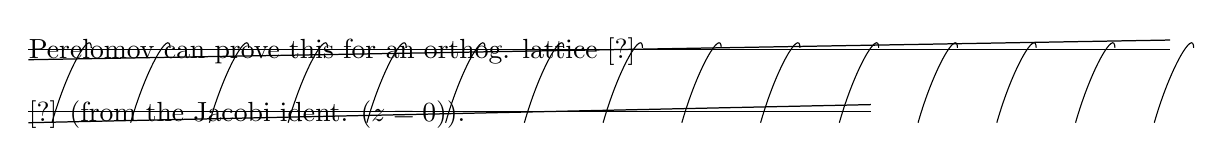
\begin{tikzpicture}[x=1mm, y=1mm]
\node[anchor=west, inner sep=0]at (0,0){Perelomov can prove this for an orthog. lattice [?]};
\node[anchor=west, inner sep=0]at (0,-8){[?] (from the Jacobi ident. $(z=0)$).};
\draw[line width=.45pt](0,.3)--(145,.3);
\draw[line width=.45pt](0,-1)--(145,1.5);
\draw[line width=.45pt](0,-7.6)--(107,-7.6);
\draw[line width=.45pt](0,-9)--(107,-6.7);
\foreach \x in {3,13,23,33,43,53,63,73,83,93,103,113,123,133,143}{\draw[line width=.4pt](\x,-9)..controls(\x+2,-2)and(\x+5,3)..(\x+5,.5);}
\end{tikzpicture}}\end{minipage}}}\par\smallskip }
\end{GelfandAdjacentEvidence}
\begin{GelfandAdjacentEvidence}{GELFAND-P000358}{2}

\noindent\makebox[0pt][r]{$\pi$\quad}The gen. ident. is \uline{not deduced} from the Jacobi \uline{ident.}.
\Unclear{GELFAND-P000358}{from-rewrite}{The current preposition is provisionally read “from”; it is rewritten in dark strokes. The earlier entry underneath is not securely separated.}
\end{GelfandAdjacentEvidence}
\begin{GelfandAdjacentEvidence}{GELFAND-P000358}{3}

This carries over to the $N$-dim. case.
Obtain $2^{N-1}(2^N-1)$ identities.
Thus, an elem. problem:
\begin{equation*}\sum (-1)^{mn+n+m}e^{-\frac12|\lambda_{mn}|^2+\lambda_{mn}z}=0,\end{equation*}
\Unclear{GELFAND-P000358}{identity-final-z}{The exponent ends in a crossed $z$. The upper stroke belongs to the letter; a separate bar above it is not discernible. The preliminary reading $\bar z$ is not adopted.}
\end{GelfandAdjacentEvidence}

if the lattice area $=\pi$.
\uline{Proof}: consider a Hilb. space with
\begin{equation*}\int\bar f (z)g (z)e^{-|z|^2}\, dz\, d\bar z.\end{equation*}
\noindent $|\boldsymbol{\lambda}_{mn}\rangle$

\begin{GelfandAdjacentEvidence}{GELFAND-P000358}{4}
Consider $|\lambda\rangle$ and $|\psi\rangle\in\mathcal H$.
\begin{center}\GelfandFitDiagram{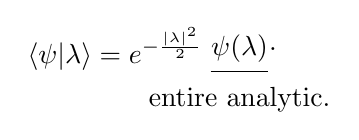
\begin{tikzpicture}
\node[inner sep=0](lhs)at (0,0){$\displaystyle\langle\psi|\lambda\rangle=e^{-\frac{|\lambda|^2}{2}}$};
\node[anchor=west, inner sep=0](psi)at ([xshift=1mm]lhs.east){$\displaystyle\psi (\lambda)$};
\node[anchor=west, inner sep=0]at (psi.east){.};
\draw[line width=.5pt]([yshift=-1mm]psi.south west)--([yshift=-1mm]psi.south east);
\node[anchor=north, inner sep=0]at ([yshift=-3mm]psi.south){entire analytic.};
\end{tikzpicture}}\end{center}
\uline{Orthog.}
\begin{equation*}\langle\psi|\lambda_{mn}\rangle=e^{-\frac{|\lambda|^2}{2}}\psi (\lambda_{mn}).\end{equation*}
\Unclear{GELFAND-P000358}{norm-denominator}{The second formula has $\lambda$ without $mn$ in the norm; the ket and the argument of $\psi$ have $\lambda_{mn}$. No subscripts are added to the norm.}
\end{GelfandAdjacentEvidence}
\begin{GelfandAdjacentEvidence}{GELFAND-P000358}{5}

\uline{Entire with 0s at the prescribed set of points.}
Need to prove that it does not exist in $F_2$.
(see Levin, \uline{standard} \uline{theorem}).
\Incomplete{GELFAND-P000358}{cancelled-matrix-prefix}{The isolated crossed-out mark before $G$ is not recovered in full.}
\end{GelfandAdjacentEvidence}
\begin{GelfandAdjacentEvidence}{GELFAND-P000358}{6}

\begin{equation*}G=\begin{pmatrix}1&\alpha&\delta\\0&1&\beta\\0&0&1\end{pmatrix},\end{equation*}
$\alpha,\beta,\delta$ --- real.



\SourceFigure{GELFAND-P000358}{lattice-caption-geometry}{The current $\alpha$ and $\beta$ in $\Gamma$ are heavily overwritten; earlier strokes are unrecovered. The upper right entry is provisionally shown as $k\pi$. The note below has a capital $K$. Below $L$ is a short detached vertical stroke towards the two underlined words “Our lattice”; its exact connection is not established.\par\smallskip\centering{\color{black}\GelfandFitDiagram{\begin{minipage}{148mm}\raggedright \GelfandFitDiagram{\begin{tikzpicture}
\node[inner sep=0](matrix)at (0,0){$\displaystyle\Gamma=\begin{pmatrix}1&\boldsymbol{\alpha}&k\pi\\0&1&\boldsymbol{\beta}\\0&0&1\end{pmatrix}.$};
\node[anchor=west, inner sep=0](membership)at ([xshift=12mm]matrix.east){$\alpha+i\beta\in$};
\node[anchor=west, inner sep=0](lattice)at ([xshift=1mm]membership.east){$L$};
\draw[line width=.5pt]([yshift=-2mm]lattice.south)--([yshift=-5mm]lattice.south);
\node[anchor=north west, inner sep=0, align=left]at ([xshift=-3mm, yshift=-8mm]lattice.south){\uline{Our}\\\uline{lattice.}};
\node[anchor=north, inner sep=0]at ([xshift=8mm, yshift=-5mm]matrix.south){$K$ --- integer.};
\end{tikzpicture}}\end{minipage}}}\par\smallskip }
\end{GelfandAdjacentEvidence}



\Needspace{7\baselineskip}
\SourcePage{GELFAND-P000359}{unlabelled}
Consider the operators.
\begin{equation*}\uline{D=e^{i\varphi}e^{i (\alpha^*a-\alpha a^*)}}\text{ --- a 3-param. group.}\end{equation*}
Lie alg. --- $a, a^+$ and $1$; $[a, a^+]=1$, other commutators $0$.
$\Gamma$ --- the $\alpha$-points of the lattice; $\varphi$ --- $0$ and $\pi$.
Then the repr. induced by the repr. $(-1)^{mn+m+n}$ of the discrete group $\Gamma$ is irreducible.
There is an extension to an \uline{arbitrary group}.

\begin{GelfandAdjacentEvidence}{GELFAND-P000359}{1}
\noindent\uline{Kazhdan.}
\Unclear{GELFAND-P000359}{margin-name}{“Kazhdan.” is shown provisionally; compressed middle strokes also permit the literal “Kamdan.”.}
\end{GelfandAdjacentEvidence}
\begin{GelfandAdjacentEvidence}{GELFAND-P000359}{2}

$G$ --- a polupr. group,
\Unclear{GELFAND-P000359}{group-word}{After $G$ --- “polupr.” is shown provisionally; “polugr.” remains a candidate. The abbreviation is not expanded.}
\end{GelfandAdjacentEvidence}
\begin{GelfandAdjacentEvidence}{GELFAND-P000359}{3}




\SourceFigure{GELFAND-P000359}{hilbert-insertion}{\par\smallskip\centering{\color{black}\GelfandFitDiagram{\begin{minipage}{148mm}\raggedright \GelfandFitDiagram{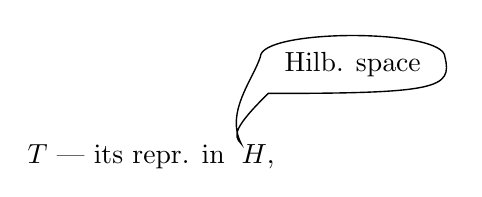
\begin{tikzpicture}
\node[inner sep=0](words)at (0,0){$T$ --- its repr. in};
\node[anchor=west, inner sep=0](space)at ([xshift=2mm]words.east){$H$,};
\node[inner sep=0](caption)at ([xshift=12mm, yshift=10mm]space.north){Hilb. space};
\draw[line width=.5pt]([xshift=-3mm,yshift=1mm]caption.west)..controls([xshift=-3mm,yshift=3mm]caption.north west)and([xshift=3mm,yshift=3mm]caption.north east)..([xshift=3mm,yshift=1mm]caption.east)..controls([xshift=4mm,yshift=-3mm]caption.east)and([xshift=2mm,yshift=-2mm]caption.south east)..([xshift=-2mm,yshift=-2mm]caption.south west)..controls([xshift=-1mm,yshift=2mm]space.north west)and([xshift=-1mm,yshift=1mm]space.north west)..(space.north west)..controls([xshift=-2mm,yshift=4mm]space.north west)and([xshift=-4mm,yshift=-2mm]caption.west)..([xshift=-3mm,yshift=1mm]caption.west);
\end{tikzpicture}}\end{minipage}}}\par\smallskip }
\end{GelfandAdjacentEvidence}
\begin{GelfandAdjacentEvidence}{GELFAND-P000359}{4}

$h_0$ --- a distinguished vector in $H$.
$T (g)h_0\in H$.
$\Gamma\subset G$ a discrete subgroup, $T (\gamma)h_0\in H$.
For a reasonable subgroup $\Gamma$ the system is complete and satisfies a finite number of relations.
Here --- a unipotent group.
\begin{center}\GelfandFitDiagram{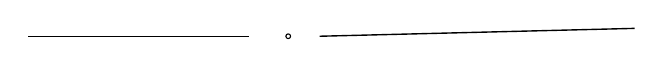
\begin{tikzpicture}[x=1mm, y=1mm]
\draw[line width=.5pt](0,0)--(28,0);
\draw[line width=.5pt](37,0)--(77,1);
\draw[line width=.4pt](33,0)circle(.3);
\end{tikzpicture}}\end{center}
\begin{equation*}f (z)=\sum_\alpha (-1)^{F (\alpha)}e^{-\frac\pi2H (\alpha,\alpha)+\pi H (\alpha, z)}=0=c\Theta (z).\end{equation*}
\Unclear{GELFAND-P000359}{theta-final-argument}{The exponent has $H (\alpha, z)$. No separate upper bar is discernible above the crossed $z$; the preliminary $H (\alpha,\bar z)$ is not adopted.}
\end{GelfandAdjacentEvidence}
\begin{GelfandAdjacentEvidence}{GELFAND-P000359}{5}

\Unclear{GELFAND-P000359}{zero-theta}{The source literally writes $=0=c\Theta (z)$. The last argument of $\Theta$ is repeatedly retraced, with overlapping upper and lower strokes. $z$ is shown provisionally; the earlier sign and any separate upper bar are not established.}
\end{GelfandAdjacentEvidence}
\begin{GelfandAdjacentEvidence}{GELFAND-P000359}{6}




\SourceFigure{GELFAND-P000359}{F-count-insertion}{\par\smallskip\centering{\color{black}\GelfandFitDiagram{\begin{minipage}{148mm}\raggedright \GelfandFitDiagram{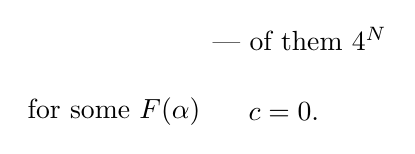
\begin{tikzpicture}
\node[inner sep=0](choices)at (0,0){for some $F (\alpha)$};
\node[anchor=west, inner sep=0](zero)at ([xshift=6mm]choices.east){$c=0$.};
\node[inner sep=0]at ([xshift=2mm, yshift=8mm]zero.north){--- of them \uline{$4^N$}};
\end{tikzpicture}}\end{minipage}}}\par\smallskip }
\end{GelfandAdjacentEvidence}

$c\ne0$ --- A new repr. of the $\Theta$-fn.
For half of the $F (\alpha)$ this is $0$.
$\Theta (z)$ --- the standard fn., $\ne0$.
\uline{Next meeting 1st Mon. of September.}


\Needspace{7\baselineskip}
\begin{GelfandAdjacentEvidence}{GELFAND-P000360}{1}
\SourcePage{GELFAND-P000360}{22}
\uuline{Kirillov} \uwave{on quantization}. (Kostant etc.)
\uline{Trivial} \uline{part.}
A symplectic manifold --- $X^{2n}$ --- even-dimensional with a nondeg. closed 2-form $\omega$ ($d\omega=0$).



\SourceFigure{GELFAND-P000360}{pq-insertion}{\par\smallskip\centering{\color{black}\GelfandFitDiagram{\begin{minipage}{68mm}\raggedright \GelfandFitDiagram{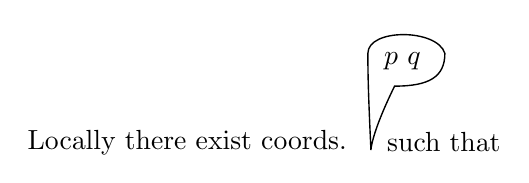
\begin{tikzpicture}
\node[inner sep=0](words)at (0,0){Locally there exist coords.};
\node[anchor=west, inner sep=0](that)at ([xshift=5mm]words.east){such that};
\node[inner sep=0](pq)at ([xshift=2mm, yshift=9mm]that.north west){$p\ q$};
\draw[line width=.5pt]([xshift=-2mm,yshift=1mm]pq.west)..controls([xshift=-2mm,yshift=3mm]pq.north west)and([xshift=2mm,yshift=3mm]pq.north east)..([xshift=3mm,yshift=1mm]pq.east)..controls([xshift=3mm,yshift=-2mm]pq.east)and([xshift=1mm,yshift=-2mm]pq.south east)..([xshift=-1mm,yshift=-2mm]pq.south)..controls([xshift=-2mm,yshift=1mm]that.west)and([xshift=-2mm,yshift=-1mm]that.west)..([xshift=-2mm,yshift=-1mm]that.west)..controls([xshift=-2mm,yshift=-2mm]pq.south west)and([xshift=-2mm,yshift=-1mm]pq.west)..([xshift=-2mm,yshift=1mm]pq.west);
\end{tikzpicture}}\end{minipage}}}\par\smallskip }
\end{GelfandAdjacentEvidence}

\begin{equation*}\omega=\sum_{i=1}^n dp_i\wedge dq_i.\end{equation*}
(see Rashevskii, “Geom. theory of diff. eqns.”, Sternberg, “Lectures on diff. geom.”).
Volume
\begin{equation*}\Omega=\frac1{n!}\omega\wedge\omega\wedge\cdots\wedge\omega=\frac1{n!}\omega^n\quad (\text{exterior power}).\end{equation*}
\begin{center}\GelfandFitDiagram{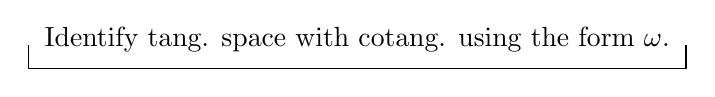
\begin{tikzpicture}
\node[inner sep=0](statement)at (0,0){Identify tang. space with cotang. using the form $\omega$.};
\draw[line width=.5pt]([xshift=-2mm,yshift=1mm]statement.south west)--([xshift=-2mm,yshift=-2mm]statement.south west)--([xshift=2mm,yshift=-2mm]statement.south east)--([xshift=2mm,yshift=1mm]statement.south east);
\end{tikzpicture}}\end{center}



\begin{GelfandAdjacentEvidence}{GELFAND-P000360}{2}
\begin{equation*}\omega (\xi,\eta)\text{:---}\quad\omega: T_xX\to T_x^*X\quad (\text{isomorphism}).\end{equation*}
\Unclear{GELFAND-P000360}{tangent-index}{The lower index of the first $T$ is heavily overwritten. $x$ with overlapping upper strokes is shown provisionally; $*$ remains a candidate.}
\end{GelfandAdjacentEvidence}

\begin{equation*}\xi\to\alpha_\xi;\end{equation*}
\begin{center}\GelfandFitDiagram{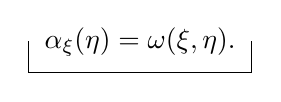
\begin{tikzpicture}
\node[inner sep=0](definition)at (0,0){$\displaystyle\alpha_\xi (\eta)=\omega (\xi,\eta). $};
\draw[line width=.5pt]([xshift=-2mm,yshift=2mm]definition.south west)--([xshift=-2mm,yshift=-2mm]definition.south west)--([xshift=2mm,yshift=-2mm]definition.south east)--([xshift=2mm,yshift=2mm]definition.south east);
\end{tikzpicture}}\end{center}



\begin{equation*}\left (\text{in those coords. }\frac{\partial}{\partial q_i}\to dp_i,\quad\frac{\partial}{\partial p_i}\to-dq_i\right).\end{equation*}
Closed 1-forms $\leftrightarrow$ vector fields preserving the form $\omega$.
\begin{flushright}in the sense of the Lie derivative $L_\xi$.\end{flushright}
$L_\xi$ acts on all geom. objects on the manifold.
$\varphi_t$ --- the corresponding one-param. group, corresponding to the field $\xi$. ($\dot x=\xi (x)$).
\begin{equation*}\left.\frac d{dt}\right|_{t=0}=L_\xi.\end{equation*}
It commutes with differentiation of diff. forms: $L_\xi d=dL_\xi$.
$L_\xi f=\xi f$, $L_\xi\eta=[\xi,\eta]$.
\begin{center}\fbox{$L_\xi\omega=0\ \Leftrightarrow\ d\alpha_\xi=0$}\end{center}



--- a short formulation.
Such fields --- \uline{Hamiltonian}, forms --- \uline{gradient}.
$\xi$ --- loc. Hamiltonian $\Leftrightarrow\alpha_\xi=df$.
$f$ is defined up to const and is multivalued.


\Needspace{7\baselineskip}
\begin{GelfandAdjacentEvidence}{GELFAND-P000361}{1}
\SourcePage{GELFAND-P000361}{unlabelled}



\Unclear{GELFAND-P000361}{hamiltonian-first-mark}{Beside the first $\xi_F$ is a dense round overwritten mark. It is shown as a round mark without assigning a mathematical meaning; the exact earlier sign is not established.\par\smallskip\centering{\color{black}\GelfandFitDiagram{\begin{minipage}{68mm}\raggedright \GelfandFitDiagram{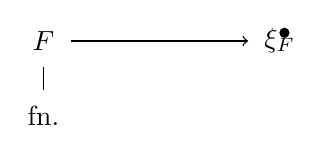
\begin{tikzpicture}
\node[inner sep=0](function)at (0,0){$F$};
\node[inner sep=0](field)at (30mm,0){$\xi_F$};
\draw[->,line width=.5pt]([xshift=2mm]function.east)--([xshift=-2mm]field.west);
\draw[line width=.5pt]([yshift=-2mm]function.south)--([yshift=-5mm]function.south);
\node[anchor=north, inner sep=0]at ([yshift=-7mm]function.south){fn.};
\fill([xshift=-1.4mm,yshift=-.6mm]field.north east)circle(.65mm);
\end{tikzpicture}}\end{minipage}}}\par\smallskip }
\end{GelfandAdjacentEvidence}
\begin{GelfandAdjacentEvidence}{GELFAND-P000361}{2}

$dF$ --- a form $\longleftrightarrow$ Hamiltonian field; $dF=2\alpha_{\xi_F}$.
Poisson bracket.
\begin{equation*}\{F_1, F_2\}=\xi_{F_1}F_2=-\xi_{F_2}F_1=2\omega (\xi_{F_1},\xi_{F_2}).\end{equation*}
\uline{Identity}:
\begin{equation*}\xi_{\{F_1, F_2\}}=[\xi_{F_1},\xi_{F_2}].\end{equation*}
\uline{Remark}:



\Unclear{GELFAND-P000361}{wedge-mark}{Between $(dp\wedge dq)$ and the parenthesis with vectors is a dense crossed hash-like mark. Its strokes are shown without a mathematical interpretation.\par\smallskip\centering{\color{black}\GelfandFitDiagram{\begin{minipage}{148mm}\raggedright \GelfandFitDiagram{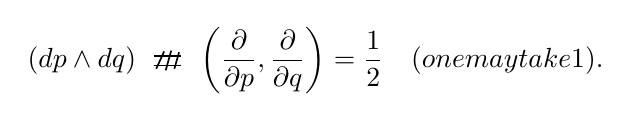
\begin{tikzpicture}
\node[inner sep=0](form)at (0,0){$\displaystyle (dp\wedge dq)$};
\coordinate (mark)at ([xshift=4mm]form.east);
\draw[line width=.6pt]([xshift=-1.5mm,yshift=-1mm]mark)--([xshift=-.5mm,yshift=1.2mm]mark);
\draw[line width=.6pt]([xshift=-.3mm,yshift=-1.2mm]mark)--([xshift=.4mm,yshift=1.3mm]mark);
\draw[line width=.6pt]([xshift=.8mm,yshift=-1mm]mark)--([xshift=1.4mm,yshift=1.1mm]mark);
\draw[line width=.6pt]([xshift=-1.8mm,yshift=.6mm]mark)--([xshift=1.7mm,yshift=.6mm]mark);
\draw[line width=.6pt]([xshift=-1.8mm,yshift=-.6mm]mark)--([xshift=1.7mm,yshift=-.6mm]mark);
\node[anchor=west, inner sep=0]at ([xshift=4mm]mark){$\displaystyle\left (\frac\partial{\partial p},\frac\partial{\partial q}\right)=\frac12\quad (\text{one may take }1). $};
\end{tikzpicture}}\end{minipage}}}\par\smallskip }
\end{GelfandAdjacentEvidence}
\begin{GelfandAdjacentEvidence}{GELFAND-P000361}{3}

\begin{equation*}\frac12[\alpha_1(\xi)\alpha_2(\eta)-\alpha_2(\xi)\alpha_1(\eta)]=\alpha_1\wedge\alpha_2.\end{equation*}
A \uline{new object} is constr. when $[\omega]\in H^2(X, Z)$.
Constr. a complex 1-dim. bundle and a map $C$.



\SourceFigure{GELFAND-P000361}{bundle-diagram}{\par\smallskip\centering{\color{black}\GelfandFitDiagram{\begin{minipage}{68mm}\raggedright \begin{equation*}\GelfandFitDiagram{\begin{tikzcd}[ampersand replacement=\&, ampersand replacement=\&]C\arrow[r]\&L\arrow[d]\\\&X\end{tikzcd}}\end{equation*}\end{minipage}}}\par\smallskip }
\end{GelfandAdjacentEvidence}
\begin{GelfandAdjacentEvidence}{GELFAND-P000361}{4}

$\{U_j\}$ --- a covering, $\omega=d\alpha_j$ in $U_j$.
On $U_j\cap U_k$ constr. $\alpha_j-\alpha_k=df_{jk}$.
\sout{$\alpha$}[?]
\Incomplete{GELFAND-P000361}{cancelled-cocycle}{After $df_{jk}$, the beginning of the crossed entry is provisionally shown as $\alpha$. Small signs, subscripts and the continuation are not recovered in full.}
\end{GelfandAdjacentEvidence}
\begin{GelfandAdjacentEvidence}{GELFAND-P000361}{5}

on $U_j\cap U_k\wedge U_\ell$ we have $d (f_{jk}+f_{k\ell}+f_{\ell j})=0$ and hence
\Unclear{GELFAND-P000361}{triple-overlap-wedge}{The second sign between the sets is pointed: $\wedge$ is shown provisionally, without replacing it by the usual intersection.}
\end{GelfandAdjacentEvidence}
\begin{GelfandAdjacentEvidence}{GELFAND-P000361}{6}




\SourceFigure{GELFAND-P000361}{constant-caption}{\par\smallskip\centering{\color{black}\GelfandFitDiagram{\begin{minipage}{148mm}\raggedright \GelfandFitDiagram{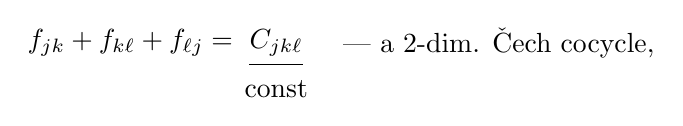
\begin{tikzpicture}
\node[inner sep=0](sum)at (0,0){$\displaystyle f_{jk}+f_{k\ell}+f_{\ell j}=$};
\node[anchor=west, inner sep=0](constant)at ([xshift=2mm]sum.east){$\displaystyle C_{jk\ell}$};
\draw[line width=.5pt]([yshift=-1mm]constant.south west)--([yshift=-1mm]constant.south east);
\node[anchor=north, inner sep=0]at ([yshift=-3mm]constant.south){const};
\node[anchor=west, inner sep=0]at ([xshift=5mm]constant.east){--- a 2-dim. Čech cocycle,};
\end{tikzpicture}}\end{minipage}}}\par\smallskip }
\end{GelfandAdjacentEvidence}

corresponding to the form \uuline{$\omega$}.
Integer-valued --- $\exists\alpha_j, f_{jk}$ such that $C_{jk\ell}$ --- integer-valued.
\begin{equation*}g_{jk}=e^{2\pi if_{jk}}\text{ --- a set of bundle transition fns.}\quad (\text{1-dim.}).\end{equation*}
\begin{center}\GelfandFitDiagram{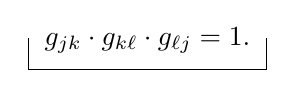
\begin{tikzpicture}
\node[inner sep=0](transition)at (0,0){$\displaystyle g_{jk}\cdot g_{k\ell}\cdot g_{\ell j}=1.$};
\draw[line width=.5pt]([xshift=-2mm,yshift=2mm]transition.south west)--([xshift=-2mm,yshift=-2mm]transition.south west)--([xshift=2mm,yshift=-2mm]transition.south east)--([xshift=2mm,yshift=2mm]transition.south east);
\end{tikzpicture}}\end{center}





\Needspace{7\baselineskip}
\begin{GelfandAdjacentEvidence}{GELFAND-P000362}{1}
\SourcePage{GELFAND-P000362}{23}
Choose other $\alpha$,
\sout{[?] const [?]}
\Incomplete{GELFAND-P000362}{cancelled-opening}{In the cancelled continuation a const-like fragment is shown provisionally. Other words and signs among long looping cancellation strokes are not read in full.}
\end{GelfandAdjacentEvidence}

The equiv. class of the constr. bundle depends on choosing an element of
\begin{center}\GelfandFitDiagram{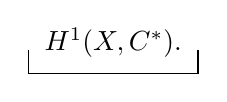
\begin{tikzpicture}
\node[inner sep=0](class)at (0,0){$H^1(X,\mathbb C^*)$.};
\draw[line width=.5pt]([xshift=-2mm,yshift=1mm]class.south west)--([xshift=-2mm,yshift=-2mm]class.south west)--([xshift=2mm,yshift=-2mm]class.south east)--([xshift=2mm,yshift=1mm]class.south east);
\end{tikzpicture}}\end{center}



\begin{GelfandAdjacentEvidence}{GELFAND-P000362}{2}
$H^1(X,\mathbb C^*)$ acts simply transitively on the set of bundles.
($\mathbb C^*$, rather than
\Incomplete{GELFAND-P000362}{cancelled-sheaf}{The small crossed-out token before “sheaf” is wholly unreadable.}
\end{GelfandAdjacentEvidence}

the sheaf of continuous fns.)
$s_j$ in $U_j$, $s_j=g_{jk}s_k$ --- a section of the bundle.



\begin{GelfandAdjacentEvidence}{GELFAND-P000362}{3}
along a vector field.
\SourceFigure{GELFAND-P000362}{derivative-outline}{\par\smallskip\centering{\color{black}\GelfandFitDiagram{\begin{minipage}{148mm}\raggedright \GelfandFitDiagram{
\begin{tikzpicture}
\node[inner sep=0](prefix)at (0,0){\uline{Connection} ---};
\node[anchor=west, inner sep=0](derivative)at ([xshift=4mm]prefix.east){derivative};
\node[anchor=west, inner sep=0]at ([xshift=4mm]derivative.east){of sections};
\draw[line width=.5pt]([xshift=-2mm]derivative.west)..controls([xshift=-1mm,yshift=4mm]derivative.north west)and([xshift=1mm,yshift=3mm]derivative.north east)..([xshift=2mm,yshift=2mm]derivative.east)..controls([xshift=3mm,yshift=-3mm]derivative.east)and([xshift=1mm,yshift=-3mm]derivative.south east)..([xshift=-1mm,yshift=-2mm]derivative.south west)--([xshift=-2mm]derivative.west);
\draw[line width=.5pt]([xshift=1mm,yshift=3mm]derivative.north east)--([xshift=3mm,yshift=2mm]derivative.north east);
\draw[line width=.5pt]([xshift=1mm,yshift=2mm]derivative.north east)--([xshift=3mm,yshift=3mm]derivative.north east);
\end{tikzpicture}}\end{minipage}}}\par\smallskip }
\end{GelfandAdjacentEvidence}
\begin{GelfandAdjacentEvidence}{GELFAND-P000362}{4}




\Unclear{GELFAND-P000362}{nabla-domain}{The small upper mark on the first $\Gamma$ is thickened. $\Gamma^1(L)$ is shown provisionally; $\Gamma\prime (L)$ remains a candidate. Below $\nabla_\xi$ is a curved underline.\par\smallskip\centering{\color{black}\GelfandFitDiagram{\begin{minipage}{68mm}\raggedright \GelfandFitDiagram{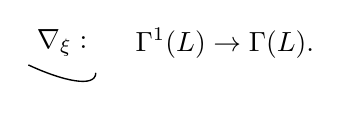
\begin{tikzpicture}
\node[inner sep=0](nabla)at (0,0){$\displaystyle\nabla_\xi: $};
\node[anchor=west, inner sep=0]at ([xshift=6mm]nabla.east){$\displaystyle\Gamma^1(L)\to\Gamma (L). $};
\draw[line width=.5pt]([xshift=-1mm,yshift=-1mm]nabla.south west)..controls([yshift=-3mm]nabla.south)and([xshift=1mm,yshift=-4mm]nabla.south east)..([xshift=1mm,yshift=-2mm]nabla.south east);
\end{tikzpicture}}\end{minipage}}}\par\smallskip }
\end{GelfandAdjacentEvidence}
\begin{GelfandAdjacentEvidence}{GELFAND-P000362}{5}




\SourceFigure{GELFAND-P000362}{choice-marginal}{\par\smallskip\centering{\color{black}\GelfandFitDiagram{\begin{minipage}{68mm}\raggedright \begin{flushright}\GelfandFitDiagram{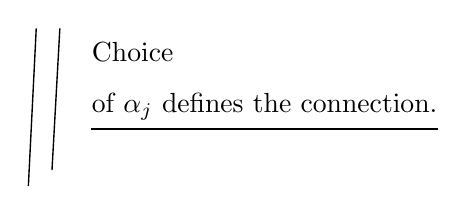
\begin{tikzpicture}[x=1mm, y=1mm]
\node[anchor=west, inner sep=0]at (0,0){\uline{Choice}};
\node[anchor=west, inner sep=0](choice)at (0,-7){of $\alpha_j$ defines the connection.};
\draw[line width=.5pt]([yshift=-1mm]choice.south west)--([yshift=-1mm]choice.south east);
\draw[line width=.5pt](-4,3)--(-5,-15);
\draw[line width=.5pt](-7,3)--(-8,-17);
\end{tikzpicture}}\end{flushright}\end{minipage}}}\par\smallskip }
\end{GelfandAdjacentEvidence}

\begin{center}\GelfandFitDiagram{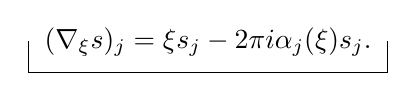
\begin{tikzpicture}
\node[inner sep=0](connection)at (0,0){$\displaystyle (\nabla_\xi s)_j=\xi s_j-2\pi i\alpha_j (\xi)s_j. $};
\draw[line width=.5pt]([xshift=-2mm,yshift=2mm]connection.south west)--([xshift=-2mm,yshift=-2mm]connection.south west)--([xshift=2mm,yshift=-2mm]connection.south east)--([xshift=2mm,yshift=2mm]connection.south east);
\end{tikzpicture}}\end{center}



\begin{GelfandAdjacentEvidence}{GELFAND-P000362}{6}
This acts as an oper. on the space of sections. (checking left to the reader).
\Unclear{GELFAND-P000362}{reader-proof-note}{The first word is provisionally read “checking”; “to check” remains a candidate. The following Russian abbreviations are “predost. chit.”, with a separate o-like loop after d. The abbreviations remain unexpanded in the Russian text.}
\end{GelfandAdjacentEvidence}
\begin{GelfandAdjacentEvidence}{GELFAND-P000362}{7}

\uline{Check}:
\begin{equation*}(\nabla_\xi s)_j=g_{jk}(\nabla_\xi s)_k.\end{equation*}
Define a Hermitian bundle with a connection and a generalized Fourier transform in it.
Consider an arbitrary 1st-order diff. oper. in the bundle $L$.
\begin{equation*}D:\Gamma (L)\to\Gamma (L)\quad (\text{ordinary in local coords.}).\end{equation*}
Its gen. form: $D=\nabla_\xi+\varphi=D_{\xi,\varphi}$ ($\varphi$ --- multiplication by a fn.).



\Incomplete{GELFAND-P000362}{compatible-cancelled}{The earlier adjective is crossed out and not recovered in full. Above it is the legible inserted and outlined word “compatible”.\par\smallskip\centering{\color{black}\GelfandFitDiagram{\begin{minipage}{148mm}\raggedright \GelfandFitDiagram{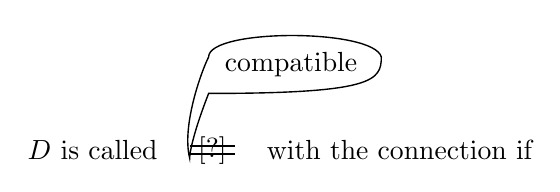
\begin{tikzpicture}
\node[inner sep=0](prefix)at (0,0){$D$ is called};
\node[anchor=west, inner sep=0](old)at ([xshift=5mm]prefix.east){[?]};
\draw[line width=.5pt]([xshift=-1mm,yshift=.5mm]old.west)--([xshift=1mm,yshift=.5mm]old.east);
\draw[line width=.5pt]([xshift=-1mm,yshift=-.5mm]old.west)--([xshift=1mm,yshift=-.5mm]old.east);
\node[inner sep=0](new)at ([xshift=10mm, yshift=9mm]old.north){compatible};
\draw[line width=.5pt]([xshift=-2mm,yshift=1mm]new.west)..controls([xshift=-2mm,yshift=3mm]new.north west)and([xshift=2mm,yshift=3mm]new.north east)..([xshift=3mm,yshift=1mm]new.east)..controls([xshift=3mm,yshift=-2mm]new.east)and([xshift=2mm,yshift=-2mm]new.south east)..([xshift=-2mm,yshift=-2mm]new.south west)..controls([xshift=-1mm,yshift=1mm]old.west)and([xshift=-1mm,yshift=-1mm]old.west)..([xshift=-1mm,yshift=-1mm]old.west)..controls([xshift=-2mm,yshift=3mm]old.west)and([xshift=-3mm,yshift=-1mm]new.west)..([xshift=-2mm,yshift=1mm]new.west);
\node[anchor=west, inner sep=0]at ([xshift=5mm]old.east){with the connection if};
\end{tikzpicture}}\end{minipage}}}\par\smallskip }
\end{GelfandAdjacentEvidence}
\begin{GelfandAdjacentEvidence}{GELFAND-P000362}{8}




\SourceFigure{GELFAND-P000362}{right-commutator-arrow}{An arc starts at the right of the commutator, bows to the right beside the remarks in square brackets, and ends down-left above the lower frame. No additional mathematical relation is assigned to the arc.\par\smallskip\centering{\color{black}\GelfandFitDiagram{\begin{minipage}{148mm}\raggedright \GelfandFitDiagram{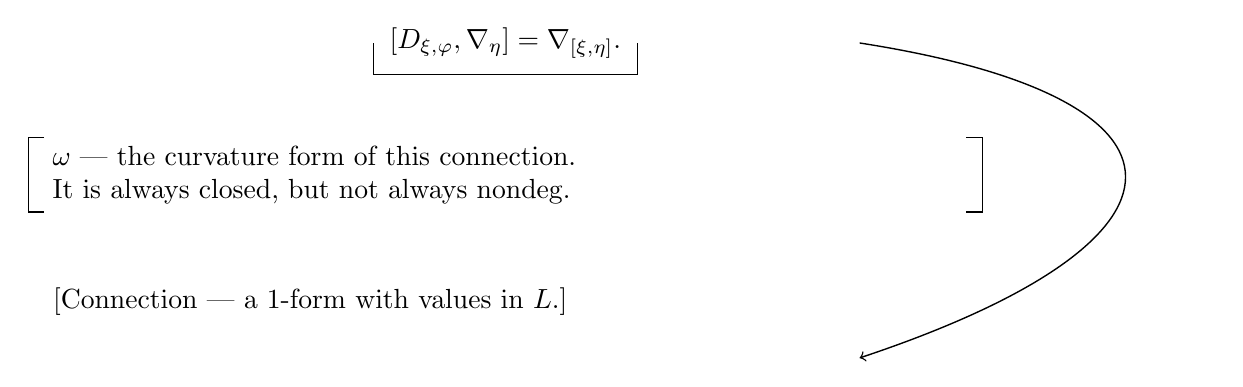
\begin{tikzpicture}[x=1mm, y=1mm]
\node[inner sep=0](commutator)at (0,0){$\displaystyle[D_{\xi,\varphi},\nabla_\eta]=\nabla_{[\xi,\eta]}.$};
\draw[line width=.5pt]([xshift=-2mm,yshift=2mm]commutator.south west)--([xshift=-2mm,yshift=-2mm]commutator.south west)--([xshift=2mm,yshift=-2mm]commutator.south east)--([xshift=2mm,yshift=2mm]commutator.south east);
\node[anchor=north, inner sep=0, align=left, text width=115mm](curvature)at (0,-13){$\omega$ --- the curvature form of this connection.\\It is always closed, but not always nondeg.};
\draw[line width=.5pt]([xshift=-1mm,yshift=1mm]curvature.north west)--([xshift=-3mm,yshift=1mm]curvature.north west)--([xshift=-3mm,yshift=-1mm]curvature.south west)--([xshift=-1mm,yshift=-1mm]curvature.south west);
\draw[line width=.5pt]([xshift=1mm,yshift=1mm]curvature.north east)--([xshift=3mm,yshift=1mm]curvature.north east)--([xshift=3mm,yshift=-1mm]curvature.south east)--([xshift=1mm,yshift=-1mm]curvature.south east);
\node[anchor=north west, inner sep=0]at (-57.5,-31){[Connection --- a 1-form with values in $L$.]};
\draw[->,line width=.5pt](45,0)..controls(90,-7)and(90,-25)..(45,-40);
\end{tikzpicture}}\end{minipage}}}\par\smallskip }
\end{GelfandAdjacentEvidence}
\begin{GelfandAdjacentEvidence}{GELFAND-P000362}{9}

Or
\begin{center}\fbox{$\xi=\frac1{\pi i}\xi_\varphi$}\end{center}
\Unclear{GELFAND-P000362}{normalization}{The frame literally reads $\xi=\frac1{\pi i}\xi_\varphi$.}
\end{GelfandAdjacentEvidence}

(in particular, $\xi$ is actually Hamiltonian.)


\Needspace{7\baselineskip}
\begin{GelfandAdjacentEvidence}{GELFAND-P000363}{1}
\SourcePage{GELFAND-P000363}{unlabelled}
\sout{$D_\varphi$}
\Unclear{GELFAND-P000363}{cancelled-initial}{The crossed initial sign is provisionally shown as $D_\varphi$; overlapping strokes do not permit a secure reading.}
\end{GelfandAdjacentEvidence}
\begin{GelfandAdjacentEvidence}{GELFAND-P000363}{2}

The operator $D_\varphi=\nabla_{\xi_\varphi}+\pi i\varphi:\Gamma (L)\to\Gamma (L)$.
\uline{Fund. theorem}:
\begin{equation*}[D_\varphi, D_\psi]=D_{\{\varphi,\psi\}}.\end{equation*}
(obtain a repr. of the Lie algebra) compatible with the connection.
(Van Hove repr.: fns. $\to$ opers. on bundle sections) compatible with the connection.
\uwave{This is called prequantization}.



\SourceFigure{GELFAND-P000363}{prequant-margin-arrow}{Before the note at right is a short left arrow with a shaft on its right. Its exact endpoint is not established; no additional logical connection is assigned.\par\smallskip\centering{\color{black}\GelfandFitDiagram{\begin{minipage}{148mm}\raggedright \begin{flushright}$\leftarrow$ acts on too large a space.\end{flushright}\end{minipage}}}\par\smallskip }
\end{GelfandAdjacentEvidence}

(\sout{This.} consider 200 pp. of the 3rd issue of Lectures on Modern An., Lecture Notes,
\uwave{Lectures on Modern Analysis}, $\overline{\underline{\mathrm{III}}}$).
A \uline{Lagrangian} \uline{distribution} (isotropic space) ---
--- at $\forall$ point a Lagr. subspace is given. $\frac12$ the dimension.
\begin{equation*}F: F_x\subset T_*X,\qquad\omega|_{F_x}=0,\qquad\dim F_x=n=\frac12\dim X.\end{equation*}
Complex distributions will be considered:
\begin{equation*}F_x\subset T_x^CX,\qquad\omega|_{F_x}=0,\qquad\dim_C F_x=n=\frac12\dim X.\end{equation*}
The choice of an integr. Lagr. distrib. --- \uuline{polarization}.



\begin{GelfandAdjacentEvidence}{GELFAND-P000363}{3}
It is considered integrable (Frobenius cond.) --- see \uline{Dieudonné}.
(Locally exists --- because of $\sum dp\wedge dq$) take the $p$-subspace.



\SourceFigure{GELFAND-P000363}{complex-marginal}{\par\smallskip\centering{\color{black}\GelfandFitDiagram{\begin{minipage}{68mm}\raggedright \begin{flushright}\GelfandFitDiagram{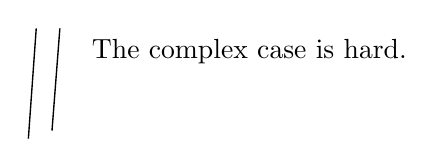
\begin{tikzpicture}[x=1mm, y=1mm]
\node[anchor=west, inner sep=0]at (0,0){The complex case is hard.};
\draw[line width=.5pt](-4,3)--(-5,-10);
\draw[line width=.5pt](-7,3)--(-8,-11);
\end{tikzpicture}}\end{flushright}\end{minipage}}}\par\smallskip }
\end{GelfandAdjacentEvidence}

\uline{Example}: a sphere with its usual volume. Globally impossible.
\uline{Special cases} (extreme).

\begin{GelfandAdjacentEvidence}{GELFAND-P000363}{4}
1) $\overline{\boldsymbol F}_x=F_x$ --- a real distribution. (\uline{real polarization})
\Unclear{GELFAND-P000363}{real-polarization-overwrite}{The first $F$ and its bar in the first equality are heavily thickened or rewritten. The current reading is provisionally shown as $\bar F_x=F_x$; earlier strokes are not separated.}
\end{GelfandAdjacentEvidence}

2) $F_x\cap\bar F_x=0.$ (Kahler \uline{polarization}).
\begin{equation*}\dim (F_x+\bar F_x)=k\quad (=\mathrm{const})\quad (\text{and an integr. bundle}).\end{equation*}
There is a mixed-mfd. structure there (a bundle with a real base and complex fibres; transitions --- holom. transformations of the fibres).


\Needspace{7\baselineskip}
\begin{GelfandAdjacentEvidence}{GELFAND-P000364}{1}
\SourcePage{GELFAND-P000364}{24}
$F$ --- a distrib., $\Gamma (L, F)$ --- sections constant along the leaves, i.e., $\nabla_\xi s=0$ if $\xi_x\in F_x$.
Now consider the action of opers. on \uuline{$\Gamma (L, F)$}.



\SourceFigure{GELFAND-P000364}{algebra-caption}{\par\smallskip\centering{\color{black}\GelfandFitDiagram{\begin{minipage}{148mm}\raggedright \GelfandFitDiagram{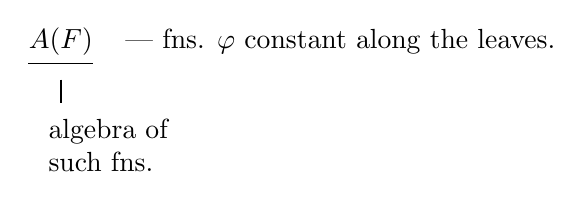
\begin{tikzpicture}
\node[inner sep=0](algebra)at (0,0){$A (F)$};
\draw[line width=.5pt]([yshift=-1mm]algebra.south west)--([yshift=-1mm]algebra.south east);
\node[anchor=west, inner sep=0]at ([xshift=4mm]algebra.east){--- fns. $\varphi$ constant along the leaves.};
\draw[line width=.5pt]([yshift=-3mm]algebra.south)--([yshift=-6mm]algebra.south);
\node[anchor=north, inner sep=0, align=left]at ([xshift=6mm, yshift=-8mm]algebra.south){algebra of\\such fns.};
\end{tikzpicture}}\end{minipage}}}\par\smallskip }
\end{GelfandAdjacentEvidence}
\begin{GelfandAdjacentEvidence}{GELFAND-P000364}{2}

($\xi f=0$, \sout{$\forall$}
\Unclear{GELFAND-P000364}{cancelled-forall}{The crossed sign is provisionally shown as $\forall$; overlapping diagonal strokes cross it.}
\end{GelfandAdjacentEvidence}
\begin{GelfandAdjacentEvidence}{GELFAND-P000364}{3}

if $\xi_x\in F_x$).
$\varphi\in A (F)\Rightarrow D_\varphi$ preserves the space of sections ($D_\varphi$ acts on $\Gamma (L, F)$ as multiplication by $\varphi$).
\uwave{$A (F)$ --- a max. commutative subalg. with the Poisson bracket} (locally).
Now consider operators (also preserving $\Gamma (L, F)$)
\begin{equation*}\begin{aligned}A_1(F)&=\text{normalizer of }A (F)\text{ in the Poisson-bracket alg.}=\\&=\{\varphi:\{\varphi, A (F)\}\subset A (F)\}.\end{aligned}\end{equation*}
\uuline{Thm.} Operators $D_\varphi$ with $\varphi\in A_1(F)$ preserve $\Gamma (L, F)$ and act there as 1st-order opers.
This is already \uline{quantization}, and the fns. --- quantizing.
(Other quant. are already nonunique).
There are many of them.
\Unclear{GELFAND-P000364}{overwritten-their}{The current word “ikh” (“of them”) is readable, but its first letter is rewritten. Earlier strokes are not separated.}
\end{GelfandAdjacentEvidence}

$p, q$; $dq=0$ --- subspace, fns. --- of $q$ only.
\uline{Opers.} --- fns. of $q$ --- multiplication opers., linear fns. of $p$ --- 1st-order opers.
\begin{center}\GelfandFitDiagram{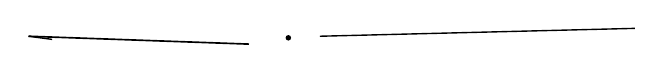
\begin{tikzpicture}[x=1mm, y=1mm]
\draw[line width=.6pt](0,0)--(28,-1);
\draw[line width=.5pt](0,0)--(3,-.4);
\draw[line width=.5pt](37,0)--(77,1);
\fill(33,-.2)circle(.35);
\end{tikzpicture}}\end{center}
\uline{Next time}: \uuline{Kirillov.}


\Needspace{7\baselineskip}
\begin{GelfandAdjacentEvidence}{GELFAND-P000365}{1}
\SourcePage{GELFAND-P000365}{unlabelled}
\uuline{13/$\overline{\underline{\mathrm{IX}}}$-71.}
\uuline{I. M. Gelfand} \uuline{on} \uuline{the work} \uuline{of Springer} (comput. char. for semisimple groups over a finite field).
1. \uwave{Consider} \uwave{the group} $SL (n, C)$ and unipot. matrices. [?]
\Unclear{GELFAND-P000365}{uni-prefix}{A separate dark overwritten sign precedes the first matrix. Neither $U$ nor an equals sign has been established securely.}
\end{GelfandAdjacentEvidence}
\begin{GelfandAdjacentEvidence}{GELFAND-P000365}{2}

\begin{equation*}\begin{pmatrix}1&&&0\\&1&&\\&&\ddots&\\\dots&&&1\end{pmatrix}\end{equation*}
\sout{$U$}[?]
\Incomplete{GELFAND-P000365}{uni-cancel}{The beginning of the short cancelled entry is provisionally shown as a $U$-like sign. The remaining signs under horizontal strokes have not been read in full.}
\end{GelfandAdjacentEvidence}
\begin{GelfandAdjacentEvidence}{GELFAND-P000365}{3}

(reduced to this form). $(1+a,\ \text{where }a^n=0)$.
At $1$ --- sing. points.
\begin{equation*}\begin{pmatrix}a&b\\c&d\end{pmatrix},\quad ad-bc=1,\qquad\text{unipot. }a+d=2,\quad\text{in }R^3\text{ a cone,}\quad1\text{ --- a singularity.}\end{equation*}
\uuline{Nonsingular} --- one Jordan block.
\uwave{Several Jordan blocks} --- \textbf{singular}.
\uline{Answer}: $R$ --- the set



\Incomplete{GELFAND-P000365}{answer-cancel}{Beneath the outlined insertion “all unipot. matrices”, the earlier phrase is cancelled. Its remainder between and after the provisionally legible fragments has not been recovered.\par\smallskip\centering{\color{black}\GelfandFitDiagram{\begin{minipage}{148mm}\raggedright \GelfandFitDiagram{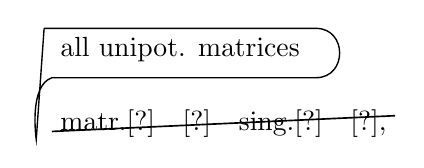
\begin{tikzpicture}
\node[inner sep=0](old)at (0,0){\sout{matr.[?]\quad[?]\quad sing.[?]\quad[?]},};
\node[anchor=south west, inner sep=0](new)at ([yshift=6mm]old.north west){all unipot. matrices};
\draw[line width=.5pt]([xshift=-2mm,yshift=1mm]new.north west)--([xshift=2mm,yshift=1mm]new.north east)..controls([xshift=6mm,yshift=1mm]new.north east)and([xshift=6mm,yshift=-2mm]new.south east)..([xshift=2mm,yshift=-2mm]new.south east)--([xshift=-1mm,yshift=-2mm]new.south west)..controls([xshift=-4mm,yshift=-3mm]new.south west)and([xshift=-3mm,yshift=-2mm]old.west)..([xshift=-3mm,yshift=-2mm]old.west)--([xshift=-2mm,yshift=1mm]new.north west);
\draw[line width=.6pt]([xshift=-1mm,yshift=-1mm]old.west)--([xshift=1mm,yshift=1mm]old.east);
\end{tikzpicture}}\end{minipage}}}\par\smallskip }
\end{GelfandAdjacentEvidence}
\begin{GelfandAdjacentEvidence}{GELFAND-P000365}{4}

\Unclear{GELFAND-P000365}{answer-cancel-fragments}{The contractions “matr.” and “sing.” are provisionally rendered in the cancelled line. Endings and intervening writing are covered by strokes; the contractions are not expanded.}
\end{GelfandAdjacentEvidence}
\begin{GelfandAdjacentEvidence}{GELFAND-P000365}{5}

$g\in R$.



\Unclear{GELFAND-P000365}{projective-cancel}{Between $P=$ and $B\backslash G$ a sign is heavily cancelled, provisionally $P$. The exact earlier sign has not been recovered. Beneath it is a short vertical stroke and the caption “project. space.”.\par\smallskip\centering{\color{black}\GelfandFitDiagram{\begin{minipage}{148mm}\raggedright \GelfandFitDiagram{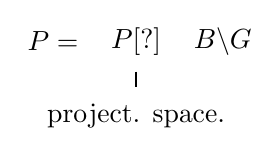
\begin{tikzpicture}
\node[inner sep=0](prefix)at (0,0){$P=$};
\node[anchor=west, inner sep=0](cancelled)at ([xshift=4mm]prefix.east){\sout{$P$}[?]};
\node[anchor=west, inner sep=0]at ([xshift=4mm]cancelled.east){$B\backslash G$};
\draw[line width=.5pt]([yshift=-2mm]cancelled.south)--([yshift=-4mm]cancelled.south);
\node[anchor=north, inner sep=0]at ([yshift=-6mm]cancelled.south){project. space.};
\end{tikzpicture}}\end{minipage}}}\par\smallskip }
\end{GelfandAdjacentEvidence}
\begin{GelfandAdjacentEvidence}{GELFAND-P000365}{6}

$B$ --- triangular matrices
\begin{equation*}\begin{pmatrix}\lambda_1&&0\\&\ddots&\\\dots&&\lambda_n\end{pmatrix}.\end{equation*}
Consider pairs $(p, g)$ with actions
\begin{equation*}pgp^{-1}\in U=\left\{\begin{pmatrix}1&&&0\\&1&&\\&&\ddots&\\\dots&&&1\end{pmatrix}\right\},\qquad p\in P.\end{equation*}
(This does not depend on the chosen representative elem. from $p$.)
$\bar R$ --- the set of pairs.
\begin{equation*}(p, g)\longrightarrow g.\end{equation*}
This is $\bar R\to R$, a resolution of singularities (all).
Over a point in gen. position \uline{one element.}
$\bar R$ --- a nonsingular variety.
(This is for an arbitrary \uwave{reductive} \uwave{group} over $\forall$ field.)
\Unclear{GELFAND-P000365}{reductive-overwritten}{The Russian word “nad” (“over”) is readable, but its last letter is heavily rewritten, with a separate arc above it. Earlier strokes are not separated.}
\end{GelfandAdjacentEvidence}
\begin{GelfandAdjacentEvidence}{GELFAND-P000365}{7}

2. \uline{Geom. interpretation of Hall polynomials.}
Consider $G$ [?]
\Incomplete{GELFAND-P000365}{group-overwrite}{After $G$ is a short overwritten and cancelled group of strokes. An equals sign remains a candidate; no secure earlier reading has been established.}
\end{GelfandAdjacentEvidence}
\begin{GelfandAdjacentEvidence}{GELFAND-P000365}{8}

--- the group of matrices, $B$ --- the group of triangular matrices.
\begin{equation*}G=GL (n, F_q),\qquad B\backslash G\text{ --- flags.}\end{equation*}



\SourceFigure{GELFAND-P000365}{flag-sketch-marks}{A sloping four-sided outline has a roughly middle bent line with a large dot on it. The small detached dot above its upper middle join, short trace at upper left and thickened upper right join are encoded without assigning additional nodes or mathematical meaning.\par\smallskip\centering{\color{black}\GelfandFitDiagram{\begin{minipage}{68mm}\raggedright \GelfandFitDiagram{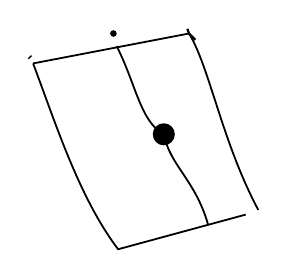
\begin{tikzpicture}[x=.2mm, y=-.2mm]
\draw[line width=.65pt](26,58)--(125,39)..controls(138,60)and(146,108)..(169,151);
\draw[line width=.65pt](26,58)..controls(40,95)and(55,143)..(80,176)--(161,154);
\draw[line width=.65pt](79,47)..controls(91,70)and(94,95)..(109,103)..controls(113,123)and(129,132)..(137,160);
\fill(109,103)circle(7);
\fill(77,39)circle(2.1);
\draw[line width=.8pt](124,36)--(125,39)--(129,43);
\draw[line width=.5pt](23,55)--(25,53);
\end{tikzpicture}}\end{minipage}}}\par\smallskip }
\end{GelfandAdjacentEvidence}

The number of flags --- a polynomial in $q$, whose degree depends on $n$.


\Needspace{7\baselineskip}
\begin{GelfandAdjacentEvidence}{GELFAND-P000366}{1}
\SourcePage{GELFAND-P000366}{25}
A coset class is determined by a partition $n=n_1+\dots+n_k$,
$u\in U$ --- an elem. of this class.
\begin{equation*}|P^{\boldsymbol{u}}|=P_{n_1,\dots, n_k}(q)\text{ --- a Hall polynomial}\end{equation*}
\uline{(the number of fixed points of this element).}
$u=1$ --- obtain the Poincare polynomial.
This allows one to determine the Poincare polynomial for any split group.
\Unclear{GELFAND-P000366}{allows-abbreviation}{The abbreviation after “This” has a first sign resembling Russian $\text{п}$, then a rounded sign and a z-like descending movement. “Pozv.” (“allows”) is provisionally rendered; the earlier reading “nazv.” is not secure. The Russian abbreviation remains unexpanded.}
\end{GelfandAdjacentEvidence}

\begin{center}\GelfandFitDiagram{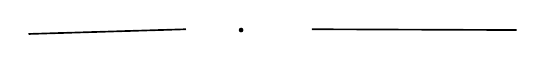
\begin{tikzpicture}[x=1mm, y=1mm]\draw[line width=.6pt](0,0)--(20,.6);\fill(27,.5)circle(.3);\draw[line width=.6pt](36,.6)--(62,.5);\end{tikzpicture}}\end{center}
J. A. Green, Trans. A. M. S., 1955 --- recommended.
\begin{center}\GelfandFitDiagram{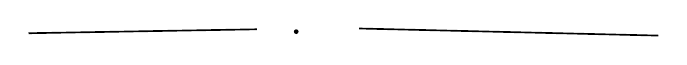
\begin{tikzpicture}[x=1mm, y=1mm]\draw[line width=.6pt](0,0)--(29,.5);\fill(34,.2)circle(.3);\draw[line width=.6pt](42,.6)--(80,-.3);\end{tikzpicture}}\end{center}
There are bounds on the dim. of the variety lying over a point here.
\begin{equation*}\pi:\bar R\longrightarrow R,\end{equation*}
\begin{center}\GelfandFitDiagram{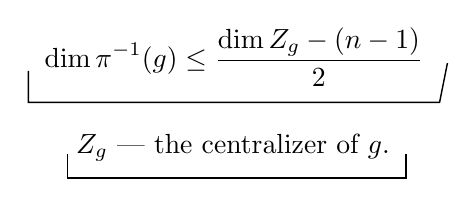
\begin{tikzpicture}
\node[inner sep=0](bound)at (0,0){$\displaystyle\dim\pi^{-1}(g)\le\frac{\dim Z_g-(n-1)}2$};
\draw[line width=.5pt]([xshift=-2mm,yshift=2mm]bound.south west)--([xshift=-2mm,yshift=-2mm]bound.south west)--([xshift=2mm,yshift=-2mm]bound.south east)--([xshift=3mm,yshift=3mm]bound.south east);
\node[anchor=north west, inner sep=0](centralizer)at ([xshift=4mm, yshift=-6mm]bound.south west){$Z_g$ --- the centralizer of $g$.};
\draw[line width=.5pt]([xshift=-1mm,yshift=1mm]centralizer.south west)--([xshift=-1mm,yshift=-2mm]centralizer.south west)--([xshift=2mm,yshift=-2mm]centralizer.south east)--([xshift=2mm,yshift=1mm]centralizer.south east);
\end{tikzpicture}}\end{center}



\begin{GelfandAdjacentEvidence}{GELFAND-P000366}{2}
\begin{center}\GelfandFitDiagram{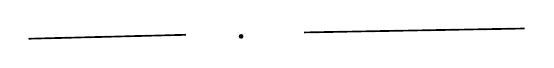
\begin{tikzpicture}[x=1mm, y=1mm]\draw[line width=.6pt](0,0)--(20,.5);\fill(27,.3)circle(.3);\draw[line width=.6pt](35,.8)--(63,1.3);\end{tikzpicture}}\end{center}
\uuline{B. Rosenfeld.}
On notes by \uline{Rego}, C. R., t. 272 (1971).
\sout{In the tang. space.}



\SourceFigure{GELFAND-P000366}{distribution-insertion}{\par\smallskip\centering{\color{black}\GelfandFitDiagram{\begin{minipage}{148mm}\raggedright \GelfandFitDiagram{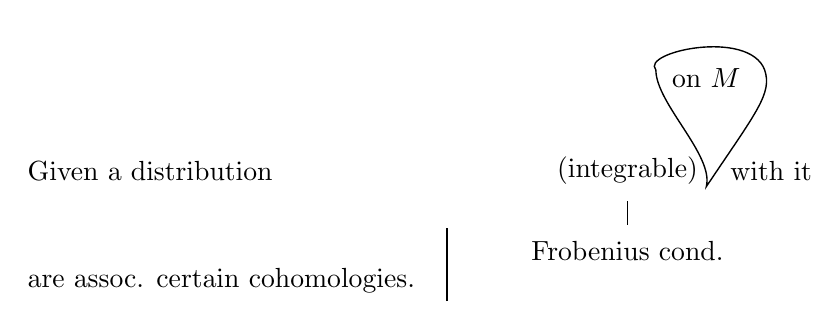
\begin{tikzpicture}
\node[anchor=west, inner sep=0](prefix)at (0,0){\uwave{Given a distribution}};
\node[anchor=west, inner sep=0](integrable)at ([xshift=36mm]prefix.east){(integrable)};
\node[anchor=west, inner sep=0]at ([xshift=4mm]integrable.east){with it};
\node[inner sep=0](insert)at ([xshift=1mm, yshift=10mm]integrable.north east){on $M$};
\draw[line width=.5pt]([xshift=-2mm,yshift=1mm]insert.west)..controls([xshift=-4mm,yshift=2mm]insert.north west)and([xshift=1mm,yshift=5mm]insert.north east)..([xshift=3mm,yshift=1mm]insert.east)..controls([xshift=4mm,yshift=-2mm]insert.east)and([xshift=2mm,yshift=-3mm]insert.south east)..([xshift=1mm,yshift=-2mm]integrable.east)..controls([xshift=2mm,yshift=2mm]integrable.east)and([xshift=-2mm,yshift=-2mm]insert.south west)..([xshift=-2mm,yshift=1mm]insert.west);
\draw[line width=.5pt]([yshift=-2mm]integrable.south)--([yshift=-5mm]integrable.south);
\node[anchor=north, inner sep=0]at ([yshift=-7mm]integrable.south){Frobenius cond.};
\node[anchor=north west, inner sep=0](cohomology)at ([yshift=-11mm]prefix.south west){are assoc. certain cohomologies.};
\draw[line width=.6pt]([xshift=4mm,yshift=-1mm]cohomology.south east)--([xshift=4mm,yshift=5mm]cohomology.north east);
\end{tikzpicture}}\end{minipage}}}\par\smallskip }
\end{GelfandAdjacentEvidence}
\begin{GelfandAdjacentEvidence}{GELFAND-P000366}{3}




\Unclear{GELFAND-P000366}{forms-insert-ending}{Above “diff. forms” a word is inserted, provisionally “kompleksno.”, rendered as “complex...”. The ending and contraction are doubtful; “kompleksna.”, “kompleksn.” and “kompleksa.” also remain candidates. Grammar has not selected a reading.\par\smallskip\centering{\color{black}\GelfandFitDiagram{\begin{minipage}{148mm}\raggedright \GelfandFitDiagram{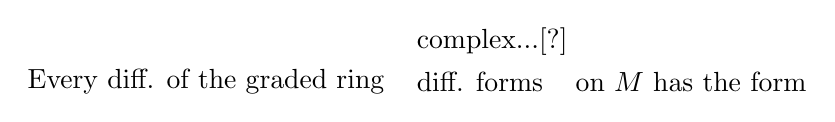
\begin{tikzpicture}
\node[anchor=west, inner sep=0](prefix)at (0,0){Every diff. of the graded ring};
\node[anchor=west, inner sep=0](forms)at ([xshift=4mm]prefix.east){diff. forms};
\node[anchor=south west, inner sep=0]at ([yshift=2mm]forms.north west){complex...[?]};
\node[anchor=west, inner sep=0]at ([xshift=4mm]forms.east){on $M$ has the form};
\end{tikzpicture}}\end{minipage}}}\par\smallskip }
\end{GelfandAdjacentEvidence}
\begin{GelfandAdjacentEvidence}{GELFAND-P000366}{4}

\begin{equation*}d_{L_1}+i_{L_2}\end{equation*}
($i_{L_2}$ --- interior multiplication by a vector-form).
\begin{center}\GelfandFitDiagram{\begin{tikzpicture}[x=1mm, y=1mm]\draw[line width=.45pt,dash pattern=on 2mm off 6mm](0,0)--(137,-2);\end{tikzpicture}}\end{center}
\begin{gather*}
\omega (X_1,\dots, X_q)\text{ --- a scalar form.}\\
L (X_1,\dots, X_p)\text{ --- a form (vector-valued).}\\
(i_L\omega)(X_1,\dots, X_{p+q-1})\quad\text{substitute and antisymmetrize.}\\
d_L\omega=(d\circ i_L+(-1)^p i_L\circ d)\omega.
\end{gather*}
$L$ --- a form of degree $0$ (vector field) --- $d_L$ --- the Lie derivative.
\sout{$d_L^2=0$}[?]
\Unclear{GELFAND-P000366}{integrable-cancel}{Before “integrability” a short formula is cancelled. $d_L^2=0$ is provisionally shown; the index and exponent on $d$ are hidden by overlapping strokes and not established securely.}
\end{GelfandAdjacentEvidence}

Integrability. (square $=0$)


\Needspace{7\baselineskip}
\begin{GelfandAdjacentEvidence}{GELFAND-P000367}{1}
\SourcePage{GELFAND-P000367}{unlabelled}
Prof. \uuline{Ptak}.
\begin{equation*}\dim E\le\infty,\qquad E\text{ with a norm}.\end{equation*}
\Unclear{GELFAND-P000367}{dimension-sign}{Between $\dim E$ and $\infty$ several oblique and horizontal strokes overlap. $\le$ is provisionally shown; $<$ and $\ne$ remain candidates.}
\end{GelfandAdjacentEvidence}
\begin{GelfandAdjacentEvidence}{GELFAND-P000367}{2}

$q$ --- an exponent (crit.) if
\begin{equation*}1^\circ.\quad A\in L (E),\quad1=|A|=|A^{\boldsymbol{q}}|\Rightarrow|A|_\sigma=1\quad\text{(sp. radius)}.\end{equation*}
\Unclear{GELFAND-P000367}{a-exponent}{The exponent on the second $A$ is heavily thickened or rewritten. $q$ is shown provisionally; the earlier exponent is unestablished.}
\end{GelfandAdjacentEvidence}
\begin{GelfandAdjacentEvidence}{GELFAND-P000367}{3}

\begin{equation*}2^\circ.\quad\exists B,\quad1=|B|=|B^{q-1}|,\quad\text{but }|B|_\sigma<1.\end{equation*}
\begin{equation*}\begin{aligned}\ell^\infty\quad&|x|=\max|x_i|,\\\ell_1\quad&\sum|x_i|,\end{aligned}\qquad q (n)=n^2-n+1.\end{equation*}
\begin{equation*}\ell_2\qquad q (n)=n.\end{equation*}
There exists a $2$-dim. space in which $q=\infty$.
(The norm gives poor estimates of convergence; eigenvalues are needed).



\SourceFigure{GELFAND-P000367}{danzer-diagram}{\par\smallskip\centering{\color{black}\GelfandFitDiagram{\begin{minipage}{68mm}\raggedright \GelfandFitDiagram{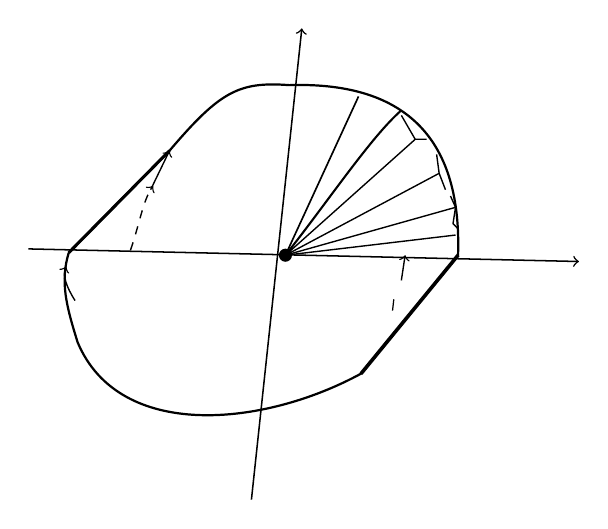
\begin{tikzpicture}[x=.16mm, y=-.16mm]
\draw[line width=.8pt](45,193)--(125,112)..controls(165,65)and(180,57)..(220,60)..controls(315,57)and(357,105)..(354,195)--(277,289)..controls(200,331)and(85,343)..(52,264)..controls(43,235)and(38,216)..(45,193);
\draw[line width=1.1pt](45,193)--(125,112);
\draw[line width=1.3pt](354,195)--(277,289);
\draw[line width=.55pt,->](190,389)--(230,15);
\draw[line width=.55pt,->](13,190)--(450,200);
\fill(217,195)circle(5.2);
\draw[line width=.6pt](217,195)--(275,69);
\draw[line width=.75pt](217,195)..controls(251,152)and(285,101)..(309,80);
\draw[line width=.5pt](217,195)--(320,103);
\draw[line width=.5pt](217,195)--(339,130);
\draw[line width=.5pt](217,195)--(352,157);
\draw[line width=.5pt](217,195)--(352,179);
\draw[line width=.5pt](309,84)--(320,103)--(329,103);
\draw[line width=.5pt](337,115)--(339,130)--(344,143);
\draw[line width=.5pt](348,148)--(352,157)--(350,170)--(354,174);
\draw[line width=.5pt,dashed,->](94,191)..controls(101,171)and(104,151)..(112,140);
\draw[line width=.5pt,->](110,143)--(125,112);
\draw[line width=.5pt,->](50,231)..controls(43,220)and(40,211)..(43,204);
\draw[line width=.5pt,->](309,215)--(312,195);
\draw[line width=.45pt](303,230)--(302,239);
\end{tikzpicture}}\end{minipage}}}\par\smallskip }
\end{GelfandAdjacentEvidence}
\begin{GelfandAdjacentEvidence}{GELFAND-P000367}{4}

$A$ --- rotation by a small angle (Danzer's example).
$\ell_p$ --- unknown whether it exists, except for $p=2^m$.
\uline{A useful problem for computational mathematics.}
\begin{equation*}M (n)=\min\text{ over all ban. }\le n.\end{equation*}
\Unclear{GELFAND-P000367}{banach-overwritten}{The abbreviation after “over all” is provisionally shown as “ban.”. Its middle letters are heavily thickened and rewritten; earlier strokes are not separated. The abbreviation is not expanded.}
\end{GelfandAdjacentEvidence}
\begin{GelfandAdjacentEvidence}{GELFAND-P000367}{5}

$\exists$ those for which $<n$!
There exists a seq. $M (n_k)\sim\sqrt{n_k}$.
It is unknown whether $\liminf M (n)=\infty$ is true.
\begin{equation*}\ell_4^2\underset{\ell_1}{\oplus}\ell_8^2\end{equation*}



\Unclear{GELFAND-P000367}{dimension-insert}{Above the cancelled earlier word is the legible outlined insertion “here”. The earlier “eto” (“this”) is shown provisionally; the covered letters do not establish its complete reading.\par\smallskip\centering{\color{black}\GelfandFitDiagram{\begin{minipage}{148mm}\raggedright \GelfandFitDiagram{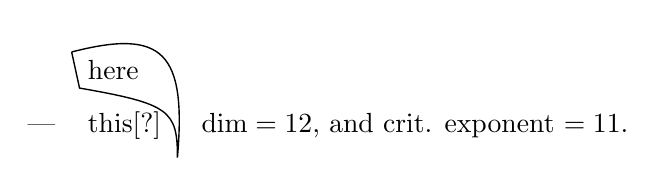
\begin{tikzpicture}
\node[anchor=west, inner sep=0](dash)at (0,0){---};
\node[anchor=west, inner sep=0](old)at ([xshift=4mm]dash.east){\sout{this}[?]};
\node[anchor=south west, inner sep=0](insert)at ([yshift=4mm]old.north west){here};
\draw[line width=.5pt]([xshift=-2mm,yshift=1mm]insert.north west)..controls([xshift=3mm,yshift=4mm]insert.north east)and([xshift=6mm,yshift=1mm]insert.north east)..([xshift=2mm,yshift=-4mm]old.east)..controls([xshift=2mm,yshift=2mm]old.east)and([xshift=1mm,yshift=1mm]old.north east)..([xshift=-1mm,yshift=-1mm]insert.south west)--([xshift=-2mm,yshift=1mm]insert.north west);
\node[anchor=west, inner sep=0]at ([xshift=5mm]old.east){$\dim=12$, and crit. exponent $=11$.};
\end{tikzpicture}}\end{minipage}}}\par\smallskip }
\end{GelfandAdjacentEvidence}

\begin{equation*}C (E, r,\rho)=\max\{|T^r|,\ |T|\le1,\ |T|_\sigma\le\rho\}.\end{equation*}
\begin{center}\GelfandFitDiagram{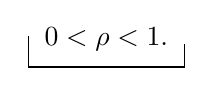
\begin{tikzpicture}
\node[inner sep=0](rho)at (0,0){$0<\rho<1$.};
\draw[line width=.5pt]([xshift=-2mm,yshift=2mm]rho.south west)--([xshift=-2mm,yshift=-2mm]rho.south west)--([xshift=2mm,yshift=-2mm]rho.south east)--([xshift=2mm,yshift=1mm]rho.south east);
\end{tikzpicture}}\end{center}



\begin{center}\GelfandFitDiagram{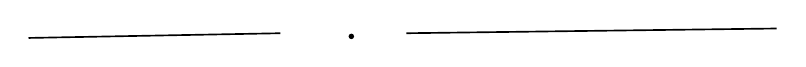
\begin{tikzpicture}[x=1mm, y=1mm]\draw[line width=.6pt](0,0)--(32,.6);\fill(41,.2)circle(.35);\draw[line width=.6pt](48,.6)--(95,1.2);\end{tikzpicture}}\end{center}


\Needspace{7\baselineskip}
\SourcePage{GELFAND-P000368}{26}
\underline{I. M. Gelfand.}

\begin{GelfandAdjacentEvidence}{GELFAND-P000368}{1}
C Radon formula over a finite field.
\Unclear{GELFAND-P000368}{radon-prefix}{Before “formula” is a separate C-shaped sign, shown as “C”. Its meaning and relation to the following abbreviation are unestablished.}
\end{GelfandAdjacentEvidence}

Over $F_q$ an $n$-dim. space. $(x_1,\dots, x_n)$.
\hfill $q^n$ points.

\begin{GelfandAdjacentEvidence}{GELFAND-P000368}{2}
Integrals over all planes are known.
\begin{equation*}\varphi (p)=\int_{x\in p}f (x)\quad\text{(sum)}.\end{equation*}
$p$ --- a plane.



\SourceFigure{GELFAND-P000368}{first-count-caption}{\par\smallskip\centering{\color{black}\GelfandFitDiagram{\begin{minipage}{148mm}\raggedright \GelfandFitDiagram{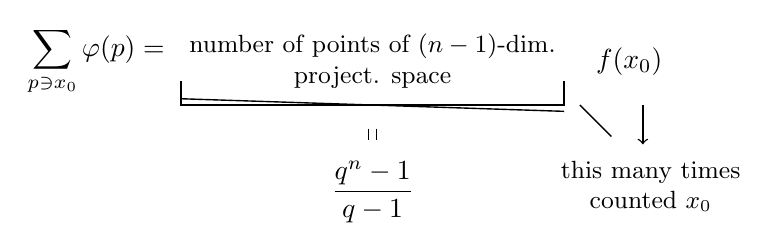
\begin{tikzpicture}[x=1mm, y=1mm]
\node[anchor=west, inner sep=0](sum)at (0,0){$\displaystyle\sum_{p\ni x_0}\varphi (p)=$};
\node[anchor=west, inner sep=0](count)at ([xshift=3mm]sum.east){\small\shortstack{number of points of $(n-1)$-dim.\\project. space}};
\node[anchor=west, inner sep=0](factor)at ([xshift=5mm]count.east){$f (x_0)$};
\draw[line width=.5pt]([xshift=-1mm,yshift=1mm]count.south west)--([xshift=-1mm,yshift=-2mm]count.south west)--([xshift=1mm,yshift=-2mm]count.south east)--([xshift=1mm,yshift=1mm]count.south east);
\draw[line width=.5pt]([xshift=-1mm,yshift=-1.2mm]count.south west)--([xshift=1mm,yshift=-2.8mm]count.south east);
\draw[line width=.45pt]([xshift=-.5mm,yshift=-5mm]count.south)--([xshift=-.5mm,yshift=-6.5mm]count.south);
\draw[line width=.45pt]([xshift=.5mm,yshift=-5mm]count.south)--([xshift=.5mm,yshift=-6.5mm]count.south);
\node[inner sep=0](alpha)at ([yshift=-13mm]count.south){$\displaystyle\frac{q^n-1}{q-1}$};
\draw[line width=.5pt]([xshift=3mm,yshift=-2mm]count.south east)--([xshift=7mm,yshift=-6mm]count.south east);
\draw[line width=.5pt,->]([xshift=11mm,yshift=-2mm]count.south east)--([xshift=11mm,yshift=-7mm]count.south east);
\node[anchor=north, inner sep=0]at ([xshift=12mm, yshift=-9mm]count.south east){\small\shortstack{this many times\\counted $x_0$}};
\end{tikzpicture}}\end{minipage}}}\par\smallskip }
\end{GelfandAdjacentEvidence}
\begin{GelfandAdjacentEvidence}{GELFAND-P000368}{3}

\begin{equation*}+\frac{q^{n-1}-1}{q-1}\sum_{x\ne x_0}f (x).\end{equation*}



\Unclear{GELFAND-P000368}{cancelled-term-symbol}{In the cancelled term the angular sign before $(x_0)$ is provisionally shown as $A$. $f$ remains a candidate; the crossing cancellation strokes prevent a unique reading. The entire term is cancelled; an equals sign follows it.\par\smallskip\centering{\color{black}\GelfandFitDiagram{\begin{minipage}{148mm}\raggedright \GelfandFitDiagram{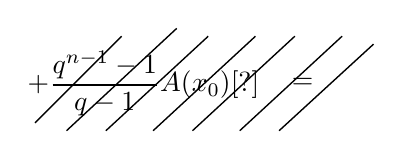
\begin{tikzpicture}[x=1mm, y=1mm]
\node[anchor=west, inner sep=0](old)at (0,0){$\displaystyle+\frac{q^{n-1}-1}{q-1}A (x_0)$[?]};
\draw[line width=.5pt]([xshift=1mm,yshift=-5mm]old.west)--([xshift=12mm,yshift=6mm]old.west);
\draw[line width=.5pt]([xshift=5mm,yshift=-6mm]old.west)--([xshift=19mm,yshift=7mm]old.west);
\draw[line width=.5pt]([xshift=10mm,yshift=-6mm]old.west)--([xshift=23mm,yshift=6mm]old.west);
\draw[line width=.5pt]([xshift=16mm,yshift=-6mm]old.west)--([xshift=29mm,yshift=6mm]old.west);
\draw[line width=.5pt]([xshift=21mm,yshift=-6mm]old.west)--([xshift=34mm,yshift=6mm]old.west);
\draw[line width=.5pt]([xshift=27mm,yshift=-6mm]old.west)--([xshift=40mm,yshift=6mm]old.west);
\draw[line width=.5pt]([xshift=32mm,yshift=-6mm]old.west)--([xshift=44mm,yshift=5mm]old.west);
\node[anchor=west, inner sep=0]at ([xshift=4mm]old.east){$=$};
\end{tikzpicture}}\end{minipage}}}\par\smallskip }
\end{GelfandAdjacentEvidence}
\begin{GelfandAdjacentEvidence}{GELFAND-P000368}{4}

\begin{equation*}\sum_x f (x)=\sum_{p\parallel p_0}\varphi (p)\quad\text{\sout{[?]}}\quad\equiv C.\end{equation*}
\Incomplete{GELFAND-P000368}{parallel-condition}{Between the sum over $p\parallel p_0$ and $\equiv C$ several signs are cancelled. Their reading is unestablished.}
\end{GelfandAdjacentEvidence}
\begin{GelfandAdjacentEvidence}{GELFAND-P000368}{5}

(does not depend on $p_0$) --- a cond. on $\varphi (p)$ --- an analogue of the Paley--Wiener theorem.



\SourceFigure{GELFAND-P000368}{known-sum-caption}{The sum $\sum_x f (x)$ is circled; beneath it “$C$ --- known.” is underlined. The lower index has overlapping strokes and a small loop; $x$ is retained provisionally.\par\smallskip\centering{\color{black}\GelfandFitDiagram{\begin{minipage}{148mm}\raggedright \GelfandFitDiagram{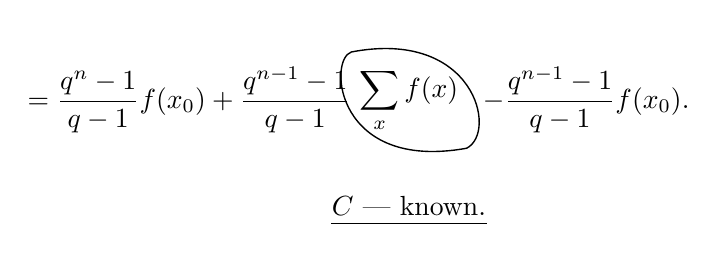
\begin{tikzpicture}[x=1mm, y=1mm]
\node[anchor=west, inner sep=0](left)at (0,0){$\displaystyle=\frac{q^n-1}{q-1}f (x_0)+\frac{q^{n-1}-1}{q-1}$};
\node[anchor=west, inner sep=0](total)at ([xshift=1mm]left.east){$\displaystyle\sum_x f (x)$};
\node[anchor=west, inner sep=0]at ([xshift=3mm]total.east){$\displaystyle-\frac{q^{n-1}-1}{q-1}f (x_0). $};
\draw[line width=.5pt]([xshift=-1mm,yshift=2mm]total.north west)..controls([xshift=2mm,yshift=5mm]total.north east)and([xshift=5mm,yshift=0mm]total.south east)..([xshift=1mm,yshift=-2mm]total.south east)..controls([xshift=-3mm,yshift=-5mm]total.south west)and([xshift=-4mm,yshift=1mm]total.north west)..([xshift=-1mm,yshift=2mm]total.north west);
\node[anchor=north, inner sep=0](known)at ([yshift=-8mm]total.south){$C$ --- known.};
\draw[line width=.5pt]([yshift=-1mm]known.south west)--([yshift=-1mm]known.south east);
\end{tikzpicture}}\end{minipage}}}\par\smallskip }
\end{GelfandAdjacentEvidence}


\uuline{Rota} --- as $q\to1$ one obtains a passage to simple theorems.
$C_k^n (q)$ --- the number of $k$-dim. subspaces of an $n$-dim. space.
\begin{equation*}\lim_{q\to1}C_k^n (q)=C_k^n\text{ --- \underline{combinations}}.\end{equation*}


\Needspace{7\baselineskip}
\SourcePage{GELFAND-P000369}{unlabelled}
\uuline{Kirillov.}

\begin{GelfandAdjacentEvidence}{GELFAND-P000369}{1}
Consider an arbitrary generalized function $A$ on a manifold $M$ (e.g. $R^n$).
For it a wave front is defined
\begin{equation*}WF (A)\subset T^*M.\end{equation*}
A smooth function --- zero wave front (empty).
Let $\xi\in T^*M$.
\begin{gather*}\xi\notin WF (A),\quad\text{if}\\
\langle A,\varphi e^{it\boldsymbol{\psi}}\rangle=o (t^{-n}),\quad\forall n\quad\text{as }t\to+\infty.\end{gather*}
\Unclear{GELFAND-P000369}{phase-reinforced}{The phase sign after $it$ is heavily thickened or rewritten. $\psi$ is shown provisionally; the earlier strokes are not separated.}
\end{GelfandAdjacentEvidence}

(here $d\psi=\xi$ at the point $\pi_\xi$ and $\varphi\in C_0^\infty$ is arbitrary).

It is convenient to study functions for which the wave front $\in$ a Lagr. manifold.
\begin{center}\GelfandFitDiagram{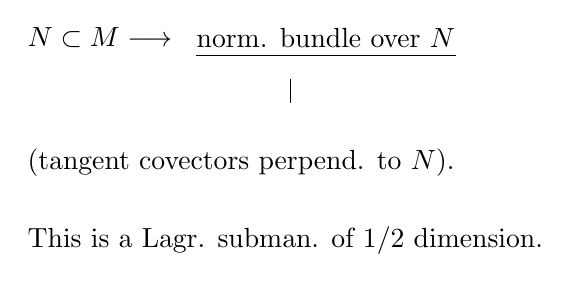
\begin{tikzpicture}[x=1mm, y=1mm]
\node[anchor=west, inner sep=0](start)at (0,0){$N\subset M\longrightarrow$};
\node[anchor=west, inner sep=0](normal)at ([xshift=3mm]start.east){norm. bundle over $N$};
\draw[line width=.55pt]([yshift=-1mm]normal.south west)--([yshift=-1mm]normal.south east);
\draw[line width=.5pt]([xshift=12mm,yshift=-4mm]normal.south west)--([xshift=12mm,yshift=-7mm]normal.south west);
\node[anchor=north west, inner sep=0]at (0,-14){(tangent covectors perpend. to $N$).};
\node[anchor=north west, inner sep=0]at (0,-24){This is a Lagr. subman. of $1/2$ dimension.};
\end{tikzpicture}}\end{center}



\begin{GelfandAdjacentEvidence}{GELFAND-P000369}{2}

\sout{[?]} P. D. O. --- a generalized function on $M\times M$ (kernel) with a wave front constructed in this way from the diagonal.
\Unclear{GELFAND-P000369}{pdo-cancel}{Before “P. D. O.” a short word is heavily cancelled. “Napr.” (“e.g.”) remains a candidate; the complete reading is unestablished.}
\end{GelfandAdjacentEvidence}
\begin{GelfandAdjacentEvidence}{GELFAND-P000369}{3}

\begin{center}\GelfandFitDiagram{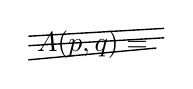
\begin{tikzpicture}
\node[inner sep=0](old)at (0,0){$A (p, q)=$};
\draw[line width=.5pt]([xshift=-1mm,yshift=1mm]old.west)--([xshift=2mm,yshift=2mm]old.east);
\draw[line width=.5pt]([xshift=-1mm,yshift=-.2mm]old.west)--([xshift=2mm,yshift=.8mm]old.east);
\draw[line width=.5pt]([xshift=-1mm,yshift=-2mm]old.west)--([xshift=1mm,yshift=-.5mm]old.east);
\end{tikzpicture}}\end{center}
\begin{equation*}\langle A\mathord{[?]}u\rangle=\int e^{i\psi (x,\xi)}a (x,\xi)u (x)\, dx\, d\xi.\end{equation*}
\Unclear{GELFAND-P000369}{pairing-prefix}{Between $A$ and $u$ is a reinforced vertical sign with an upper loop or dot and a lower bend; beside it is a separate lower stroke. $i$, a comma, a semicolon and a cancelled sign remain possible readings.}
\end{GelfandAdjacentEvidence}

(Value of $A$ on the test function $u$).

\begin{GelfandAdjacentEvidence}{GELFAND-P000369}{4}
Every $A$ \sout{[?]} with wave front defined this way is given by this formula.
\Incomplete{GELFAND-P000369}{lower-cancel}{After “Every $A$” a separate sign is heavily cancelled. Its reading is unestablished.}
\end{GelfandAdjacentEvidence}
\begin{GelfandAdjacentEvidence}{GELFAND-P000369}{5}




\Unclear{GELFAND-P000369}{wavefront-prefix}{After “Wave front” a rounded sign is cancelled. $\varphi$ is shown provisionally; another reading is not excluded. The following $\in\Lambda$ is retained separately from the cancellation.\par\smallskip\centering{\color{black}\GelfandFitDiagram{\begin{minipage}{148mm}\raggedright \begin{equation*}\text{Wave front }\text{\sout{$\varphi$}[?]}\in\Lambda=\left\{\underset{\substack{x\in M\\\xi\in T^*M}}{x,\xi}\;\middle|\; d\psi=\xi\, dx\right\}.\end{equation*}\end{minipage}}}\par\smallskip }
\end{GelfandAdjacentEvidence}




\begin{center}\GelfandFitDiagram{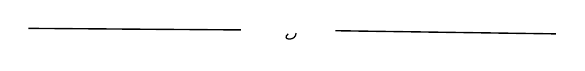
\begin{tikzpicture}[x=1mm, y=1mm]
\draw[line width=.5pt](0,0)--(27,-.2);
\draw[line width=.45pt](33,-.7)..controls(32,-1.5)and(34,-1.7)..(34,-.6);
\draw[line width=.5pt](39,-.3)--(67,-.7);
\end{tikzpicture}}\end{center}


\Needspace{7\baselineskip}
\begin{GelfandAdjacentEvidence}{GELFAND-P000370}{1}
\SourcePage{GELFAND-P000370}{27}
20/$\overline{\underline{\mathrm{IX}}}$ \raisebox{1.5mm}{\rule{.3pt}{1.2mm}}
\Unclear{GELFAND-P000370}{heading-date-tail}{To the right of $20/\mathrm{IX}$ is a separate short vertical 1-like stroke. Its meaning is unestablished.}
\end{GelfandAdjacentEvidence}
\begin{GelfandAdjacentEvidence}{GELFAND-P000370}{2}




\SourceFigure{GELFAND-P000370}{guest-heading-tab}{\par\smallskip\centering{\color{black}\GelfandFitDiagram{\begin{minipage}{148mm}\raggedright \GelfandFitDiagram{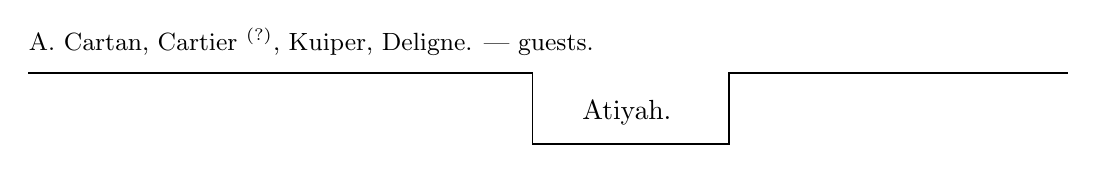
\begin{tikzpicture}[x=1mm, y=1mm]
\node[anchor=west, inner sep=0](guests)at (0,0){\small A. Cartan, Cartier $^{(?)}$, Kuiper, Deligne. --- guests.};
\node[inner sep=0](atiyah)at (76,-9){Atiyah.};
\draw[line width=.55pt](0,-4)--(64,-4)--(64,-13)--(89,-13)--(89,-4)--(132,-4);
\end{tikzpicture}}\end{minipage}}}\par\smallskip }
\end{GelfandAdjacentEvidence}


\begin{GelfandAdjacentEvidence}{GELFAND-P000370}{3}
\underline{I. Bernstein.} on work of Godbillon, Vey. Comptes rendus.
$M$ --- a compact manifold.
On $M$ is given a form $\omega$ (a \underline{foliation} $S$ of codim. $1$), which is integrable.
\begin{equation*}d\omega=\omega\wedge\omega_1.\end{equation*}
--- \sout{[?]}
\Incomplete{GELFAND-P000370}{integrable-cancel}{After the formula an earlier word is heavily cancelled; its reading is unestablished.}
\end{GelfandAdjacentEvidence}
\begin{GelfandAdjacentEvidence}{GELFAND-P000370}{4}

\sout{[?]} To it is associated $\alpha_s\in H^3(M, R)$, it
\Incomplete{GELFAND-P000370}{class-cancelled-clause}{Before “To it is associated” an entire phrase is heavily cancelled; its reading is unestablished.}
\end{GelfandAdjacentEvidence}
\begin{GelfandAdjacentEvidence}{GELFAND-P000370}{5}

\sout{[?]} $=0$ if this is a fibration and is stable under deformations,
\Incomplete{GELFAND-P000370}{zero-cancel}{After “it” and before $=0$ a short word is heavily cancelled. No confident reading of its letters is established.}
\end{GelfandAdjacentEvidence}
\begin{GelfandAdjacentEvidence}{GELFAND-P000370}{6}

\sout{[?]} $\ne0$.
\Incomplete{GELFAND-P000370}{deformation-cancel}{Between “under deformations” and $\ne0$ a short word is crossed out; its reading is unestablished.}
\end{GelfandAdjacentEvidence}


\begin{GelfandAdjacentEvidence}{GELFAND-P000370}{7}
Construction: there exist forms $\omega_1$, $\omega_2$:
\begin{gather*}d\omega=\omega\wedge\omega_1;\\d\omega_1=\omega\wedge\omega_2.\end{gather*}
\begin{center}\GelfandFitDiagram{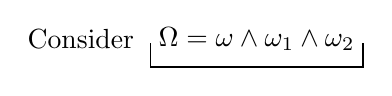
\begin{tikzpicture}
\node[anchor=west, inner sep=0](consider)at (0,0){Consider};
\node[anchor=west, inner sep=0](omega)at ([xshift=3mm]consider.east){$\Omega=\omega\wedge\omega_1\wedge\omega_2$};
\draw[line width=.5pt]([xshift=-1mm,yshift=1mm]omega.south west)--([xshift=-1mm,yshift=-2mm]omega.south west)--([xshift=1mm,yshift=-2mm]omega.south east)--([xshift=1mm,yshift=1mm]omega.south east);
\end{tikzpicture}}\end{center}
--- closed, and the cohom. class does not depend on the choice of $\omega_1$ and $\omega_2$.
There is a connection with the cohomology of algebras.




\Unclear{GELFAND-P000370}{quotient-end}{After $SL (2, R)$ is a reinforced M-like sign. $M$ is shown provisionally; the overlapping strokes are unestablished.}
\end{GelfandAdjacentEvidence}
\begin{GelfandAdjacentEvidence}{GELFAND-P000370}{8}

\SourceFigure{GELFAND-P000370}{quotient-annotations}{\par\smallskip\centering{\color{black}\GelfandFitDiagram{\begin{minipage}{148mm}\raggedright \GelfandFitDiagram{\begin{tikzpicture}[x=1mm, y=1mm]
\draw[line width=.6pt](0,7)--(0,-59);
\node[anchor=west, inner sep=0]at (5,0){\underline{Example:}};
\node[anchor=west, inner sep=0]at (35,0){$SL (2, R)\,\boldsymbol M$[?]};
\draw[line width=.75pt](30,5)--(39,-7);
\node[inner sep=0](gamma)at (30,-11){$\Gamma$};
\draw[line width=.5pt](26,-16)..controls(29,-18)and(33,-18)..(35,-16);
\node[anchor=west, inner sep=0]at (22,-23){discr. subgr.};
\node[anchor=west, inner sep=0]at (76,-12){--- compact.};
\node[anchor=west, inner sep=0]at (8,-38){and $\begin{pmatrix}a&0\\c&b\end{pmatrix}$};
\node[anchor=west, inner sep=0]at (45,-35){dense trajectories ---};
\node[anchor=west, inner sep=0]at (74,-44){--- always.};
\node[anchor=west, inner sep=0]at (22,-56){Then it is $\ne0$.};
\end{tikzpicture}}\end{minipage}}}\par\smallskip }
\end{GelfandAdjacentEvidence}


Foliation:
\begin{center}\GelfandFitDiagram{\begin{tikzpicture}
\node[anchor=west, inner sep=0](maps)at (0,0){$\begin{gathered}\varphi_i: U_i\longrightarrow R,\\\varphi_j\varphi_i: U_i\cap U_j\longrightarrow R.\end{gathered}$};
\node[anchor=west, inner sep=0](interval)at ([xshift=8mm]maps.east){\shortstack{on an interval\\of the line}};
\draw[line width=.5pt]([xshift=-2mm,yshift=2mm]interval.north west)--([xshift=2mm,yshift=2mm]interval.north east);
\draw[line width=.5pt]([xshift=-2mm,yshift=-2mm]interval.south west)--([xshift=2mm,yshift=-2mm]interval.south east);
\draw[line width=.6pt]([xshift=2mm,yshift=12mm]interval.north east)--([xshift=2mm,yshift=-12mm]interval.south east);
\end{tikzpicture}}\end{center}



Since the leaves are the same, one obtains $\Psi_{ij}: R\to R$ (an interval).
If $\Psi_{ij}\in$ a group, then a cocycle with coeff. in the group $\longrightarrow$ a bundle and from it cohomology classes. But this is a pseudogroup.
But consider a Lie algebra isom. to $W_1$ --- formal vector fields on the line, $f (x)\frac{d}{dx}$.
They are $=0$, except there exists $H^3(W_1, R)=R$. This is precisely that class.

\begin{GelfandAdjacentEvidence}{GELFAND-P000370}{9}
\uuline{Atiyah.}
\underline{On the spectrum of a selfadj. elliptic operator.}
$X$ --- a compact manifold,
$D$ --- an elliptic diff. operator, selfadj. $D^*=D$.
Discr. spectrum; eigenvalues are divided into positive and negative.
Let $D=D_t$, $t$ --- a param.; the spectrum changes with $t$.



\SourceFigure{GELFAND-P000370}{spectrum-sketch}{An inclined nearly vertical line with twelve distinguishable transverse strokes of different lengths and short overlapping strokes. One stroke in the middle is thickened. Exact intervals and separation of all overlapping strokes are unestablished; there are no numerical labels.\par\smallskip\centering{\color{black}\GelfandFitDiagram{\begin{minipage}{68mm}\raggedright \GelfandFitDiagram{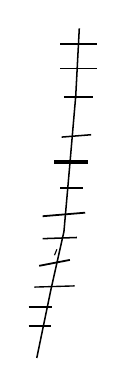
\begin{tikzpicture}[x=.15mm, y=-.15mm]
\draw[line width=.55pt](65,27)--(62,84)--(57,142)--(52,199)--(41,248)--(29,306);
\draw[line width=.55pt](49,40)--(80,40);
\draw[line width=.55pt](49,61)--(80,61);
\draw[line width=.5pt](52,85)--(77,85);
\draw[line width=.55pt](50,119)--(75,117);
\draw[line width=1.35pt](44,140)--(72,140);
\draw[line width=.6pt](49,162)--(68,162);
\draw[line width=.65pt](34,186)--(70,183);
\draw[line width=.55pt](34,205)--(63,204);
\draw[line width=.65pt](31,228)--(57,223);
\draw[line width=.5pt](27,246)--(61,245);
\draw[line width=.55pt](22,263)--(42,263);
\draw[line width=.6pt](22,279)--(41,279);
\draw[line width=.4pt](46,214)--(44,219);
\end{tikzpicture}}\end{minipage}}}\par\smallskip }
\end{GelfandAdjacentEvidence}
\begin{GelfandAdjacentEvidence}{GELFAND-P000370}{10}

Let $\underline{D_{t+1}=D_t}$ --- periodicity, or



\Unclear{GELFAND-P000370}{unitary-overwrite}{The first $U$ stands on the main line; a small cancelled earlier sign is above and to its right. “na” remains a candidate; the exact reading is unestablished. The order of insertion is undetermined.\par\smallskip\centering{\color{black}\GelfandFitDiagram{\begin{minipage}{148mm}\raggedright \GelfandFitDiagram{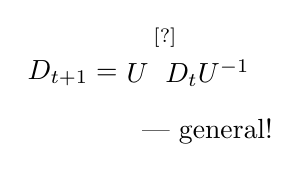
\begin{tikzpicture}
\node[anchor=west, inner sep=0](left)at (0,0){$D_{t+1}=$};
\node[anchor=west, inner sep=0](unitary)at ([xshift=1mm]left.east){$U$};
\node[anchor=west, inner sep=0](right)at ([xshift=2mm]unitary.east){$D_tU^{-1}$};
\node[anchor=south west, inner sep=0](old)at ([xshift=.5mm, yshift=2mm]unitary.north east){\scriptsize\sout{[?]}};
\node[anchor=north, inner sep=0]at ([yshift=-4mm]right.south){--- general!};
\end{tikzpicture}}\end{minipage}}}\par\smallskip }
\end{GelfandAdjacentEvidence}

$(U=\mathrm{const})$.


\Needspace{7\baselineskip}
\begin{GelfandAdjacentEvidence}{GELFAND-P000371}{1}
\SourcePage{GELFAND-P000371}{unlabelled}
\begin{equation*}\operatorname{Spec}D_{t+1}=\operatorname{Spec}D_t.\end{equation*}
The spectrum moves (eigenvalues may shift by $q$[?]).
\Unclear{GELFAND-P000371}{shift-size}{After “by” is a reinforced q-like sign. $q$ is shown provisionally; a question mark remains a candidate.}
\end{GelfandAdjacentEvidence}
\begin{GelfandAdjacentEvidence}{GELFAND-P000371}{2}

One can define an \uuline{integer} characterizing this shift.
(Place an observer at $0$ and see what mass has passed to the left and to the right.)



\SourceFigure{GELFAND-P000371}{spectrum-graphs}{Upper drawing: axes $\lambda, t$, marks $0,1$, two verticals and three wavy curves. Thick dots occur at endpoints and on the axis; the lower right dot has a light centre. Below are six distinguishable inclined segments between nearly vertical lines. Exact separation of overlapping strokes and joins is unestablished.\par\smallskip\centering{\color{black}\GelfandFitDiagram{\begin{minipage}{68mm}\raggedright \GelfandFitDiagram{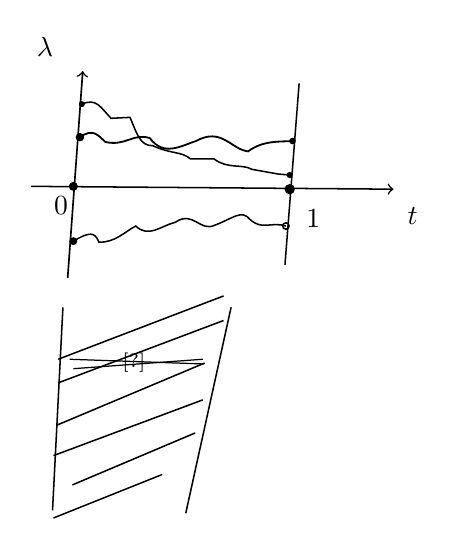
\begin{tikzpicture}[x=.12mm, y=-.12mm]
\draw[line width=.55pt,->](16,182)--(400,185);
\draw[line width=.6pt,->](55,279)--(71,60);
\draw[line width=.55pt](300,73)--(285,265);
\node at (31,34){$\lambda$};\node at (420,213){$t$};\node at (48,202){$0$};\node at (315,216){$1$};
\draw[line width=.55pt](70,95)..controls(86,88)and(90,99)..(101,110)--(121,109)..controls(129,128)and(132,139)..(145,139)..controls(165,148)and(176,145)..(185,153)--(210,153)..controls(224,164)and(240,158)..(250,164)--(278,169)--(290,170);
\draw[line width=.65pt](68,130)..controls(82,120)and(87,128)..(95,135)..controls(116,140)and(125,125)..(142,131)..controls(157,151)and(175,139)..(191,134)..controls(218,119)and(228,143)..(246,145)..controls(262,133)and(280,135)..(293,134);
\draw[line width=.55pt](61,240)..controls(78,230)and(84,230)..(88,241)..controls(105,242)and(117,229)..(127,224)..controls(141,237)and(153,224)..(169,220)..controls(188,207)and(195,231)..(211,223)..controls(230,216)and(239,206)..(248,217)..controls(261,229)and(270,219)..(286,224);
\fill(70,95)circle(3.2);\fill(68,130)circle(4.5);\fill(61,240)circle(4.2);
\fill(290,170)circle(3.3);\fill(293,134)circle(3.5);\draw[line width=.55pt](286,224)circle(3.4);
\fill(61,182)circle(4.8);\fill(290,185)circle(5.5);
\draw[line width=.55pt](50,310)--(39,525);
\draw[line width=.55pt](228,310)--(180,528);
\draw[line width=.55pt](45,365)--(220,298);
\draw[line width=.55pt](45,390)--(220,324);
\draw[line width=.55pt](43,435)--(200,369);
\draw[line width=.55pt](40,467)--(198,408);
\draw[line width=.55pt](60,498)--(190,443);
\draw[line width=.55pt](40,533)--(155,487);
\node[inner sep=0]at (125,369){\scriptsize\sout{[?]}};
\draw[line width=.45pt](57,365)--(199,370);
\draw[line width=.45pt](61,375)--(198,365);
\end{tikzpicture}}\end{minipage}}}\par\smallskip }
\end{GelfandAdjacentEvidence}
\begin{GelfandAdjacentEvidence}{GELFAND-P000371}{3}

\Incomplete{GELFAND-P000371}{graphs-cancelled-caption}{In the middle of the lower drawing a short caption is cancelled, distinct from the inclined lines. No complete word or formula has been recovered.}
\end{GelfandAdjacentEvidence}


\uuline{Example.} Spectral flow $\in Z$.
\begin{equation*}X\text{ --- a circle,}\qquad D_t=-i\frac{d}{dx}+t,\qquad Uf=e^{ix}f.\end{equation*}
\uwave{Flow} $=\pm1$ $(n\to n+1)$.
\uwave{This is a top. invariant under deformations of the family.}
\uuline{Problem:} compute spectral flow from the geom. data of the problem: manifold, operator, $U$.
Connected with the index.
Let the operator $D$ be of $1$ st order (a system).
Consider
\begin{center}\GelfandFitDiagram{\begin{tikzpicture}
\node[anchor=west, inner sep=0](P)at (0,0){$P$};
\node[anchor=west, inner sep=0](op)at (P.east){$\displaystyle\equiv D_t+\frac{\partial}{\partial t}$};
\draw[line width=.55pt]([yshift=1mm]op.south west)--([yshift=-4mm]op.south west)--([xshift=2mm,yshift=-4mm]op.south east)--([xshift=2mm,yshift=2mm]op.south east);
\end{tikzpicture}}\end{center}



\begin{GelfandAdjacentEvidence}{GELFAND-P000371}{4}
on functions $f (x, t)$, $f (x, t+1)=f (x, t)$, $x\in X$, $(U=1)$.
(if $U\ne1$, adjust $U\otimes1$).
This is an \uuline{elliptic} operator on $X\times S^1$ (or in a bundle, base $S^1$, fibre $X$).
($D_t$ --- Hermitian, $\frac{\partial}{\partial t}$ --- skew-Hermitian).
\underline{Theorem.}



\Unclear{GELFAND-P000371}{theorem-parameter-limits}{Near the right family brace an upper 1-like stroke and a lower 0-like loop join the reinforced brace strokes. Possible limits $1$ and $0$ are not confidently separated; no definite interval is assigned.\par\smallskip\centering{\color{black}\GelfandFitDiagram{\begin{minipage}{148mm}\raggedright \GelfandFitDiagram{\begin{tikzpicture}
\node[anchor=west, inner sep=0](family)at (0,0){Spectral flow $\{D_t\}=$};
\node[anchor=west, inner sep=0](sign)at ([xshift=4mm]family.east){$\pm$};
\node[anchor=west, inner sep=0]at ([xshift=5mm]sign.east){$\operatorname{index}P$};
\draw[line width=.5pt]([xshift=-4mm,yshift=6mm]sign.center)--([yshift=-5mm]sign.center)--([xshift=7mm,yshift=7mm]sign.center);
\end{tikzpicture}}\end{minipage}}}\par\smallskip }
\end{GelfandAdjacentEvidence}

$=$ the index formula.



\begin{GelfandAdjacentEvidence}{GELFAND-P000371}{5}
A direct proof is difficult. It is easier to express spectral flow by a formula.
\uuline{Heuristic considerations.}
Let $D_t$ depend real-analytically on $t$. \sout{[?]}
\Incomplete{GELFAND-P000371}{analytic-cancel}{After “real-analytic” a short word is entirely crossed out. Its reading is unestablished.}
\end{GelfandAdjacentEvidence}
\begin{GelfandAdjacentEvidence}{GELFAND-P000371}{6}

\sout{[?]}
\Unclear{GELFAND-P000371}{branch-cancel}{At left an entry is cancelled: an initial $t$-like form and at right a $t_0$- or $0$-like ending. $t\ldots t_0$, $t=t_0$, $t=0$, $t\ldots0$ remain candidates; the relation sign is unestablished.}
\end{GelfandAdjacentEvidence}
\begin{GelfandAdjacentEvidence}{GELFAND-P000371}{7}

\begin{equation*}\lambda_1(t),\ \lambda_1(t),\ \lambda_2(t),\dots\end{equation*}
--- analytic functions!; defined for all $t$.
(Roots of char. polynomials; real $\Rightarrow$ no branching).



\SourceFigure{GELFAND-P000371}{branch-picture}{A nearly vertical line and two groups of branches at different levels: upper crossing curves, below a right rising branch and a downward-bent branch, and oblique strokes at left. Exact joins of thick strokes and endpoints are unestablished.\par\smallskip\centering{\color{black}\GelfandFitDiagram{\begin{minipage}{68mm}\raggedright \GelfandFitDiagram{\begin{tikzpicture}[x=.18mm, y=-.18mm]
\draw[line width=.6pt](84,20)--(76,212);
\draw[line width=.55pt](24,62)..controls(49,50)and(64,62)..(78,75)..controls(118,71)and(138,60)..(165,31);
\draw[line width=.65pt](42,95)..controls(56,79)and(70,76)..(81,76)..controls(107,75)and(108,78)..(116,99);
\draw[line width=.55pt](79,122)..controls(107,126)and(128,125)..(142,113);
\draw[line width=.65pt](80,123)..controls(94,130)and(89,153)..(99,167)..controls(104,173)and(113,175)..(120,175);
\draw[line width=.55pt](78,126)..controls(67,151)and(67,169)..(47,194);
\draw[line width=.45pt,dashed](72,126)..controls(58,131)and(54,144)..(47,152);
\end{tikzpicture}}\end{minipage}}}\par\smallskip }
\end{GelfandAdjacentEvidence}



\Needspace{7\baselineskip}
\begin{GelfandAdjacentEvidence}{GELFAND-P000372}{1}
\SourcePage{GELFAND-P000372}{28}
Periodicity $\Rightarrow$ a permutation $\sigma$ of them.
\begin{equation*}-i\frac{d}{dx}+t,\qquad\sigma (n)=n+1.\end{equation*}
These $\sigma$ are not arbitrary.
\uwave{Orbits of $\sigma$} --- $4$ classes are possible.
1) finite --- an eigenvalue that returns.
2) bounded on one side (from $-\infty$ to $-\infty$ or from $+\infty$ to $+\infty$).
3) unbounded on either side.



\SourceFigure{GELFAND-P000372}{class-three-scribble}{To the right of case3 is a descending zigzag and several wavy or angular strokes with solid and interrupted parts; in the middle is a downward arrow-like stroke. Exact joins and geometric meaning are unestablished.\par\smallskip\centering{\color{black}\GelfandFitDiagram{\begin{minipage}{68mm}\raggedright \GelfandFitDiagram{\begin{tikzpicture}[x=.18mm, y=-.18mm]
\draw[line width=.5pt](12,37)--(79,22)..controls(89,19)and(59,48)..(56,49)..controls(63,50)and(80,40)..(81,45)..controls(83,50)and(65,69)..(63,76)--(101,77)..controls(111,84)and(90,102)..(88,104)--(115,105)..controls(122,116)and(102,131)..(101,140)--(125,140)..controls(129,145)and(119,153)..(118,158);
\draw[line width=.45pt,dashed](44,158)--(43,121);
\draw[line width=.55pt](43,121)..controls(46,100)and(61,137)..(69,137);
\draw[line width=.45pt,dashed](69,137)--(75,92);
\draw[line width=.5pt](75,92)--(104,123)..controls(111,132)and(112,122)..(114,118);
\draw[line width=.5pt](104,75)--(137,112);
\draw[line width=.45pt,dashed](137,112)--(143,58);
\draw[line width=.5pt](143,58)--(172,98);
\draw[line width=.45pt,dashed](172,98)--(179,36);
\draw[line width=.5pt](179,36)--(205,73);
\draw[line width=.5pt,->](89,101)--(104,118);
\end{tikzpicture}}\end{minipage}}}\par\smallskip }
\end{GelfandAdjacentEvidence}
\begin{GelfandAdjacentEvidence}{GELFAND-P000372}{2}

\begin{equation*}(|\lambda'(t)|<C|\lambda (t)|.)\end{equation*}
Increasing and decreasing --- the numbers of orbits of ob.[?] classes $p$ and $q$ are finite.
\Unclear{GELFAND-P000372}{orbit-class-abbreviation}{The abbreviation after “orbits” is provisionally shown as “ob.”. The first letter has a gap; “sb.” remains a candidate. The abbreviation is not expanded.}
\end{GelfandAdjacentEvidence}
\begin{GelfandAdjacentEvidence}{GELFAND-P000372}{3}

Functions $\uuline{\lambda (t)}$ on the cylinder.
3) --- spirals go upward or downward.



\SourceFigure{GELFAND-P000372}{cylinder-pictures}{Two drawings between verticals: at left overlapping loops, solid and interrupted parts, an upper rightward arrow and a lower dot at right. At right are several arcs with solid and interrupted parts. Additional directions and hidden joins are unestablished.\par\smallskip\centering{\color{black}\GelfandFitDiagram{\begin{minipage}{68mm}\raggedright \GelfandFitDiagram{\begin{tikzpicture}[x=.18mm, y=-.18mm]
\draw[line width=.5pt](15,15)--(25,187);
\draw[line width=.5pt](126,14)--(133,143);
\draw[line width=.5pt](261,16)--(270,182);
\draw[line width=.5pt](355,13)--(368,174);
\draw[line width=.5pt,->](16,29)..controls(57,57)and(82,61)..(119,43);
\draw[line width=.5pt](110,34)..controls(72,42)and(34,47)..(22,78)..controls(15,95)and(62,113)..(101,104)..controls(133,92)and(106,78)..(86,82)..controls(49,87)and(40,112)..(46,130)..controls(61,155)and(111,160)..(128,143);
\draw[line width=.5pt](117,131)..controls(94,113)and(63,132)..(43,159)..controls(29,177)and(39,186)..(62,189);
\draw[line width=.45pt,dashed](62,189)..controls(72,190)and(80,185)..(87,185);
\fill(128,137)circle(2.2);
\draw[line width=.5pt](263,68)..controls(283,91)and(327,64)..(355,22);
\draw[line width=.45pt,dashed](263,68)..controls(289,48)and(324,53)..(362,93);
\draw[line width=.5pt](362,93)..controls(349,120)and(292,155)..(274,134);
\draw[line width=.45pt,dashed](274,134)..controls(285,107)and(342,116)..(365,151);
\draw[line width=.5pt](365,151)..controls(350,174)and(309,184)..(277,185);
\end{tikzpicture}}\end{minipage}}}\par\smallskip }
\end{GelfandAdjacentEvidence}
\begin{GelfandAdjacentEvidence}{GELFAND-P000372}{4}

The number of orbits of class3) is finite. (intersection with a $\uuline{\text{horizontal}}$)
\underline{Spectral flow} $\Rightarrow p-q$. (obvious from this).
\underline{Assumption:} let the eigenvectors be independent of $t$.
Then \sout{[?]} \sout{[?]} exact solution
\Incomplete{GELFAND-P000372}{then-cancellations}{After “Then” and before “exact solution” two short words are crossed out. Neither reading is established.}
\end{GelfandAdjacentEvidence}
\begin{GelfandAdjacentEvidence}{GELFAND-P000372}{5}




\Unclear{GELFAND-P000372}{equation-minus}{The first operator before the plus is reinforced over an earlier sign. $D_t$ is shown provisionally; earlier strokes with a possible $\partial$ are not separated. Below the plus is a separate $(-)$; this insertion does not replace the main plus.\par\smallskip\centering{\color{black}\GelfandFitDiagram{\begin{minipage}{148mm}\raggedright \GelfandFitDiagram{\begin{tikzpicture}
\node[anchor=west, inner sep=0](open)at (0,0){$\Bigl ($};
\node[anchor=west, inner sep=0](D)at (open.east){$\boldsymbol{D_t}$[?]};
\node[anchor=west, inner sep=0](plus)at ([xshift=1mm]D.east){$+$};
\node[anchor=west, inner sep=0](partial)at ([xshift=1mm]plus.east){$\displaystyle\frac{\partial}{\partial t}\Bigr)$};
\node[anchor=west, inner sep=0](zero)at ([xshift=1mm]partial.east){$u=0$};
\node[anchor=north, inner sep=0]at ([yshift=-2mm]plus.south){\scriptsize $(-)$};
\node[anchor=west, inner sep=0](caption)at ([xshift=5mm, yshift=-1mm]zero.east){write it thus:};
\draw[line width=.5pt]([xshift=1mm,yshift=5mm]caption.west)..controls([xshift=-3mm,yshift=-3mm]caption.west)and([xshift=1mm,yshift=-1mm]zero.south)..([xshift=1mm,yshift=-6mm]zero.south)..controls([xshift=3mm,yshift=-8mm]zero.south)and([xshift=1mm,yshift=-10mm]zero.south)..([xshift=-1mm,yshift=-11mm]zero.south);
\end{tikzpicture}}\end{minipage}}}\par\smallskip }
\end{GelfandAdjacentEvidence}




\begin{GelfandAdjacentEvidence}{GELFAND-P000372}{6}
\begin{gather*}u_n=C_n\exp\left (-\int\lambda_n (t)\, dt\right),\qquad u=\sum u_n e_n,\quad e_n\text{ --- an eigenvector.}\\
\lambda_n (t+1)=\lambda_{\sigma (n)}(t).\\
\sigma (n)\longrightarrow\infty\quad\Longleftrightarrow\text{finite }n\text{ and large }t.\\
u_n (t)=C_n\exp\left (-\int_0^t\lambda_n (s)\, ds\right).\end{gather*}
$p$ --- the number of solutions of the equation with $+$,



\SourceFigure{GELFAND-P000372}{q-ditto}{\par\smallskip\centering{\color{black}\GelfandFitDiagram{\begin{minipage}{148mm}\raggedright \GelfandFitDiagram{\begin{tikzpicture}[x=1mm, y=1mm]
\node[inner sep=0]at (0,0){$q$};
\draw[line width=.5pt](5,0)--(31,.3);
\draw[line width=.5pt](34,-.6)--(34.3,.9);
\draw[line width=.5pt](35.5,-.6)--(35.8,.9);
\draw[line width=.5pt,->](39,.4)--(66,.4);
\node[inner sep=0]at (69,.4){$-$};
\node[anchor=west, inner sep=0]at (74,0){, adjoint to the equation with $+$.};
\end{tikzpicture}}\end{minipage}}}\par\smallskip }
\end{GelfandAdjacentEvidence}

Finite orbits $\int_0^N\lambda_n (t)\, dt=0$, $N$ --- the period.
\begin{center}\GelfandFitDiagram{\begin{tikzpicture}[x=1mm, y=1mm]\draw[line width=.3pt](0,0)--(1,.2);\draw[line width=.3pt](12,-.1)--(13,0);\draw[line width=.3pt](24,.1)--(25,.4);\draw[line width=.3pt](36,.2)--(38,.4);\draw[line width=.3pt](49,.6)--(50,.7);\draw[line width=.3pt](62,.8)--(66,1);\draw[line width=.3pt](80,1)--(83,1.3);\draw[line width=.3pt](98,1.3)--(101,1.6);\end{tikzpicture}}\end{center}
\uwave{Index} $=p-q$.
In the general case (vectors move), the equation $D_t+\frac{\partial}{\partial t}$ contains an additional term expressing the motion of eigenvectors.
A direct analytic proof cannot be used here.


\Needspace{7\baselineskip}
\begin{GelfandAdjacentEvidence}{GELFAND-P000373}{1}
\SourcePage{GELFAND-P000373}{unlabelled}
\underline{Examples.}
\textcircled{$1$}. $T: X\longrightarrow X$ --- a diffeom.
Define a bundle.



\SourceFigure{GELFAND-P000373}{mapping-torus-picture}{\par\smallskip\centering{\color{black}\GelfandFitDiagram{\begin{minipage}{68mm}\raggedright \GelfandFitDiagram{\begin{tikzpicture}[x=.18mm, y=-.18mm]
\draw[line width=.55pt](67,123)..controls(90,99)and(136,87)..(190,103)..controls(217,109)and(224,142)..(196,151)..controls(153,164)and(78,158)..(65,148)..controls(59,140)and(63,128)..(67,123);
\draw[line width=.6pt](68,27)--(66,135);
\draw[line width=.6pt](112,17)--(110,88);
\draw[line width=.55pt](154,19)--(154,101);
\draw[line width=.55pt](194,27)--(195,108);
\node at (31,91){$X$};\node at (164,181){$S^1$};
\end{tikzpicture}}\end{minipage}}}\par\smallskip }
\end{GelfandAdjacentEvidence}
\begin{GelfandAdjacentEvidence}{GELFAND-P000373}{2}

Let there be a functorial situation $(X, g, D)$, $g$ --- a Riem. metric, $D$ --- a selfadj. operator.
(The case of a spectrum unbounded on both sides is interesting).
\uwave{One then obtains:}
\begin{equation*}\underline{X_t, g_t, D_t}.\end{equation*}



\Unclear{GELFAND-P000373}{example-operator-cancel}{After “when” a separate sign is cancelled; $A$ remains a candidate. Above it “this” is readable. The earlier sign is not confidently recovered.\par\smallskip\centering{\color{black}\GelfandFitDiagram{\begin{minipage}{148mm}\raggedright \GelfandFitDiagram{\begin{tikzpicture}
\node[anchor=west, inner sep=0](start)at (0,0){(E.g.: $d+\delta$, when};
\node[anchor=west, inner sep=0](old)at ([xshift=3mm]start.east){\sout{[?]}};
\node[anchor=south, inner sep=0]at ([yshift=2mm]old.north){this};
\node[anchor=west, inner sep=0]at ([xshift=3mm]old.east){is selfadj.).};
\end{tikzpicture}}\end{minipage}}}\par\smallskip }
\end{GelfandAdjacentEvidence}

Spectral flow does not depend on the choice of Riem. metric.
If $T$ is an isometry, then $D_t=\mathrm{const}$ and spectral flow $=0$.
The invariant is an obstruction to the existence of a metric preserved by $T$.
\textcircled{$2$}. $X\times S^1$, the operator $(d+\delta)_t$ on forms.
Twisted using this map.
Suppose given
\begin{center}\GelfandFitDiagram{\begin{tikzpicture}
\node[inner sep=0](group)at (0,0){$\pi_1(X)\longrightarrow Z$};
\node[anchor=west, inner sep=0](arrow)at ([xshift=2mm]group.east){$\longrightarrow$};
\node[anchor=west, inner sep=0]at ([xshift=2mm]arrow.east){$S^1$};
\node[anchor=north, inner sep=0]at ([yshift=-2mm]arrow.south){character.};
\end{tikzpicture}}\end{center}



\begin{GelfandAdjacentEvidence}{GELFAND-P000373}{3}
\begin{equation*}X^{4k+1}\times S^1\end{equation*}
--- a Novikov invariant using the Hirzebruch $L$-polynomial.
\uuline{Deligne, in Manin's translation.} On the theory of motives.
Different cohomology theories of alg. varieties.
\uuline{25/$\overline{\underline{\mathrm X}}$-71}\quad\rule{.4pt}{4mm}\quad\underline{S. Gelfand.}
\uuline{Schubert cells.}
Horrocks, Proc. Lond. Math. Soc., $7$, $N^{\circ}$[?] $26$, $1957$.
\Unclear{GELFAND-P000373}{citation}{Between $7$ and $26$ is an N-like entry with a short upper or horizontal stroke. $N^{\circ}$ is shown provisionally; $N=$ remains a candidate.}
\end{GelfandAdjacentEvidence}
\begin{GelfandAdjacentEvidence}{GELFAND-P000373}{4}

$G (N, n)$ --- the complex Grassm.
\begin{center}\GelfandFitDiagram{\begin{tikzpicture}
\node[anchor=west, inner sep=0](left)at (0,0){($n$-planes in};
\node[anchor=west, inner sep=0](ambient)at ([xshift=2mm]left.east){$C^N$};
\node[anchor=west, inner sep=0]at ([xshift=1mm]ambient.east){)};
\draw[line width=.45pt]([xshift=-.6mm,yshift=-2mm]ambient.south)--([xshift=-.6mm,yshift=-3.5mm]ambient.south);
\draw[line width=.45pt]([xshift=.6mm,yshift=-2mm]ambient.south)--([xshift=.6mm,yshift=-3.5mm]ambient.south);
\node[anchor=north, inner sep=0]at ([yshift=-5mm]ambient.south){$E$};
\end{tikzpicture}}\end{center}






\SourceFigure{GELFAND-P000373}{schubert-index-caption}{The tuple is framed. At right a line leads to “points where the func. jumps”; below is the insertion “dim.” joined by an oblique stroke to the end of the caption. Its exact attachment to the lower line is unestablished.\par\smallskip\centering{\color{black}\GelfandFitDiagram{\begin{minipage}{148mm}\raggedright \GelfandFitDiagram{\begin{tikzpicture}[x=1mm, y=1mm]
\node[anchor=west, inner sep=0](set)at (0,0){$a_1\le a_2\le\dots\le a_n\le N$ --- tuple};
\draw[line width=.45pt,rounded corners=1mm]([xshift=-2mm,yshift=2mm]set.north west)rectangle([xshift=2mm,yshift=-2mm]set.south east);
\node[anchor=west, inner sep=0](caption)at ([xshift=7mm]set.east){\small\shortstack{--- points where\\the func. jumps}};
\node[anchor=north, inner sep=0](dim)at ([xshift=3mm, yshift=-4mm]caption.south){\small dim.};
\draw[line width=.45pt]([xshift=2mm]set.east)--([xshift=-1mm]caption.west);
\draw[line width=.45pt]([xshift=-1mm,yshift=-1mm]caption.south east)--(dim.north);
\end{tikzpicture}}\end{minipage}}}\par\smallskip }
\end{GelfandAdjacentEvidence}
\begin{GelfandAdjacentEvidence}{GELFAND-P000373}{5}

A fixed flag is chosen.
\begin{gather*}E_1\subset E_2\subset\dots\subset E_N=E,\\\dim E_i=i.\\
F\in\Omega (a_1,\dots, a_n),\quad\text{\sout{[?]}}\end{gather*}
\Incomplete{GELFAND-P000373}{schubert-cancel}{After $F\in\Omega (a_1,\dots, a_n)$ an entire word is cancelled by several thick horizontal strokes. Its reading is unestablished.}
\end{GelfandAdjacentEvidence}

\begin{gather*}\Updownarrow\\\dim (F\cap E_{a_i+i})=i.\end{gather*}
\begin{equation*}\varphi (i)=\dim (F\cap E_i).\end{equation*}
$\uuline{a_i+i}$ --- the growth points of this function.


\Needspace{7\baselineskip}
\begin{GelfandAdjacentEvidence}{GELFAND-P000374}{1}
\SourcePage{GELFAND-P000374}{29}
This is a cell decomposition of the Grassm. \underline{manifold.}
\uuline{Problem.} Find all invariant diff. forms (Chern classes).
Connection between the cohom. basis and rings.
\begin{equation*}(*)\quad U (N)/(U (n)\times U (N-n))=G (N, n)=G/F.\end{equation*}
The form can be lifted to $U (N)$.
Construction of forms:
$de_{ij}$.
$U=(e_{ij})$, $(e_{ij})$ --- a matrix-element function on $U (N)$.
\begin{equation*}\theta_{jk}=\sum_{p=1}^N\bar e_{k\boldsymbol p}\, de_{jp},\qquad j=1,\dots, n,\quad k=n+1,\dots, N.\end{equation*}
\Unclear{GELFAND-P000374}{connection-index}{In the index on $\bar e$, after $k$, is a heavily reinforced p-like sign. $p$ is shown provisionally; $\rho$ remains a candidate.}
\end{GelfandAdjacentEvidence}




\begin{GelfandAdjacentEvidence}{GELFAND-P000374}{2}
$j, k=1,\dots, n$.
\Unclear{GELFAND-P000374}{curvature-factor}{In the last factor, beneath the bar, is a rounded sign with a horizontal stroke. $\Theta$ is shown provisionally; lowercase $\theta$ is not excluded. Its case is not established by mathematical consistency.\par\smallskip\centering{\color{black}\GelfandFitDiagram{\begin{minipage}{148mm}\raggedright \GelfandFitDiagram{\begin{tikzpicture}
\node[anchor=west, inner sep=0](theta)at (0,0){$\Theta_{jk}$};
\node[anchor=west, inner sep=0]at ([xshift=4mm]theta.east){$\displaystyle=-\frac{1}{2\pi i}\sum_{s=n+1}^N\theta_{js}\wedge\bar{\boldsymbol\Theta}_{ks}$};
\draw[line width=.45pt]([yshift=-3mm]theta.south)--([yshift=-5mm]theta.south);
\node[anchor=north west, inner sep=0]at ([yshift=-8mm]theta.south west){curvature form of the bundle $(*)$.};
\end{tikzpicture}}\end{minipage}}}\par\smallskip }
\end{GelfandAdjacentEvidence}
\begin{GelfandAdjacentEvidence}{GELFAND-P000374}{3}







\SourceFigure{GELFAND-P000374}{omega-caption}{Above $\omega$ is “form on $G$”; separately at right is $G/F$. The abbreviation after “skew” is not completely established:“tensor” remains a candidate; its initial t is retained in the line.\par\smallskip\centering{\color{black}\GelfandFitDiagram{\begin{minipage}{148mm}\raggedright \GelfandFitDiagram{\begin{tikzpicture}
\node[anchor=west, inner sep=0](left)at (0,0){The condition that};
\node[anchor=west, inner sep=0](omega)at ([xshift=2mm]left.east){$\omega$};
\node[anchor=west, inner sep=0](skew)at ([xshift=2mm]omega.east){--- skew t[?].};
\node[anchor=south west, inner sep=0]at ([xshift=1mm, yshift=4mm]omega.north west){\small --- form on $G$};
\draw[line width=.4pt]([xshift=1mm,yshift=3mm]omega.north)--([xshift=1mm,yshift=1mm]omega.north);
\node[anchor=west, inner sep=0]at ([xshift=9mm]skew.east){$G/F$};
\end{tikzpicture}}\end{minipage}}}\par\smallskip }
\end{GelfandAdjacentEvidence}

1) $\omega (X_1,\dots, X_k)=0$, $X_i\in T (F)$ --- tangent to $F$.
2) $\omega$ --- invariant under $F$.
All $\Theta_{jk}$ satisfy condition1).
Invariant under $U (N-n)$; under $U (n)$ it transforms by conjugation (adjoint action).
\begin{center}\GelfandFitDiagram{\begin{tikzpicture}[x=1mm, y=1mm]\draw[line width=.45pt](0,0)--(20,0);\fill(28,-.5)circle(.2);\draw[line width=.45pt](36,-.4)--(72,-1);\end{tikzpicture}}\end{center}
\begin{equation*}GL (n)\ni (x_{ik})_{i, k=1}^n.\end{equation*}
Construct polynomials in the matrix elements with the property
\begin{equation*}p (x)=p (gxg^{-1}).\end{equation*}
Coefficients of the char. polynomial --- elementary symm. functions.
A basis of the linear space is needed.
Let $\lambda_1\ge\lambda_2\ge\dots\ge\lambda_n\ge0$ be integers.
$x$ --- a matrix, $\alpha_1,\dots,\alpha_n$ --- eigenvalues. One must take


\Needspace{7\baselineskip}
\begin{GelfandAdjacentEvidence}{GELFAND-P000375}{1}
\SourcePage{GELFAND-P000375}{unlabelled}
{\small symm. fns.}
\Unclear{GELFAND-P000375}{faint-note-complete}{The small faint note above the first determinant is provisionally rendered “symm. fns.”; a longer final contraction remains possible.}
\end{GelfandAdjacentEvidence}
\begin{GelfandAdjacentEvidence}{GELFAND-P000375}{2}

\begin{equation*}
\{\lambda\}=
\frac{\begin{vmatrix}
\overset{\text{\sout{[?]}}}{\alpha_1^{\lambda_n}}&\alpha_1^{\lambda_{n-1}+1}&\cdots&\alpha_1^{\lambda_1+n-1}\\
\vdots&\vdots&&\vdots\\
\alpha_n^{\lambda_n}&\alpha_n^{\lambda_{n-1}+1}&\cdots&\alpha_n^{\lambda_1+n-1}
\end{vmatrix}}
{\begin{vmatrix}
1&\alpha_1&\cdots&\alpha_1^{n-1}\\
\vdots&\vdots&&\vdots\\
1&\alpha_n&\cdots&\alpha_n^{n-1}
\end{vmatrix}}
=\{\lambda\}(\chi_{ij})\text{ --- a polynomial.}
\end{equation*}
\Unclear{GELFAND-P000375}{numerator-old-overwrite}{Above the first numerator entry is a separate heavily overwritten entry. An $\alpha$-like form and neighboring short strokes are visible; the earlier index is not securely recovered.}
\end{GelfandAdjacentEvidence}
\begin{GelfandAdjacentEvidence}{GELFAND-P000375}{3}

This is the character of a representation.



\Incomplete{GELFAND-P000375}{cancelled-dimension}{The outlined insertion “determ. by numbers” lies above the cancelled earlier phrase. Its initial Russian “so” and separate final strokes are visible; the words under the dense horizontal strokes are not established in full.\par\smallskip\centering{\color{black}\GelfandFitDiagram{\begin{minipage}{68mm}\raggedright \GelfandFitDiagram{\begin{tikzpicture}
\node[anchor=west, inner sep=0](old)at (0,0){\sout{so [?]}};
\node[anchor=south west, inner sep=0](insert)at ([yshift=5mm]old.north west){determ. by numbers};
\draw[line width=.45pt]([xshift=-3mm,yshift=-2mm]old.west)--([xshift=-3mm,yshift=2mm]insert.north west)..controls([xshift=12mm,yshift=5mm]insert.north east)and([xshift=7mm,yshift=-1mm]insert.east)..([xshift=2mm,yshift=-2mm]insert.south east)--([xshift=-3mm,yshift=-2mm]old.west);
\end{tikzpicture}}\end{minipage}}}\par\smallskip }
\end{GelfandAdjacentEvidence}
\begin{GelfandAdjacentEvidence}{GELFAND-P000375}{4}

\begin{equation*}\lambda_1\ge\lambda_2\ge\dots\ge\lambda_n\ge0[?].\end{equation*}
\Unclear{GELFAND-P000375}{last-weight-sign}{The last small oval has an attached lower stroke. $0$ is provisionally shown; $a$ remains a candidate.}
\end{GelfandAdjacentEvidence}
\begin{GelfandAdjacentEvidence}{GELFAND-P000375}{5}

\begin{equation*}\{\lambda,\mathord{\text{\tikz[baseline=(circH.base)]\node[draw, circle, inner sep=.4pt](circH){$H$};}}\}=\mathord{\text{\tikz[baseline=(circH.base)]\node[draw, circle, inner sep=.4pt](circH){$H$};}}^{\{\lambda\}}\text{ --- notation.}\end{equation*}
\Unclear{GELFAND-P000375}{form-power}{The elevated entry after the enclosed letter contains $\lambda$ and two curly strokes. Braces $\{\lambda\}$ are provisionally rendered; not all overlapping strokes have been separated.}
\end{GelfandAdjacentEvidence}
\begin{GelfandAdjacentEvidence}{GELFAND-P000375}{6}

$\mathord{\text{\tikz[baseline=(circH.base)]\node[draw, circle, inner sep=.4pt](circH){$ H $};}}$ --- a matrix of diff. forms (they have degree $2$ and commute).
\Unclear{GELFAND-P000375}{circled-form-letter}{Within the circular enclosure is a short transverse bar with two side strokes. $H$ inside a circle is provisionally typeset; its case is not established. The forms in the notation line and the definition line are retained separately.}
\end{GelfandAdjacentEvidence}
\begin{GelfandAdjacentEvidence}{GELFAND-P000375}{7}

Put $a_i=N'-n-\lambda_i$.
\Unclear{GELFAND-P000375}{n-after-weight}{Between $N$ and the minus is a separate thin rising stroke above the line. $N'$ is provisionally rendered; the meaning of the stroke is not established.}
\end{GelfandAdjacentEvidence}
\begin{GelfandAdjacentEvidence}{GELFAND-P000375}{8}

Then



\SourceFigure{GELFAND-P000375}{degree-caption}{\par\smallskip\centering{\color{black}\GelfandFitDiagram{\begin{minipage}{148mm}\raggedright \GelfandFitDiagram{\begin{tikzpicture}
\node[anchor=west, inner sep=0](integral)at (0,0){$\displaystyle\int \mathord{\text{\tikz[baseline=(circH.base)]\node[draw, circle, inner sep=.4pt](circH){$ H $};}}^\lambda=1$, and on the others $0$.};
\node[anchor=north, inner sep=0](cycle)at ([xshift=6mm, yshift=-5mm]integral.south west){$\Omega (a_1,\dots, a_n)$};
\node[anchor=west, inner sep=0]at ([xshift=14mm]cycle.east){\underline{degree} $=$ dim. of the Schubert cell.};
\draw[line width=.5pt]([xshift=3mm,yshift=-3mm]cycle.south east)--([xshift=24mm,yshift=-2mm]cycle.south east);
\fill([xshift=31mm,yshift=-2mm]cycle.south east)circle(.22mm);
\end{tikzpicture}}\end{minipage}}}\par\smallskip }
\end{GelfandAdjacentEvidence}
\begin{GelfandAdjacentEvidence}{GELFAND-P000375}{9}

\underline{Problem} (I. M. Gelfand)
\begin{equation*}g\in SL (2, F_q).\end{equation*}
Group ring $\sum_g a (g)g$.
$(a (g)\leftarrow\text{alg. closure }F_q)$.
\Unclear{GELFAND-P000375}{group-ring-task}{After $a (g)$ is a separate leftward sign with upper and lower oblique strokes. $\leftarrow$ is rendered; a membership reading is not securely accepted.}
\end{GelfandAdjacentEvidence}
\begin{GelfandAdjacentEvidence}{GELFAND-P000375}{10}

Describe it.
\uuline{A. Vinogradov.}
Global aim --- to expel analysis from the theory of linear diff. operators.



\SourceFigure{GELFAND-P000375}{module-production}{\par\smallskip\centering{\color{black}\GelfandFitDiagram{\begin{minipage}{148mm}\raggedright \GelfandFitDiagram{\begin{tikzpicture}
\node[anchor=west, inner sep=0](ring)at (0,0){$K$ --- a ring,};
\node[anchor=north west, inner sep=0]at ([yshift=-2mm]ring.south west){(arbitr.)};
\node[anchor=west, inner sep=0](modules)at ([xshift=22mm]ring.east){$M\longrightarrow N$};
\node[anchor=north west, inner sep=0]at ([yshift=-3mm]modules.south west){$2$ modules over $K$};
\end{tikzpicture}}\end{minipage}}}\par\smallskip }
\end{GelfandAdjacentEvidence}
\begin{GelfandAdjacentEvidence}{GELFAND-P000375}{11}

Classical situation



\SourceFigure{GELFAND-P000375}{classical-caption}{\par\smallskip\centering{\color{black}\GelfandFitDiagram{\begin{minipage}{148mm}\raggedright \GelfandFitDiagram{\begin{tikzpicture}
\node[anchor=west, inner sep=0](ring)at (0,0){$K=C^\infty (L)$};
\node[anchor=north west, inner sep=0]at ([xshift=10mm, yshift=-3mm]ring.south west){($L$ --- manifold)};
\node[anchor=west, inner sep=0]at ([xshift=20mm]ring.east){$C^\infty (E_1)\overset{\mathcal D}{\longrightarrow}C^\infty (E_2)$};
\end{tikzpicture}}\end{minipage}}}\par\smallskip }
\end{GelfandAdjacentEvidence}

$K$ may be noncommutative.


\Needspace{7\baselineskip}
\begin{GelfandAdjacentEvidence}{GELFAND-P000376}{1}
\SourcePage{GELFAND-P000376}{30}
\begin{equation*}M\overset{\mathcal D}{\longrightarrow}N.\end{equation*}
$k\in K$,



\Incomplete{GELFAND-P000376}{cancelled-kd-equality}{The right-hand side after $k\mathcal D=$ is crossed by horizontal and oblique strokes. Its earlier signs have not been read in full.\par\smallskip\centering{\color{black}\GelfandFitDiagram{\begin{minipage}{148mm}\raggedright \GelfandFitDiagram{\begin{tikzpicture}
\node[anchor=west, inner sep=0](left)at (0,0){$k\mathcal D=$ \sout{[?]}};
\node[anchor=west, inner sep=0]at ([yshift=-9mm]left.west){$k^+\mathcal D=\mathcal Dk$.};
\node[anchor=west, inner sep=0](right)at ([xshift=24mm]left.east){$(k\mathcal D)f=k (\mathcal Df)$};
\node[anchor=west, inner sep=0]at ([yshift=-9mm]right.west){$(k^+\mathcal D)f=\mathcal D (kf)$.};
\end{tikzpicture}}\end{minipage}}}\par\smallskip }
\end{GelfandAdjacentEvidence}




\begin{GelfandAdjacentEvidence}{GELFAND-P000376}{2}
\begin{equation*}\underline{\delta_k=k^+-k}.\end{equation*}
\uuline{Basic definition.}
A diff. operator --- an additive map



\Incomplete{GELFAND-P000376}{order-overwritten}{After the visible $n$ an earlier sign is densely cancelled. Curly strokes lie to the left of $n$, with a wavy line below “ord.”. The complete earlier reading is not established.\par\smallskip\centering{\color{black}\GelfandFitDiagram{\begin{minipage}{148mm}\raggedright \GelfandFitDiagram{\begin{tikzpicture}[x=1mm, y=1mm]
\node[anchor=west, inner sep=0](order)at (0,0){ord. $n$ \sout{[?]}};
\draw[line width=.45pt](13,5)..controls(11,4)and(10,2)..(11,1)..controls(12,0)and(12,-1)..(10,-2)..controls(13,-2)and(13,-4)..(12,-5)..controls(14,-5)and(15,-6)..(14,-7);
\draw[line width=.5pt](-2,-5)..controls(2,-3)and(4,-4)..(7,-5)..controls(9,-6)and(11,-4)..(13,-4)..controls(15,-5)and(17,-7)..(19,-6)..controls(21,-4)and(22,-7)..(24,-5);
\node[anchor=west, inner sep=0](D)at (65,8){$\mathcal D: $};
\node[anchor=west, inner sep=0](condition)at (50,-2){$\delta_{k_0}\delta_{k_1}\cdots\delta_{k_n}\mathcal D=0$};
\node[anchor=north west, inner sep=0]at ([yshift=-5mm]condition.south west){\uuline{$\forall k_0,\dots, k_n$}};
\end{tikzpicture}}\end{minipage}}}\par\smallskip }
\end{GelfandAdjacentEvidence}
\begin{GelfandAdjacentEvidence}{GELFAND-P000376}{3}

In the classical case this agrees with the usual one.
In this way one algebraically constructs the theory of de Rham homology and so on. (Spencer.[?] and oth.)
\Unclear{GELFAND-P000376}{spencer-note}{After “Spencer” are faint separate strokes before “and oth.”. A period after the surname is provisional; a reading without it is not excluded. The final contraction remains unexpanded.}
\end{GelfandAdjacentEvidence}
\begin{GelfandAdjacentEvidence}{GELFAND-P000376}{4}

$\operatorname{Diff}_n^+(M, N)$ --- all these operators.
a module with multiplication \uuline{$k^+$}.



\SourceFigure{GELFAND-P000376}{hom-definition-diagram}{\par\smallskip\centering{\color{black}\GelfandFitDiagram{\begin{minipage}{148mm}\raggedright \GelfandFitDiagram{\begin{tikzpicture}[x=1mm, y=1mm]
\node[anchor=west, inner sep=0](lefttop)at (0,0){$\operatorname{Diff}_n^+(M, N)$};
\draw[line width=.5pt](9,-4)--(9,-10);\draw[line width=.5pt](10.5,-4)--(10.5,-10);
\node[anchor=west, inner sep=0](leftdef)at (14,-7){$def$};
\node[anchor=west, inner sep=0](prefix)at (0,-20){$\operatorname{Hom}_K (M, $};
\node[anchor=west, inner sep=0](target)at ([xshift=1mm]prefix.east){$\operatorname{Diff}_n^+N$};
\node[anchor=west, inner sep=0]at ([xshift=1mm]target.east){$)$};
\draw[->,line width=.5pt]([xshift=2mm,yshift=-1mm]leftdef.south east)--([xshift=2mm,yshift=3mm]target.north);
\node[anchor=west, inner sep=0](righttop)at (82,0){$\operatorname{Diff}_n (M, N)$};
\draw[line width=.5pt](103,-4)--(103,-10);\draw[line width=.5pt](104.5,-4)--(104.5,-10);
\node[anchor=west, inner sep=0](rightdef)at (108,-7){$def$};
\draw[->,line width=.5pt]([xshift=1mm,yshift=-1mm]rightdef.south)--([xshift=1mm,yshift=-6mm]rightdef.south);
\node[anchor=west, inner sep=0]at (82,-20){$\operatorname{Hom}(J^n (M), N)$};
\end{tikzpicture}}\end{minipage}}}\par\smallskip }
\end{GelfandAdjacentEvidence}
\begin{GelfandAdjacentEvidence}{GELFAND-P000376}{5}




\SourceFigure{GELFAND-P000376}{cojets-caption}{\par\smallskip\centering{\color{black}\GelfandFitDiagram{\begin{minipage}{148mm}\raggedright \GelfandFitDiagram{\begin{tikzpicture}
\node[anchor=west, inner sep=0](definition)at (0,0){$\operatorname{Diff}_n^+(N)=\operatorname{Diff}_n^+(K, N)$};
\node[anchor=west, inner sep=0](arrow)at ([xshift=9mm]definition.east){$\Longrightarrow$};
\node[anchor=north, inner sep=0](cojets)at ([xshift=-8mm, yshift=-5mm]arrow.south){$\operatorname{Diff}_n^+(N)$};
\node[anchor=north west, inner sep=0](caption)at ([xshift=7mm, yshift=-6mm]cojets.south){\uwave{cojets}.};
\draw[line width=.45pt]([xshift=3mm,yshift=-1mm]cojets.south)--([xshift=-2mm,yshift=1mm]caption.north west);
\end{tikzpicture}}\end{minipage}}}\par\smallskip }
\end{GelfandAdjacentEvidence}
\begin{GelfandAdjacentEvidence}{GELFAND-P000376}{6}

$\Longrightarrow$ existence theorem, see
$J^n (K)$ \sout{[?]} --- an existence theorem also exists.
\Incomplete{GELFAND-P000376}{cancelled-after-jets}{After $J^n (K)$ is a separate small sign with overlapping cancellation strokes. Its whole reading is not recovered.}
\end{GelfandAdjacentEvidence}
\begin{GelfandAdjacentEvidence}{GELFAND-P000376}{7}

In $\operatorname{Diff}_nK$ consider the algebra of operators generated by $k, k^+$.



\Unclear{GELFAND-P000376}{jet-generators}{Beneath the last $k$ is a separate lower N/n-like sign. $N$ is provisionally rendered; lowercase $n$ and a reading without an independent index remain candidates. The upper plus is retained separately.\par\smallskip\centering{\color{black}\GelfandFitDiagram{\begin{minipage}{68mm}\raggedright \GelfandFitDiagram{\begin{tikzpicture}
\node[anchor=west, inner sep=0](generators)at (0,0){$J^n (K)=\{k, k_{\boldsymbol N}^+\}$};
\draw[line width=.45pt]([xshift=7mm,yshift=4mm]generators.north east)--([xshift=10mm,yshift=7mm]generators.north east);
\draw[line width=.45pt]([xshift=8mm,yshift=3mm]generators.north east)--([xshift=11mm,yshift=6mm]generators.north east);
\end{tikzpicture}}\end{minipage}}}\par\smallskip }
\end{GelfandAdjacentEvidence}






\Needspace{7\baselineskip}
\begin{GelfandAdjacentEvidence}{GELFAND-P000377}{1}
\SourcePage{GELFAND-P000377}{unlabelled}
$D_i$ --- \sout{[?]} functors $D_i (M)$ (de Rham homology).
\Incomplete{GELFAND-P000377}{cancelled-functor-word}{The word before “functors” is cancelled by several horizontal strokes. It has not been recovered in full.}
\end{GelfandAdjacentEvidence}
\begin{GelfandAdjacentEvidence}{GELFAND-P000377}{2}

Define inductively.
$D=D_1$ --- derivations of $K$ into $N$ --- denoted $D (N)$.
$K\overset{\nabla}{\longrightarrow}N$ is a derivation if



\Unclear{GELFAND-P000377}{leibniz-argument}{After the first $k$ inside the argument is one lower, nearly vertical stroke. $k_1k_2$ is provisionally rendered; $k, k_2$ remains a candidate. No separate comma after a lower $1$ has been inserted.\par\smallskip\centering{\color{black}\GelfandFitDiagram{\begin{minipage}{148mm}\raggedright \GelfandFitDiagram{\begin{tikzpicture}
\node[anchor=west, inner sep=0](leibniz)at (3.5,0){$\nabla (k_1k_2)=k_1\nabla k_2+k_2\nabla k_1$};
\node[anchor=west, inner sep=0]at (0,-1.1){This is a diff. op. of order $1$.};
\node[anchor=east, inner sep=0]at ([yshift=-11mm]leibniz.east){$(-k_1k_2\nabla (1))$.};
\end{tikzpicture}}\end{minipage}}}\par\smallskip }
\end{GelfandAdjacentEvidence}




\begin{GelfandAdjacentEvidence}{GELFAND-P000377}{3}
This is $D (N)$ (vector fields with values in $N$).
$D$ --- ordinary vector fields.
\begin{equation*}D_2(N)=D\{D (N)\subset\operatorname{Diff}_1^+N\}.\end{equation*}



\SourceFigure{GELFAND-P000377}{inclusion-arrow}{\par\smallskip\centering{\color{black}\GelfandFitDiagram{\begin{minipage}{68mm}\raggedright \GelfandFitDiagram{\begin{tikzpicture}[x=1mm, y=1mm]
\node[anchor=west, inner sep=0]at (0,0){$D$};
\draw[->,line width=.5pt](25,3)..controls(17,5)and(12,0)..(17,-2)..controls(20,-3)and(25,-2)..(29,-2);
\node[anchor=west, inner sep=0]at (36,0){$\operatorname{Diff}_1^{(+)}$};
\end{tikzpicture}}\end{minipage}}}\par\smallskip }
\end{GelfandAdjacentEvidence}
\begin{GelfandAdjacentEvidence}{GELFAND-P000377}{4}




\Unclear{GELFAND-P000377}{module-cancelled}{The old adjective before “left” is densely cancelled. “right” is rendered as a candidate; the overlapping strokes do not yield an indisputable whole reading.\par\smallskip\centering{\color{black}\GelfandFitDiagram{\begin{minipage}{148mm}\raggedright \GelfandFitDiagram{\begin{tikzpicture}
\node[anchor=west, inner sep=0](modulefirst)at (0,0){$D$ --- \sout{right[?]} \underline{left} module,};
\node[anchor=west, inner sep=0](modulesecond)at (0,-.8){$\operatorname{Diff}_1^+$ --- right; $D$ --- a subset, and not a};
\node[anchor=east, inner sep=0](modulelast)at ([yshift=-7mm]modulesecond.east){submodule};
\draw[line width=.5pt]([xshift=-1mm,yshift=2mm]modulefirst.north west)--([xshift=-3mm,yshift=2mm]modulefirst.north west)--([xshift=-3mm,yshift=-2mm]modulesecond.south west)--([xshift=-1mm,yshift=-2mm]modulesecond.south west);
\draw[line width=.5pt]([xshift=1mm,yshift=3mm]modulelast.east)..controls([xshift=4mm,yshift=2mm]modulelast.east)and([xshift=4mm,yshift=-2mm]modulelast.east)..([xshift=1mm,yshift=-3mm]modulelast.east);
\end{tikzpicture}}\end{minipage}}}\par\smallskip }
\end{GelfandAdjacentEvidence}




\begin{GelfandAdjacentEvidence}{GELFAND-P000377}{5}
In $\operatorname{Diff}_1^{(+)}$ it is not a submodule, and the inclusion --- a diff. operator of order $1$.
$D_2(N)$ --- derivations of $K$ into $\operatorname{Diff}_1^+N$ which go into $D (N)$.
\begin{equation*}D_i (N)=D\{D_{i-1}(N)\subset (\operatorname{Diff}_1^+)^{i-1}(N)\}.\end{equation*}
(by induction).



\SourceFigure{GELFAND-P000377}{date-and-heading}{\par\smallskip\centering{\color{black}\GelfandFitDiagram{\begin{minipage}{148mm}\raggedright \GelfandFitDiagram{\begin{tikzpicture}[baseline=(date.base)]
\node[anchor=west, inner sep=0](date)at (0,0){$1/\overline{\underline{\mathrm{XI}}}\text{-}71$};
\draw[line width=.5pt]([xshift=-2mm,yshift=-2mm]date.south west)--([xshift=1mm,yshift=-2mm]date.south east)--([xshift=1mm,yshift=1mm]date.north east);
\node[anchor=west, inner sep=0]at ([xshift=5mm]date.east){\underline{Hamilton-Jacobi equation:}};
\end{tikzpicture}}\end{minipage}}}\par\smallskip }
\end{GelfandAdjacentEvidence}
\begin{GelfandAdjacentEvidence}{GELFAND-P000377}{6}

\begin{equation*}\delta_{k_1}\cdots\delta_{k_1}\mathcal D\quad\text{--- left side of the Hamilton-Jacobi eq.}\end{equation*}
\Unclear{GELFAND-P000377}{hamilton-repeated-index}{The last lower index contains thick overlapping strokes. $k_1$ is provisionally rendered; $k_n$ is retained among the candidates.}
\end{GelfandAdjacentEvidence}
\begin{GelfandAdjacentEvidence}{GELFAND-P000377}{7}

(calculate) ($k_1$ --- the same everywhere).
\underline{Existence theorem for $J^n (M)$:}
\Unclear{GELFAND-P000377}{jets-theorem-index}{The heading has $n$; the following quotient and $\Pi_s$ have $s$. Both source indices are retained.}
\end{GelfandAdjacentEvidence}

\begin{equation*}K\otimes_{\mathbb Z}M/\Pi_s=J^s (M).\end{equation*}
$\Pi_s$ --- the submodule in $K\otimes_{\mathbb Z}M$ generated by the required relations.
\begin{align*}k (k'\otimes m)&=kk'\otimes m,\\
\bar k (k'\otimes m)&=k'\otimes km.
\end{align*}


\Needspace{7\baselineskip}
\begin{GelfandAdjacentEvidence}{GELFAND-P000378}{1}
\SourcePage{GELFAND-P000378}{31}
\begin{equation*}\Delta_{k_0\ldots k_s}=(\bar k_0-k_0)\cdots (\bar k_s-k_s).\end{equation*}
Consider the submodule generated by these $\Delta$.
\begin{equation*}K\otimes_{\mathbb Z}M=\underline A\supset\Delta (A)=\underline{\Pi_s}\quad\text{(the usual definition of jets).}\end{equation*}
\sout{In the simplest[?] case simply $\operatorname{Diff}_s^{(+)}(K, N[?])$ [?]}
\Incomplete{GELFAND-P000378}{cancelled-upper-line}{The whole line is cancelled. “In the simplest[?] case simply” and formula strokes can be distinguished. The adjective ending and final overlapping signs are not recovered in full.}
\end{GelfandAdjacentEvidence}
\begin{GelfandAdjacentEvidence}{GELFAND-P000378}{2}

\Unclear{GELFAND-P000378}{cancelled-upper-target}{In the cancelled $\operatorname{Diff}_s^{(+)}(K, N[?])$ the target sign is N/M-like. $N$ is provisionally rendered; $M$ remains a candidate.}
\end{GelfandAdjacentEvidence}

\begin{flushright}\underline{$J^s (K)$ is simpler than}\\\underline{in the general case.}\end{flushright}



\begin{GelfandAdjacentEvidence}{GELFAND-P000378}{3}
$D_1(M)$ --- diff. operators without a constant term.
$D_1(M)=D (M)$ (derivations of $K$ with values in $M$).
$D (M)\subset\operatorname{Diff}_1M$.
\begin{equation*}A\in D_1(M)\overset{def}{\Longleftrightarrow}A (k, k_2)=A (k_1)k_2+k_1A (k_2).\end{equation*}
\Unclear{GELFAND-P000378}{derivation-argument}{After the first $k$ in the argument is one lower curved stroke, provisionally rendered as a comma. A lower $1$ without a separate comma remains a candidate. No additional second sign has been inserted.}
\end{GelfandAdjacentEvidence}
\begin{GelfandAdjacentEvidence}{GELFAND-P000378}{4}




\SourceFigure{GELFAND-P000378}{margin-module}{\par\smallskip\centering{\color{black}\GelfandFitDiagram{\begin{minipage}{148mm}\raggedright \GelfandFitDiagram{\begin{tikzpicture}[x=1mm, y=1mm]
\node[anchor=west, inner sep=0]at (0,0){$D_0(M)=M$;};
\draw[line width=.5pt](55,6)--(55,-30);
\node[anchor=west, inner sep=0]at (61,0){$D_k (M)$ --- a left};
\node[anchor=west, inner sep=0]at (69,-8){module.};
\node[anchor=west, inner sep=0]at (61,-16){(w.r.t. multiplication by $k$).};
\end{tikzpicture}}\end{minipage}}}\par\smallskip }
\end{GelfandAdjacentEvidence}
\begin{GelfandAdjacentEvidence}{GELFAND-P000378}{5}

\begin{equation*}D_2(M)=D_1(D_1(M)\subset\operatorname{Diff}_1^+(M)).\end{equation*}



\SourceFigure{GELFAND-P000378}{recursive-annotation}{\par\smallskip\centering{\color{black}\GelfandFitDiagram{\begin{minipage}{148mm}\raggedright \GelfandFitDiagram{\begin{tikzpicture}
\node[anchor=west, inner sep=0](recursion)at (0,0){$D_{k+1}(M)=D_1(D_k (M)\subset\operatorname{Diff}^+_{\underbrace{1\,1\ldots1}_{k\text{ times}}}(M))$};
\node[anchor=north east, inner sep=0](iteration)at ([yshift=-7mm]recursion.south east){\shortstack[r]{the $k$-fold application of the functor\\$\operatorname{Diff}_1^+(M)$.}};
\draw[line width=.45pt]([xshift=-37mm,yshift=-2mm]recursion.south east)--([xshift=-38mm,yshift=-5mm]recursion.south east);
\end{tikzpicture}}\end{minipage}}}\par\smallskip }
\end{GelfandAdjacentEvidence}
\begin{GelfandAdjacentEvidence}{GELFAND-P000378}{6}




\Incomplete{GELFAND-P000378}{cancelled-nonmodule}{Above the uncancelled “not a submodule” is a cancelled entry with visible parts “not” and “submod…”. The other letters are not recovered in full. Above the entry is a separate short vertical stroke.\par\smallskip\centering{\color{black}\GelfandFitDiagram{\begin{minipage}{148mm}\raggedright \GelfandFitDiagram{\begin{tikzpicture}[x=1mm, y=1mm]
\node[anchor=west, inner sep=0](nonmodule)at (0,0){$ D_1(D_1(M)\subset\operatorname{Diff}^+(M))$.};
\draw[line width=.5pt](22,-5)--(22,-8);
\node[anchor=west, inner sep=0]at (18,-13){\sout{not a submod[?]}};
\node[anchor=west, inner sep=0]at (8,-21){not a submodule};
\node[anchor=west, inner sep=0]at (8,-29){in the structure $\operatorname{Diff}^+(M)$.};
\end{tikzpicture}}\end{minipage}}}\par\smallskip }
\end{GelfandAdjacentEvidence}
\begin{GelfandAdjacentEvidence}{GELFAND-P000378}{7}




\Incomplete{GELFAND-P000378}{boxed-cancelled-word}{After “Diff.” before $ K $ a word is densely cancelled. It has not been read in full.\par\smallskip\centering{\color{black}\GelfandFitDiagram{\begin{minipage}{148mm}\raggedright \GelfandFitDiagram{\begin{tikzpicture}[x=1mm, y=1mm]
\node[anchor=west, inner sep=0]at (4,0){Diff. \sout{[?]} of $ K $ into $\operatorname{Diff}_1^+(M)$,};
\node[anchor=west, inner sep=0]at (4,-9){\sout{[?]} whose values lie};
\node[anchor=west, inner sep=0]at (11,-18){in the subset $ D_1(M)$.};
\draw[line width=.5pt](0,-23)--(0,0)..controls(0,5)and(2,5)..(8,5)..controls(47,8)and(84,8)..(117,5);
\draw[->,line width=.5pt](1,-23)..controls(35,-23)and(75,-21)..(107,-23);
\end{tikzpicture}}\end{minipage}}}\par\smallskip }
\end{GelfandAdjacentEvidence}
\begin{GelfandAdjacentEvidence}{GELFAND-P000378}{8}

\Incomplete{GELFAND-P000378}{boxed-prefix-complete}{Before “whose” is a separate short fragment beneath cancellation strokes. It has not been deciphered in full.}
\end{GelfandAdjacentEvidence}
\begin{GelfandAdjacentEvidence}{GELFAND-P000378}{9}







\SourceFigure{GELFAND-P000378}{hatched-strip}{\par\smallskip\centering{\color{black}\GelfandFitDiagram{\begin{minipage}{148mm}\raggedright \GelfandFitDiagram{\begin{tikzpicture}[x=1cm, y=1cm]
\draw(0,0)rectangle(2,1.3);
\draw(0.08,.65)--(.2,1.15);
\draw(.27,.27)--(.9,1.17);
\draw(.68,.19)--(1.45,1.07);
\draw(1.24,.11)--(1.87,.79);
\draw(1.64,.1)--(1.97,.4);
\draw(0,-.13)--(0,.18);\draw(2,-.13)--(2,.18);
\node[below]at (0,-.15){$0 $};\node[below]at (2,-.15){$1 $};
\node[anchor=west, inner sep=0]at (3,.15){$0=1 $ with ends identified.};
\node[anchor=west, inner sep=0]at (8.4,-.55){$ M $ --- functions.};
\node[anchor=west, inner sep=0]at (8.7,-1.15){\uuline{$ M=K $}.};
\end{tikzpicture}}\end{minipage}}}\par\smallskip }
\end{GelfandAdjacentEvidence}
\begin{GelfandAdjacentEvidence}{GELFAND-P000378}{10}

\begin{equation*}D_1(M)=\left\{a\,\text{\sout{[?]}}\dfrac{\partial}{\partial x}+b\dfrac{\partial}{\partial y}\right..\end{equation*}
\Incomplete{GELFAND-P000378}{overwritten-a-argument}{After the legible $ a $ its argument is densely overwritten and cancelled. It has not been deciphered in full. An opening curly brace is visible; no closing brace has been added.}
\end{GelfandAdjacentEvidence}
\begin{GelfandAdjacentEvidence}{GELFAND-P000378}{11}

\begin{equation*}\operatorname{Diff}_1^+: a\dfrac{\partial}{\partial x}+b\dfrac{\partial}{\partial y}+c.\end{equation*}
\begin{equation*}K (x)\longrightarrow\text{\sout{[?]}}\, a_k\dfrac{\partial}{\partial x}+b_k\dfrac{\partial}{\partial y}.\end{equation*}
\Incomplete{GELFAND-P000378}{last-field-cutoff}{Immediately after the arrow a short prefix is cancelled. It cannot be read in full. The line lies at the lower edge of the frame.}
\end{GelfandAdjacentEvidence}
\begin{GelfandAdjacentEvidence}{GELFAND-P000378}{12}

\Unclear{GELFAND-P000378}{last-field-coefficients}{Beside $ a $ and $ b $ are compact k-like strokes. Lower indices $ a_k, b_k $ are provisionally rendered; $ a (k), b (k)$ remain candidates. Complete parentheses are not recovered.}
\end{GelfandAdjacentEvidence}



\Needspace{7\baselineskip}
\begin{GelfandAdjacentEvidence}{GELFAND-P000379}{1}
\SourcePage{GELFAND-P000379}{unlabelled}
\begin{align*}
a (k_1k_2)\frac{\partial}{\partial x}+b (k_1k_2)\frac{\partial}{\partial y}
&=a (k_2)\frac{\partial}{\partial x}k_1+b (k_2)\frac{\partial}{\partial x}k_1+\\
&\quad+a (k_1)\frac{\partial}{\partial x}k_2+b (k_1)\frac{\partial}{\partial x}k_2;
\end{align*}
\Unclear{GELFAND-P000379}{repeated-x-denominators}{In the four right-hand terms the denominators read $\partial x$, including those with $b$. These source signs are retained.}
\end{GelfandAdjacentEvidence}
\begin{GelfandAdjacentEvidence}{GELFAND-P000379}{2}

Hence $a (k_1k_2)=a (k_2)k_1+a (k_1)k_2$ and $b$ --- a derivation, and also the condition:
\begin{align*}
&a (k_2)\frac{\partial k_1}{\partial x}+a (k_1)\frac{\partial k_2}{\partial x}\\
&\quad+b (k_2)\frac{\partial k_1}{\partial x}+b (k_1)\frac{\partial k_2}{\partial x}\quad
\GelfandFitDiagram{\begin{tikzpicture}[baseline=(oldzero.base)]
\node[inner sep=0](oldzero)at (0,0){$=0$};
\draw[line width=.6pt]([xshift=1mm,yshift=-1mm]oldzero.south)--([xshift=2mm,yshift=1mm]oldzero.north);
\end{tikzpicture}}\ldots=0.
\end{align*}
\Unclear{GELFAND-P000379}{condition-cancelled-tail}{After the sum, $=0$ is crossed by a separate oblique stroke. Separate dots and a faint lower stroke follow; then there is an uncancelled $=0$.}
\end{GelfandAdjacentEvidence}
\begin{GelfandAdjacentEvidence}{GELFAND-P000379}{3}

\begin{equation*}\left (a (k_2)\frac{\partial}{\partial x}+b (k_2)\frac{\partial}{\partial y}\right)k_1+\sim=0.\end{equation*}
\begin{equation*}D_1(k_2)k_1+D_1(k_1)k_2=0.\end{equation*}
\Unclear{GELFAND-P000379}{condition-d-one-index}{The first lower $1$ is densely overwritten. $D_1$ is provisionally rendered; the earlier overlapping strokes are not recovered in full.}
\end{GelfandAdjacentEvidence}
\begin{GelfandAdjacentEvidence}{GELFAND-P000379}{4}




\SourceFigure{GELFAND-P000379}{condition-frame}{\par\smallskip\centering{\color{black}\GelfandFitDiagram{\begin{minipage}{148mm}\raggedright \GelfandFitDiagram{\begin{tikzpicture}
\node[anchor=west, inner sep=0]at (0,1.2){$k\longrightarrow D_1(k)$.};
\node[anchor=west, inner sep=0](requirement)at (0,0){$D_1(k_2)k_1+D_1(k_1)k_2=0$.};
\draw[line width=.5pt]([xshift=-3mm,yshift=4mm]requirement.west)--([xshift=-3mm,yshift=-6mm]requirement.west)--([xshift=4mm,yshift=-6mm]requirement.east)..controls([xshift=2mm,yshift=-4mm]requirement.east)and([xshift=2mm,yshift=2mm]requirement.east)..([xshift=2mm,yshift=4mm]requirement.east);
\node[anchor=west, inner sep=0]at ([xshift=9mm]requirement.east){--- requirement.};
\draw[line width=.5pt](2.5,-1.1)--(4.2,-1.05);\draw[line width=.5pt](5,-1.05)--(7,-1);
\end{tikzpicture}}\end{minipage}}}\par\smallskip }
\end{GelfandAdjacentEvidence}
\begin{GelfandAdjacentEvidence}{GELFAND-P000379}{5}




\Incomplete{GELFAND-P000379}{cancelled-first-mark}{At the left margin before $D_k (M)$ a separate sign is cancelled. It has not been deciphered in full.\par\smallskip\centering{\color{black}\GelfandFitDiagram{\begin{minipage}{148mm}\raggedright \GelfandFitDiagram{\begin{tikzpicture}
\node[anchor=west, inner sep=0]at (0,0){\sout{[?]}};
\node[anchor=west, inner sep=0](forms)at (1.2,0){\uuline{$D_k (M)$}};
\node[anchor=west, inner sep=0]at ([xshift=7mm]forms.east){---$k$-forms on the \sout{[?]} manifold with values in $M$.};
\node[anchor=west, inner sep=0]at (.4,-1.1){\sout{Def.-e.[?]}};
\node[anchor=west, inner sep=0]at (6.2,-.7){\sout{[?]}};
\end{tikzpicture}}\end{minipage}}}\par\smallskip }
\end{GelfandAdjacentEvidence}
\begin{GelfandAdjacentEvidence}{GELFAND-P000379}{6}

\Incomplete{GELFAND-P000379}{cancelled-manifold-symbol}{Between “on” and “manifold” a sign is densely cancelled. It has not been recovered in full.}
\end{GelfandAdjacentEvidence}
\begin{GelfandAdjacentEvidence}{GELFAND-P000379}{7}

\Unclear{GELFAND-P000379}{cancelled-definition-word}{Below the line at left is a cancelled contraction, provisionally “Def.-e.”; “Def.-o.” and “Def.” are retained as alternatives. The ending is not expanded.}
\end{GelfandAdjacentEvidence}
\begin{GelfandAdjacentEvidence}{GELFAND-P000379}{8}

\Incomplete{GELFAND-P000379}{cancelled-after-k-forms}{Below “forms” is a separate cancelled entry. It has not been recovered in full.}
\end{GelfandAdjacentEvidence}
\begin{GelfandAdjacentEvidence}{GELFAND-P000379}{9}







\SourceFigure{GELFAND-P000379}{iteration-braces}{\par\smallskip\centering{\color{black}\GelfandFitDiagram{\begin{minipage}{148mm}\raggedright \begin{equation*}
\operatorname{Diff}^+_{\underbrace{1,1,\ldots,1}_{k\text{ times}}}
=(\operatorname{Diff}_1^+)^k=\underbrace{\operatorname{Diff}_1^+(\cdots\operatorname{Diff}_1^+\cdots}_{k\text{ times}}).
\end{equation*}\end{minipage}}}\par\smallskip }
\end{GelfandAdjacentEvidence}
\begin{GelfandAdjacentEvidence}{GELFAND-P000379}{10}

\begin{equation*}(\operatorname{Diff}_1^+)^2(M)=\operatorname{Diff}_1(K,\operatorname{Diff}_1^+M).\end{equation*}
\underline{Definition of exterior differential forms.}
(the de Rham complex over the ring $K$)



\SourceFigure{GELFAND-P000379}{definition-arrow}{\par\smallskip\centering{\color{black}\GelfandFitDiagram{\begin{minipage}{148mm}\raggedright \GelfandFitDiagram{\begin{tikzpicture}
\node[anchor=west, inner sep=0](D)at (0,0){$D_i (M)$};
\node[anchor=west, inner sep=0](equal)at ([xshift=1mm]D.east){$=$};
\node[anchor=south, inner sep=0](def)at ([yshift=1mm]equal.north){$def$};
\node[anchor=west, inner sep=0](hom)at ([xshift=1mm]equal.east){$\operatorname{Hom}_K ($};
\node[anchor=west, inner sep=0](lambda)at ([xshift=1mm]hom.east){$\Lambda_i$};
\node[anchor=west, inner sep=0]at ([xshift=1mm]lambda.east){$, M)$;};
\draw[->,line width=.5pt]([xshift=4mm,yshift=1mm]def.east)..controls([xshift=13mm,yshift=7mm]def.east)and([xshift=-1mm,yshift=8mm]lambda.north)..([yshift=1mm]lambda.north);
\end{tikzpicture}}\end{minipage}}}\par\smallskip }
\end{GelfandAdjacentEvidence}
\begin{GelfandAdjacentEvidence}{GELFAND-P000379}{11}

\begin{equation*}\underline{\underline{\Lambda_i=\Lambda_i (\text{\sout{$M$[?]}}\, K)}}.\end{equation*}
\Unclear{GELFAND-P000379}{lambda-argument-correction}{In the argument before the legible $K$ an M/N-like sign is cancelled. $M$ is provisionally rendered; $N$ remains a candidate.}
\end{GelfandAdjacentEvidence}

\underline{Theorem:} representing objects exist.
$K=\mathbb Z_2$ will have $D_2\ne0$! (the $2$-dimensional classical de Rham).


\Needspace{7\baselineskip}
\begin{GelfandAdjacentEvidence}{GELFAND-P000380}{1}
\SourcePage{GELFAND-P000380}{32}
Consider the group ring $\Gamma_2(\mathbb Z_2)$ (with coefficients in $\mathbb Z_2$).
\Unclear{GELFAND-P000380}{gamma-two-ring}{The first capital is Г/Γ-like and is provisionally rendered as $\Gamma$. $F$ remains among the candidates. The lower $2$ s are retained.}
\end{GelfandAdjacentEvidence}
\begin{GelfandAdjacentEvidence}{GELFAND-P000380}{2}

All de Rham cohomology groups ---$\mathbb Z_2$.
For \uuline{group rings}, de Rham \underline{cohom.} --- group \underline{cohom.}!



\Unclear{GELFAND-P000380}{sequence-j-upper-mark}{At the upper right of $J$ in the sequence is a separate dense sign with overlapping strokes. Its whole reading and meaning are not established; it is rendered as $[?]$.\par\smallskip\centering{\color{black}\GelfandFitDiagram{\begin{minipage}{148mm}\raggedright \GelfandFitDiagram{\begin{tikzpicture}
\node[anchor=west, inner sep=0](zero)at (0,0){$0$};
\node[anchor=west, inner sep=0](J)at (1.4,0){$J^{[?]}$};
\node[anchor=west, inner sep=0](tensor)at (3.3,0){$K\otimes K$};
\node[anchor=west, inner sep=0](ring)at (7.2,0){$K$};
\node[anchor=west, inner sep=0](last)at (9,0){$0$};
\draw[->,line width=.5pt]([xshift=2mm]zero.east)--([xshift=-2mm]J.west);
\draw[->,line width=.5pt]([xshift=2mm]J.east)--([xshift=-2mm]tensor.west);
\draw[->,line width=.5pt]([xshift=2mm]tensor.east)--([xshift=-2mm]ring.west);
\node[anchor=south, inner sep=0]at (5.9,.2){mult.};
\draw[->,line width=.5pt]([xshift=2mm]ring.east)--([xshift=-2mm]last.west);
\node[anchor=west, inner sep=0]at (-.3,.9){$\Lambda_1^{\text{old}}(K)$};
\end{tikzpicture}}\end{minipage}}}\par\smallskip }
\end{GelfandAdjacentEvidence}




\begin{GelfandAdjacentEvidence}{GELFAND-P000380}{3}
\begin{equation*}J^1/J^2=\Lambda_1,\quad\text{the rest --- exterior powers.}\end{equation*}
\Unclear{GELFAND-P000380}{augmentation-powers}{At the upper right of the numerator are dense overwritten strokes. $J^1$ is provisionally rendered; $J$ without an independent power and $J$ with an unidentified earlier power remain candidates. The denominator $J^2$ is legible.}
\end{GelfandAdjacentEvidence}
\begin{GelfandAdjacentEvidence}{GELFAND-P000380}{4}

For a field these cohomologies will be $0$, and the Vinogradov ones $\ne0$.
This definition is unnatural in the categorical sense.
They are not defined for \underline{noncommutative} rings.
This is the only natural definition in the category of rings.
\underline{The differential $d$.}



\Incomplete{GELFAND-P000380}{tiny-cancelled-mark}{Below the map is a separate small sign with overlapping cancellation strokes. It has not been recovered in full.\par\smallskip\centering{\color{black}\GelfandFitDiagram{\begin{minipage}{148mm}\raggedright \GelfandFitDiagram{\begin{tikzpicture}
\node[anchor=west, inner sep=0](mapone)at (0,0){$D_k\longrightarrow D_{k-1}(\operatorname{Diff}_1^+)$};
\node[anchor=west, inner sep=0]at ([xshift=7mm]mapone.east){\underline{morphism of functors.}};
\node[anchor=west, inner sep=0]at (0,-.9){(in other terms, $d$).};
\node[anchor=west, inner sep=0](maptwo)at (0,-1.8){i.e. $D_k (M)\longrightarrow D_{k-1}(\operatorname{Diff}_1^+(M))$.};
\node[anchor=west, inner sep=0]at ([xshift=7mm]maptwo.east){natural map.};
\node[anchor=west, inner sep=0]at (4.2,-2.5){\sout{[?]}};
\end{tikzpicture}}\end{minipage}}}\par\smallskip }
\end{GelfandAdjacentEvidence}




\begin{GelfandAdjacentEvidence}{GELFAND-P000380}{5}
\begin{equation*}D_1=D\underset{\text{incl.}}{\longrightarrow}\operatorname{Diff}_1^+\quad (=D_0(\operatorname{Diff}_1^+)).\end{equation*}
\Unclear{GELFAND-P000380}{d-subscript-overwrite}{The first lower index is densely overwritten, with a loop-like component. $1$ is provisionally rendered; $0$ remains a visual candidate.}
\end{GelfandAdjacentEvidence}

\begin{equation*}D_1\longrightarrow D_0(\operatorname{Diff}_1^+).\end{equation*}
(not a module inclusion, but a differential operator of order $1$).
\begin{flushright}$\operatorname{Diff}_n\longrightarrow\operatorname{Diff}_n^+$\\(a differential operator of order $n$).\end{flushright}



\begin{GelfandAdjacentEvidence}{GELFAND-P000380}{6}
Induction:
\begin{equation*}D_k=D_1\{D_{k-1}\subset (\operatorname{Diff}_1^+)^{k-1}\}.\end{equation*}



\SourceFigure{GELFAND-P000380}{induction-identification}{\par\smallskip\centering{\color{black}\GelfandFitDiagram{\begin{minipage}{148mm}\raggedright \GelfandFitDiagram{\begin{tikzpicture}
\node[anchor=west, inner sep=0]at (0,0){$D_{k-1}(\operatorname{Diff}_1^+)=D_1\{$};
\node[anchor=west, inner sep=0](prefix)at (1,-.9){$D_{k-2}(\operatorname{Diff}_1^+)\subset$};
\node[anchor=west, inner sep=0](target)at ([xshift=1mm]prefix.east){$(\operatorname{Diff}_1^+)^{k-2}(\operatorname{Diff}_1^+)$};
\node[anchor=west, inner sep=0]at ([xshift=1mm]target.east){$\}$.};
\draw[line width=.45pt]([xshift=-.7mm,yshift=-2mm]target.south)--([xshift=-.7mm,yshift=-4mm]target.south);
\draw[line width=.45pt]([xshift=.7mm,yshift=-2mm]target.south)--([xshift=.7mm,yshift=-4mm]target.south);
\node[anchor=north, inner sep=0]at ([yshift=-6mm]target.south){$(\operatorname{Diff}_1)^{k-1}$};
\end{tikzpicture}}\end{minipage}}}\par\smallskip }
\end{GelfandAdjacentEvidence}

Assume inductively that $D_{k-1}\subset D_{k-2}(\operatorname{Diff}_1^+)$, and then we obtain:


\Needspace{7\baselineskip}
\begin{GelfandAdjacentEvidence}{GELFAND-P000381}{1}
\SourcePage{GELFAND-P000381}{unlabelled}
$D_k\subset D_{k-1}(\operatorname{Diff}_1^+)$.
This is an \sout{[?]} injective morphism of functors, that is
\Incomplete{GELFAND-P000381}{cancelled-before-injective}{Before “injective” a short sign or fragment is cancelled. It has not been deciphered in full.}
\end{GelfandAdjacentEvidence}
\begin{GelfandAdjacentEvidence}{GELFAND-P000381}{2}




\SourceFigure{GELFAND-P000381}{module-caption}{\par\smallskip\centering{\color{black}\GelfandFitDiagram{\begin{minipage}{148mm}\raggedright \GelfandFitDiagram{\begin{tikzpicture}
\node[anchor=west, inner sep=0](forall)at (0,0){$\forall$ module $M$:};
\node[anchor=west, inner sep=0](source)at ([xshift=3mm]forall.east){$D_k (M)$};
\node[anchor=west, inner sep=0](subset)at ([xshift=1mm]source.east){$\subset$};
\node[anchor=west, inner sep=0]at ([xshift=1mm]subset.east){$D_{k-1}(\operatorname{Diff}_1^+(M))$};
\node[anchor=north west, inner sep=0]at ([yshift=-2mm]subset.south west){submodule};
\end{tikzpicture}}\end{minipage}}}\par\smallskip }
\end{GelfandAdjacentEvidence}
\begin{GelfandAdjacentEvidence}{GELFAND-P000381}{3}

Express this in the language of differential forms:



\Unclear{GELFAND-P000381}{lambda-indices}{In the diagram the lower $i-1$ at left and $i$ at right are written over reinforced strokes. The current pair is provisionally rendered; the earlier lower signs are not recovered in full.\par\smallskip\centering{\color{black}\GelfandFitDiagram{\begin{minipage}{148mm}\raggedright \GelfandFitDiagram{\begin{tikzpicture}
\node[inner sep=0](left)at (4.2,1.7){$\Lambda_{i-1}$};
\node[inner sep=0](right)at (8,1.7){$\Lambda_i$};
\node[inner sep=0](module)at (8,-.2){$M$};
\draw[->,line width=.5pt]([xshift=2mm]left.east)--([xshift=-2mm]right.west);
\node[anchor=south, inner sep=0]at (6.1,1.85){$\nabla$};
\draw[->,line width=.5pt]([yshift=-2mm]right.south)--([yshift=2mm]module.north);
\node[anchor=west, inner sep=0]at (8.2,.8){$h$};
\node[anchor=west, inner sep=0](operator)at (0,0){$\nabla\in\operatorname{Diff}_1^+(\Lambda_{i-1},\Lambda_i)$};
\draw[line width=.5pt]([xshift=-2mm,yshift=3mm]operator.north west)--([xshift=2mm,yshift=3mm]operator.north east)--([xshift=2mm,yshift=-3mm]operator.south east)--([xshift=-4mm,yshift=-3mm]operator.south west);
\end{tikzpicture}}\end{minipage}}}\par\smallskip }
\end{GelfandAdjacentEvidence}




\begin{GelfandAdjacentEvidence}{GELFAND-P000381}{4}
\begin{equation*}D_i (M)=\operatorname{Hom}(\Lambda_i, M).\end{equation*}



\Unclear{GELFAND-P000381}{ordinary-emphasis-mark}{Above “ordinary” is a separate thick, nearly vertical stroke. An independent lower dot is not established; no complete exclamation mark has been supplied.\par\smallskip\centering{\color{black}\GelfandFitDiagram{\begin{minipage}{148mm}\raggedright \GelfandFitDiagram{\begin{tikzpicture}
\node[anchor=west, inner sep=0]at (0,0){$\Lambda_i=\Lambda_i (K)$.};
\node[anchor=west, inner sep=0]at (5,0){--- universal};
\node[anchor=west, inner sep=0]at (5.5,-.65){object.};
\node[anchor=west, inner sep=0]at (5,-1.3){(a module over $K$).};
\node[anchor=west, inner sep=0]at (1.3,-2.1){\underline{ordinary}};
\node[anchor=west, inner sep=0]at (1.1,-2.7){\underline{diff. forms.}};
\draw[->,line width=.45pt](2,-1.5)..controls(1.8,-1.4)and(1.6,-1.4)..(1.45,-1.55);
\draw[line width=1.1pt](2.3,-1.75)--(2.4,-1.5);
\end{tikzpicture}}\end{minipage}}}\par\smallskip }
\end{GelfandAdjacentEvidence}




\begin{GelfandAdjacentEvidence}{GELFAND-P000381}{5}
\begin{equation*}D_i (M)\overset{\alpha_i}{\longleftrightarrow}D_{i-1}(\operatorname{Diff}_1^+(M)).\end{equation*}
\begin{equation*}h\in\operatorname{Hom}(\Lambda_i, M)\overset{\alpha_i}{\longleftrightarrow}\text{\sout{[?]}}\operatorname{Hom}(\Lambda_{i-1},\operatorname{Diff}_1^+(M)).\end{equation*}
\Incomplete{GELFAND-P000381}{cancelled-hom-prefix}{Before the right-hand $\operatorname{Hom}$ a short fragment is densely cancelled. It has not been recovered in full.}
\end{GelfandAdjacentEvidence}
\begin{GelfandAdjacentEvidence}{GELFAND-P000381}{6}

Let a differential operator of order $1$ be given, $\Lambda_{i-1}\overset{\nabla}{\longrightarrow}\Lambda_i$.
Then to each $h:\Lambda_i\longrightarrow M$ assign the composition $h\circ\nabla\in\operatorname{Diff}_1^+(\Lambda_{i-1}, M)$.



\SourceFigure{GELFAND-P000381}{alpha-construction}{\par\smallskip\centering{\color{black}\GelfandFitDiagram{\begin{minipage}{148mm}\raggedright \GelfandFitDiagram{\begin{tikzpicture}
\node[anchor=west, inner sep=0](construction)at (0,0){$\forall\nabla\Longrightarrow D_i\overset{\alpha_i (\nabla)}{\longrightarrow}D_{i-1}(\operatorname{Diff}_1^+)$};
\draw[line width=.5pt](2,-.65)..controls(2.7,-.6)and(3.4,-.55)..(4,-.4);
\node[anchor=west, inner sep=0]at (2.2,-1){will be constructed.};
\end{tikzpicture}}\end{minipage}}}\par\smallskip }
\end{GelfandAdjacentEvidence}
\begin{GelfandAdjacentEvidence}{GELFAND-P000381}{7}




\SourceFigure{GELFAND-P000381}{composition-identification}{\par\smallskip\centering{\color{black}\GelfandFitDiagram{\begin{minipage}{148mm}\raggedright \GelfandFitDiagram{\begin{tikzpicture}
\node[anchor=west, inner sep=0](first)at (0,0){$h\longrightarrow h\circ\nabla\in\operatorname{Diff}_1^+(\Lambda_{i-1}, M)$};
\node[anchor=west, inner sep=0]at ([xshift=4mm]first.east){$\Longrightarrow$};
\draw[line width=.5pt](6.4,-.45)--(6.4,-.7);\draw[line width=.5pt](6.55,-.45)--(6.55,-.7);
\node[anchor=west, inner sep=0]at (0,-1.2){$\Longrightarrow$};
\node[anchor=west, inner sep=0](middle)at (4.5,-1.2){$\operatorname{Hom}(\Lambda_{i-1},\operatorname{Diff}_1^+M)$};
\draw[line width=.5pt](8.9,-1.8)--(8.9,-2.2);\draw[line width=.5pt](9.05,-1.8)--(9.05,-2.2);
\draw[line width=.4pt](8.9,-2.05)--(9.05,-2);
\node[anchor=west, inner sep=0]at (4.5,-2.7){$\operatorname{Hom}(J^1\Lambda_{i-1}, M)$};
\end{tikzpicture}}\end{minipage}}}\par\smallskip }
\end{GelfandAdjacentEvidence}
\begin{GelfandAdjacentEvidence}{GELFAND-P000381}{8}

And conj. on $M$



\Incomplete{GELFAND-P000381}{cancelled-arrow-expression}{The first cancelled entry lies under the strokes of a reinforced rightward arrow; its whole reading is not recovered. At right, “diff.” is separately cancelled. Both parts and the arrow are retained.\par\smallskip\centering{\color{black}\GelfandFitDiagram{\begin{minipage}{68mm}\raggedright \GelfandFitDiagram{\begin{tikzpicture}
\node[anchor=west, inner sep=0]at (0,-.08){\sout{[?]}};
\draw[->,line width=1.4pt](0,0)--(2.4,0);
\node[anchor=west, inner sep=0]at (3,0){\sout{diff.}};
\end{tikzpicture}}\end{minipage}}}\par\smallskip }
\end{GelfandAdjacentEvidence}

a homomorphism $J^1\Lambda_{i-1}\longrightarrow\Lambda_i$, i.e. a differential operator $\Lambda_{i-1}\longrightarrow\Lambda_i$.
Taking $M=\Lambda_i$ and the identity map gives what is needed.


\Needspace{7\baselineskip}
\begin{GelfandAdjacentEvidence}{GELFAND-P000382}{1}
\SourcePage{GELFAND-P000382}{33}
\begin{equation*}\operatorname{Hom}(\Lambda_i, M)\overset{\alpha_i}{\longleftrightarrow}\operatorname{Hom}(\Lambda_{i-1},\operatorname{Diff}_1^+(M)).\end{equation*}
$M=\Lambda_i$ and $id$ on the left.
An element of $\operatorname{Hom}(\Lambda_{i-1},\operatorname{Diff}_1^+(M))$ is by definition a differential operator of order $1$ from $\Lambda_{i-1}$ to $M$.
(We find $\nabla$, which exists and is unique).
We must prove that



\SourceFigure{GELFAND-P000382}{d-square-bracket}{\par\smallskip\centering{\color{black}\GelfandFitDiagram{\begin{minipage}{68mm}\raggedright \GelfandFitDiagram{\begin{tikzpicture}
\node[inner sep=0](square)at (0,0){$d^2=0$.};
\draw[line width=.5pt](-1.1,-.1)--(-1.1,-.5)--(1.1,-.5)--(1.1,-.1);
\end{tikzpicture}}\end{minipage}}}\par\smallskip }
\end{GelfandAdjacentEvidence}
\begin{GelfandAdjacentEvidence}{GELFAND-P000382}{2}

Consider



\SourceFigure{GELFAND-P000382}{d-square-diagram}{\par\smallskip\centering{\color{black}\GelfandFitDiagram{\begin{minipage}{148mm}\raggedright \GelfandFitDiagram{\begin{tikzpicture}
\node[inner sep=0](first)at (0,0){$D_{i+1}$};
\node[inner sep=0](middle)at (4,0){$D_i (\operatorname{Diff}_1^+)$};
\node[inner sep=0](last)at (9.1,0){$D_{i-1}(\operatorname{Diff}^+_{1,1})$};
\node[inner sep=0](lower)at (9.1,-1.8){$D_{i-1}(\operatorname{Diff}_2^+)$};
\draw[->,line width=.5pt]([xshift=2mm]first.east)--([xshift=-2mm]middle.west);
\draw[->,line width=.8pt]([xshift=2mm]middle.east)--([xshift=-2mm]last.west);
\draw[->,line width=.5pt]([yshift=-3mm]last.south)--([yshift=3mm]lower.north);
\draw[->,line width=.5pt]([xshift=4mm,yshift=-5mm]first.south east)--([xshift=-4mm,yshift=3mm]lower.north west);
\end{tikzpicture}}\end{minipage}}}\par\smallskip }
\end{GelfandAdjacentEvidence}
\begin{GelfandAdjacentEvidence}{GELFAND-P000382}{3}

\underline{An aside:}
The ring $F_2(\mathbb Z_2)$---does not coincide with the classical ones.
$0,1, x$, \sout{[?]}, $1+x$, $(x^2=1)$.
\Incomplete{GELFAND-P000382}{cancelled-group-ring-entry}{After $x$ and before $1+x$ a separate element is cancelled. Its whole reading has not been recovered.}
\end{GelfandAdjacentEvidence}
\begin{GelfandAdjacentEvidence}{GELFAND-P000382}{4}

$y=x+1$, then $\underline{\underline{y^2=0}}$.
$0,1, y,1+y$, where $\underline{y^2=0}$.
\begin{center}\GelfandFitDiagram{\begin{tikzpicture}
\draw[line width=.5pt](0,0)--(2.3,0);\draw[line width=.5pt](3.2,0)--(6,0);
\end{tikzpicture}}\end{center}
The Spencer operator (boundary) will be constructed.



\SourceFigure{GELFAND-P000382}{spencer-complete-diagram}{At upper left is $D_{i+1}(\operatorname{Diff}_k^+)$, at upper right $D_i (\operatorname{Diff}^+_{1, k})$, and below at right $D_i (\operatorname{Diff}^+_{k+1})$. A horizontal arrow bears $\alpha_{i+1}(\operatorname{Diff}_k^+)$; at right is a downward arrow. A short diagonal down-right arrow stops before the lower expression; its $Spc$ label is crossed out. A curved pointer from below at left approaches the start of the upper horizontal arrow. Under the diagonal is a curved vertical bracket to “This is the Spencer hom.”; “Spencer” is underlined. Above the right expression are $\operatorname{Diff}_1(\operatorname{Diff}_k)$ and two short slanted strokes; the composition annotation is at right.\par\smallskip\centering{\color{black}\GelfandFitDiagram{\begin{minipage}{148mm}\raggedright \GelfandFitDiagram{\begin{tikzpicture}
\node[inner sep=0](start)at (1.9,0){$D_{i+1}(\operatorname{Diff}_{k\,\text{\sout{[?]}}}^+)$};
\node[inner sep=0](end)at (8,0){$D_i (\operatorname{Diff}^+_{1, k\,\text{\sout{[?]}}})$};
\node[inner sep=0](down)at (8,-2.2){$D_i (\operatorname{Diff}_{k+1}^+)$};
\draw[->,line width=.5pt]([xshift=2mm]start.east)--([xshift=-2mm]end.west);
\node[anchor=south, inner sep=0]at (5, .2){$\alpha_{i+1}(\operatorname{Diff}_k^+)$};
\node[anchor=west, inner sep=0]at (9.1,1.2){$\operatorname{Diff}_1(\operatorname{Diff}_k)$};
\draw[line width=.45pt](9, .9)--(8.94,.82);\draw[line width=.45pt](9.15,.9)--(9.09,.82);
\draw[->,line width=.5pt]([yshift=-3mm]end.south)--([yshift=3mm]down.north);
\draw[->,line width=.7pt](3.9,-1)--(5.1,-1.9);
\node[inner sep=0]at (4.5,-1.3){$Spc$};
\draw[line width=.65pt](4.2,-1.65)--(4.7,-1.05);
\draw[->,line width=.5pt](2,-1.8)..controls(3,-1.6)and(3.2,-.6)..(4.1,-.18);
\node[anchor=north west, inner sep=0, align=left]at (.8,-1.9){diff. operator\\of order $1$};
\draw[line width=.5pt](4.55,-3.3)..controls(4.55,-2.7)and(4.4,-2.1)..(4.75,-1.9);
\node[anchor=north west, inner sep=0]at (4.2,-3.5){This is the \underline{Spencer} hom.};
\node[anchor=north west, inner sep=0, align=left]at (10.2,-1.2){--- module hom.\\(composition of\\diff. operators\\gives a map};
\node[anchor=north west, inner sep=0]at (10.2,-3.1){$\operatorname{Diff}^+_{1, k}\longrightarrow\operatorname{Diff}_{k+1})$};
\end{tikzpicture}}\end{minipage}}}\par\smallskip }
\end{GelfandAdjacentEvidence}
\begin{GelfandAdjacentEvidence}{GELFAND-P000382}{5}

\Unclear{GELFAND-P000382}{spencer-left-degree}{The sign after $i$ has discontinuous vertical portions. Provisionally $D_{i+1}$; possibly $D_{i-1}$.}
\end{GelfandAdjacentEvidence}
\begin{GelfandAdjacentEvidence}{GELFAND-P000382}{6}

\Unclear{GELFAND-P000382}{spencer-start-cancelled-index}{After the left $k$ a linking mark and a $2$-like sign are cancelled. The earlier reading may be $-2$, $+2$, or another index ending in $2$.}
\end{GelfandAdjacentEvidence}
\begin{GelfandAdjacentEvidence}{GELFAND-P000382}{7}

\Incomplete{GELFAND-P000382}{spencer-end-cancelled-index}{After the right $k$ an additional index fragment is cancelled. Its whole reading has not been recovered.}
\end{GelfandAdjacentEvidence}
\begin{GelfandAdjacentEvidence}{GELFAND-P000382}{8}

\underline{The Spencer complex:}



\SourceFigure{GELFAND-P000382}{spencer-chain}{\par\smallskip\centering{\color{black}\GelfandFitDiagram{\begin{minipage}{148mm}\raggedright \begin{equation*}
M\overset{\Delta}{\longleftarrow}\operatorname{Diff}_k^+M\overset{Spc}{\longleftarrow}D (\operatorname{Diff}_{k-1}^+M)\overset{Spc}{\longleftarrow}\cdots\overset{Spc}{\longleftarrow}\text{\sout{$D_i$}}
\end{equation*}\end{minipage}}}\par\smallskip }
\end{GelfandAdjacentEvidence}
\begin{GelfandAdjacentEvidence}{GELFAND-P000382}{9}

\Unclear{GELFAND-P000382}{spencer-cancelled-endpoint}{The cancelled expression at the far right is provisionally $D_i$; the lower hook also admits $D_1$.}
\end{GelfandAdjacentEvidence}
\begin{GelfandAdjacentEvidence}{GELFAND-P000382}{10}

\Unclear{GELFAND-P000382}{spencer-label-endings}{All four labels have a third sign resembling $c/e$ or a lower $e$-like sign. Provisionally $Spc$; possibly $Spe$. The diagonal label is crossed out; the three lower labels are current.}
\end{GelfandAdjacentEvidence}



\Needspace{7\baselineskip}
\begin{GelfandAdjacentEvidence}{GELFAND-P000383}{1}
\SourcePage{GELFAND-P000383}{unlabelled}
\begin{equation*}\longleftarrow D_i (\operatorname{Diff}_{k-i}^+M)\longleftarrow\cdots\end{equation*}
This is the Spencer resolution (coresol. Sm.)
\Unclear{GELFAND-P000383}{resolvent-parenthesis}{In parentheses, “coresol. Sm.”; the final two joined Cyrillic letters admit “См.” or “Сп.”. The abbreviation is left unexpanded.}
\end{GelfandAdjacentEvidence}
\begin{GelfandAdjacentEvidence}{GELFAND-P000383}{2}




\Unclear{GELFAND-P000383}{small-jets-note}{The tiny word is provisionally “там”(“there”); possibly “тан” or “точ”. It is followed by “for $J$”. A separate short vertical stroke is above the area of “for”.\par\smallskip\centering{\color{black}\GelfandFitDiagram{\begin{minipage}{68mm}\raggedright \GelfandFitDiagram{\begin{tikzpicture}
\node[inner sep=0]at (0,0){\small there for $J$.};
\draw[line width=.5pt](-.1,.35)--(-.1,.55);
\end{tikzpicture}}\end{minipage}}}\par\smallskip }
\end{GelfandAdjacentEvidence}
\begin{GelfandAdjacentEvidence}{GELFAND-P000383}{3}

\begin{gather*}
M\longleftarrow\operatorname{Diff}_{\infty}^+\{M\}\longleftarrow D_1(\operatorname{Diff}_{\infty}^+\{M)\\
\longleftarrow\cdots\longleftarrow D_i (\operatorname{Diff}_{\infty}^+M)\longleftarrow\cdots
\end{gather*}
\Unclear{GELFAND-P000383}{resolvent-chain}{The first $M$ has braces with reinforced strokes. Before the second $M$ is a brace-like sign, and after it a closing round parenthesis. Provisionally $D_1(\operatorname{Diff}_{\infty}^+\{M)$; the earlier form of the reinforced strokes is not established in full. All arrows point left.}
\end{GelfandAdjacentEvidence}
\begin{GelfandAdjacentEvidence}{GELFAND-P000383}{4}

\begin{equation*}\operatorname{Diff}_{\infty}^+M=\underset{\longrightarrow}{\lim}\operatorname{Diff}_i^+.\end{equation*}



\SourceFigure{GELFAND-P000383}{limit-embedding}{\par\smallskip\centering{\color{black}\GelfandFitDiagram{\begin{minipage}{148mm}\raggedright \GelfandFitDiagram{\begin{tikzpicture}
\node[inner sep=0]at (0,0){$(\operatorname{Diff}_i^+$};
\node[inner sep=0]at (4.2,0){$\operatorname{Diff}_{i+1}^+)$};
\draw[->,line width=.5pt](2.1,.3)..controls(1.1,.3)and(1.1,-.35)..(2.25,-.35);
\end{tikzpicture}}\end{minipage}}}\par\smallskip }
\end{GelfandAdjacentEvidence}
\begin{GelfandAdjacentEvidence}{GELFAND-P000383}{5}

\underline{This is} \underline{a complex}.
And a map (not yet defined)
\begin{equation*}\operatorname{Diff}_k^+M\longrightarrow M.\end{equation*}
\begin{equation*}\operatorname{Diff}_s^+(M, N)\overset{def}{=}\operatorname{Hom}_K (M,\operatorname{Diff}_s^+N).\end{equation*}
Let $\operatorname{Diff}^+N\overset{\Delta}{\longrightarrow}N$; $\Delta$ --- an operator of order $s$.
Then from the hom. $h:\underline{\underline{M\longrightarrow\operatorname{Diff}^+N}}$ construct the composition.
(we must take $\operatorname{Diff}_s^+N$ as $M$ and the identity map
\begin{center}\GelfandFitDiagram{\begin{tikzpicture}
\node[anchor=west, inner sep=0]at (0,0){$id\in\operatorname{Hom}(M,\operatorname{Diff}_s^+N)$.};
\draw[line width=.2pt](3.5,-.25)--(4.05,-.75);
\node[anchor=west, inner sep=0]at (0,-1.15){we obtain $\operatorname{Diff}_s^+N\longrightarrow N$.};
\end{tikzpicture}}\end{center}
This defines the $1$ st morphism.
\SourceFigure{GELFAND-P000383}{universal-composition}{The map $M\longrightarrow\operatorname{Diff}^+N$ following $h$ is doubly underlined. Below $\operatorname{Hom}$ a separate thin diagonal stroke runs down to the right, without an arrowhead, towards the start of the next arrow. Before “we must” is an opening round parenthesis; no separate overall closing parenthesis is visible after the lower $N$.}
\end{GelfandAdjacentEvidence}

\begin{equation*}\Delta\in\operatorname{Diff}_s^+(K, M)\longrightarrow\underline{\underline{\Delta (1)}}.\end{equation*}



\underline{Headings}:
All Spencer resolutions in non-coordinate form (a distinction from Spencer).
The index over any ring.
The Hamiltonian formalism for $\forall$ ring.
Next time---\underline{\underline{continuation}}.





\Needspace{7\baselineskip}
\SourcePage{GELFAND-P000384}{34}



\begin{GelfandAdjacentEvidence}{GELFAND-P000384}{1}
$[\;]$
\SourceFigure{GELFAND-P000384}{date-margin}{\par\smallskip\centering{\color{black}\GelfandFitDiagram{\begin{minipage}{68mm}\raggedright \GelfandFitDiagram{\begin{tikzpicture}
\node[inner sep=0]at (0,0){$8$};\node[inner sep=0]at (.5,0){$\mathrm{XI}$};
\draw[line width=.5pt](.2,-.24)--(.3,.28);\draw[line width=.5pt](.32,.3)--(.8,.3)--(.8,-.23)--(.27,-.23);
\draw[line width=.5pt](-.12,-.4)--(.75,-.4);
\node[anchor=west, inner sep=0]at (1.2,0){\underline{Lemma 1}.};
\end{tikzpicture}}\end{minipage}}}\par\smallskip }
\end{GelfandAdjacentEvidence}
\begin{GelfandAdjacentEvidence}{GELFAND-P000384}{2}

$\operatorname{Diff}_n^+(M, N)$ for fixed $N$ ---a functor of $M$ (contravar.).



\SourceFigure{GELFAND-P000384}{module-functor}{\par\smallskip\centering{\color{black}\GelfandFitDiagram{\begin{minipage}{68mm}\raggedright \GelfandFitDiagram{\begin{tikzpicture}
\node[draw, ellipse, inner xsep=3mm, inner ysep=2mm](a)at (0,0){mod.};
\node[draw, ellipse, inner xsep=3mm, inner ysep=2mm](b)at (4,0){mod.};
\draw[->,line width=.5pt]([xshift=3mm]a.east)--([xshift=-3mm]b.west);
\end{tikzpicture}}\end{minipage}}}\par\smallskip }
\end{GelfandAdjacentEvidence}
\begin{GelfandAdjacentEvidence}{GELFAND-P000384}{3}

(and if we take $\operatorname{Diff}_n (M, N)$, then this is a functor of $N$ for fixed $M$ (covar.)).
\underline{Proof}: $\mathcal F^+_{N, n}(M)=\operatorname{Diff}_n^+(M, N)$.
If $f: M_1\longrightarrow M_2$ a module hom. $\Longrightarrow$
\begin{equation*}\mathcal F^+_{N, n}(f):\operatorname{Diff}_n^+(M_2, N)\longrightarrow\operatorname{Diff}_n^+(M_1, N).\end{equation*}



\Unclear{GELFAND-P000384}{variance-proof-inset}{The right-hand inset reads $D\circ f: M_1\longrightarrow M_2$; the final $M_2$ is retained. Its frame is open above, with a long lower stroke and short side bends.\par\smallskip\centering{\color{black}\GelfandFitDiagram{\begin{minipage}{148mm}\raggedright \GelfandFitDiagram{\begin{tikzpicture}
\node[inner sep=0](inset)at (0,0){$D: M_2\longrightarrow N\leadsto D\circ f: M_1\longrightarrow M_2$};
\draw[line width=.5pt]([xshift=-7mm,yshift=3mm]inset.north west)--([xshift=-2mm,yshift=3mm]inset.north west)--([xshift=-2mm,yshift=-2mm]inset.south west)--([xshift=2mm,yshift=-2mm]inset.south east)--([xshift=2mm,yshift=1mm]inset.east)--([xshift=4mm,yshift=1mm]inset.east);
\end{tikzpicture}}\end{minipage}}}\par\smallskip }
\end{GelfandAdjacentEvidence}
\begin{GelfandAdjacentEvidence}{GELFAND-P000384}{4}

And this is a module homomorphism, since



\Incomplete{GELFAND-P000384}{derivative-cancel-complete}{Before $D (kf)$ is a separate short, densely cancelled fragment. Its whole reading has not been recovered.\par\smallskip\centering{\color{black}\GelfandFitDiagram{\begin{minipage}{148mm}\raggedright \GelfandFitDiagram{\begin{tikzpicture}
\node[anchor=west, inner sep=0](prefix)at (0,0){\sout{[?]}};
\node[anchor=west, inner sep=0](before)at (.7,0){$D (kf)=(Dk)f=$};
\node[anchor=west, inner sep=0](action)at (before.east){$(k^+D)$};
\node[anchor=west, inner sep=0](post)at (action.east){$f$};
\node[anchor=west, inner sep=0](reorder)at (post.east){$=Dfk$};
\node[anchor=west, inner sep=0]at (reorder.east){$=k^+(Df)$};
\draw[line width=.5pt]([xshift=2mm,yshift=-2mm]action.south west)..controls([yshift=-3mm]action.south)and([yshift=-3mm]action.south)..([xshift=-2mm,yshift=-2mm]action.south east);
\draw[line width=.5pt]([yshift=-2mm]post.south)--([xshift=-.2mm,yshift=-3mm]post.south);
\draw[line width=.5pt]([xshift=2mm,yshift=-2mm]reorder.south west)--([yshift=-2mm]reorder.south east);
\end{tikzpicture}}\end{minipage}}}\par\smallskip }
\end{GelfandAdjacentEvidence}

\begin{equation*}\Longrightarrow (k^+D)f=k^+(Df).\end{equation*}



\begin{GelfandAdjacentEvidence}{GELFAND-P000384}{5}
Similarly, if we consider $\operatorname{Diff}_n (M, N)$ as a functor of $N$, then $f$ must be sent from the left, and this also gives a module homomorphism.
$[\;]$ \underline{Lemma 2}. Let $A\in\operatorname{Diff}_1(K, M)$. Then
\begin{equation*}A (k_1k_2)=k_1A (k_2)+k_2A (k_1)-k_1k_2A (1).\qquad (1)\end{equation*}
and conversely, if $A: K\longrightarrow M$ ---an additive map satisfying $(1)$, then $A\in\operatorname{Diff}_1(K, M)$.
\underline{Proof}: The general situation $A\in\operatorname{Diff}_1(N, M)\Longleftrightarrow$
\begin{equation*}Ak_0k_1=k_0Ak_1+k_1Ak_0-k_0k_1A\quad (\forall k_0, k_1).\qquad (2)\end{equation*}
For $N=K$ this means that
\begin{equation*}A (k_0k_1k)=k_0A (k_1k)+k_1A (k_0k)-k_0k_1A (k).\qquad (3)\end{equation*}
Setting $k=1$ gives $(1)$. Conversely, let $(1)$ vyp.
\Unclear{GELFAND-P000384}{tiny-proof-word}{After “let $(1)$” is the small “вып.”; possibly “выч.”. The abbreviation is unexpanded.}
\end{GelfandAdjacentEvidence}
\begin{GelfandAdjacentEvidence}{GELFAND-P000384}{6}




\Unclear{GELFAND-P000384}{proof-reference-three}{The digit $3$ is densely reinforced over earlier ink; an overwritten $2$ is possible. At left are two close opening parentheses; at right one closing parenthesis. Above is the small insertion $(\forall k_0, k_1, k)$.\par\smallskip\centering{\color{black}\GelfandFitDiagram{\begin{minipage}{68mm}\raggedright \GelfandFitDiagram{\begin{tikzpicture}
\node[inner sep=0]at (2.6,.45){\small $(\forall k_0, k_1, k)$};
\node[anchor=west, inner sep=0]at (0,0){We prove $((3)$.};
\end{tikzpicture}}\end{minipage}}}\par\smallskip }
\end{GelfandAdjacentEvidence}
\begin{GelfandAdjacentEvidence}{GELFAND-P000384}{7}



\Unclear{GELFAND-P000384}{middle-cancel-complete}{The whole $k_1kk_0A (1)$ is crossed out; the final argument is reinforced and also admits $A (k)$. The final term $-k_0k_1kA (1)$ is crossed out separately.\par\smallskip\centering{\color{black}\GelfandFitDiagram{\begin{minipage}{148mm}\raggedright 
\begin{center}\GelfandFitDiagram{\begin{tikzpicture}
\node[anchor=west, inner sep=0](proofbefore)at (0,0){\small $A (k_0k_1k)=A (k_0(k_1k))=k_0A (k_1k)+$};
\node[anchor=west, inner sep=0](substitute)at (proofbefore.east){\small $k_1(kA (k_0))$};
\node[anchor=west, inner sep=0]at (substitute.east){\small $-k_0k_1kA (1)=$};
\draw[line width=.5pt]([yshift=-2mm]substitute.south west)--([yshift=-3mm]substitute.south west)--([yshift=-3mm]substitute.south east)--([yshift=-2mm]substitute.south east);
\draw[line width=.4pt]([yshift=-3mm]substitute.south)--([yshift=-6mm]substitute.south);
\end{tikzpicture}}\end{center}
\begin{equation*}\bigl (kA (k_0)=A (kk_0)+kk_0A (1)-k_0A (k)\bigr)\end{equation*}
\begin{center}\GelfandFitDiagram{\begin{tikzpicture}
\node[anchor=west, inner sep=0](expandedfirst)at (0,0){\small $=k_0A (k_1k)+$};
\node[anchor=west, inner sep=0](expandedmiddle)at (expandedfirst.east){\small $k_1A (k_0k)+\text{\sout{$ k_1kk_0A (1)$}}-k_1k_0A (k)$};
\node[anchor=west, inner sep=0]at (expandedmiddle.east){\small $-\text{\sout{$ k_0k_1kA (1)$}}.$};
\draw[line width=.5pt]([yshift=-2mm]expandedmiddle.south west)--([yshift=-3mm]expandedmiddle.south west)--([yshift=-3mm]expandedmiddle.south east)--([yshift=-2mm]expandedmiddle.south east);
\end{tikzpicture}}\end{center}\end{minipage}}}\par\smallskip }
\end{GelfandAdjacentEvidence}

\begin{equation*}=k_0Ak_1k+k_1Ak_0k-k_0k_1Ak,\end{equation*}
as required.



\begin{GelfandAdjacentEvidence}{GELFAND-P000384}{8}
\underline{Corollary}: $A\in\operatorname{Diff}_1(K, M)\Longrightarrow A-A (1)$ ---a derivation from $K$ to $M$.
\underline{Lemma 3}. Let $A_1\in\operatorname{Diff}_m (M_1, M_2)$, $B\in\operatorname{Diff}_n (M_2, M_3)$.
\Unclear{GELFAND-P000384}{lemma-three-first-index}{In the hypothesis, the first $A$ has an extra reinforced $1$-like lower index. Provisionally $A_1$; the earlier lower sign is not established.}
\end{GelfandAdjacentEvidence}

Then $B\circ A\in\operatorname{Diff}_{m+n}(M_1, M_3)$.
\underline{Proof}: induction on $\underline{m+n}$.
For $m+n=0$$(m=n=0)$ everything is evident.
Assume it proved for $m+n\le d-1$. Let $m+n=d$.
\begin{align*}\delta_k (B\circ A)&=kBA-BAk=(kB-Bk)A+B (kA-Ak)\\&=(\delta_kB)A+B (\delta_kA)\quad\text{\rule{1.5mm}{2.5mm}}\end{align*}





\Needspace{7\baselineskip}
\begin{GelfandAdjacentEvidence}{GELFAND-P000385}{1}
\SourcePage{GELFAND-P000385}{unlabelled}
\underline{Lemma 4.} There exists a canon. diff. operator of ord. $n$:



\SourceFigure{GELFAND-P000385}{evaluation-layout}{\par\smallskip\centering{\color{black}\GelfandFitDiagram{\begin{minipage}{68mm}\raggedright \GelfandFitDiagram{\begin{tikzpicture}[x=1mm, y=1mm]
\node[anchor=west, inner sep=0](E)at (0,0){$\operatorname{Diff}_n^+(K, N)$};
\node[anchor=west, inner sep=0](N)at ([xshift=25mm]E.east){$N$};
\draw[->,line width=.5pt]([xshift=4mm]E.east)--([xshift=-4mm]N.west);
\node[anchor=west, inner sep=0]at (0,-12){$C: $};
\node[anchor=west, inner sep=0](A)at (12,-12){$A$};
\node[anchor=west, inner sep=0](Aone)at ([yshift=-12mm]N.west){$A (1)$};
\draw[|->,line width=.5pt]([xshift=4mm]A.east)--([xshift=-4mm]Aone.west);
\end{tikzpicture}}\end{minipage}}}\par\smallskip }
\end{GelfandAdjacentEvidence}
\begin{GelfandAdjacentEvidence}{GELFAND-P000385}{2}

\underline{Proof.}
\begin{align*}
(\delta_k C)(A)&=(kC-Ck)(A)=kA (1)-CAk\\
&=kA (1)-Ak (1)=(\delta_k A)(1).
\end{align*}
hence
\begin{equation*}
(\delta_{k_0}\delta_{k_1}\dots\delta_{k_n}C)(A)
=(\delta_{k_0}\delta_{k_1}\dots\delta_{k_n}A)(1)=0
\end{equation*}
and $C$ is a diff. op.
\underline{Consequence:} a canon. homomorphism exists



\SourceFigure{GELFAND-P000385}{consequence-map}{\par\smallskip\centering{\color{black}\GelfandFitDiagram{\begin{minipage}{148mm}\raggedright \GelfandFitDiagram{\begin{tikzpicture}[x=1mm, y=1mm]
\node[anchor=west, inner sep=0](H)at (0,0){$\operatorname{Hom}_K (M,\operatorname{Diff}_n^+(K, N))$};
\node[anchor=west, inner sep=0](D)at ([xshift=18mm]H.east){$\operatorname{Diff}_n^+(M, N)$};
\draw[->,line width=.5pt]([xshift=4mm]H.east)--([xshift=-4mm]D.west);
\node[anchor=west, inner sep=0](f)at (12,-12){$f$};
\node[anchor=west, inner sep=0](old)at ([xshift=5mm, yshift=-12mm]D.west){\sout{[?]}};
\node[anchor=west, inner sep=0]at ([xshift=6mm]old.east){$C\circ f$};
\draw[|->,line width=.5pt]([xshift=4mm]f.east)--([xshift=-4mm]old.west);
\end{tikzpicture}}\end{minipage}}}\par\smallskip }
\end{GelfandAdjacentEvidence}
\begin{GelfandAdjacentEvidence}{GELFAND-P000385}{3}

\Incomplete{GELFAND-P000385}{consequence-cancel}{Before $C\circ f$ a formula is crossed repeatedly by horizontal and oblique strokes. Its whole earlier reading has not been recovered.}
\end{GelfandAdjacentEvidence}
\begin{GelfandAdjacentEvidence}{GELFAND-P000385}{4}

(Check that this is a module hom.:
\begin{equation*}kf\longmapsto C\circ kf=C\circ fk=k^+(C\circ f),\quad\text{ch.[?] and so on})\end{equation*}
\Unclear{GELFAND-P000385}{module-check-first}{Before “and so on” is a short ч-like beginning with a separate period. Provisionally “ч.”(ch.); possibly “и.”(i.). The abbreviation is unexpanded.}
\end{GelfandAdjacentEvidence}
\begin{GelfandAdjacentEvidence}{GELFAND-P000385}{5}

\uuline{Lemma 5.}
A canon. homomorphism exists:



\SourceFigure{GELFAND-P000385}{lemma-five-assignment}{\par\smallskip\centering{\color{black}\GelfandFitDiagram{\begin{minipage}{148mm}\raggedright \GelfandFitDiagram{\begin{tikzpicture}[x=1mm, y=1mm]
\node[anchor=west, inner sep=0](D)at (0,0){$\operatorname{Diff}_n^+(M, N)$};
\node[anchor=west, inner sep=0](H)at ([xshift=20mm]D.east){$\operatorname{Hom}_K (M,\operatorname{Diff}_n^+(K, N))$};
\draw[->,line width=.5pt]([xshift=4mm]D.east)--([xshift=-4mm]H.west);
\node[anchor=west, inner sep=0](A)at (0,-12){$A$};
\node[anchor=west, inner sep=0](image)at ([yshift=-12mm]H.west){$\{m\longmapsto A (km)\}$};
\draw[->,line width=.5pt]([xshift=4mm]A.east)--([xshift=-4mm]image.west);
\end{tikzpicture}}\end{minipage}}}\par\smallskip }
\end{GelfandAdjacentEvidence}
\begin{GelfandAdjacentEvidence}{GELFAND-P000385}{6}

\underline{Proof.}
1) Check that $A (km)$ ($m$ is fixed) $\in\operatorname{Diff}_n^+(K, N)$ ---
--- this is a diff. op. on a submodule (restrict. of the larger diff. op.) $=$



\SourceFigure{GELFAND-P000385}{restriction-diagram}{\par\smallskip\centering{\color{black}\GelfandFitDiagram{\begin{minipage}{148mm}\raggedright \GelfandFitDiagram{\begin{tikzpicture}[x=1mm, y=1mm]
\node[inner sep=0](K)at (0,0){$K$};\node[inner sep=0](M)at (30,0){$M$};\node[inner sep=0](N)at (72,0){$N$};
\draw[->,line width=.5pt]([xshift=4mm]K.east)--([xshift=-4mm]M.west);
\draw[->,line width=.5pt]([xshift=4mm]M.east)--([xshift=-4mm]N.west);
\node[inner sep=0](k)at (0,-12){$k$};\node[inner sep=0](km)at (30,-12){$km$};\node[inner sep=0](Akm)at (72,-12){$A (km)$};
\draw[->,line width=.5pt]([xshift=4mm]k.east)--([xshift=-4mm]km.west);
\draw[->,line width=.9pt]([xshift=4mm]km.east)--node[above]{$A$}([xshift=-4mm]Akm.west);
\node[anchor=west, inner sep=0]at (100,-5){\shortstack[l]{canon. hom. and\\diff. op. of ord. $n$.}};
\end{tikzpicture}}\end{minipage}}}\par\smallskip }
\end{GelfandAdjacentEvidence}
\begin{GelfandAdjacentEvidence}{GELFAND-P000385}{7}

2) Check that $g: m\longmapsto A (km)$ is
$\operatorname{Hom}_K (M,\operatorname{Diff}_n^+(K, N))$.
\Unclear{GELFAND-P000385}{g-assignment-name}{The letter before $m$ is densely overwritten, with a loop and lower crossing strokes. Provisionally $g$; its earlier form is not established.}
\end{GelfandAdjacentEvidence}
\begin{GelfandAdjacentEvidence}{GELFAND-P000385}{8}

\begin{center}\sout{$g\ldots$}\end{center}
\Unclear{GELFAND-P000385}{g-old}{Before the additivity line is a cancelled earlier prefix with a $g$-like beginning. Its argument strokes overlap; the complete earlier expression has not been recovered.}
\end{GelfandAdjacentEvidence}
\begin{GelfandAdjacentEvidence}{GELFAND-P000385}{9}

\begin{equation*}
g (m_1+m_2)(k)=A (km_1+km_2)=A (km_1)+A (km_2)=g (m_1)(k)+g (m_2)(k).
\end{equation*}
\Unclear{GELFAND-P000385}{g-add-bracket}{After $m_2$ the right argument boundary and the following $(k)$ are densely reinforced and intersect. Provisionally $g (m_1+m_2)(k)$; possibly $g (m_1+m_2, k)$.}
\end{GelfandAdjacentEvidence}
\begin{GelfandAdjacentEvidence}{GELFAND-P000385}{10}

\begin{align*}
g (k_0m)(k)&=A (kk_0m)=A (k_0km)=(Ak_0)(km)\\
&=(k_0^+A)(km)=k_0^+g (m).
\end{align*}
3) Check that



\SourceFigure{GELFAND-P000385}{lemma-five-module-action}{\par\smallskip\centering{\color{black}\GelfandFitDiagram{\begin{minipage}{148mm}\raggedright \GelfandFitDiagram{\begin{tikzpicture}[x=1mm, y=1mm]
\node[anchor=west, inner sep=0](A)at (0,0){$A$};
\node[anchor=west, inner sep=0](prefix)at (30,0){$\{m$};
\node[anchor=west, inner sep=0](value)at ([xshift=17mm]prefix.east){$A (km)\}$};
\draw[->,line width=.5pt]([xshift=4mm]A.east)--([xshift=-4mm]prefix.west);
\draw[|->,line width=.9pt]([xshift=2mm]prefix.east)--([xshift=-2mm]value.west);
\node[anchor=west, inner sep=0]at ([xshift=5mm]value.east){is a homomorphism.};
\end{tikzpicture}}\end{minipage}}}\par\smallskip }
\end{GelfandAdjacentEvidence}
\begin{GelfandAdjacentEvidence}{GELFAND-P000385}{11}

\begin{equation*}
k^+A\longrightarrow\{m\longrightarrow k^+A (km)\}
=k\{m\longrightarrow A (km)\},\quad\text{ch.[?] and so on}
\end{equation*}
\Unclear{GELFAND-P000385}{module-check-third}{At the end of check 3, before “and so on” is another short ч-like beginning with a period. Provisionally “ч.”(ch.); possibly “и.”(i.). The abbreviation is unexpanded.}
\end{GelfandAdjacentEvidence}
\begin{GelfandAdjacentEvidence}{GELFAND-P000385}{12}

\uuline{Lemma 6.}
The constructed maps (the consequence of lemma 4 and lemma 5) are mutually inverse and
give a module isom.
\begin{equation*}
\operatorname{Diff}_n^+(M, N)\simeq
\operatorname{Hom}_K (M,\operatorname{Diff}_n^+(K, N)).
\end{equation*}
\underline{Proof.} \sout{[?]}
\Incomplete{GELFAND-P000385}{proof-six-cancel}{Between “Proof” and “Let” a word is repeatedly cancelled by long horizontal strokes. The whole word has not been recovered.}
\end{GelfandAdjacentEvidence}
\begin{GelfandAdjacentEvidence}{GELFAND-P000385}{13}

Let $A\in\operatorname{Diff}_n^+(M, N)$, construct
$A'\in\operatorname{Hom}_K (M,\operatorname{Diff}_n^+(K, N))$:
\begin{equation*}(A'm)(k)=A (km).\end{equation*}
Now from $A'$ construct $A''\in\operatorname{Diff}_n^+(M, N)$ by the formula
\begin{equation*}
A''_m=C\circ A'm=(A'm)(1)=A (m),\quad\text{i.e. }A''=A
\end{equation*}
\Unclear{GELFAND-P000385}{inverse-first-subscript}{Below the first $A''$ is a small reinforced $m$-like entry. Provisionally a lower $m$; the earlier strokes are not established. The following $A'm$ is rendered without adding a lower index.}
\end{GelfandAdjacentEvidence}
\begin{GelfandAdjacentEvidence}{GELFAND-P000385}{14}

Conversely, let $A'\in\operatorname{Hom}_K (M,\operatorname{Diff}_n^+(K, N))$.
Construct $A''\in\operatorname{Diff}_n^+(M, N)$
\Unclear{GELFAND-P000385}{final-first-argument}{In the final $\operatorname{Diff}_n^+(M, N)$ the first argument is densely reinforced. Provisionally $M$; the complete earlier form underneath has not been recovered.}
\end{GelfandAdjacentEvidence}



\Needspace{7\baselineskip}
\begin{GelfandAdjacentEvidence}{GELFAND-P000386}{1}
\SourcePage{GELFAND-P000386}{35}
by the formula $A''m=(A'm)(1)$ and then
$A'''\in\operatorname{Hom}_K (M,\operatorname{Diff}_n^+(K, N))$
as
\begin{multline*}
(A'''m)(k)=A''(km)=(A'(km))(1)=k^+A'(m)(1)=(A'(m)k)(1)\\
=A'(m)(k),\quad\text{i.e. }A'''=A'.
\end{multline*}
\sout{[?]}
\Incomplete{GELFAND-P000386}{proof-end-cancel}{After $A'''=A'$ and before the black square, a short word is cancelled by several horizontal strokes. The whole earlier word has not been recovered.}
\end{GelfandAdjacentEvidence}

$\blacksquare$

Thus, it is proved that \fbox{$\operatorname{Diff}_n^+N=\operatorname{Diff}_n^+(K, N)$.}


\Needspace{7\baselineskip}
\SourcePage{GELFAND-P000387}{unlabelled}
15/$\overline{\underline{\mathrm{XI}}}$. \uuline{I. M. Gelfand.}

$G$ is a Lie group, $X$ a sp., $G$ acts transitively on $X$
($X$ is a homogeneous sp.).

Principal homog. sp.: $G$ acts on $X$ without fixed pts.
($xg=y\Rightarrow g$ is unique).

\dashuline{The same in terms of the Lie algebra:}

Let a Lie algebra $\mathfrak{g}$ act on $X$.
\begin{gather*}
\xi\in\mathfrak{g}\leadsto\text{a vector field on }X;\quad a (\xi),\\
\xi_1+\xi_2\leadsto a (\xi_1)+a (\xi_2);\\
[\xi_1,\xi_2]\longrightarrow[a (\xi_1), a (\xi_2)].
\end{gather*}
\underline{Homogeneous sp.:} if $\mathfrak{g}\longrightarrow TX_x$ epim. $\forall x$
($a (\xi)_x$ generate all of $X$).

(One can prove that sometimes this means ordinary homogeneity)

very rarely.

\begin{GelfandAdjacentEvidence}{GELFAND-P000387}{1}
When can one dog.[?] to a group:
\Unclear{GELFAND-P000387}{group-abbreviation}{The abbreviation has a clear do-like beginning and an uncertain final cursive stroke with a period. Provisionally “дог.”(dog.); possibly “дот.”(dot.). It is unexpanded.}
\end{GelfandAdjacentEvidence}


\uwave{when $\mathfrak{g}$ is finite-dimensional.}

\dashuline{Principal homog. sp.:} map $\mathfrak{g}\longrightarrow TX_x$
\uwave{isomorphism.}

\underline{Ordinary case:}

fix $x_0$, one gets $x_0g=y$. $g\leftrightarrow y$, $X\cong G$
and the transf. is a right translation.

If there is no group, there may be many of them and different ones!

(All of them are candidates for the title of group)

\begin{GelfandAdjacentEvidence}{GELFAND-P000387}{2}
\underline{Principal homog. sp.} is now understood in this[?] sense.
\Unclear{GELFAND-P000387}{reinforced-word}{In the word before “sense,” the final letters are densely reinforced and intersect earlier strokes. Provisionally “этом”(this); the whole earlier form has not been recovered.}
\end{GelfandAdjacentEvidence}


\uuline{Example.}

\begin{GelfandAdjacentEvidence}{GELFAND-P000387}{3}
$W_n$ --- formal vect. fields;
\begin{gather*}
\sum_{i=1}^n a_i (x)\frac{\partial}{\partial x_i}\\
X=(x_1,\dots, x_n)
\end{gather*}
\Unclear{GELFAND-P000387}{coordinates}{The initial cross-shaped sign on the coordinate line is noticeably larger than the components $x_i$. Provisionally $X$; possibly a large handwritten $x$. The case distinction is not finally established.}
\end{GelfandAdjacentEvidence}

$a_i (x)$ --- formal series (power series).


\Needspace{7\baselineskip}
\SourcePage{GELFAND-P000388}{36}
\dashuline{The group does not exist:} one cannot move.

\begin{GelfandAdjacentEvidence}{GELFAND-P000388}{1}
In $W_n$ there is a subalgebra $L_0\subset W_n$,
\uuline{$a_i (0)=0$} --- const. term $=0$.



\SourceFigure{GELFAND-P000388}{codimension-frame}{\par\smallskip\centering{\color{black}\GelfandFitDiagram{\begin{minipage}{68mm}\raggedright \GelfandFitDiagram{\begin{tikzpicture}[x=1mm, y=1mm]
\node[inner sep=0](F)at (0,0){$\dim (L_0\backslash W_n)=n$.};
\draw[line width=.5pt]([xshift=-4mm,yshift=5mm]F.west)--([xshift=-4mm,yshift=-5mm]F.west)--([xshift=4mm,yshift=-5mm]F.east)--([xshift=4mm,yshift=5mm]F.east);
\end{tikzpicture}}\end{minipage}}}\par\smallskip }
\end{GelfandAdjacentEvidence}
\begin{GelfandAdjacentEvidence}{GELFAND-P000388}{2}

\Unclear{GELFAND-P000388}{dimension-last-entry}{After the equals sign, the letter is densely reinforced, especially at left. Provisionally $n$; the complete earlier strokes have not been recovered.}
\end{GelfandAdjacentEvidence}


\begin{GelfandAdjacentEvidence}{GELFAND-P000388}{3}
The algebra $L_0$ can be brought to a group.



\SourceFigure{GELFAND-P000388}{automorphism-bullet}{A circled mark: two roughly parallel oblique strokes and a dark spot in the middle. Its number or symbol is not established.\par\smallskip\centering{\color{black}\GelfandFitDiagram{\begin{minipage}{68mm}\raggedright \GelfandFitDiagram{\begin{tikzpicture}[x=1mm, y=1mm]
\draw[rotate=50,line width=.6pt](0,0)ellipse[x radius=4.5mm,y radius=3.3mm];
\draw[line width=.55pt](-2.6,-1.8)..controls(-2.9,-1.1)and(-.1,2.4)..(.6,3.2);
\draw[line width=.55pt](-1.2,-3.1)..controls(-.2,-1.4)and(2.4,1.3)..(3.3,1.8);
\fill(-.6,.2)circle[radius=.5mm];
\end{tikzpicture}}\end{minipage}}}\par\smallskip }
\end{GelfandAdjacentEvidence}


\uuline{$y=\varphi (x)$} --- formal \uuline{automorphisms}, $0$ stays in place.

\begin{GelfandAdjacentEvidence}{GELFAND-P000388}{4}
Its Lie alg. \sout{then[?]} is $L_0$.
\Unclear{GELFAND-P000388}{automorphism-cancel}{Between “Its Lie alg.” and “is $L_0$” a word is cancelled by several strokes. Provisionally “тогда”(then); the complete earlier reading is not finally established.}
\end{GelfandAdjacentEvidence}


Consider $W_n$, \uuline{its gr. of automorphisms}, its Lie alg. is $L_0$.

\underline{Thm:} the Lie alg. of the automorphism gr. of $W_n$ is $L_0$.

\begin{GelfandAdjacentEvidence}{GELFAND-P000388}{5}
(In the classical case one gets the quotient gr. \sout{[?]}
\Incomplete{GELFAND-P000388}{centre-cancel}{Between “quotient gr.” and “alg.” is a short densely cancelled fragment. Its whole content has not been recovered.}
\end{GelfandAdjacentEvidence}

of the alg. by the centre).

\begin{GelfandAdjacentEvidence}{GELFAND-P000388}{6}
\sout{[?]}
\Incomplete{GELFAND-P000388}{long-cancel}{A long line above the lower cancelled heading is covered by repeated loops and horizontal strokes. The complete earlier line has not been recovered.}
\end{GelfandAdjacentEvidence}
\begin{GelfandAdjacentEvidence}{GELFAND-P000388}{7}

\sout{Other gr.[?]}
\Unclear{GELFAND-P000388}{heading-cancel}{In the separate lower cancelled heading, “Other” is clear; the second abbreviated word is crossed by a stroke. Provisionally “гр.”(gr.), unexpanded.}
\end{GelfandAdjacentEvidence}


Consider $W_n$ and sympl. transf. (Hamiltonian), volume-preserving and so on.

\uuline{Construction of a principal homog. sp. for $W_n$.}

$M$ --- a sp. (arbitrary) --- a finite-dimensional manifold, $x\in M$.

\begin{GelfandAdjacentEvidence}{GELFAND-P000388}{8}
Consider at pt. $x$ \uuline{jets} of coordinate systems
(a coord. syst. is a map of a nbd. $U_x$ into $R^n$, $x\longrightarrow0$).
2 coord. systs. are called equiv. if $\tau_1^{-1}\tau_2$ has at $0$
all derivs. equal to $0$.




\SourceFigure{GELFAND-P000388}{coordinate-fork}{Two separate arrow starts: the upper arrow points right with label $\tau_1$ to $R^n$; the lower arrow slopes down and right with label $\tau_2$ to a second $R^n$. Above the upper start is provisionally $U_1$, with a circled digit 1 below. A cursive stroke crosses the upper letter; no connection between starts is supplied.\par\smallskip\centering{\color{black}\GelfandFitDiagram{\begin{minipage}{68mm}\raggedright \GelfandFitDiagram{\begin{tikzpicture}[x=1mm, y=1mm]
\node[inner sep=0]at (7,40){$U_1[?]$};
\node[inner sep=0]at (0,31){$1$};\draw[line width=.5pt](0,31)ellipse[x radius=2.7mm,y radius=2.4mm];
\draw[->,line width=.5pt](14,32)--node[above]{$\tau_1$}(42,32);
\node[anchor=west, inner sep=0]at (52,32){$R^n$};
\draw[->,line width=.5pt](17,16)--node[below left]{$\tau_2$}(47,1);
\node[anchor=west, inner sep=0]at (52,0){$R^n$};
\end{tikzpicture}}\end{minipage}}}\par\smallskip }
\end{GelfandAdjacentEvidence}


$\xi\in W_n$ acts there.

\begin{GelfandAdjacentEvidence}{GELFAND-P000388}{9}
\underline{$\xi\tau (x)$ --- another formal coord. syst.}




\SourceFigure{GELFAND-P000388}{old-diagram}{An earlier cancelled scheme: provisionally $\tau (x)$, then $A$, a rightward arrow and $R^n$. Long loops and oblique strokes cross the labels and arrow. The exact earlier beginning has not been recovered.\par\smallskip\centering{\color{black}\GelfandFitDiagram{\begin{minipage}{68mm}\raggedright \GelfandFitDiagram{\begin{tikzpicture}[x=1mm, y=1mm]
\node[anchor=west, inner sep=0](T)at (0,0){$\tau (x)[?]: $};
\node[inner sep=0](A)at ([xshift=7mm]T.east){$A$};
\node[inner sep=0](R)at ([xshift=35mm]A.east){$R^n$};
\draw[->,line width=.5pt]([xshift=4mm]A.east)--([xshift=-4mm]R.west);
\draw[line width=.5pt](-2,-1)..controls(16,8)and(19,6)..(4,-2)..controls(35,10)and(42,8)..(22,-2);
\draw[line width=.5pt](23,-1)..controls(43,0)and(53,4)..(65,5);
\draw[line width=.5pt](45,-7)--(66,5);\draw[line width=.5pt](49,-3)--(67,3);
\end{tikzpicture}}\end{minipage}}}\par\smallskip }
\end{GelfandAdjacentEvidence}


$X=S (M)$ --- the sp. of all jets of coord. systems (at all points of $M$).

\underline{Theorem:} $S (M)$ --- a principal homog. sp. for $W_n$.

\begin{GelfandAdjacentEvidence}{GELFAND-P000388}{10}
$\dim M=$ \sout{def[?]} defect $W_n$ (by how much it falls short).
\Unclear{GELFAND-P000388}{defect-cancel}{After $\dim M=$ a short earlier beginning is cancelled by horizontal and oblique strokes. Provisionally “деф”(def); the complete earlier form has not been recovered.}
\end{GelfandAdjacentEvidence}
\begin{GelfandAdjacentEvidence}{GELFAND-P000388}{11}

\Unclear{GELFAND-P000388}{defect-replacement}{In the current word “дефект”(defect), the middle letters are densely overwritten. The word itself is legible; all earlier strokes underneath are not established.}
\end{GelfandAdjacentEvidence}


It is unclear whether there are other substantive principal homog. spaces.


\Needspace{7\baselineskip}
\SourcePage{GELFAND-P000389}{unlabelled}
Let $G$ act on $X$, $\omega$ --- an invar. diff. form.

It suffices to specify it at the 1st point. Right-inv. forms correspond to forms on $G$.
Differential $=$ diff. in the cohomology of the Lie algebra $\mathfrak{g}$.

$W_n$ --- a Lie alg., $X=S (M)$.

\begin{GelfandAdjacentEvidence}{GELFAND-P000389}{1}
$f (\xi_1,\dots,\xi_q)$ --- a multilin. skew-symm. form on $W_n\leadsto$
\par\noindent $\leadsto$ an invar. form on $S (M)$.
\Unclear{GELFAND-P000389}{first-form-index}{The subscript of the last $\xi$ in the first $f$ is densely reinforced and crossed by earlier strokes. Provisionally $q$; possibly $n$. The whole earlier subscript form has not been recovered.}
\end{GelfandAdjacentEvidence}


$x$, $D_1,\dots, D_q$ --- vectors at the point $x\in X$.

corresponding to them are vectors $\xi_1,\dots,\xi_q\in W_n$. One gets
$f (\xi_1,\dots,\xi_q)$ --- a form on $S (M)$.

\begin{GelfandAdjacentEvidence}{GELFAND-P000389}{2}
Right-invar. one can give a definition.
\Unclear{GELFAND-P000389}{reinforced-right-invariant}{Several initial letters in “Right-invar.” are densely overwritten. The current reading is provisionally retained; the whole earlier strokes are not established.}
\end{GelfandAdjacentEvidence}
\begin{GelfandAdjacentEvidence}{GELFAND-P000389}{3}

\begin{multline*}
(df)(\xi_1,\dots,\xi_{q+1})=\sum_{s<t}(-1)^{s+t=1}\\
{}f ([\xi_s,\xi_t],\xi_1,\dots,\hat\xi_s,\dots,\hat\xi_t,\dots,\xi_{q+1}).
\end{multline*}
\SourceFigure{GELFAND-P000389}{differential-sign}{In the exponent, after $s+t$ and before $1$, there are two separate horizontal strokes. They are encoded as $=$.}
\end{GelfandAdjacentEvidence}
\begin{GelfandAdjacentEvidence}{GELFAND-P000389}{4}




\SourceFigure{GELFAND-P000389}{correspondence-diagram}{\par\smallskip\centering{\color{black}\GelfandFitDiagram{\begin{minipage}{68mm}\raggedright \GelfandFitDiagram{\begin{tikzpicture}[x=1mm, y=1mm]
\node[inner sep=0](f)at (0,0){$f$};\node[inner sep=0](w)at (40,0){$\omega$};
\draw[->,line width=.7pt]([xshift=4mm]f.east)--([xshift=-4mm]w.west);
\node[inner sep=0](df)at (0,-13){$df$};\node[inner sep=0](dw)at (40,-13){$d\omega$};
\draw[->,line width=.6pt]([xshift=4mm]df.east)--([xshift=-4mm]dw.west);
\end{tikzpicture}}\end{minipage}}}\par\smallskip }
\end{GelfandAdjacentEvidence}


\begin{GelfandAdjacentEvidence}{GELFAND-P000389}{5}
\begin{center}\GelfandFitDiagram{\begin{tikzpicture}[x=1mm, y=1mm]
\node[anchor=west, inner sep=0]at (68,0){($d\omega$ --- the ordinary de Rham diff.};
\node[anchor=west, inner sep=0]at (78,-11){from \sout{left[?]} invar. forms};
\node[anchor=west, inner sep=0]at (0,-23){Tricks of diff. geometry --- lowering to $M$.};
\draw[line width=.5pt](150,5)..controls(153,5)and(154,-6)..(146,-12)..controls(150,-12)and(153,-20)..(147,-25);
\fill(154,-23)circle[radius=.15mm];
\end{tikzpicture}}\end{center}
\Unclear{GELFAND-P000389}{invariant-cancel}{Before “invar. forms” is a cancelled joined beginning with a tall loop. Provisionally “лево”(left); the whole earlier entry is not established.}
\end{GelfandAdjacentEvidence}
\begin{GelfandAdjacentEvidence}{GELFAND-P000389}{6}

\Unclear{GELFAND-P000389}{invariant-brace}{At right are two joined curves: the upper is beside the de Rham line; the lower is shorter, beside the invar. forms and lowering lines. Below and right is a separate period. The exact semantic attachment of the curves is not established.}
\end{GelfandAdjacentEvidence}

(classes and so on).

see note in DAN, I. M. Gelfand and Kazhdan.

\begin{GelfandAdjacentEvidence}{GELFAND-P000389}{7}
\uuline{I. Bernstein.}



\SourceFigure{GELFAND-P000389}{comment-icon}{At right in the source raster is a digital yellow comment icon with a black outline, a lower tail and three horizontal bars.\par\smallskip\centering{\color{black}\GelfandFitDiagram{\begin{minipage}{68mm}\raggedright \begin{flushright}\GelfandFitDiagram{\begin{tikzpicture}[x=1mm, y=1mm]
\path[draw=black,fill=yellow,line width=.5pt](2,9)--(10,9)..controls(11.2,9)and(12,8.2)..(12,7)--(12,3)..controls(12,1.8)and(11.2,1)..(10,1)--(5,1)--(2,-1)--(3,1)--(2,1)..controls(.8,1)and(0,1.8)..(0,3)--(0,7)..controls(0,8.2)and(.8,9)..(2,9)--cycle;
\draw[line width=.4pt](2,7)--(10,7);\draw[line width=.4pt](2,5)--(10,5);\draw[line width=.4pt](2,3)--(8,3);
\end{tikzpicture}}\end{flushright}\end{minipage}}}\par\smallskip }
\end{GelfandAdjacentEvidence}


Consider $\infty$-dimensional manifolds.

\uuline{Definition:}

\begin{GelfandAdjacentEvidence}{GELFAND-P000389}{8}
An $\infty$-dim. manifold is a proj. limit of finite-dimensional ones



\SourceFigure{GELFAND-P000389}{projective-chain}{\par\smallskip\centering{\color{black}\GelfandFitDiagram{\begin{minipage}{148mm}\raggedright \GelfandFitDiagram{\begin{tikzpicture}[x=1mm, y=1mm]
\node[inner sep=0](M1)at (0,0){$M_1$};\node[inner sep=0](M2)at (30,0){$M_2$};\node[inner sep=0](M3)at (60,0){$M_3$};
\draw[->,line width=.5pt]([xshift=-4mm]M2.west)--([xshift=4mm]M1.east);
\draw[->,line width=.5pt]([xshift=-4mm]M3.west)--([xshift=4mm]M2.east);
\draw[->,line width=.5pt](86,0)--([xshift=4mm]M3.east);
\draw[line width=.6pt](93,-1)--(94,-1);
\draw[line width=.4pt](98,-1)..controls(100,.2)and(103,-1.6)..(106,-1);
\node[inner sep=0]at (135,0){$M$};
\end{tikzpicture}}\end{minipage}}}\par\smallskip }
\end{GelfandAdjacentEvidence}
\begin{GelfandAdjacentEvidence}{GELFAND-P000389}{9}

\Unclear{GELFAND-P000389}{projective-tail}{After the last arrow are a short point-like stroke and a separate low wavy stroke. The exact continuation mark is not established; it is not normalized to three dots.}
\end{GelfandAdjacentEvidence}

All maps are \uuline{onto} maps.

\begin{GelfandAdjacentEvidence}{GELFAND-P000389}{10}
Ring of functions on $M$: \sout{$A[?]$}
\Unclear{GELFAND-P000389}{ring-cancel}{After the ring-of-functions heading, a single letter-like sign is cancelled. Provisionally $A$; the whole earlier form is not established.}
\end{GelfandAdjacentEvidence}

\begin{equation*}
A (M)=\bigcup A (M_i)\qquad (\underset{\longrightarrow}{\lim}A (M))
\end{equation*}


\Needspace{7\baselineskip}
\begin{GelfandAdjacentEvidence}{GELFAND-P000390}{1}
\SourcePage{GELFAND-P000390}{37}
$C^\infty$ --- vector fields, $C^\infty$ --- diff. forms and ktogda[?] one constructs
the de Rham compl.
\Unclear{GELFAND-P000390}{opening-then-word}{After “and,” the next word has an extra k-like beginning before a togda-like continuation. Provisionally “ктогда”(ktogda); possibly overwritten “когда”(when) or “тогда”(then). The whole original reading is not established.}
\end{GelfandAdjacentEvidence}


\begin{GelfandAdjacentEvidence}{GELFAND-P000390}{2}
$\omega$ --- a form;
$\omega (\xi_1,\dots,\xi_i)$,
\Unclear{GELFAND-P000390}{omega-arguments}{Two argument letters are reinforced over earlier strokes. Provisionally $\xi_1,\dots,\xi_i$; possibly $\eta_1,\dots,\eta_i$. The complete earlier outlines have not been recovered.}
\end{GelfandAdjacentEvidence}
\begin{GelfandAdjacentEvidence}{GELFAND-P000390}{3}

$\xi_i$ --- a tangent vect., extended to vector fields $\eta_i$.
\Unclear{GELFAND-P000390}{field-extension}{The initial letter with subscript $i$ in the tangent-vector phrase is reinforced. Provisionally $\xi_i$; possibly $\eta_i$. The clean final $\eta_i$ is rendered separately; the earlier strokes of the initial letter are not established.}
\end{GelfandAdjacentEvidence}
\begin{GelfandAdjacentEvidence}{GELFAND-P000390}{4}

\begin{multline*}
(d\omega)(\xi_1,\dots,\xi_{i+1})
=\sum_{j=1}^{q+1}(-1)^{j+1}\xi_j
\omega (\xi_1,\dots,\hat\eta_j,\dots,\eta_{i+1})+\\
+\sum_{j<k}(-1)^{j+k}
\omega ([\eta_j,\eta_k],\eta_1,\dots,\hat\eta_j,\dots,\hat\eta_k,\dots,\eta_{i+1}).
\qquad (1)
\end{multline*}
\Unclear{GELFAND-P000390}{derham-first}{In the first row of (1), the two letters at left, the upper summation limit, the letter before $\omega$ and the first argument of $\omega$ are reinforced. Provisionally $\xi_1,\dots,\xi_{i+1}$ at left, $q+1$ above, then $\xi_j$ and $\xi_1$; the corresponding $\eta$ and $i+1$ are possible. The clean $\eta$ entries in the tail and second row are retained. The complete earlier strokes have not been recovered.}
\end{GelfandAdjacentEvidence}


\underline{Using,} \uuline{$S (M)$} \uwave{we shall construct the Chern classes of $M$.}

$\mathfrak{g}$ --- an inf.-dimensional Lie alg. (proj. $\lim$ of finite-dimensional ones with the corresp. topol.).

$X$ --- a principal homog. sp.

Construct the complex $C (\mathfrak{g})$

$C (\mathfrak{g})=\{C^i (\mathfrak{g})\}$. --- the standard complex of the algebra $\mathfrak{g}$.

$C (\mathfrak{g})\longrightarrow\Omega (X)$ --- the de Rham compl. of $X$.

A homomorphism (commuting with $d$) --- by formula (1).
\begin{flushright}\GelfandFitDiagram{\begin{tikzpicture}[x=1mm, y=1mm]
\node[anchor=west, inner sep=0]at (0,0){The 1st terms will cancel};
\draw[line width=.4pt](1,4)--(1,6);
\end{tikzpicture}}\end{flushright}

One gets a map.
\begin{equation*}H^i (\mathfrak{g})\longrightarrow H^i (X)\end{equation*}

How does one constr. Chern classes?

\begin{GelfandAdjacentEvidence}{GELFAND-P000390}{5}
\sout{Def[?]\dots}
\Unclear{GELFAND-P000390}{definition-cancel}{Before the new heading is a cancelled earlier beginning. Provisionally “Опр\dots”(Def\dots); possibly “Однор\dots”(Homog\dots). The ending has not been recovered or completed from the following heading.}
\end{GelfandAdjacentEvidence}

\uuline{Definition.}

$\mathfrak{g}\supset\mathfrak{p}$ --- a subalgebra.

\begin{GelfandAdjacentEvidence}{GELFAND-P000390}{6}
A homog. sp. of $\mathfrak{g}$ with isotropy subalg. $\mathfrak{p}$.



\SourceFigure{GELFAND-P000390}{projection-old}{To the left of the current vertical projection from $S$ to $X$ is a cancelled earlier $X$; beside it are an open hook-like stroke and a separate upper-right crossing resembling a plus. The exact earlier sign is not established. $\iota^+$-, $\tau^+$-or $t^+$-like forms are possible; the earlier $\mathfrak{g}/\mathfrak{p}$ hypothesis is not confirmed by a clear fraction bar.\par\smallskip\centering{\color{black}\GelfandFitDiagram{\begin{minipage}{148mm}\raggedright \GelfandFitDiagram{\begin{tikzpicture}[x=1mm, y=1mm]
\node[inner sep=0]at (0,-4){$X$};
\draw[line width=.4pt](-4,-9)--(3,2);\draw[line width=.4pt](-3,2)--(4,-9);
\draw[line width=.4pt](-5,-10)..controls(-5,-4)and(0,4)..(3,3)..controls(6,0)and(-2,-9)..(-5,-10);
\draw[line width=.4pt](14,2)..controls(12,-1)and(10,-7)..(12,-8)..controls(13,-8)and(14,-7)..(15,-6);
\draw[line width=.55pt](16,-3)--(22,-3);\draw[line width=.45pt](19,-6)--(20,1);
\node[inner sep=0](S)at (40,4){$S$};\node[inner sep=0](X)at (40,-24){$X$};
\draw[->,line width=.5pt]([yshift=-4mm]S.south)--([yshift=4mm]X.north);
\node[anchor=west, inner sep=0]at (65,-8){a fibration ($\infty$-dim. manifolds)};
\end{tikzpicture}}\end{minipage}}}\par\smallskip }
\end{GelfandAdjacentEvidence}


On tangent spaces the maps are \uuline{onto}

\begin{GelfandAdjacentEvidence}{GELFAND-P000390}{7}
$S$ --- a princ. homog. $\mathfrak{g}$-sp. and if $s\in S$,
\Unclear{GELFAND-P000390}{principal-reinforced-word}{In the abbreviations “главн.”(princ.) and “однор.”(homog.), final and middle letters are overwritten and crossed by earlier strokes. The current reading is provisionally retained; the complete earlier outlines are not established.}
\end{GelfandAdjacentEvidence}



\Needspace{7\baselineskip}
\begin{GelfandAdjacentEvidence}{GELFAND-P000391}{1}
\SourcePage{GELFAND-P000391}{unlabelled}
$\mathcal{F}_s$ --- the fibre of $S$ at pt. $s$, then $\xi\in\mathfrak{p}$ passes to vector fields,
tangent to the fibre, and at the same time $\mathcal{F}_s$ --- a principal homogeneous
$\mathfrak{p}$-space.
\Unclear{GELFAND-P000391}{fibre-algebra}{The letter before “-space” is densely overwritten. Provisionally $\mathfrak{p}$; possibly $\mathfrak{g}$. The complete original outline is not established.}
\end{GelfandAdjacentEvidence}


\underline{$X$ --- a principal homog. sp.}

\uuline{Chain complex} $C (\mathfrak{g})$

\underline{Rel. chain compl.} $C (\mathfrak{g},\mathfrak{p})$.
\begin{equation*}
C^i (\mathfrak{g},\mathfrak{p})\subset C^i (\mathfrak{g})
\end{equation*}
$\omega (\xi_1,\dots,\xi_i)$ --- a form on $\mathfrak{g}$, belonging to
$C^i (\mathfrak{g},\mathfrak{p})$, if

1) $\omega (\xi_1,\dots,\xi_i)=0$ for $\xi_1\in\mathfrak{p}$.

2) $d\omega (\xi_1,\dots,)=0$, if $\xi_1\in\mathfrak{p}$.

\begin{GelfandAdjacentEvidence}{GELFAND-P000391}{2}
($\omega$ invar. with respect to \sout{elem[?]} the adjoint repr. of elem. of $\mathfrak{p}$).
\Unclear{GELFAND-P000391}{invariance-cancel}{The cancelled word after “invar. with respect to” is provisionally “элем”(elem.). The full earlier reading is not established.}
\end{GelfandAdjacentEvidence}


The forms $\omega$ --- a complex.

\underline{Cohomology} --- \underline{cohom.}\ \underline{of the quo}tient gr. (in the classical case).

Let there be a homog. $\mathfrak{g}$-space, $\mathfrak{p}$ --- an isotropy subalg.

$\exists$ a map
\begin{equation*}\underline{C (\mathfrak{g},\mathfrak{p})\longrightarrow\Omega (X).}\end{equation*}

\underline{Construction:}

\begin{GelfandAdjacentEvidence}{GELFAND-P000391}{3}
$\eta\in T_x (X)$,



\SourceFigure{GELFAND-P000391}{construction-projection}{The current vertical projection is from $S$ down to $X$. At left is an earlier horizontal right arrow to $X$ with its beginning and small label crossed out. The beginning resembles $s$; the complete earlier letter and label are not established.\par\smallskip\centering{\color{black}\GelfandFitDiagram{\begin{minipage}{68mm}\raggedright \GelfandFitDiagram{\begin{tikzpicture}[x=1mm, y=1mm]
\node[inner sep=0](S)at (34,10){$S$};\node[inner sep=0](X)at (34,-6){$X$};
\draw[->,line width=.5pt]([yshift=-2mm]S.south)--([yshift=2mm]X.north);
\draw[line width=.45pt](0,-8)..controls(1,-5)and(4,-3)..(3,-2)..controls(0,-1)and(0,-4)..(4,-5)..controls(6,-7)and(1,-9)..(0,-8);
\draw[line width=.45pt](0,-8)--(4,-1);
\draw[->,line width=.5pt](9,-5)--(27,-5);
\draw[line width=.45pt](1,-8)--(15,-2)..controls(17,-1)and(12,-5)..(12,-7)..controls(12,-10)and(21,-6)..(23,-5)..controls(25,-4)and(27,-6)..(28,-5);
\end{tikzpicture}}\end{minipage}}}\par\smallskip }
\end{GelfandAdjacentEvidence}


\begin{GelfandAdjacentEvidence}{GELFAND-P000391}{4}
$\eta'\in T_s (S)$, $\eta'\longrightarrow\eta$.
\Unclear{GELFAND-P000391}{lift-name}{The letter before $\in T_s (S)$ is densely overwritten; the separate upper-right stroke is read as a prime. Provisionally $\eta'$; possibly $\xi'$. The original letter is not established.}
\end{GelfandAdjacentEvidence}


\begin{GelfandAdjacentEvidence}{GELFAND-P000391}{5}
$\omega\in C (\mathfrak{g},\mathfrak{p})\longrightarrow$
\begin{equation*}
\begin{array}{@{}l@{}}
\longrightarrow\\[-2pt]
\tilde\omega (\eta_1,\dots,\eta_n)
=\omega (\bar\eta'_1,\bar\eta'_2,\dots,\bar\eta'_n)
\end{array}
\end{equation*}
\Unclear{GELFAND-P000391}{lift-second-mark}{Above the second argument $\bar\eta_2$ is a dense crossing with a loop-like stroke. The prime in $\bar\eta'_2$ is provisional; $\bar\eta_2^*$ or a reinforced or overwritten upper stroke is possible. The exact upper mark is not established.}
\end{GelfandAdjacentEvidence}

$\bar\eta'_i$ --- the corresp. elements of the Lie alg. $\mathfrak{g}$.


\Needspace{7\baselineskip}
\begin{GelfandAdjacentEvidence}{GELFAND-P000392}{1}
\SourcePage{GELFAND-P000392}{38}
There is arbitrariness, but $\tilde\omega$ does not depend on it --- on the choice of $\bar\eta'_i$.
\Unclear{GELFAND-P000392}{top-choice-mark}{The horizontal stroke immediately below page number 38 lies above $\eta'_i$. Provisionally $\bar\eta'_i$; possibly $\eta'_i$ with only page number 38 underlined. The attachment of the horizontal stroke is not established.}
\end{GelfandAdjacentEvidence}


\underline{It does not depend on the choice of point either.}

\begin{GelfandAdjacentEvidence}{GELFAND-P000392}{2}
These are continuous \underline{skr.[?]} \underline{forms} on $X$.
\Unclear{GELFAND-P000392}{form-adjective}{The abbreviation before “forms” is provisionally “скр.”(skr.); possibly “сим.”(sim.). The abbreviation is not expanded.}
\end{GelfandAdjacentEvidence}


$M$ --- a manifold, $S (M)$ --- a princ. $W_n$-space (see above).

$\operatorname{gl}(n)$ --- a subalg. of linear transformations

It acts on $S (M)$ and the action extends to the group

$V_x\longrightarrow V_0\subset\mathbb{R}^n$, rotates.

Consider $S (M)/GL (n, R)$ corresp. to the pair \uuline{$(W_n,\operatorname{gl}(n))$}.

\uuline{This is already homotopy equiv. to $M$.}

(in contrast to $S (M)$, which is homotopy equiv. to 1-frames).

\begin{GelfandAdjacentEvidence}{GELFAND-P000392}{3}
\sout{[\dots]}
\Incomplete{GELFAND-P000392}{map-cancel}{The short cancelled word before “There is a map” has not been recovered.}
\end{GelfandAdjacentEvidence}
\begin{GelfandAdjacentEvidence}{GELFAND-P000392}{4}

There is a map.
\begin{flushright}[word?] --- a map $M\longrightarrow S (M)$.\end{flushright}
\Unclear{GELFAND-P000392}{margin-map}{In the right margin before “--- map” is an unidentified word. The earlier provisional candidates “Искусство”(Art) and “Выгодно”(Advantageous) are not asserted as readings.}
\end{GelfandAdjacentEvidence}
\begin{GelfandAdjacentEvidence}{GELFAND-P000392}{5}




\SourceFigure{GELFAND-P000392}{quotient-marker}{Below the quotient is a separate curved vertical stroke and the label $M$. In the right margin above the formula are two vertical strokes, one with an upward arrow. Their position is retained; the mark below the quotient is not replaced by an equality assertion.\par\smallskip\centering{\color{black}\GelfandFitDiagram{\begin{minipage}{148mm}\raggedright \GelfandFitDiagram{\begin{tikzpicture}[x=1mm, y=1mm]
\node[anchor=west, inner sep=0]at (0,0){$C (W_n,\operatorname{gl}(n))\longrightarrow\Omega (S (M)/GL (n, R))$};
\draw[->,line width=.5pt](108,5)--(108,17);\draw[line width=.4pt](109,5)--(109,16);
\draw[line width=.4pt](87,-5)..controls(84,-3)and(83,-7)..(85,-9)..controls(87,-12)and(87,-14)..(85,-14);
\node[inner sep=0]at (86,-21){$M$};
\end{tikzpicture}}\end{minipage}}}\par\smallskip }
\end{GelfandAdjacentEvidence}


\underline{Description of the cohom. of this alg:}

\begin{GelfandAdjacentEvidence}{GELFAND-P000392}{6}
$\psi_1,\psi_2,\dots,\psi_n$[\dots ymi?] --- generators of degree $2n$.
\Unclear{GELFAND-P000392}{psi-word}{After $\psi_n$ are faint letter strokes. The earlier provisional ending “-ыми”(-ymi) is qualified; the whole word is not established.}
\end{GelfandAdjacentEvidence}


degrees $>2n\Rightarrow$ one gets $0$.

\begin{GelfandAdjacentEvidence}{GELFAND-P000392}{7}
\underline{Map to the cohomology of $M$} ---



\Unclear{GELFAND-P000392}{classes-block}{The linked lines contain “Chern,” “geometr\dots ification” and “tangent bundle (Pontryagin cl.).” The joined word is provisionally “геометрификации”(geometrification); the earlier division “геометр. модификации”(geometr. modifications) is also not established. A brace-like stroke and arrowed lines link the left and right parts. The whole word remains unidentified.\par\smallskip\centering{\color{black}\GelfandFitDiagram{\begin{minipage}{148mm}\raggedright \GelfandFitDiagram{\begin{tikzpicture}[x=1mm, y=1mm]
\node[anchor=west, inner sep=0]at (0,-8){Chern};
\draw[line width=.4pt](17,-4)..controls(15,-4)and(15,-6)..(16,-7)..controls(18,-9)and(15,-10)..(16,-13)..controls(17,-14)and(15,-16)..(16,-17);
\node[anchor=west, inner sep=0]at (21,-8){geometr\dots ification[?] of the tangent bundle};
\node[anchor=west, inner sep=0]at (74,3){\sout{this[?]} image of $\psi_i$ --- classes};
\node[anchor=west, inner sep=0]at (92,-16){(Pontryagin cl.)};
\draw[line width=.4pt](74,0)--(145,-3);
\draw[<-,line width=.4pt](0,-12)--(88,-12);\draw[<-,line width=.4pt](68,-15)--(87,-15);
\end{tikzpicture}}\end{minipage}}}\par\smallskip }
\end{GelfandAdjacentEvidence}
\begin{GelfandAdjacentEvidence}{GELFAND-P000392}{8}

\Unclear{GELFAND-P000392}{classes-cancel}{Before “image of $\psi_i$ --- classes” is a cancelled word, provisionally “это”(this). The full earlier reading is not established.}
\end{GelfandAdjacentEvidence}


\begin{GelfandAdjacentEvidence}{GELFAND-P000392}{9}
A form on $S (M)/GL (n, R)$ is det. uniquely
(invar.), nonuniqueness (choice of connection) appears,
when we try \sout{not[?]} to constr. forms on $M$.
\Unclear{GELFAND-P000392}{old-not-word}{Before “constr.” is a short cancelled beginning, provisionally “не”(not). The crossings prevent recovery of the complete original reading.}
\end{GelfandAdjacentEvidence}
\begin{GelfandAdjacentEvidence}{GELFAND-P000392}{10}





\SourceFigure{GELFAND-P000392}{ending-marks}{Above the following heading and line are a separate horizontal arrow with heads at both ends, a small open c-like stroke and a separate long sloping stroke above the foliation sign. Their meanings are not established.\par\smallskip\centering{\color{black}\GelfandFitDiagram{\begin{minipage}{148mm}\raggedright \begin{flushright}\GelfandFitDiagram{\begin{tikzpicture}[x=1mm, y=1mm]
\draw[<->,line width=.4pt](0,0)--(30,0);
\draw[line width=.4pt](36,1)..controls(35,2)and(34,0)..(35,-1);
\draw[line width=.4pt](42,1)--(81,-1);
\end{tikzpicture}}\end{flushright}\end{minipage}}}\par\smallskip }
\end{GelfandAdjacentEvidence}


\underline{Bott thm.} $M$ --- a manifold, $\mathcal{F}$ --- a foliation,
$\operatorname{codim}=n$.


\Needspace{7\baselineskip}
\SourcePage{GELFAND-P000393}{unlabelled}
$S_{\mathcal{F}}(M)$. $x\in M$,
$U_x\overset{\text{form.}}{\longrightarrow}U_0\subset R^n$,
having the properties

1) const. on the leaves; 2) an isom. on a transverse sect. (nondeg.)

\begin{GelfandAdjacentEvidence}{GELFAND-P000393}{1}
(A formal germ of a map).



\Unclear{GELFAND-P000393}{margin-box-ending}{The ending of the first framed word is not established: “локальный”(lokalnyi) / “локальная”(lokalnaya) / “локальн\dots”(lokaln\dots). The small raised terminal strokes do not decide the ending. “coord. syst. in the quotient.” is retained without expansion.\par\smallskip\centering{\color{black}\GelfandFitDiagram{\begin{minipage}{68mm}\raggedright \begin{flushright}\GelfandFitDiagram{\begin{tikzpicture}[x=1mm, y=1mm]
\node[draw, anchor=north west, inner sep=2mm, align=left]at (0,0){lokaln\dots[?]\\coord. syst.\\in the quotient.};
\draw[line width=.4pt](-7,1)--(-4,-3);
\end{tikzpicture}}\end{flushright}\end{minipage}}}\par\smallskip }
\end{GelfandAdjacentEvidence}


Consider $S_{\mathcal{F}}(M)/GL (n, R)$.

On $S_{\mathcal{F}}(M)$ \underline{no} \underline{algebra} acts.

\begin{GelfandAdjacentEvidence}{GELFAND-P000393}{2}
Consider \sout{$\dim M\longrightarrow N$} $\mathbb{R}^N_n$,
in it a standard foliation of $\operatorname{codim}n$.
\Unclear{GELFAND-P000393}{dimension-cancel}{After the cancelled $\dim M\longrightarrow N$ stands $\mathbb{R}^N$ with a small $n$ lower right. The provisional positional notation is $\mathbb{R}^N_n$; the $n$ may be separate. Its role is not established.}
\end{GelfandAdjacentEvidence}


\begin{GelfandAdjacentEvidence}{GELFAND-P000393}{3}
$W_{N, n}$ --- the Lie alg. of vector fields preserving the foliation




\SourceFigure{GELFAND-P000393}{leaf-sketch}{A row of nearly vertical strokes of different lengths and thicknesses, with dark thickenings. Intertwined reinforced strokes are rendered schematically. The exact number of separate lines and the attachment of the thickenings are not established; no points or particular leaves are assigned.\par\smallskip\centering{\color{black}\GelfandFitDiagram{\begin{minipage}{68mm}\raggedright \GelfandFitDiagram{\begin{tikzpicture}[x=1mm, y=1mm]
\draw[line width=.45pt](0,0)..controls(1,-7)and(0,-17)..(1,-25);
\draw[line width=.8pt](3,1)..controls(2,-7)and(3,-16)..(3,-25);
\draw[line width=1pt](6,-1)..controls(5,-9)and(6,-19)..(7,-22);
\draw[line width=.55pt](9,-2)--(9,-20);\draw[line width=.4pt](10,-1)--(10,-21);
\draw[line width=.55pt](12,-2)--(12,-18);\draw[line width=.65pt](15,-2)--(15,-18);
\draw[line width=.4pt](18,-4)--(18,-18);\draw[line width=.5pt](20,-2)--(20,-17);
\draw[line width=.4pt](22,-3)--(22,-16);\draw[line width=.4pt](25,-1)--(24,-19);
\draw[line width=.5pt](27,-2)--(27,-21);
\draw[line width=1.5pt](6,-14)--(7,-21);\draw[line width=1.5pt](14,-10)--(16,-10);
\draw[line width=.7pt](0,-1)--(1,-2);\draw[line width=.7pt](25,-1)--(25,-2);
\end{tikzpicture}}\end{minipage}}}\par\smallskip }
\end{GelfandAdjacentEvidence}


\begin{GelfandAdjacentEvidence}{GELFAND-P000393}{4}
\underline{Linear transf.:}\ :



\SourceFigure{GELFAND-P000393}{linear-block}{\par\smallskip\centering{\color{black}\GelfandFitDiagram{\begin{minipage}{68mm}\raggedright \GelfandFitDiagram{\begin{tikzpicture}[x=1mm, y=1mm]
\draw[line width=.4pt](-4,11)..controls(-9,8)and(-9,-7)..(-4,-9);
\draw[line width=.4pt](23,11)..controls(28,5)and(28,-6)..(22,-11);
\draw[line width=.4pt](-2,3)--(12,3)--(12,-10);
\draw[line width=.4pt](1,7)--(6,13);\draw[line width=.4pt](5,6)--(11,12);\draw[line width=.4pt](10,4)--(17,10);
\draw[line width=.4pt](14,-3)--(22,4);\draw[line width=.4pt](15,-10)--(23,-3);
\end{tikzpicture}}\end{minipage}}}\par\smallskip }
\end{GelfandAdjacentEvidence}


$S'_{\mathcal{F}}(M)$, $x\in M$,
$U_x\overset{\text{form.}}{\longrightarrow}U_0\subset R^N$

leaves of the foliation $\longrightarrow$ leaves of the form. foliation.

$S'_{\mathcal{F}}(M)$ --- a princ. homog. $W_{N, n}$-space. !
\begin{center}\GelfandFitDiagram{\begin{tikzpicture}[x=1mm, y=1mm]
\draw[->,line width=.4pt](0,1)..controls(35,0)and(80,3)..(135,1);
\draw[line width=.4pt](3,-2)..controls(45,1)and(85,3)..(134,1);
\end{tikzpicture}}\end{center}

\begin{GelfandAdjacentEvidence}{GELFAND-P000393}{5}
$W_{N, n}\supset L$ --- preserving \underline{each} leaf



\SourceFigure{GELFAND-P000393}{quotient-relation}{Between the quotient and $W_n$ are two reinforced wavy upper strokes and a lower nearly straight stroke. The form is rendered as separate strokes; a standard relation is not imposed.\par\smallskip\centering{\color{black}\GelfandFitDiagram{\begin{minipage}{68mm}\raggedright \begin{equation*}
W_{N, n}/L\mathrel{\GelfandFitDiagram{\begin{tikzpicture}[x=1mm, y=1mm, baseline=-.7mm]
\draw[line width=.5pt](0,2)..controls(2,4)and(4,0)..(7,3);
\draw[line width=.5pt](0,0)..controls(2,2)and(4,-2)..(7,1);
\draw[line width=.4pt](1,-2)--(7,-1.7);
\end{tikzpicture}}}W_n.
\end{equation*}\end{minipage}}}\par\smallskip }
\end{GelfandAdjacentEvidence}


\begin{equation*}\GelfandFitDiagram{\begin{tikzcd}[ampersand replacement=\&]
S'_{\mathcal{F}}(M)\arrow[d]\\S_{\mathcal{F}}(M)
\end{tikzcd}}\qquad\underline{\text{const. along the leaves.}}\end{equation*}

The pair $(S'_{\mathcal{F}}(M), S_{\mathcal{F}}(M))$ ---
a homogeneous $(W_{N, n}, L)$-space.


\Needspace{7\baselineskip}
\begin{GelfandAdjacentEvidence}{GELFAND-P000394}{1}
\SourcePage{GELFAND-P000394}{39}
\sout{(Formally[?]}
\Unclear{GELFAND-P000394}{opening-cancel}{At the beginning an opening parenthesis and a word are cancelled, provisionally “Формально”(Formally). The complete earlier reading and superimposed strokes are not established.}
\end{GelfandAdjacentEvidence}


(the quotient group does not act on the quotient space)
\begin{equation*}
C (W_n)=C (W_{N, n}, L)\longrightarrow\Omega (S_{\mathcal{F}}(M))
\end{equation*}
$S=S_{\mathcal{F}}(M)/GL (n, R)$ --- homotopy equiv. to $M$.

$(S'_{\mathcal{F}}(M), S)$ --- a homog. princ. sp. relative to
$(W_{N, n}, L+\operatorname{gl}(n))$
\begin{equation*}
\underline{C (W_n,\operatorname{gl}(n))}
=\underline{\underline{C (W_{N, n}, L+\operatorname{gl}(n))\longrightarrow\Omega_M (S).}}
\end{equation*}
\GelfandFitDiagram{\begin{tikzpicture}[x=1mm, y=1mm]\draw[line width=.4pt](12,0)--(13,5);\end{tikzpicture}}

these are known (generators) $\psi_1,\dots,\psi_n$ ---
Izv. A. N., 1971, \underline{Gelfand,} \underline{Fuks.}

\begin{GelfandAdjacentEvidence}{GELFAND-P000394}{2}
$T (M)/T (\mathcal{F})$ --- Chern classes --- images of the cl. $\psi_1,\dots,\psi_n$.
\begin{equation*}
\prod\psi_i\quad (\text{deg. }>2n)=0.
\end{equation*}
Hence for
\GelfandFitDiagram{\begin{tikzpicture}[x=1mm, y=1mm, baseline=(q.base)]
\node[inner sep=0](q)at (0,0){$T (M)/T (\mathcal{F})$};
\draw[<-,line width=.4pt](-17,-4)--(17,-4);\draw[<-,line width=.4pt](-17,-6)--(18,-6);
\end{tikzpicture}}
a product of Chern cl.
deg. $\geq2n$ must be $0$!! --- this is Bott's thm. ---
\Unclear{GELFAND-P000394}{degree-comparison}{In this sentence the sign before $2n$ has a separate lower slanting stroke. Provisionally $\geq2n$; $>2n$ with a separate lower stroke is not excluded. The preceding formula clearly has $>2n$.}
\end{GelfandAdjacentEvidence}


\begin{GelfandAdjacentEvidence}{GELFAND-P000394}{3}
--- an obstruction to being homotopically integrable \sout{[\dots]}
\Incomplete{GELFAND-P000394}{chern-cancel}{The densely cancelled word after “integrable” has not been recovered.}
\end{GelfandAdjacentEvidence}

$\dots$

\begin{center}\GelfandFitDiagram{\begin{tikzpicture}[x=1mm, y=1mm]
\draw[line width=.4pt](0,0)--(32,0);\draw[line width=.4pt](51,1)--(91,0);
\draw[line width=.4pt](38,1)..controls(37,-1)and(40,-1)..(39,1);
\end{tikzpicture}}\end{center}
\underline{Arnold.}
\begin{equation*}
\frac{dw}{dz}=\frac{P (z, w)}{Q (z, w)}
\quad\text{on }\underline{\underline{CP^2}}\setminus\text{several singular points.}
\end{equation*}
One gets an invariant of the \uuline{foliation.} (on 3-dimensional complex
manifold: point --- vector)

Arnold's question --- characterize geometrically,
prove integrality (rationality)

\begin{GelfandAdjacentEvidence}{GELFAND-P000394}{4}
(a generalization of Poincaré rotation numbers).




\Unclear{GELFAND-P000394}{exercise-heading}{The current “Exercise” is reinforced over earlier strokes. The complete earlier outlines have not been recovered. The two lines beneath the heading with left ends are rendered separately.\par\smallskip\centering{\color{black}\GelfandFitDiagram{\begin{minipage}{68mm}\raggedright \GelfandFitDiagram{\begin{tikzpicture}[x=1mm, y=1mm, baseline=(L.base)]
\node[anchor=west, inner sep=0](L)at (0,0){Exercise:};
\draw[<-,line width=.45pt](-1,-3)--(47,-3);\draw[<-,line width=.4pt](-1,-5)--(48,-5);
\end{tikzpicture}}\end{minipage}}}\par\smallskip }
\end{GelfandAdjacentEvidence}

define rotation numbers as such an invariant.


\Needspace{7\baselineskip}
\SourcePage{GELFAND-P000395}{43}
\underline{\underline{14 February.}}

\underline{L. Vaserstein.}

\begin{flushright}\begingroup\color{black}\GelfandFitDiagram{\begin{tikzpicture}[x=1cm, y=1cm]
\draw (0,0)--(1,0);\fill (1.35,0) circle (0.025);\draw (1.7,0)--(2.7,0);
\end{tikzpicture}}\endgroup\end{flushright}
$A$ — an assoc. ring with $1$. (not necessarily commut.).
$V$ — a module over $A$. (right).

A quadr. form over a comm. ring — \underline{\underline{in}} $A^n$ — is
$A^n\longrightarrow A$, written in the form $\sum a_{ij}x_ix_j$.
The matrices are det. nonuniquely.

\begin{GelfandAdjacentEvidence}{GELFAND-P000395}{1}
$\exists\,2^{-1}\Rightarrow$ there is a one-to-one corresp. with symm. matrices.
\begin{center}\begingroup\color{black}\GelfandFitDiagram{\begin{tikzpicture}[x=1cm, y=1cm]
\draw (0,0)--(1,0);\fill (1.35,0) circle (0.025);\draw (1.7,0)--(2.7,0);
\end{tikzpicture}}\endgroup\end{center}
An involution on $A$: $A\longrightarrow A$.
\Incomplete{GELFAND-P000395}{involution-cancelled}{Below the arrow a short word is cancelled by horizontal and slanting strokes. Separate loops are visible; the full reading is not established.}
\end{GelfandAdjacentEvidence}
\begin{GelfandAdjacentEvidence}{GELFAND-P000395}{2}

\begin{gather*}
(x-y)^*=x^*-y^*;\qquad (xy)^*=y^*x^*;\qquad (x^*)^*=x.
\end{gather*}
A sesquilin. form: $f (u, v)\in A$, $u, v\in V$;
additive in all variables;
\begin{equation*}
\underline{f (u\mu, v\lambda)=\mu^*f (u, v)\lambda}.
\end{equation*}
(see Bourbaki). (There are no bilin. forms over a noncomm. ring)
\begin{gather*}
\operatorname{Hom}(V, V^*)\text{ — these are }1{,}5\text{-lin. forms.}\\
V^*=\operatorname{Hom}_A (V, A)\qquad\text{(of two right modules).}
\end{gather*}
(Hom is always over $A$).

\Unclear{GELFAND-P000395}{module-old-adjectives}{Two earlier abbreviations are cancelled. Provisionally “left.; right.”; the complete earlier strokes are not established. Above the second, “left.” is clearly inserted and circled; its pointer crosses the earlier word.\par\smallskip\centering
\begingroup\color{black}\GelfandFitDiagram{\begin{tikzpicture}[x=1cm, y=1cm, baseline=(current bounding box.center)]
\node at (0,0) {$V^*$};
\node at (1.4,0) {\sout{left.[?]}};
\node at (3.2,0) {\sout{right.[?]}};
\node[draw, ellipse] at (3.2,0.8) {left.};
\draw (3.8,0.55)--(4,-0.25);
\node at (5,0) {module.};
\draw (-0.3,-0.35)--(5.8,-0.35);
\end{tikzpicture}}\endgroup}
\end{GelfandAdjacentEvidence}

(generally speaking).

\begin{GelfandAdjacentEvidence}{GELFAND-P000395}{3}
But the involution makes it poss. to consider $V^*$ as
\Unclear{GELFAND-P000395}{module-new-adjective}{Before “module” an earlier abbreviation is cancelled, provisionally “left.”. The complete earlier strokes are not established. Above it “right.” is clearly inserted and circled, with a pointer down and left.\par\smallskip\centering
\begingroup\color{black}\GelfandFitDiagram{\begin{tikzpicture}[x=1cm, y=1cm, baseline=(current bounding box.center)]
\node at (1,0) {\sout{left.[?]}};
\node[draw, ellipse] at (1,0.8) {right.};
\draw (0.4,0.55)--(-0.15,-0.3);
\node at (2.7,0) {module.};
\end{tikzpicture}}\endgroup}
\end{GelfandAdjacentEvidence}

\begin{equation*}
a\longmapsto f (a);\qquad \lambda f (a);\qquad a\longmapsto\lambda f (a).
\end{equation*}
$L\in\operatorname{Hom}(V, V^*)$ (a hom. of right $A$-modules).
\begin{equation*}
f (u, v)=L (u)v.
\end{equation*}


\Needspace{7\baselineskip}
\begin{GelfandAdjacentEvidence}{GELFAND-P000396}{1}
\SourcePage{GELFAND-P000396}{unlabelled}
A quadr. form — not quite that.
\Incomplete{GELFAND-P000396}{cancelled-top-word}{At left before the ring line a word is densely cancelled. A large initial stroke and separate loops are visible; the complete word is not established.}
\end{GelfandAdjacentEvidence}

$A$ — a ring, $*$ — an invol., $\varepsilon\in$ the centre of $A$,
$\varepsilon\cdot\varepsilon^*=1$.
($\varepsilon$ — the symmetry of the quadr. form).
(most often one encounters $\varepsilon=1$ or $-1$).

\begin{GelfandAdjacentEvidence}{GELFAND-P000396}{2}
$\Lambda$ — a subgroup of the additive gr. of the ring, having the properties:
\begin{gather*}
\{x-\varepsilon x^*\}_{x\in A}\subset\Lambda
\subset\{x=-\varepsilon x^*\}_{x\in A};\\
a^*\lambda a\in\Lambda\quad\text{for }\lambda\in\Lambda\text{ and }a\in A.
\end{gather*}
\Unclear{GELFAND-P000396}{lambda-annotation}{At right below “properties” are a separate open bracket-like stroke and a small looped sign. “э” or “д” is possible; no verbal reading is established.\par\smallskip\centering
\begingroup\color{black}\GelfandFitDiagram{\begin{tikzpicture}[x=1cm, y=1cm]
\draw (0.1,0.35) .. controls (-0.25,0.2) and (-0.3,-0.55) .. (-0.1,-0.65);
\draw (0.4,0.25) .. controls (1.05,0.1) and (1,-0.2) .. (0.55,-0.35) .. controls (0.3,-0.5) and (0.25,-0.2) .. (0.65,-0.05);
\end{tikzpicture}}\endgroup}
\end{GelfandAdjacentEvidence}
\begin{GelfandAdjacentEvidence}{GELFAND-P000396}{3}

The extreme cases occur most often.

\SourceFigure{GELFAND-P000396}{quotient-pointer}{The slanting stroke beside “on $V$” descends to the left towards the conditions on $X$.\par\smallskip\centering
\begingroup\color{black}\GelfandFitDiagram{\begin{tikzpicture}[x=1cm, y=1cm]
\node at (0,0) {\sout{I.e.}};
\node at (1.7,0) {Quadr. forms $\equiv$};
\node at (4.7,0) {sesquilin. on $V$};
\draw (6.4,0.4)--(5.2,-0.7);
\node at (7.2,-0.5) {subgroup:};
\end{tikzpicture}}\endgroup}
\end{GelfandAdjacentEvidence}

\begin{gather*}
X (v, v)\in\Lambda;\qquad X=-\varepsilon X^*,\\
\text{i.e. }X (u, v)+\varepsilon X (v, u)^*=0.
\end{gather*}
\begin{center}\begingroup\color{black}\GelfandFitDiagram{\begin{tikzpicture}[x=1cm, y=1cm]
\draw (0,0)--(12,0);
\end{tikzpicture}}\endgroup\end{center}

\begin{GelfandAdjacentEvidence}{GELFAND-P000396}{4}
From a quadr. form $q$ one constr. a scalar product.
\begin{equation*}
(u, v)_q=Q (u, v)+\varepsilon Q (v, u)^*\qquad\text{(linearization)}.
\end{equation*}
$Q\in q$; (does not depend on the choice of representative).
It is a $1/2$-lin. form.

\SourceFigure{GELFAND-P000396}{epsilon-frame}{At right are two lines with a frame open at the top; in the lower line the left subscript is $\varepsilon$ and the right pair has no subscript.\par\smallskip\centering
\begingroup\color{black}\GelfandFitDiagram{\begin{tikzpicture}[x=1cm, y=1cm]
\node[align=left] at (3,0.3) {$(u, v)_q$ — an $\varepsilon$-symmetric\\form.};
\node at (2.6,-0.65) {$\varepsilon (v, u)_\varepsilon^*=(u, v)$};
\draw (0.1,0)--(0,-1.2)--(5.6,-1.4)--(5.8,-0.8);
\end{tikzpicture}}\endgroup}
\end{GelfandAdjacentEvidence}
\begin{GelfandAdjacentEvidence}{GELFAND-P000396}{5}

\Unclear{GELFAND-P000396}{frame-right-first-letter}{The first letter of the right pair in the lower line is reinforced by dense strokes. Provisionally $u$; the complete earlier strokes are not established.}
\end{GelfandAdjacentEvidence}


\underline{Length map:} $\underline{V\longrightarrow A/\Lambda}$.
\begin{equation*}
|u|_q=Q (u, u)+\Lambda.
\end{equation*}
(also does not depend on the representative)

\begin{GelfandAdjacentEvidence}{GELFAND-P000396}{6}
$\Lambda\max\Rightarrow$
\sout{[$q$?] [\ldots] sesquilin. reconstr. from quadr[\ldots]}
\Incomplete{GELFAND-P000396}{lambda-max-cancelled}{After the arrow a short expression with a $q$-like sign and a phrase are cancelled. Parts reading “sesquilin.”, “reconstr.” and “from quadr\ldots” are distinguishable; the complete earlier expression and ending have not been recovered.}
\end{GelfandAdjacentEvidence}

quadr. is reconstr. from its $|v|_q$ (linear.) and there is no sense in distinguishing.


\Needspace{7\baselineskip}
\begin{GelfandAdjacentEvidence}{GELFAND-P000397}{1}
\SourcePage{GELFAND-P000397}{44}
\underline{Example:} (Hamiltonian or hyperbolic quadr. forms)

\SourceFigure{GELFAND-P000397}{fixed-parameters}{At right the parameters and the word “fixed” are circled.\par\smallskip\centering
\begingroup\color{black}\GelfandFitDiagram{\begin{tikzpicture}[x=1cm, y=1cm]
\node[draw, ellipse, inner xsep=7mm, inner ysep=3mm] at (0,0) {$A,*,\varepsilon,\Lambda$ — fixed.};
\end{tikzpicture}}\endgroup}
\end{GelfandAdjacentEvidence}


\begin{GelfandAdjacentEvidence}{GELFAND-P000397}{2}
$U$ — an $A$-module (any).
$H (U)=U\oplus U^*$ with the quadr. form corresp. to
\begin{equation*}
Q (u+f, u'+f')=fu'.
\end{equation*}
\Incomplete{GELFAND-P000397}{sesquilinear-old-prefix}{In parentheses before “1,5 lin.” a short sign is densely cancelled. Its complete initial reading is not established.}
\end{GelfandAdjacentEvidence}
\begin{GelfandAdjacentEvidence}{GELFAND-P000397}{3}

(1,5 lin.).
\Incomplete{GELFAND-P000397}{hyperbolic-old-matrix}{Below $fu'$ a separate formula with vertical, horizontal and slanting strokes is cancelled. The complete expression is not established.}
\end{GelfandAdjacentEvidence}
\begin{GelfandAdjacentEvidence}{GELFAND-P000397}{4}

\begin{equation*}
\begin{pmatrix}0&1\\0&0\end{pmatrix},\qquad
\text{and the scalar prod. will be }\begin{pmatrix}0&1\\-1&0\end{pmatrix}.
\end{equation*}
\underline{Witt group:} from nonsing. forms: i.e.
$(u, v)_q=(L (u)v)$, $L: V\longrightarrow V^*$,
\sout{corresp. scalar product},
$L$ is an isomorphism.
\Unclear{GELFAND-P000397}{scalar-overwrite}{Immediately before $(u, v)$ a sign with a tall $f$-like stroke is densely overwritten. Its complete earlier outline and reading are not established; a separate initial $f$ is not asserted.}
\end{GelfandAdjacentEvidence}


\underline{Witt gr.:}
$(V, q)\perp (V', q')$ — the orthog. direct sum of two modules with quadr. forms
($A,*,\varepsilon,\Lambda$ fixed).

\begin{GelfandAdjacentEvidence}{GELFAND-P000397}{5}
Nonsing. quadr. forms on finitely gener.
\Incomplete{GELFAND-P000397}{projective-cancelled}{Between “gener.” and “projective” a short fragment is densely cancelled. Its complete reading is not established.}
\end{GelfandAdjacentEvidence}
\begin{GelfandAdjacentEvidence}{GELFAND-P000397}{6}

projective modules. (dir. summ.[?],
\Unclear{GELFAND-P000397}{parenthesis-full}{The start of the parentheses is provisionally “прям. слаг.” (dir. summ.); the joined middle letters and the ending of the second abbreviation allow other readings. The abbreviations are not expanded.}
\end{GelfandAdjacentEvidence}
\begin{GelfandAdjacentEvidence}{GELFAND-P000397}{7}

\Incomplete{GELFAND-P000397}{parenthesis-cancelled}{After the first two abbreviations in parentheses a word is densely cancelled. The whole earlier word has not been recovered.}
\end{GelfandAdjacentEvidence}

finite-dimensional free ones).

\underline{They are a semigroup.} From it one constr. a group (Grothendieck's),
this is the Witt gr.
Over a field there is a cancellation law (Witt's thm.).

\begin{GelfandAdjacentEvidence}{GELFAND-P000397}{8}
$K_0O (A)$; $O$ — orthog.
\SourceFigure{GELFAND-P000397}{parameter-note}{The line has $O$ incl. $(A*\varepsilon\Lambda)$; below the parameters is the label “param.”.\par\smallskip\centering
\begingroup\color{black}\GelfandFitDiagram{\begin{tikzpicture}[x=1cm, y=1cm]
\node at (0,0) {$O$ incl. $(A*\varepsilon\Lambda)$};
\node at (1,-0.5) {param.};
\end{tikzpicture}}\endgroup}
\end{GelfandAdjacentEvidence}
\begin{GelfandAdjacentEvidence}{GELFAND-P000397}{9}

Witt—Grothendieck.
Witt, quotient by Hamilton.
\SourceFigure{GELFAND-P000397}{vertical-marks}{At right of these lines are two separate nearly vertical strokes.\par\smallskip\centering
\begingroup\color{black}\GelfandFitDiagram{\begin{tikzpicture}[x=1cm, y=1cm]
\draw (0,0)--(-0.1,-1.7);\draw (0.2,0)--(0.15,-1.7);
\end{tikzpicture}}\endgroup}
\end{GelfandAdjacentEvidence}


\begin{flushright}\underline{Ex.} $A$ — a division ring $\Rightarrow$ the fund. cancellation thm.\end{flushright}

\underline{Thm. 1.} $\forall$ finitely gener. projective module with a quadr. form
is a direct summand in a Hamilton. (finite-dim.).
\begin{equation*}
(V, q)\perp\underset{\exists}{\underline{\underline{(V', q')}}}=H (A^n).
\end{equation*}
\underline{Remark:} if cancellation by $\forall$ modules is allowed, then the Witt gr. $=0$.
$(a+b+a+b+\ldots)$.


\Needspace{7\baselineskip}
\begin{GelfandAdjacentEvidence}{GELFAND-P000398}{1}
\SourcePage{GELFAND-P000398}{unlabelled}
\underline{Examples:} \fbox{1} $A$ — a field, $*$ the identity, $\varepsilon=1,-1$
(the theory of symm. and
\Incomplete{GELFAND-P000398}{symmetric-cancelled}{Between “and” and the following abbreviation a short word is densely cancelled. Its complete reading has not been recovered.}
\end{GelfandAdjacentEvidence}

sympl. forms.)
W.-G. gr. $=Z$.

\begin{GelfandAdjacentEvidence}{GELFAND-P000398}{2}
\fbox{2} $A=Z$, $*$ — the identity; $\varepsilon=+1,-1$;
1) $\Lambda=0$ for $\varepsilon=1$;
\Unclear{GELFAND-P000398}{lambda-zero-full}{Between the equals sign and $0$ is a separate tall corrected or cancelled sign: a left slanting side, a right stem and a cross-stroke. $4$, a cancelled one, or an earlier $A$- or $\Lambda$-like letter are possible. Its reading is not established.\par\smallskip\centering
\begingroup\color{black}\GelfandFitDiagram{\begin{tikzpicture}[x=1cm, y=1cm]
\node at (-1,0) {$\Lambda=$};
\draw (-0.2,-0.1)--(0.35,0.7)--(0.2,-0.7);
\draw (-0.2,-0.1)--(0.3,0.1);
\draw (0.35,0.5)--(0.1,-1);
\node at (1,0) {$0$};
\end{tikzpicture}}\endgroup}
\end{GelfandAdjacentEvidence}
\begin{GelfandAdjacentEvidence}{GELFAND-P000398}{3}

\SourceFigure{GELFAND-P000398}{parameter-cases}{Below $Z$ is the label “2)”, and below $2Z$ is “3)”.\par\smallskip\centering
\begingroup\color{black}\begin{equation*}
\Lambda=\underset{2)}{Z}\text{ or }\underset{3)}{2Z}\quad\text{for }\varepsilon=-1.
\end{equation*}\endgroup}
\end{GelfandAdjacentEvidence}


1) classif. of quadr. forms: invariants — rank and signature (for nonsing. ones).
the cancellation thm. is false.

2) symplectic: they are isom. to \underline{Hamilton.}

3) — an addit. invariant — the Arf invariant.

\begin{GelfandAdjacentEvidence}{GELFAND-P000398}{4}
\fbox{3} The group ring of a group. $A=Z[g]$. Answers in some cases are unknown.
$g=Z_p\times Z_q$; $K_0$ is unknown.
\Unclear{GELFAND-P000398}{group-index-full}{The last subscript in $Z_p\times Z_q$ is densely overwritten, with a loop and a lower tail. Provisionally $q$; the complete earlier strokes are not established.}
\end{GelfandAdjacentEvidence}

This is of interest for topology (there $\Lambda$ is minimal and sometimes maximal).

\underline{Taking Matrices} over $\underline{\underline A}$ does not change $K_0, K_1\ldots$

\underline{\underline{Remark.}} (there are $80\cdot10^6$ nonisom. quadr. forms in 32 variables)
with $\det=1$.

\begin{GelfandAdjacentEvidence}{GELFAND-P000398}{5}
$K_1O (A)$; $O=(A,*,\varepsilon,\Lambda)$.
$O (H (A^n))$.
\Unclear{GELFAND-P000398}{orthogonal-a-layer}{In $A$ below the superscript $n$ are two parallel left strokes and a dense apex. The current $A$ is readable; reinforcement and an earlier $A$- or $\Lambda$-like layer cannot be separated confidently. The earlier letter is not established.}
\end{GelfandAdjacentEvidence}
\begin{GelfandAdjacentEvidence}{GELFAND-P000398}{6}

\SourceFigure{GELFAND-P000398}{block-matrix}{Within parentheses the blocks $a, b, c, d$ are separated by horizontal and vertical lines; $n$ stands above both columns and to the left of both rows.\par\smallskip\centering
\begingroup\color{black}\GelfandFitDiagram{\begin{tikzpicture}[x=1cm, y=1cm]
\node at (-0.6,0.5) {$a$};\node at (0.6,0.5) {$b$};
\node at (-0.6,-0.5) {$c$};\node at (0.6,-0.5) {$d$};
\node at (-0.6,1.3) {$n$};\node at (0.6,1.3) {$n$};
\node at (-1.6,0.5) {$n$};\node at (-1.6,-0.5) {$n$};
\draw (-1.1,1) .. controls (-1.5,0.5) and (-1.5,-0.5) .. (-1.1,-1);
\draw (1.1,1) .. controls (1.5,0.5) and (1.5,-0.5) .. (1.1,-1);
\draw (-0.9,0)--(0.9,0);\draw (0,1)--(0,-1);
\end{tikzpicture}}\endgroup}
\end{GelfandAdjacentEvidence}

\begin{gather*}
a^*d+\varepsilon c^*b=1;\qquad a^*c\in\Lambda_n\quad (?).
\end{gather*}
(the scalar product $=1$, and the length $0$).
\begin{equation*}
O (H (A^n))\subset O (H (A^{n+m})).
\end{equation*}
\sout{$O (H (A^\infty))$.} $O (A)$ — their union.


\Needspace{7\baselineskip}
\begin{GelfandAdjacentEvidence}{GELFAND-P000399}{1}
\SourcePage{GELFAND-P000399}{45}
\begin{equation*}
O (A)/\underline{[O (A), O (A)]}=K_1O (A).
\end{equation*}
Lemma (Whitehead): $[O (A), O (A)]$ is gener. by elem. matrices
\begin{equation*}
\begin{pmatrix}1&b\\0&1\end{pmatrix},\qquad
\begin{pmatrix}1&0\\c&1\end{pmatrix}.
\end{equation*}
\SourceFigure{GELFAND-P000399}{steinberg-sequence}{At left is $EO (A)$; a slanting arrow from “(Steinberg)” points to the underlined $StO (A)$. Below $K_2O (A)$ is “kernel”, and below $StO (A)$ are two lines of caption. The cancelled loops after the kernel are rendered separately.\par\smallskip\centering
\begingroup\color{black}\GelfandFitDiagram{\begin{tikzpicture}[x=1cm, y=1cm]
\node at (0,0) {$0$};\node at (2.6,0) {$K_2O (A)$};
\node at (6.3,0) {$StO (A)$};\node at (9.5,0) {$EO (A)$};\node at (12,0) {$0$};
\draw[->] (0.4,0)--(1.7,0);\draw[->] (4,0)--(5.4,0);
\draw[->] (7.2,0)--(8.5,0);\draw[->] (10.5,0)--(11.6,0);
\node at (2.6,-0.6) {kernel};\node at (2.6,1.1) {$EO (A)$};
\node at (6.3,0.9) {(Steinberg)};\draw[->] (6.2,0.6)--(5.9,0.3);
\draw (5.35,-0.35)--(7.3,-0.35);\draw (8.7,0.6)--(12.3,0.6);
\node[align=center] at (7.5,-1.2) {univ. centr. cover\\extension of the gr. $EO (A)$};
\draw (3.45,0.12) .. controls (3.2,0.45) and (3.2,-0.45) .. (3.45,-0.08) .. controls (3.7,0.45) and (3.7,-0.4) .. (3.5,-0.1);
\draw (3.2,0.15)--(3.8,0.12);\draw (3.2,-0.15)--(3.8,-0.12);
\end{tikzpicture}}\endgroup}
\end{GelfandAdjacentEvidence}
\begin{GelfandAdjacentEvidence}{GELFAND-P000399}{2}

\Incomplete{GELFAND-P000399}{k2-cancelled}{After $K_2O (A)$ before the arrow two small loop-like signs are crossed by strokes. Their complete original expression has not been recovered.}
\end{GelfandAdjacentEvidence}


\begin{GelfandAdjacentEvidence}{GELFAND-P000399}{3}
\begin{equation*}
H_2(G, Z)\longrightarrow\widetilde G\longrightarrow G\qquad ([G, G]=G).
\end{equation*}
\Unclear{GELFAND-P000399}{central-cover-note}{Below the line is provisionally “неприв. система.” (nepriv. system); “нетрив. система.” (netriv. system) is possible. The middle letters of the abbreviation and its connection with the separate slanting stroke at left are not established. The abbreviation is not expanded.\par\smallskip\centering
\begingroup\color{black}\GelfandFitDiagram{\begin{tikzpicture}[x=1cm, y=1cm]
\draw (-2,1)--(-2.3,0.2);\node at (0,-0.2) {nepriv.[?] system.};
\end{tikzpicture}}\endgroup}
\end{GelfandAdjacentEvidence}


\begin{GelfandAdjacentEvidence}{GELFAND-P000399}{4}
\underline{Abstr. simplicial scheme.} A simplex — a finite subset.
a set and finite subsets and so on.
\SourceFigure{GELFAND-P000399}{simplex-staircase}{Below the words about a set and finite subsets is a stepped bracket-like line: a short upper horizontal at left, a descent, a long horizontal, a slanting descent, a lower horizontal, a rise at right and a short continuation to the right. There are no labelled vertices or arrows; the role of the steps is not established.\par\smallskip\centering
\begingroup\color{black}\GelfandFitDiagram{\begin{tikzpicture}[x=1cm, y=1cm]
\draw (0,0.6)--(0.6,0.6)--(0.6,-0.1)--(3.5,0.05)--(3.3,-0.5)--(6.2,-0.5)--(6.2,0)--(7.1,0.1);
\end{tikzpicture}}\endgroup}
\end{GelfandAdjacentEvidence}


\begin{GelfandAdjacentEvidence}{GELFAND-P000399}{5}
\begin{equation*}
K_nO (A)=\pi_{n-1}(O (A)).
\end{equation*}
\underline{Simpl. str.[?] in $O (A)$.}
\Unclear{GELFAND-P000399}{simplicial-overwrite}{The abbreviation after “Simpl.” is densely overwritten. Provisionally “стр.” (str.); the longer “структ.” (strukt.) is possible. The complete earlier strokes are not established.}
\end{GelfandAdjacentEvidence}


\begin{GelfandAdjacentEvidence}{GELFAND-P000399}{6}
On finite $O (H (A^n))$.
\SourceFigure{GELFAND-P000399}{GL-underlined-arrow}{At right the formula is underlined by a long stroke with a left-pointing head at its left end.\par\smallskip\centering
\begingroup\color{black}\GelfandFitDiagram{\begin{tikzpicture}[x=1cm, y=1cm]
\node at (0,0) {$K_n (A)=\pi_{n-1}(GL (A))$};
\draw[<-] (-3,-0.5) .. controls (0,-0.1) and (1.5,-0.3) .. (3,-0.3);
\end{tikzpicture}}\endgroup}
\end{GelfandAdjacentEvidence}


\begin{GelfandAdjacentEvidence}{GELFAND-P000399}{7}
Matrices of order $(2n)$.
\SourceFigure{GELFAND-P000399}{block-matrix}{Within parentheses $a, b, c, d$ are separated by horizontal and vertical lines.\par\smallskip\centering
\begingroup\color{black}\GelfandFitDiagram{\begin{tikzpicture}[x=1cm, y=1cm]
\node at (-0.5,0.4) {$a$};\node at (0.5,0.4) {$b$};
\node at (-0.5,-0.4) {$c$};\node at (0.5,-0.4) {$d$};
\draw (-0.9,0.9) .. controls (-1.3,0.4) and (-1.3,-0.4) .. (-0.9,-0.9);
\draw (0.9,0.9) .. controls (1.3,0.4) and (1.3,-0.4) .. (0.9,-0.9);
\draw (-0.8,0)--(0.8,0);\draw (0,0.85)--(0,-0.85);
\end{tikzpicture}}\endgroup}
\end{GelfandAdjacentEvidence}


\begin{GelfandAdjacentEvidence}{GELFAND-P000399}{8}
Which finite set is a simplex?
\SourceFigure{GELFAND-P000399}{triangular-matrix}{Within parentheses are three diagonal ones, $*$ at upper right, $0$ at lower left and two small separate strokes between the middle and lower ones.\par\smallskip\centering
\begingroup\color{black}\GelfandFitDiagram{\begin{tikzpicture}[x=1cm, y=1cm]
\node at (-0.6,0.8) {$1$};\node at (-0.15,0.35) {$1$};\node at (0.6,-0.8) {$1$};
\node at (0.6,0.7) {$*$};\node at (-0.6,-0.8) {$0$};
\draw (0.1,-0.1)--(0.16,-0.1);\draw (0.25,-0.29)--(0.27,-0.3);
\draw (-1,1.1) .. controls (-1.3,0.5) and (-1.3,-0.6) .. (-0.9,-1.1);
\draw (1,1.1) .. controls (1.3,0.5) and (1.3,-0.6) .. (0.9,-1.1);
\end{tikzpicture}}\endgroup}
\end{GelfandAdjacentEvidence}


\begin{GelfandAdjacentEvidence}{GELFAND-P000399}{9}
Any finite subset in this subgr. is a simplex.
and right and left translations are also a simplex.
(All simult. reduced to $\Delta$ form).
$K_1$ and $K_2$ defined earlier agree with these.
\Incomplete{GELFAND-P000399}{bottom-cancelled}{At left before the lower line a short fragment is cancelled. The large initial stroke resembles “Э”; the whole word is not established.}
\end{GelfandAdjacentEvidence}


Comm. relations. — relns. of elem. matrices.
Triv. relns. — also conn. with $\pi_2$.
\begin{center}\begingroup\color{black}\GelfandFitDiagram{\begin{tikzpicture}[x=1cm, y=1cm]
\draw (0,0)--(12,0);
\end{tikzpicture}}\endgroup\end{center}


\Needspace{7\baselineskip}
\begin{GelfandAdjacentEvidence}{GELFAND-P000400}{1}
\SourcePage{GELFAND-P000400}{unlabelled}
\underline{\underline{21/II.}}\qquad\underline{\underline{Ka[?]dan.}}
\Unclear{GELFAND-P000400}{speaker-full}{After “Ка” is a narrow joined stroke and an open c-like curve before a tall д. Possible readings are “Каждан.” (Kazhdan), “Каздан.” (Kazdan), “Кацдан.” (Katsdan) or “Касдан.” (Kasdan); the exact surname is not established.}
\end{GelfandAdjacentEvidence}


\begin{GelfandAdjacentEvidence}{GELFAND-P000400}{2}
Let $A$ be a ring. Then $K_0(A)$ is the Groth. gr. of proj. $A$-modules
fin. gener.; $K_1(A)=GL (\infty, A)/E (A)$.
\SourceFigure{GELFAND-P000400}{subgroup-matrix}{Within braces is a matrix schematic: three diagonal ones, $*$ at upper right, three small diagonal strokes and an overwritten lower-left sign. Its provisional candidate $0$ is qualified separately; no finite size is specified.\par\smallskip\centering
\begingroup\color{black}\GelfandFitDiagram{\begin{tikzpicture}[x=1cm, y=1cm]
\node at (-3,0) {$E (A)=$};
\node at (-0.7,0.7) {$1$};\node at (-0.2,0.2) {$1$};\node at (0.7,-0.7) {$1$};
\node at (0.7,0.7) {$*$};\node at (-0.7,-0.7) {$0$};
\draw (-0.84,-0.53)--(-0.77,-0.94);\draw (-0.66,-0.52)--(-0.61,-0.9);
\draw (0,-0.1)--(0.04,-0.1);\draw (0.23,-0.3)--(0.27,-0.3);\draw (0.43,-0.48)--(0.47,-0.48);
\draw (-1.3,1.1) .. controls (-1.8,0.4) and (-1.7,-0.5) .. (-1.3,-1.1);
\draw (1.3,1.1) .. controls (1.8,0.4) and (1.7,-0.5) .. (1.3,-1.1);
\draw (-2,1.2)--(-2.1,0.4)--(-2.3,0)--(-2.1,-0.15)--(-2,-1.2);
\draw (2,1.2)--(2.1,0.4)--(2.3,0)--(2.1,-0.15)--(2,-1.2);
\end{tikzpicture}}\endgroup}
\end{GelfandAdjacentEvidence}


\begin{GelfandAdjacentEvidence}{GELFAND-P000400}{3}
. subgr.
\Unclear{GELFAND-P000400}{triangular-zero-full}{The lower-left sign is densely overwritten: a loop is crossed by vertical strokes. The candidate is 0; the earlier sign is not established.}
\end{GelfandAdjacentEvidence}
\begin{GelfandAdjacentEvidence}{GELFAND-P000400}{4}

\Incomplete{GELFAND-P000400}{after-subgroup-cancelled}{After “subgr.” is a separate short densely cancelled fragment; its initial entry has not been recovered.}
\end{GelfandAdjacentEvidence}


\begin{GelfandAdjacentEvidence}{GELFAND-P000400}{5}
\begin{equation*}
K_2(A)=\operatorname{Ker}\{St (A)\longrightarrow E (A)\}.
\end{equation*}
(Gr. of Helmholtz—Grothendieck — Helmholtz when changing colours — subtract.)
green — yellow $=$ blue.
\SourceFigure{GELFAND-P000400}{elementary-position}{Within parentheses are three visible ones with intervening dots on a descending diagonal, $0$ at lower left; $a$ at upper right, short dotted guides to the left of and above $a$. At left is $i$, above $a$ a small j-like label. Below $E_{ij}(a)$ is a separate $i\ne j$. The full matrix size is not specified.\par\smallskip\centering
\begingroup\color{black}\GelfandFitDiagram{\begin{tikzpicture}[x=1cm, y=1cm]
\node at (-4,0.1) {$E_{ij}(a)=$};\node at (-4,-0.7) {$i\ne j$};
\node at (-1.6,0.7) {$i$};\node at (0.7,1.8) {$j[?]$};
\node at (-0.7,1) {$1$};\node at (-0.1,0.4) {$1$};\node at (0.7,-0.9) {$1$};
\node at (-0.7,-0.9) {$0$};\node at (0.7,0.65) {$a$};
\draw (0.25,0.6)--(0.4,0.6);\draw (0.55,0.6)--(0.58,0.6);
\draw (0.7,1.5)--(0.7,1.35);\draw (0.7,1.2)--(0.7,1.13);
\draw (0.1,0)--(0.15,-0.04);\draw (0.29,-0.25)--(0.32,-0.28);\draw (0.47,-0.5)--(0.49,-0.52);
\draw (-1.2,1.3) .. controls (-1.7,0.3) and (-1.7,-0.5) .. (-1.2,-1.5);
\draw (1.5,1.3) .. controls (2,0.7) and (1.9,-0.7) .. (1.3,-1.2);
\end{tikzpicture}}\endgroup}
\end{GelfandAdjacentEvidence}


The gr. gener. by them, $\underline{\underline{E (A)}}$.

\begin{GelfandAdjacentEvidence}{GELFAND-P000400}{6}
1)
\Unclear{GELFAND-P000400}{relation-full}{The current candidate is $E_{ij}(a)\cdot E_{ij}(b)=E_{ij}(a+b)$. Earlier square brackets are crossed out, and a comma-like stroke near the dot is cancelled. The indices of the second and right-hand $E$ are overwritten; their earlier strokes have not been recovered. Beneath the line is a long rule with a rightward head at the old right bracket and a continuation below the right-hand side.\par\smallskip\centering
\begingroup\color{black}\GelfandFitDiagram{\begin{tikzpicture}[x=1cm, y=1cm]
\node at (0,0) {$E_{ij}(a)$};\node at (1.5,0) {$\cdot$};
\node at (3,0) {$E_{ij}(b)$};\node at (4.2,0) {$=$};\node at (6,0) {$E_{ij}(a+b)$};
\draw (-1,0.65)--(-1.3,0.65)--(-1.3,-0.6)--(-1,-0.6);
\draw (3.65,0.65)--(3.85,0.65)--(3.85,-0.45)--(3.65,-0.45);
\draw (-1.7,0.35)--(-0.9,0.9);\draw (-1.6,-0.85)--(-1.15,0.85);
\draw (3.55,-0.85)--(3.95,0.75);
\draw (1.48,-0.22)--(1.35,-0.45);\draw (1.25,-0.5)--(1.65,-0.2);
\draw (2.75,-0.16)--(3.15,-0.45);\draw (2.84,-0.5)--(3.1,-0.08);
\draw (2.85,0.3)--(2.9,0.38);\draw (3.02,0.28)--(3.08,0.35);
\draw (5.52,-0.12)--(5.93,-0.5);\draw (5.55,-0.53)--(5.95,-0.18);
\draw[->] (-1.8,-0.7)--(3.85,-0.5);\draw (3.85,-0.5)--(7.4,-0.65);
\end{tikzpicture}}\endgroup}
\end{GelfandAdjacentEvidence}
\begin{GelfandAdjacentEvidence}{GELFAND-P000400}{7}

\Unclear{GELFAND-P000400}{old-e-expression}{Below at left a cancelled unfinished prefix E has overwritten i-/j-/k-like lower strokes and an opening parenthesis. After it is a blank interval. No written argument or closing parenthesis is visible; the exact indices are not established.\par\smallskip\centering
\begingroup\color{black}\GelfandFitDiagram{\begin{tikzpicture}[x=1cm, y=1cm]
\node at (0,0.4) {$E$};\node at (1.2,0.2) {$($};
\draw (-0.4,0.3)--(1.45,0.7);\draw (-0.35,0.13)--(1.33,0.18);
\draw (0.2,0.1) .. controls (0.1,-0.3) and (0.4,-0.3) .. (0.45,0.02);
\draw (0.55,0.1)--(0.45,-0.5)--(0.7,-0.25)--(0.4,-0.15);
\draw (0.3,-0.42)--(0.8,-0.05);\draw (0.3,-0.05)--(0.75,-0.48);
\path (2.5,-0.6);
\end{tikzpicture}}\endgroup}
\end{GelfandAdjacentEvidence}


\begin{GelfandAdjacentEvidence}{GELFAND-P000400}{8}
\begin{equation*}
(1+ae_{ij})(1+be_{jk})(1+ae_{ij})(1+be_{jk})=1.
\end{equation*}
\Unclear{GELFAND-P000400}{product-full}{In the first two factors the signs after 1 are densely overwritten; the candidates are plus and minus. Plus candidates are provisionally retained in the line; the final two plus signs are separately visible. The result 1 is written lower down at right after the equals sign.}
\end{GelfandAdjacentEvidence}
\begin{GelfandAdjacentEvidence}{GELFAND-P000400}{9}

\Incomplete{GELFAND-P000400}{old-result-full}{Below the product before the separately written 1 a short entry with u- or v-like and index-like strokes is cancelled; the complete earlier result has not been recovered.}
\end{GelfandAdjacentEvidence}


2) $\underline{[E_{ij}(a), E_{jk}(b)]=E_{ik}(ab)}$.
and these are all the relations for now.

\begin{GelfandAdjacentEvidence}{GELFAND-P000400}{10}
In $GL (4, C)$ the gr. of matrices with $\underline{\underline{\det=1}}$
will be gener. by elementary ones.
i.e. $K_1(A)=C$ for $A=C$;
\Unclear{GELFAND-P000400}{last-field-mark}{Above and to the right of the final C is a small upper i-like or stroke-like sign, a separate dot below and further below a dot with a tail. The main C is readable; the upper sign is not identified.\par\smallskip\centering
\begingroup\color{black}\GelfandFitDiagram{\begin{tikzpicture}[x=1cm, y=1cm]
\node at (0,0) {$C$};
\draw (0.57,0.6)--(0.59,0.48)--(0.67,0.49);
\draw (0.58,0.65) .. controls (0.52,0.74) and (0.67,0.73) .. (0.61,0.64);
\draw (0.63,0.07)--(0.7,0.03);
\fill (0.65,-0.37) circle (0.018);\draw (0.68,-0.43) .. controls (0.75,-0.53) and (0.6,-0.58) .. (0.54,-0.6);
\end{tikzpicture}}\endgroup}
\end{GelfandAdjacentEvidence}


and this holds for any field.


\Needspace{7\baselineskip}
\begin{GelfandAdjacentEvidence}{GELFAND-P000401}{1}
\SourcePage{GELFAND-P000401}{47}
Consid. $\{E_{ij}(a)\}$ with the indicated relns.
(commut. $a^{-1}b^{-1}ab$).
\Unclear{GELFAND-P000401}{commutator-old-exponents}{Above the final $a$ and $b$ two exponents with minus-like and one-like strokes are cancelled. The current first two exponents $-1,-1$ are clear; the complete earlier final exponents are not established.\par\smallskip\centering
\begingroup\color{black}\GelfandFitDiagram{\begin{tikzpicture}[x=1cm, y=1cm]
\node at (0,0) {$a^{-1}b^{-1}ab$};
\draw (0.38,0.25)--(0.72,0.28);\draw (0.61,0.43)--(0.62,0.2);
\draw (0.32,0.13)--(0.72,0.5);\draw (0.39,0.1)--(0.76,0.48);
\draw (0.88,0.26)--(1.17,0.29);\draw (1.09,0.45)--(1.12,0.21);
\draw (0.89,0.1)--(1.18,0.52);\draw (0.91,0.5)--(1.19,0.13);
\end{tikzpicture}}\endgroup}
\end{GelfandAdjacentEvidence}


\begin{GelfandAdjacentEvidence}{GELFAND-P000401}{2}
The gr. gener. by them is called $\underline{St (A)}$ (an abstr. group).
(Relns. in the ring, apart from the standard ones, are called $K_2(A)$)
Unkn. whether these generate all relns. valid in any \underline{\underline{ring}}.
(all Steinberg's relns.).
\Incomplete{GELFAND-P000401}{cancelled-problem-title}{Before the new problem heading a line is cancelled. Parts of “Задача” (Problem) and the final word are distinguishable; the entire earlier formulation has not been recovered.}
\end{GelfandAdjacentEvidence}
\begin{GelfandAdjacentEvidence}{GELFAND-P000401}{3}

\SourceFigure{GELFAND-P000401}{problem-brace}{At left a brace joins the new heading, the question and the following “Triv. case”. Two rules are beneath the word “Problem”; the exclamation marks are to its right.\par\smallskip\centering
\begingroup\color{black}\GelfandFitDiagram{\begin{tikzpicture}[x=1cm, y=1cm]
\node[anchor=north west, inner sep=0pt, text width=10cm, align=left] at (0,0) {\underline{\underline{Problem}}!! (unsolv.) — will a reln. valid in any ring follow from the Steinberg ones?\par\smallskip The triv. case is conn. with an unsolv. problem of the theory of discrete groups.};
\draw (-0.25,0.1)--(-0.6,0.1)--(-0.5,-0.9)--(-0.7,-1.1)--(-0.5,-1.2)--(-0.48,-2.25)--(-0.2,-2.25);
\end{tikzpicture}}\endgroup}
\end{GelfandAdjacentEvidence}


\begin{GelfandAdjacentEvidence}{GELFAND-P000401}{4}
$A$, $B=A[t, t^{-1}]$.
\SourceFigure{GELFAND-P000401}{direct-summand-ditto}{In the second line two short nearly vertical ditto strokes are between two horizontal rules. They are reproduced without expanding the repeated words.\par\smallskip\centering
\begingroup\color{black}\GelfandFitDiagram{\begin{tikzpicture}[x=1cm, y=1cm]
\node at (0,0) {$K_0(A)$};\node at (3.2,0) {— direct summ.};\node at (6.7,0) {$K_1(B)$};
\node at (0,-0.7) {$K_1(A)$};\node at (6.7,-0.7) {$K_2(B)$};\node at (7.55,-0.7) {.};
\draw (1.6,-0.7)--(2.4,-0.7);\draw (2.8,-0.82)--(2.84,-0.54);\draw (3.03,-0.82)--(3.07,-0.54);\draw (3.5,-0.7)--(4.8,-0.7);
\end{tikzpicture}}\endgroup}
\end{GelfandAdjacentEvidence}


\begin{GelfandAdjacentEvidence}{GELFAND-P000401}{5}
1) $K_0(A)\longrightarrow K_1(B)$.
$K_1(B)$ — autom. of a free module.
Shall we specify an autom. of a proj. module?
$L\in\operatorname{Aut}P$; $P+Q=A^n$.
\Unclear{GELFAND-P000401}{automorphism-punctuation}{At right the formula $L\oplus1\in\operatorname{Aut}A^n$ is underlined. After 1 is a small dot; two more small marks are below and to the right of $A^n$. Their role is not established; they are rendered as separate strokes and dots.\par\smallskip\centering
\begingroup\color{black}\GelfandFitDiagram{\begin{tikzpicture}[x=1cm, y=1cm]
\node at (0,0) {$L\oplus1\in\operatorname{Aut}A^n$};
\fill (-0.44,-0.11) circle (0.018);\fill (1.9,-0.15) circle (0.018);\fill (2.04,-0.33) circle (0.018);
\draw (-2.6,-0.45)--(2.65,-0.45);
\end{tikzpicture}}\endgroup}
\end{GelfandAdjacentEvidence}


\begin{GelfandAdjacentEvidence}{GELFAND-P000401}{6}
This is a well-defined def. in $K_1$.
\begin{equation*}
P[t, t^{-1}]\overset{\mathrm{def}[?]}=P\otimes_A B.
\end{equation*}
\Unclear{GELFAND-P000401}{definition-label}{Above the equals sign is a short underlined Latin label: provisionally def; the first two letters are de, the final tall crossed stroke with a lower hook is t-/f-like. Its exact letter reading is not established.\par\smallskip\centering
\begingroup\color{black}\GelfandFitDiagram{\begin{tikzpicture}[x=1cm, y=1cm]
\node at (0,0) {$\mathrm{de}$};
\draw (0.5,0.45)--(0.42,-0.28) .. controls (0.48,-0.5) and (0.7,-0.2) .. (0.72,-0.1);
\draw (0.27,0.15)--(0.72,0.19);\draw (-0.6,-0.45)--(0.72,-0.38);
\end{tikzpicture}}\endgroup}
\end{GelfandAdjacentEvidence}
\begin{GelfandAdjacentEvidence}{GELFAND-P000401}{7}

\SourceFigure{GELFAND-P000401}{laurent-module-underlining}{Below the equation at left is a separate short vertical stroke. The words “proj. over $B$.” are underlined by a long rule with a leftward head.\par\smallskip\centering
\begingroup\color{black}\GelfandFitDiagram{\begin{tikzpicture}[x=1cm, y=1cm]
\draw (-2.1,0.8)--(-2.15,0.5);\node at (0,0) {proj. over $B$.};
\draw[<-] (-2.6,-0.45) .. controls (-0.7,-0.33) and (1.2,-0.33) .. (2.65,-0.35);
\end{tikzpicture}}\endgroup}
\end{GelfandAdjacentEvidence}


\begin{GelfandAdjacentEvidence}{GELFAND-P000401}{8}
$P[t, t^{-1}]$ has an autom. — mult. by $t$!
From it we construct
\Incomplete{GELFAND-P000401}{cancelled-before-element}{After “construct” a short word is crossed out. Provisionally “авто” / “авто…” (avto / avto…) can be distinguished; dense correction covers the end. The exact whole word and ending are not established.}
\end{GelfandAdjacentEvidence}


an element of $K_1(B)$.


\Needspace{7\baselineskip}
\begin{GelfandAdjacentEvidence}{GELFAND-P000402}{1}
\SourcePage{GELFAND-P000402}{unlabelled}
\underline{Inverse construction:}
\begin{equation*}
A^n\longrightarrow (B^n, t)\simeq (B, t^n).
\end{equation*}
An elem. of $K_1(B)$ is a matrix
\SourceFigure{GELFAND-P000402}{laurent-matrix}{Within parentheses are four asterisks in two outer columns with dots between top and bottom. Its size is separately stated as $r\times r$; the schematic does not specify the number of intervening rows.\par\smallskip\centering
\begingroup\color{black}\GelfandFitDiagram{\begin{tikzpicture}[x=1cm, y=1cm]
\node at (-2,0) {$L=$};\node at (0,0.6) {$*$};\node at (1.2,0.6) {$*$};
\node at (0,-0.6) {$*$};\node at (1.2,-0.6) {$*$};
\fill (0,0.15) circle (0.015);\fill (0,-0.15) circle (0.015);\fill (1.2,0.15) circle (0.015);\fill (1.2,-0.15) circle (0.015);
\draw (-0.4,1) .. controls (-0.9,0.4) and (-0.9,-0.4) .. (-0.4,-1);
\draw (1.6,1) .. controls (2,0.4) and (2,-0.4) .. (1.6,-1);
\node at (3.5,0) {$=t^{-n}L'$};
\end{tikzpicture}}\endgroup}
\end{GelfandAdjacentEvidence}


\begin{GelfandAdjacentEvidence}{GELFAND-P000402}{2}
of order $r\times r$.
\underline{The elems. of $L'$ are polynomials!}
\underline{It is invertible in $B$.}
\begin{equation*}
L': A[t]^r\longrightarrow A[t]^r.
\end{equation*}
\Unclear{GELFAND-P000402}{domain-full}{Inside the first square brackets the letter is densely overwritten, with B-like loops; provisionally $t$. The exponent after the bracket is r-/n-like; the line uses the candidate $r$. The earlier strokes are not established.}
\end{GelfandAdjacentEvidence}
\begin{GelfandAdjacentEvidence}{GELFAND-P000402}{3}

\Unclear{GELFAND-P000402}{map-old-range}{Before the current right-hand $A[t]^r$ a B-like expression with a densely cancelled upper exponent is crossed out; the candidates are $B^r$, $B^n$. The drawn exponent is provisional.\par\smallskip\centering
\begingroup\color{black}\GelfandFitDiagram{\begin{tikzpicture}[x=1cm, y=1cm]
\node at (0,0) {$B$};\node at (0.5,0.5) {$r[?]$};
\draw (-0.4,-0.5)--(0.9,0.8);\draw (-0.1,-0.5)--(0.75,0.7);\draw (0.4,-0.25)--(0.65,0.75);
\end{tikzpicture}}\endgroup}
\end{GelfandAdjacentEvidence}


\begin{GelfandAdjacentEvidence}{GELFAND-P000402}{4}
\begin{equation*}
\operatorname{Coker}L'=A[t]^r\text{-mod.}\Rightarrow A\text{-modules}.
\end{equation*}
\Unclear{GELFAND-P000402}{cokernel-exponent}{In $A[t]^r$ after Coker the letter inside the brackets is overwritten; the exponent is r-/n-like. The line provisionally uses $t, r$; the equals sign and abbreviation “-mod.” are written in the source.}
\end{GelfandAdjacentEvidence}


\begin{GelfandAdjacentEvidence}{GELFAND-P000402}{5}
It is fin. gener. and projective over $A$.
(like a Fredholm oper. — finite cokernels).
\SourceFigure{GELFAND-P000402}{exercise-pair}{At left is an arrow $K_2(B)\to K_1(A)$. At right in parentheses is the opposite direction $K_1(A)\to K_2(B)$; below its arrow is a short downward arrow to “exercise”.\par\smallskip\centering
\begingroup\color{black}\GelfandFitDiagram{\begin{tikzpicture}[x=1cm, y=1cm]
\node at (0,0) {$K_2(B)$};\node at (3,0) {$K_1(A)$};\draw[->] (0.8,0)--(2.2,0);
\node at (6.5,0) {$(K_1(A)\longrightarrow K_2(B))$};
\draw[->] (6.5,-0.25)--(6.5,-0.55);\node at (6.7,-0.9) {exercise};
\end{tikzpicture}}\endgroup}
\end{GelfandAdjacentEvidence}
\begin{GelfandAdjacentEvidence}{GELFAND-P000402}{6}

\SourceFigure{GELFAND-P000402}{double-infinite-matrix}{Within parentheses is a descending diagonal row of dots; beside it are separate arrows upwards-left and downwards-right.\par\smallskip\centering
\begingroup\color{black}\GelfandFitDiagram{\begin{tikzpicture}[x=1cm, y=1cm]
\node at (-1.4,0) {$M=$};
\draw (-0.2,1.3) .. controls (-0.7,0.4) and (-0.7,-0.4) .. (-0.2,-1.3);
\draw (2,1.3) .. controls (2.4,0.4) and (2.4,-0.4) .. (1.8,-1.4);
\fill (0.1,1.1) circle (0.025);\fill (0.45,0.7) circle (0.018);\fill (0.9,0.15) circle (0.015);\fill (1.3,-0.4) circle (0.017);\fill (1.65,-0.8) circle (0.019);\fill (1.85,-1.05) circle (0.025);
\draw[->] (0.75,0.85)--(0.4,1.55);\draw[->] (1.4,-0.25)--(1.9,-0.8);
\end{tikzpicture}}\endgroup}
\end{GelfandAdjacentEvidence}


\begin{GelfandAdjacentEvidence}{GELFAND-P000402}{7}
infinite in both directions.
In each row and col. a finite number of elems. $\ne0$.
$M^+\subset M$, infinite in one dir.
\SourceFigure{GELFAND-P000402}{corner-full}{Within parentheses the upper-left corner is filled: a vertical line is to the right of the hatching and a horizontal below it; inside are slanting strokes. The rest is unfilled, and no finite size is specified.\par\smallskip\centering
\begingroup\color{black}\GelfandFitDiagram{\begin{tikzpicture}[x=1cm, y=1cm]
\draw (-0.3,1.4) .. controls (-0.8,0.4) and (-0.8,-0.7) .. (-0.3,-1.5);
\draw (2.7,1.3) .. controls (3.2,0.5) and (3,-0.7) .. (2.3,-1.4);
\draw (1.05,1.4)--(1.05,-0.3)--(-0.35,-0.3);
\draw (-0.35,0.8)--(0.2,1.4);\draw (-0.3,0.5)--(0.6,1.4);\draw (-0.15,0.15)--(0.75,1.1);\draw (0.1,-0.25)--(0.8,0.65);\draw (0.7,-0.4)--(1.02,0.25);
\end{tikzpicture}}\endgroup}
\end{GelfandAdjacentEvidence}


\begin{GelfandAdjacentEvidence}{GELFAND-P000402}{8}
only one corner is filled (not fixed).
$M_0\subset M^+$.
\Incomplete{GELFAND-P000402}{cancelled-m0-text}{After $M_0\subset M^+$ a phrase is cancelled. An initial б-like sign and separate letter loops are visible; the whole phrase has not been recovered.}
\end{GelfandAdjacentEvidence}
\begin{GelfandAdjacentEvidence}{GELFAND-P000402}{9}

\SourceFigure{GELFAND-P000402}{quotient-homomorphism}{The label $\Psi$ is above the arrow from $M$ to $M^+/M_0$; “ring” is doubly underlined, and “homomorphism.” is lower at right. Beneath is a long underlining rule.\par\smallskip\centering
\begingroup\color{black}\GelfandFitDiagram{\begin{tikzpicture}[x=1cm, y=1cm]
\node at (0,0) {$M$};\node at (3,0) {$M^+/M_0$};\draw[->] (0.5,0)--(1.9,-0.1);\node at (1.2,0.55) {$\Psi$};
\node[rotate=15] at (5,0.75) {— \underline{\underline{ring}},};\node at (6.8,-0.6) {homomorphism.};
\draw (-0.7,-0.9) .. controls (1.1,-0.6) and (2.8,-0.7) .. (4.9,-0.85);
\end{tikzpicture}}\endgroup}
\end{GelfandAdjacentEvidence}


\begin{GelfandAdjacentEvidence}{GELFAND-P000402}{10}
$M_0$ — a finite number of elems. different from $0$.
\Unclear{GELFAND-P000402}{m0-extra-exponent}{At $M$ with lower $0$ there is an additional densely corrected upper sign with loops, resembling $0$; its precise initial position and reading are not established.\par\smallskip\centering
\begingroup\color{black}\GelfandFitDiagram{\begin{tikzpicture}[x=1cm, y=1cm]
\node at (0,0) {$M_0$};
\draw (0.43,0.38) .. controls (0.2,0.9) and (0.8,0.9) .. (0.55,0.36) .. controls (0.25,0.12) and (0.3,0.7) .. (0.43,0.38);
\draw (0.28,0.68)--(0.69,0.61);\draw (0.38,0.3)--(0.65,0.76);
\end{tikzpicture}}\endgroup}
\end{GelfandAdjacentEvidence}


\begin{GelfandAdjacentEvidence}{GELFAND-P000402}{11}
\begin{center}\begingroup\color{black}\GelfandFitDiagram{\begin{tikzpicture}[x=1cm, y=1cm]\draw (0,0)--(12,0);\end{tikzpicture}}\endgroup\end{center}
An embedding.
\Unclear{GELFAND-P000402}{matrix-word}{A horizontal arrow labelled $\varphi$ goes from $B$ to $M$; at right “exists.” is doubly underlined. From $M$ a slanting arrow downwards-right labelled $\Psi$ points to a caption, provisionally “якобиева матрица” (yakobieva matrix, Jacobian matrix); the beginning of the first word is densely overwritten.\par\smallskip\centering
\begingroup\color{black}\GelfandFitDiagram{\begin{tikzpicture}[x=1cm, y=1cm]
\node at (0,0) {$B$};\node at (3,0) {$M$};\draw[->] (0.5,0)--(2.5,0);\node at (1.5,0.5) {$\varphi$};
\node at (5.2,0) {exists.};\draw (4.3,-0.3)--(6.1,-0.3);\draw (4.3,-0.4)--(6.1,-0.4);
\draw[->] (2.1,-0.55)--(4.1,-1.4);\node at (3.25,-0.6) {$\Psi$};\node at (6.8,-1.4) {Jacobian[?] matrix};
\draw (-1.8,-1.7) .. controls (1.8,-1.8) and (5.6,-1.8) .. (10,-2);
\end{tikzpicture}}\endgroup}
\end{GelfandAdjacentEvidence}


\begin{GelfandAdjacentEvidence}{GELFAND-P000402}{12}
(exercise on a Laurent series)
\begin{equation*}
E_{ij}(b_1)\ldots=1
\end{equation*}
— a reln. of elem. matrices — an element of $K_2$ —
— a certain reln. (not a Steinberg one).
\begin{equation*}
E_{ij}(\Psi (\varphi (e_2)))\ldots=1.
\end{equation*}
\Unclear{GELFAND-P000402}{argument-full}{In the last line inside $\varphi$ is a looped e-like letter and a small lower sign with a bend and lower rule. The current candidate is $e_2$; the historical candidates $e_i$, $b_i$ are not excluded. The preceding argument $b_1$ has not been copied here.}
\end{GelfandAdjacentEvidence}



\Needspace{7\baselineskip}
\begin{GelfandAdjacentEvidence}{GELFAND-P000403}{1}
\SourcePage{GELFAND-P000403}{48}
$\ldots M^+/M_0$ “all oper. po vn. nepr.”
\Unclear{GELFAND-P000403}{top-quoted-abbreviation}{Within quotation marks is “все опер. по вн. непр.” (all oper. po vn. nepr.). The abbreviations “вн. непр.” are left unexpanded; their full sense is not established.}
\end{GelfandAdjacentEvidence}


\begin{GelfandAdjacentEvidence}{GELFAND-P000403}{2}
\begin{gather*}
E_{ij}(\varphi (b_1))\ldots=L.\\
\Psi (L)=1.
\end{gather*}
\SourceFigure{GELFAND-P000403}{quotient-triangle}{The upper arrow $M\to M^+/M_0$ is labelled $\Psi$; at left an arrow downwards-right labelled $\Psi_1$ goes to $M^+$, and from there an arrow upwards-right labelled $\Psi_2$.\par\smallskip\centering
\begingroup\color{black}\GelfandFitDiagram{\begin{tikzpicture}[x=1cm, y=1cm]
\node at (0,1) {$M$};\node at (4,1) {$M^+/M_0$};\node at (1.2,-1.1) {$M^+$};
\draw[->] (0.55,1)--(3,1);\node at (1.6,1.5) {$\Psi$};
\draw[->] (0.25,0.5)--(0.75,-0.7);\node at (-0.2,-0.1) {$\Psi_1$};
\draw[->] (1.8,-0.7)--(3.1,0.45);\node at (2.9,-0.6) {$\Psi_2$};
\end{tikzpicture}}\endgroup}
\end{GelfandAdjacentEvidence}


\begin{GelfandAdjacentEvidence}{GELFAND-P000403}{3}
$\Psi_2$ — a ring hom.; $\Psi_1$ — trunc. — \underline{not a ring hom.}.
\SourceFigure{GELFAND-P000403}{right-correction-rules}{The correction at right is separated by two long nearly vertical rules; its heading is underlined.\par\smallskip\centering
\begingroup\color{black}\GelfandFitDiagram{\begin{tikzpicture}[x=1cm, y=1cm]
\draw (-1,0.4)--(-1.15,-1.4);\draw (-0.8,0.38)--(-0.92,-1.25);
\node[anchor=west] at (-0.5,0) {\underline{Correction:}};
\end{tikzpicture}}\endgroup}
\end{GelfandAdjacentEvidence}


\begin{GelfandAdjacentEvidence}{GELFAND-P000403}{4}
we must consid. matrices,
\Incomplete{GELFAND-P000403}{cancelled-correction-word}{After “matrices” a word with distinguishable в-like and р-like strokes is cancelled; its complete reading has not been recovered.}
\end{GelfandAdjacentEvidence}


\begin{GelfandAdjacentEvidence}{GELFAND-P000403}{5}
which fit in a finite number of diagonals parall. to the principal one.
Otherwise not a ring hom.
\SourceFigure{GELFAND-P000403}{band-full}{Within parentheses are four one-like signs: two beside each other below, one higher, and one still higher at right; at both ends are separate diagonally positioned dots. Full rows, band boundaries and the remaining entries are not labelled.\par\smallskip\centering
\begingroup\color{black}\GelfandFitDiagram{\begin{tikzpicture}[x=1cm, y=1cm]
\draw (-0.8,0.8) .. controls (-1.5,-0.2) and (-1.5,-0.7) .. (-0.9,-1.1);
\draw (2.4,1.2) .. controls (3.1,0.3) and (2.8,-0.2) .. (2.2,-0.6);
\node at (0.3,-0.4) {$1$};\node at (0.65,-0.35) {$1$};\node at (1.2,0.1) {$1$};\node at (1.8,0.65) {$1$};
\fill (-0.5,-1.3) circle (0.014);\fill (-0.1,-0.9) circle (0.014);\fill (2.15,0.72) circle (0.014);\fill (2.45,0.87) circle (0.018);
\end{tikzpicture}}\endgroup}
\end{GelfandAdjacentEvidence}


\begin{GelfandAdjacentEvidence}{GELFAND-P000403}{6}
Consider $E_{ij}(\Psi_1(\varphi (b_1)))\ldots=L$.
$L\ne1$, since $\Psi_1$ is not a ring hom.
\Unclear{GELFAND-P000403}{not-identity-overwrite}{The sign after the inequality is densely overwritten: a one-like stem with a lower rule and superimposed loops is visible. The current candidate is 1; the earlier sign is not established.\par\smallskip\centering
\begingroup\color{black}\GelfandFitDiagram{\begin{tikzpicture}[x=1cm, y=1cm]
\node at (0,0) {$L\ne1$};\draw (0.55,0.3) .. controls (0.12,0.3) and (0.25,-0.4) .. (0.58,-0.1);
\draw (0.24,-0.34)--(0.61,0.35);
\end{tikzpicture}}\endgroup}
\end{GelfandAdjacentEvidence}


But $\Psi_2(L)=1$.
$L$ is a matrix over $M^+$, hence it is over $M^0$ — a finite
matrix, def. an elem. of $K_1(A)$.
\begin{center}\begingroup\color{black}\GelfandFitDiagram{\begin{tikzpicture}[x=1cm, y=1cm]
\draw (0,0) .. controls (4,0) and (5,-0.1) .. (7,0.65) .. controls (8,1) and (10,1.2) .. (12,1);
\end{tikzpicture}}\endgroup\end{center}

\begin{GelfandAdjacentEvidence}{GELFAND-P000403}{7}
Bourbaki Sem., report by \underline{Delinya[?]};
\Unclear{GELFAND-P000403}{bibliography-name}{The surname after “report” is densely overwritten and underlined. The candidate is “Делиня” (Delinya), possibly “Делинь” (Delin); the final strokes and earlier letters cannot be confidently separated.}
\end{GelfandAdjacentEvidence}
\begin{GelfandAdjacentEvidence}{GELFAND-P000403}{8}

\SourceFigure{GELFAND-P000403}{notes-frame}{At right $N=180$ is within a shaped frame, with Lect. Notes. below it. The frame edge bends downwards at right.\par\smallskip\centering
\begingroup\color{black}\GelfandFitDiagram{\begin{tikzpicture}[x=1cm, y=1cm]
\node at (0,0) {$N=180$};\node at (0,-0.8) {Lect. Notes.};
\draw (-1.4,0.4) .. controls (-1.5,-0.25) and (-1.4,-0.4) .. (-0.8,-0.4)--(0.9,-0.25) .. controls (1.4,-0.2) and (1.5,-0.7) .. (1.55,-1);
\draw (-1.7,0.4) .. controls (-0.5,0.6) and (1.5,0.7) .. (1.55,-0.8);
\end{tikzpicture}}\endgroup}
\end{GelfandAdjacentEvidence}


UMN, 1970, $N=3$, Griffiths.

\underline{\underline{Gabrielov.}}
\underline{Work} \underline{of Griffiths} \underline{on var. Hodge structure.}

\begin{GelfandAdjacentEvidence}{GELFAND-P000403}{9}
$X$ — a nonsingular complex[?] alg. projective variety; $\dim X=d$.
\Unclear{GELFAND-P000403}{variety-word}{The abbreviation after “nonsingular” is provisionally “компл.” (complex); its middle joined strokes and ending are not fully separate. The complete word is not written out here.}
\end{GelfandAdjacentEvidence}


\begin{GelfandAdjacentEvidence}{GELFAND-P000403}{10}
\begin{equation*}
H^n (X, Z),\qquad H^n (X, C)=H^n (X, Z)\otimes_Z C.
\end{equation*}
$X$ is Kähler. On it there is an integral form $\eta$ of second pr.[?]
of type $(1,1)$.
\Unclear{GELFAND-P000403}{eta-order}{After “second” is a short abbreviation with п-like and р-like strokes, provisionally “пр.” (pr.); a compressed middle о in “пор.” (por., order) is possible. Its exact complete letter reading is not established.}
\end{GelfandAdjacentEvidence}


\begin{equation*}
H^n (X, C)=\bigoplus_{p+q=n}H^{p, q}.
\end{equation*}
$\eta\in H^{1,1}$, closed and def. a cohom. class.
it is given a priori. $\eta$ is called a \underline{polarization}.


\Needspace{7\baselineskip}
\begin{GelfandAdjacentEvidence}{GELFAND-P000404}{1}
\SourcePage{GELFAND-P000404}{unlabelled}
$L: H^n (X, C)\longrightarrow H^{n+2}(X, C)$ — the oper. of mult. by $\eta$.
\begin{equation*}
\text{Put }H_0^n=\operatorname{Ker}(L^{d-n+1}; H^n\longrightarrow H^{2d-n+2}).
\end{equation*}
primitive cohomology.
In cohom. there is a natural scalar product.
One can prove that $H_0^n$ is the orthog. complement of the image of $L$.
\begin{equation*}
H^n (X, C)=\bigoplus L^iH_0^{n-2i}.
\end{equation*}
(decomp. of Hodge, Le Pazha, Lert[?], and so on)
\Unclear{GELFAND-P000404}{decomposition-names}{After “Ходжа” (Hodge) is written “Ле Пажа” (Le Pazha), then a surname or abbreviation beginning “Лер” and ending in a t-like stroke. Provisionally “Лерт” (Lert);“Лерэ” (Lere) and “Лефт” (Left) are possible. A full name is not expanded here.}
\end{GelfandAdjacentEvidence}


\begin{GelfandAdjacentEvidence}{GELFAND-P000404}{2}
(i.e. everything decomposes into primitives).
$x, y\in H_0^n$.
Consid.
\begin{equation*}
\Psi (x, y)=(-1)^{\frac{n (n+1)}2}\int_X\eta^{d-n}\Lambda x\Lambda y.
\end{equation*}
\Unclear{GELFAND-P000404}{wedge-full}{Between $\eta^{d-n}$ and $x$, and between $x$ and $y$, are two tall Λ-like signs. The line retains $\Lambda$; a reading as large wedge signs remains possible.}
\end{GelfandAdjacentEvidence}
\begin{GelfandAdjacentEvidence}{GELFAND-P000404}{3}

\SourceFigure{GELFAND-P000404}{form-domain-insertion}{Below the word “form” is an insertion “on $H_0^n$” within a curved enclosure connected above to the line.\par\smallskip\centering
\begingroup\color{black}\GelfandFitDiagram{\begin{tikzpicture}[x=1cm, y=1cm]
\node at (0,0) {This is a bilin. form — the Hodge form.};\node at (0.6,-0.9) {on $H_0^n$};
\draw (0.7,-0.1) .. controls (0.7,-0.65) and (-0.8,-0.25) .. (-0.9,-1) .. controls (-1,-1.65) and (1.8,-1.6) .. (1.9,-0.9) .. controls (2,-0.3) and (1.6,-0.25) .. (1.6,-0.05);
\end{tikzpicture}}\endgroup}
\end{GelfandAdjacentEvidence}


\underline{Properties:}

1) $\Psi (x, y)=(-1)^n\Psi (y, x)$.

\begin{GelfandAdjacentEvidence}{GELFAND-P000404}{4}
2) $x\in H_0^{p, q}$, $y\in H_0^{p', q'}\Rightarrow\Psi (x, y)\ne0$
only when $p=q'$, $q=p'$.
\Unclear{GELFAND-P000404}{type-full}{After $p=$ the $q'$ is densely overwritten; after $q=$ the letter $p'$ has repeated strokes. The current candidates are $p=q'$, $q=p'$; earlier letters have not been recovered.}
\end{GelfandAdjacentEvidence}


3) $0\ne x\in H_0^{p, q}\Rightarrow i^{p-q}\Psi (x,\overline x)>0$.
(in cohom. there is complex conjugation, $\overline x$ is the complex conjugate)
Let $C$ be the Weil autom. — mult. by $i^{p-q}$ in $H^{p, q}$.
(mult. by $i$ in the tangent space).
$\Psi (x, y)$ is inv. under the Weil autom.

\begin{GelfandAdjacentEvidence}{GELFAND-P000404}{5}
1) and 3) $\Longleftrightarrow$
\SourceFigure{GELFAND-P000404}{Hermitian-underlining}{The formula with $C\overline y$ is doubly underlined; the lower rule has a leftward head. At right “pos. def. Hermitian form” is underlined by one long rule.\par\smallskip\centering
\begingroup\color{black}\GelfandFitDiagram{\begin{tikzpicture}[x=1cm, y=1cm]
\node at (0,0) {$\Psi (x, C\overline y)$};\node at (6,0) {— pos. def. Hermitian form};
\draw (-1.8,-0.35)--(1.8,-0.35);\draw[<-] (-1.8,-0.5)--(1.8,-0.5);\draw (2.2,-0.4)--(9.5,-0.35);
\end{tikzpicture}}\endgroup}
\end{GelfandAdjacentEvidence}



\Needspace{7\baselineskip}
\begin{GelfandAdjacentEvidence}{GELFAND-P000405}{1}
\SourcePage{GELFAND-P000405}{49}
The basic idea of \underline{\underline{Deligne}} — one can forget about manif. and retain
one Hodge struct. Cohom. — lin. spaces. A problem of \underline{\underline{lin. algebra}}.
\begingroup\color{black}\begin{gather*}
H_{\mathbb Z}\text{ — a finite-type }\mathbb Z\text{-module},\\
H_{\mathbb R}=\mathbb R\otimes H_{\mathbb Z};\qquad H_{\mathbb C}=H_{\mathbb Z}\otimes\mathbb C.
\end{gather*}\endgroup
\SourceFigure{GELFAND-P000405}{primitive-margin}{At right beside a double vertical rule:\par\smallskip\centering
\begingroup\color{black}\GelfandFitDiagram{\begin{tikzpicture}[x=1cm, y=1cm]
\draw (0.05,0.45)--(-0.1,-0.65);\draw (0.2,0.45)--(0.05,-0.65);
\node[anchor=west, text width=8cm, align=left] at (0.45,-0.1) {in applic. these will be primit. cohomology.};
\end{tikzpicture}}\endgroup}
\end{GelfandAdjacentEvidence}
\begin{GelfandAdjacentEvidence}{GELFAND-P000405}{2}

\Unclear{GELFAND-P000405}{cancel-hodge}{[Crossed out above the formula:] “Real struct.[?]” (“Вещ. стр.”); the ending “стро” is possible. Strokes obscure the end of the abbreviation.}
\end{GelfandAdjacentEvidence}
\begin{GelfandAdjacentEvidence}{GELFAND-P000405}{3}


$\psi (x, y)$ — a bilin. form in $H_{\mathbb C}$ (integral — takes integer values on $H_{\mathbb Z}$).
\SourceFigure{GELFAND-P000405}{weight-insertion}{Below the line,“of weight $n$” is inserted within a curved enclosure.\par\smallskip\centering
\begingroup\color{black}\GelfandFitDiagram{\begin{tikzpicture}[x=1cm, y=1cm]
\node at (0,0) {\underline{A real Hodge struct.} on $H_{\mathbb C}$};\node at (2.35,-0.8) {of weight $n$};\node[anchor=west] at (4,-0.8) {— a decomposition};
\draw (1.1,-0.4) .. controls (1.4,-0.3) and (2.9,-0.25) .. (3.3,-0.3) .. controls (3.8,-0.35) and (3.8,-1) .. (3.2,-1) .. controls (2,-1) and (1.4,-0.9) .. (1.35,-1.4) .. controls (1.35,-1.05) and (1.3,-0.65) .. (1.1,-0.4);
\end{tikzpicture}}\endgroup}
\end{GelfandAdjacentEvidence}
\begin{GelfandAdjacentEvidence}{GELFAND-P000405}{4}


\begingroup\color{black}\begin{equation*}
H_{\mathbb C}=\bigoplus_{p+q=n}H^{p, q},\qquad H^{p, q}=\overline{H^{q, p}}.
\end{equation*}\endgroup
\underline{A polarization} of a real Hodge struct.: specifying an integral $\psi (x, y)$,
inv. under the Weil autom. $C$ ($\psi (Cx, Cy)=\psi (x, y)$) and
$\psi (x, C\bar y)$ — a pos. def. Hermitian form.
\begingroup\color{black}\begin{gather*}
C:\quad H^{p, q}\overset{\times i^{p-q}}{\longrightarrow}H^{p, q},\\
\psi (H^{p, q}, H^{p', q'})=0\quad\text{when }p\ne q',\ q\ne p'.
\end{gather*}\endgroup
This is called a polarized Hodge structure.

\underline{27/II}. \underline{\underline{Kirillov}}. — repetition of Konsdana/Konstana[?].
\Unclear{GELFAND-P000405}{surname}{The surname after “repetition” has joined middle letters and a tall stroke returning below; provisionally “Консдана/Констана” (Konsdana/Konstana), with “Костана” (Kostana) and “Кансдана” (Kansdana) also possible. The full reading is not established.}
\end{GelfandAdjacentEvidence}
\begin{GelfandAdjacentEvidence}{GELFAND-P000405}{5}

\SourceFigure{GELFAND-P000405}{Laurent-connector}{From $B$ a short slanted stroke leads to the underlined caption; no head is visible.\par\smallskip\centering
\begingroup\color{black}\GelfandFitDiagram{\begin{tikzpicture}[x=1cm, y=1cm]
\node at (0,0) {$A\longrightarrow A[t, t^{-1}]=B$};
\draw (1.85,-0.35)--(2.02,-0.62);
\node[anchor=west] at (2.05,-0.9) {\underline{fns. on the suspension.}};
\end{tikzpicture}}\endgroup}
\end{GelfandAdjacentEvidence}
\begin{GelfandAdjacentEvidence}{GELFAND-P000405}{6}


\begingroup\color{black}\begin{equation*}
K_1=GL (A)/E (A).
\end{equation*}\endgroup
\SourceFigure{GELFAND-P000405}{K-groups-arrows}{Two separate horizontal arrows: the upper one points right, the lower one left.\par\smallskip\centering
\begingroup\color{black}\GelfandFitDiagram{\begin{tikzpicture}[x=1cm, y=1cm]
\node at (0,0) {$K_0(A)$};\node at (3.2,0) {$K_1(B)$};
\draw[->] (0.85,0.12)--(2.35,0.12);\draw[<-] (0.85,-0.12)--(2.35,-0.12);
\end{tikzpicture}}\endgroup}
\end{GelfandAdjacentEvidence}
\begin{GelfandAdjacentEvidence}{GELFAND-P000405}{7}


\begingroup\color{black}\begin{equation*}
\underline{M\in GL (B)},\qquad M=t^{-k}\text{[crossed-out sign]}M_1,
\end{equation*}\endgroup
\Unclear{GELFAND-P000405}{matrix-cancel}{Between $t^{-k}$ and $M_1$ a separate sign is densely crossed out. Its earlier shape cannot be separated; candidates are a crossed-out multiplication sign or another separate symbol.}
\end{GelfandAdjacentEvidence}
\begin{GelfandAdjacentEvidence}{GELFAND-P000405}{8}


$M_1$ — a polyn. matrix mstr.[?] $\underline{\underline{k\times k}}$.
\Unclear{GELFAND-P000405}{matrix-abbreviation}{Below “polyn. matrix” the abbreviation is provisionally read “мстр.” (mstr.); “матр.” (matr.) is possible. The middle letter cannot be separated reliably.}
\end{GelfandAdjacentEvidence}
\begin{GelfandAdjacentEvidence}{GELFAND-P000405}{9}


\begingroup\color{black}\begin{equation*}
A[t]^k\overset{M_1}{\longrightarrow}A[t]^k,\qquad \ker=0.
\end{equation*}\endgroup
\SourceFigure{GELFAND-P000405}{cokernel-margin}{At right of the line beside a double vertical rule:\par\smallskip\centering
\begingroup\color{black}\GelfandFitDiagram{\begin{tikzpicture}[x=1cm, y=1cm]
\draw (0.05,0.45)--(-0.1,-0.65);\draw (0.2,0.45)--(0.05,-0.65);
\node[anchor=west, text width=11cm, align=left] at (0.45,-0.1) {$\operatorname{Coker}M_1=A$-module, which is already finite-dimensional.};
\end{tikzpicture}}\endgroup}
\end{GelfandAdjacentEvidence}


(actually one needs the difference between kernel and cokernel)
Elem. transformations do not change the cokernel.


\Needspace{7\baselineskip}
\begin{GelfandAdjacentEvidence}{GELFAND-P000406}{1}
\SourcePage{GELFAND-P000406}{unlabelled}
\begingroup\color{black}\begin{equation*}
\underline{M=t^{-k}M_1=t^{-\ell}M_2}.
\end{equation*}\endgroup
\SourceFigure{GELFAND-P000406}{top-margin}{In the margin — a long lower rule and an additional short one at left:\par\smallskip\centering
\begingroup\color{black}\GelfandFitDiagram{\begin{tikzpicture}[x=1cm, y=1cm]
\node[anchor=west] at (0,0) {one must subtract the excess.};
\draw (0,-0.3)--(8,-0.35);\draw (0.1,-0.65)--(2.1,-0.65);
\end{tikzpicture}}\endgroup}
\end{GelfandAdjacentEvidence}
\begin{GelfandAdjacentEvidence}{GELFAND-P000406}{2}

\SourceFigure{GELFAND-P000406}{cancel-N}{Crossed out:\par\smallskip\centering
\begingroup\color{black}\GelfandFitDiagram{\begin{tikzpicture}[x=1cm, y=1cm]
\node at (0,0) {$N$};\draw (-0.3,-0.3)--(0.35,0.35);\draw (-0.25,-0.35)--(0.4,0.3);
\end{tikzpicture}}\endgroup}
\end{GelfandAdjacentEvidence}
\begin{GelfandAdjacentEvidence}{GELFAND-P000406}{3}


\underline{The inverse map}.
\begingroup\color{black}\begin{equation*}
N\longrightarrow N[t, t^{-1}]=N\otimes_A B.
\end{equation*}\endgroup
\Unclear{GELFAND-P000406}{tensor-relation}{The sign has two horizontal bars and a separate small downward stroke; provisionally the equality sign is retained. The meaning of the lower mark is not established.\par\smallskip\centering
\begingroup\color{black}\GelfandFitDiagram{\begin{tikzpicture}[x=1cm, y=1cm]
\draw (-0.45,0.25)--(0.45,0.25);\draw (-0.45,0.05)--(0.45,0.05);
\draw (-0.08,-0.2)--(0,-0.3)--(0.12,-0.23);\draw (0.13,-0.24)--(-0.08,-0.52);
\end{tikzpicture}}\endgroup}
\end{GelfandAdjacentEvidence}
\begin{GelfandAdjacentEvidence}{GELFAND-P000406}{4}

\SourceFigure{GELFAND-P000406}{tensor-map-rule}{A long horizontal rule is drawn below the next line.\par\smallskip\centering
\begingroup\color{black}\GelfandFitDiagram{\begin{tikzpicture}[x=1cm, y=1cm]
\node at (0,0) {$N\otimes_A B\overset{t}{\longrightarrow}N\otimes_A B$};
\draw (-3.1,-0.5)--(3.1,-0.55);
\end{tikzpicture}}\endgroup}
\end{GelfandAdjacentEvidence}
\begin{GelfandAdjacentEvidence}{GELFAND-P000406}{5}


complete to a free module (otherwise one does not obtain a matrix).
\begingroup\color{black}\begin{equation*}
\underline{N+M=A^k},\qquad M\otimes_A B\overset{1}{\longrightarrow}M\otimes_A B.
\end{equation*}\endgroup
One obtains a map $B^k\longrightarrow B^k$.
multiply by $t^\ell$ to obtain a polynomial one?
[At right:] One need not multiply.
\SourceFigure{GELFAND-P000406}{upper-module-map}{$A^k[t]$ is above the left-hand $M[t]\oplus N[t]$; between them are two vertical rules.\par\smallskip\centering
\begingroup\color{black}\GelfandFitDiagram{\begin{tikzpicture}[x=1cm, y=1cm]
\node at (-2.8,1.6) {$A^k[t]$};\draw (-2.9,1.1)--(-2.9,0.55);\draw (-2.73,1.1)--(-2.73,0.55);
\node at (-1.5,0) {$M[t]\oplus N[t]$};\node at (4.5,0) {$M[t]\oplus N[t]$};
\draw[->] (0.15,0)--(2.85,0);\node at (1.5,0.5) {$t^\ell\oplus t^{\ell+1}$};
\end{tikzpicture}}\endgroup}
\end{GelfandAdjacentEvidence}
\begin{GelfandAdjacentEvidence}{GELFAND-P000406}{6}

\SourceFigure{GELFAND-P000406}{cokernel-line}{At right the equality is underlined and has two exclamation marks.\par\smallskip\centering
\begingroup\color{black}\GelfandFitDiagram{\begin{tikzpicture}[x=1cm, y=1cm]
\node at (0,0) {$N[t]\overset{\times t}{\longrightarrow}N[t]$};\node at (5.6,0) {$\operatorname{Coker}=N!!$};
\draw (3.7,-0.4)--(7.6,-0.45);
\end{tikzpicture}}\endgroup}
\end{GelfandAdjacentEvidence}
\begin{GelfandAdjacentEvidence}{GELFAND-P000406}{7}


And the ends have met.
\begingroup\color{black}\begin{equation*}
1\longrightarrow K_2(B)\longrightarrow St (B)\longrightarrow E (B)\longrightarrow1.
\end{equation*}\endgroup
\underline{Swan}, \underline{Tate}. Two talks in Nice from [crossed out: an unreadable word]
\Incomplete{GELFAND-P000406}{nice-cancel}{The word after “Two talks in Nice from” is entirely covered by dense crossing-out; its reading is not established.}
\end{GelfandAdjacentEvidence}
\begin{GelfandAdjacentEvidence}{GELFAND-P000406}{8}


different points of view.

\underline{Gelfand}.
\begingroup\color{black}\begin{equation*}
K_0(A)\longrightarrow K_1(B).
\end{equation*}\endgroup
$N$ — a proj. module.
\SourceFigure{GELFAND-P000406}{bottom-matrix-connector}{Below $N$ and $M$ are written $t$ and $1$; a downward arrow leads from the equality to the caption.\par\smallskip\centering
\begingroup\color{black}\GelfandFitDiagram{\begin{tikzpicture}[x=1cm, y=1cm]
\node at (0,0) {$B\otimes_A (\underset{t}{N}\oplus\underset{1}{M})=A^k$};
\draw[->] (1.15,-0.35)--(0.95,-0.85);\node at (0,-1.3) {a matrix — an elem. of $K_1(B)$.};
\end{tikzpicture}}\endgroup}
\end{GelfandAdjacentEvidence}
\begin{GelfandAdjacentEvidence}{GELFAND-P000406}{9}


$B^k\longrightarrow B^k$ multiply by $t^{-\ell}$; one obtains $A[t]^k\longrightarrow A[t]^k$.
\SourceFigure{GELFAND-P000406}{final-denominator-and-rule}{The concluding words are doubly underlined.\par\smallskip\centering
\begingroup\color{black}\GelfandFitDiagram{\begin{tikzpicture}[x=1cm, y=1cm]
\node at (0,0) {and Coker.};\draw (-1.5,-0.3)--(1.6,-0.3);\draw (-1.6,-0.45)--(1.3,-0.45);
\end{tikzpicture}}\endgroup}
\end{GelfandAdjacentEvidence}



\Needspace{7\baselineskip}
\begin{GelfandAdjacentEvidence}{GELFAND-P000407}{1}
\SourcePage{GELFAND-P000407}{50}
\begingroup\color{black}\begin{equation*}
\begin{aligned}
0\longrightarrow K_1A\longrightarrow K_1A[t]\oplus K_1A[t^{-1}]\\
{}\longrightarrow K_1A[t, t^{-1}]\longrightarrow K_0A\,;\longrightarrow0.
\end{aligned}
\end{equation*}\endgroup
\Unclear{GELFAND-P000407}{kzero-detached-mark}{Immediately after $K_0A$ are a detached upper dot and a lower comma-like stroke; provisionally “;” in the line. The exact nature of the mark is not established.\par\smallskip\centering
\begingroup\color{black}\GelfandFitDiagram{\begin{tikzpicture}[x=1cm, y=1cm]
\node at (0,0) {$K_0A$};\fill (0.75,0.28) circle[radius=0.025];
\draw (0.82,0.12) .. controls (0.86,0.08) and (0.82,-0.03) .. (0.78,-0.08);
\end{tikzpicture}}\endgroup}
\end{GelfandAdjacentEvidence}
\begin{GelfandAdjacentEvidence}{GELFAND-P000407}{2}


\begingroup\color{black}\begin{equation*}
K_1A[t]=K_1A\oplus\operatorname{Nil}A.
\end{equation*}\endgroup
$M:\ A[t]^k\longrightarrow A[t]^k$ an invertible matrix up to elem. transformations.
For regular rings $\underline{\underline{\operatorname{Nil}A=0}}$.
$\underline{\underline{K_1A}}$ — the constant term elem. transf. equiv. to the identity matrix.
Now $M=1+tN (t)$; \underline{and invertible}.
one can make $N$ independent of $t$; $t^2$ is broken up by increasing the order of the matrix
(reduction to an equation of the first order).
\begingroup\color{black}\begin{equation*}
1+tN\text{ invertible in polynomials}\quad\Longrightarrow\quad N^k=0.
\end{equation*}\endgroup
\underline{Nil}$A$ — nilpotent matrices.
\SourceFigure{GELFAND-P000407}{separator}{Two horizontal segments with a detached dot between them.\par\smallskip\centering
\begingroup\color{black}\GelfandFitDiagram{\begin{tikzpicture}[x=1cm, y=1cm]
\draw (-3,0)--(-0.45,0.03);\fill (0,0) circle[radius=0.025];\draw (0.55,0.03)--(3.15,0.06);
\end{tikzpicture}}\endgroup}
\end{GelfandAdjacentEvidence}
\begin{GelfandAdjacentEvidence}{GELFAND-P000407}{3}


\underline{\underline{The K-functor in Quillen's sense}}.
\underline{\underline{Morava}}. (Kalumb.[?] Univ.).
\Unclear{GELFAND-P000407}{university-abbreviation}{The first vowel in the abbreviation before “Univ.” is а-/о-like. Provisionally “Калумб.” (Kalumb.); “Колумб.” (Kolumb.) is possible. The abbreviation is not expanded from an assumed university name.}
\end{GelfandAdjacentEvidence}
\begin{GelfandAdjacentEvidence}{GELFAND-P000407}{4}


\underline{Quillen's lemma}. (d…na[?] by[?] one of the first in topology).
\Incomplete{GELFAND-P000407}{lemma-parenthesis}{The first parenthetical word is not read in full. The beginning д and ending на are distinguishable; “должна” (dolzhna, a feminine form of “must/should”) remains conjectural. The historical Т…сина/Г…сина (T…sina/G…sina) are not asserted as a name.}
\end{GelfandAdjacentEvidence}
\begin{GelfandAdjacentEvidence}{GELFAND-P000407}{5}

\Unclear{GELFAND-P000407}{lemma-following-word}{After the first word,“бы” (by) is distinguishable; the joined ending is not established. The candidates “быть” (to be),“была” (was, feminine) and “было” (was, neuter) are retained without choosing by grammar.}
\end{GelfandAdjacentEvidence}
\begin{GelfandAdjacentEvidence}{GELFAND-P000407}{6}


$X$ — a space, $H$ — a normal subgroup of $\pi_1(X)$, with
\SourceFigure{GELFAND-P000407}{commutator-margin}{Below the condition are two small separate vertically placed strokes/dots and a caption; no arrowhead is visible.\par\smallskip\centering
\begingroup\color{black}\GelfandFitDiagram{\begin{tikzpicture}[x=1cm, y=1cm]
\node at (0,0) {$H=[H, H]$};\fill (-0.1,-0.4) circle[radius=0.02];\fill (-0.1,-0.52) circle[radius=0.02];
\node at (0.7,-0.95) {commutator};
\end{tikzpicture}}\endgroup}
\end{GelfandAdjacentEvidence}
\begin{GelfandAdjacentEvidence}{GELFAND-P000407}{7}

\SourceFigure{GELFAND-P000407}{space-insertion}{Between “unique” and $X_H$, “space” is inserted in a curved enclosure with a lower tip.\par\smallskip\centering
\begingroup\color{black}\GelfandFitDiagram{\begin{tikzpicture}[x=1cm, y=1cm]
\node at (-2,0) {Then $\exists$ a unique};\node at (2,0) {$X_H$:};\node at (0.95,0.85) {space};
\draw (0.15,0.65) .. controls (0.02,1.3) and (2.2,1.45) .. (2.15,0.9) .. controls (2.1,0.65) and (1.65,0.4) .. (1.25,0.05) .. controls (1.2,0.6) and (0.6,0.4) .. (0.15,0.65);
\end{tikzpicture}}\endgroup}
\end{GelfandAdjacentEvidence}


(up to homotopy),
\begingroup\color{black}\begin{gather*}
X_H=X\cup e^2\cup e^2\cup\dots\cup e^3\cup\dots\cup e^3,\\
\text{such that}\quad\pi_1(X_H)=\pi_1(X)/H,\\
\text{and}\quad H_*(X, Z)\simeq H_*(X_H; Z).
\end{gather*}\endgroup
(the homology ring with integer coeffs.)
Corresp. functorially in $X$.
\underline{Proof} by means of obstruction theory.


\Needspace{7\baselineskip}
\begin{GelfandAdjacentEvidence}{GELFAND-P000408}{1}
\SourcePage{GELFAND-P000408}{unlabelled}
Let $X=BGL (R)$ — the classif. space of $GL (\infty)$.
[Below $GL (\infty)$, crossed out: ned…naya.]
\Unclear{GELFAND-P000408}{classifying-cancel}{In the crossed-out word the beginning “нед…” (ned…) and ending “…ная” (…naya) are distinguishable; the middle is covered by a line. The candidate “недискретная” (non-discrete) is not established in full.}
\end{GelfandAdjacentEvidence}
\begin{GelfandAdjacentEvidence}{GELFAND-P000408}{2}


\underline{($R$ — any ring)}.
everything without topology — a \underline{\underline{discr. group}}.
(has nothing in common with Grassm.).
\begingroup\color{black}\begin{equation*}
E (R)=[E (R), E (R)].
\end{equation*}\endgroup
the subgroup generated by elem. matrices.
\begingroup\color{black}\begin{gather*}
\pi_1(BGL (R))=GL (R),\\
\pi_1(X_{E (R)})=GL (R)/E (R)\text{ — its fund. group }K_1(R).
\end{gather*}\endgroup
Now $K_i (R)=\pi_i (X_{E (R)})$.
[Crossed out: It is unknown, true
\Incomplete{GELFAND-P000408}{kzero-cancel}{The middle words of the crossed-out line are not recovered; the surviving beginning and end are given in the line.}
\end{GelfandAdjacentEvidence}
\begin{GelfandAdjacentEvidence}{GELFAND-P000408}{3}


for $K_0$.]
$K_0$: the def. must be changed, since $\pi_0(\ )=\{1\}$.
\underline{Quillen}: if $R$ is a field, then
\begingroup\color{black}\begin{equation*}
K_2^{\mathrm{Quillen}}=k_2^{\mathrm{Milnor}}.
\end{equation*}\endgroup
\Unclear{GELFAND-P000408}{k2-letter-case}{On the right, the letter before the subscript 2 is distinctly smaller than the left $K$ and has a k-like form. Provisionally typeset as $k_2$; its case is not inferred from the expected group notation.}
\end{GelfandAdjacentEvidence}
\begin{GelfandAdjacentEvidence}{GELFAND-P000408}{4}


There is also \underline{Volodin}'s definition.
There exists a theory applicable to top. groups. Then for $R$ and $C$ one obtains the usual K-functor.
\SourceFigure{GELFAND-P000408}{suspension}{The $\wedge$ sign is lowered below the main line. Below the formula is a lower bracket with a short stroke to the caption “suspension”; the exact scope of the caption is not established.\par\smallskip\centering
\begingroup\color{black}\GelfandFitDiagram{\begin{tikzpicture}[x=1cm, y=1cm]
\node at (0,0) {$K_i (R)(Y)\overset{\mathrm{def}}=[S^i\underset{\wedge}{\phantom{\wedge}}Y; X_{E (R)}]$};
\draw (-4,-0.38)--(-4,-0.7)--(4.1,-0.7)--(4.1,-0.38);
\draw (0.6,-0.7)--(0.6,-0.95);\node at (1.15,-1.2) {suspension};
\end{tikzpicture}}\endgroup}
\end{GelfandAdjacentEvidence}


Novikov's problem: define the Chern char. in alg. K-theory. Here this reduces to computing
$H_*(X_{E (R)}; Q)$.


\Needspace{7\baselineskip}
\begin{GelfandAdjacentEvidence}{GELFAND-P000409}{1}
\SourcePage{GELFAND-P000409}{51}
\underline{\underline{A. Gabrielov}}.
$X$ — an alg. projective manifold.
\begingroup\color{black}\begin{gather*}
H^n (X,\mathbb C)=\bigoplus_{p+q=n}H^{p, q},\\
F^p=\bigoplus_{\substack{p'>p\\p'+q=n}}H^{p', q}\text{ — the Hodge filtration.}
\end{gather*}\endgroup
\underline{It moves} \underline{holomorphically!}
The behaviour of this filtr. will be studied when $X$ depends on a parameter.
$X_s\subset Y$ — an analytic nonsing. manifold.
\SourceFigure{GELFAND-P000409}{family-scheme}{The family diagram and a separate short vertical stroke with a hook below $X_s$; below it, nearby, $s\in S$.\par\smallskip\centering
\begingroup\color{black}\GelfandFitDiagram{\begin{tikzpicture}[x=1cm, y=1cm]
\node at (-3,0) {$X_s$};\node at (-2.4,0) {$\subset$};\node at (-1.8,0) {$Y$};
\node at (-3,-1.4) {$s\in$};\node at (-1.8,-1.4) {$S$};\node at (2.3,0) {$S\times\mathbb C P^n$};
\draw[->] (-1.5,0)--(1.25,0);\draw[->] (-1.8,-0.25)--(-1.8,-1.1);\node at (-1.5,-0.65) {$f$};
\draw[->] (1.7,-0.3)--(-1.45,-1.2);
\draw (-3,-0.5)--(-3,-0.9) .. controls (-3,-1.0) and (-2.82,-1.0) .. (-2.8,-0.92);
\end{tikzpicture}}\endgroup}
\end{GelfandAdjacentEvidence}
\begin{GelfandAdjacentEvidence}{GELFAND-P000409}{2}


[Before the following words, crossed out:]
\Incomplete{GELFAND-P000409}{family-cancel}{The crossed-out word before “analytic map” is not recovered in full. The candidates “гладкое” (smooth) and “полное” (complete) are not fully confirmed.}
\end{GelfandAdjacentEvidence}
\begin{GelfandAdjacentEvidence}{GELFAND-P000409}{3}


analytic map (loc. project.).
$S$ — a nonsing. alg. project. manifold.
smooth — local triviality in the analytic sense.
$O_S$ — the sheaf of analytic functions on $S$;
\SourceFigure{GELFAND-P000409}{pullback-margin}{The underlined definition, “image” inserted below, and a curved arrow to the margin.\par\smallskip\centering
\begingroup\color{black}\GelfandFitDiagram{\begin{tikzpicture}[x=1cm, y=1cm]
\node at (-2.15,0) {$f^*O_S$};\node at (0.9,0) {— \underline{set-theor. inv.}};\node at (1.8,-0.55) {\underline{image.}};
\draw[->] (3,-0.5) .. controls (4,-0.15) and (3.25,0.85) .. (3.3,1.15);
\node[align=center] at (2.65,1.65) {Without tensor\\mult. by $O_Y$.};
\end{tikzpicture}}\endgroup}
\end{GelfandAdjacentEvidence}
\begin{GelfandAdjacentEvidence}{GELFAND-P000409}{4}

\Unclear{GELFAND-P000409}{inverse-symbol}{In the first $f^*O_S$ the superscript is overwritten into a dark blot. Provisionally $*$; $\circ$ is possible. The later clear $f^*$ and $f^\circ$ do not establish this written sign.}
\end{GelfandAdjacentEvidence}
\begin{GelfandAdjacentEvidence}{GELFAND-P000409}{5}


$R^nf_*f^\circ O_S$ —
\SourceFigure{GELFAND-P000409}{holom-insertion}{The enclosed insertion “holom.” attached to “bundle”; below to the right is a separate vertical stroke.\par\smallskip\centering
\begingroup\color{black}\GelfandFitDiagram{\begin{tikzpicture}[x=1cm, y=1cm]
\node at (0,0) {loc. triv. bundle};\node at (-0.15,-0.8) {holom.};
\draw (-1.6,-0.8) .. controls (-1.2,-0.35) and (-0.15,-0.6) .. (0.05,-0.2) .. controls (0.1,-0.55) and (0.7,-0.45) .. (1.25,-0.55)--(1.2,-1.0) .. controls (0.7,-1.5) and (-1.0,-1.25) .. (-1.6,-0.8);
\draw (1.6,-1.15)--(1.6,-1.55);
\end{tikzpicture}}\endgroup}
\end{GelfandAdjacentEvidence}
\begin{GelfandAdjacentEvidence}{GELFAND-P000409}{6}


with fibre
\Unclear{GELFAND-P000409}{fiber-cancel}{After $X_s$, before the separator, are crossed-out vertical and loop-like strokes. The previous signs are not read; the strokes are shown without asserting a letter $Z$. Below the left part of the formula is a double underline.\par\smallskip\centering
\begingroup\color{black}\GelfandFitDiagram{\begin{tikzpicture}[x=1cm, y=1cm]
\node at (0,0) {$H^n (X_s\,\phantom{Z};\mathbb C)$};
\draw (0.2,-0.32)--(0.2,0.55);
\draw (0.03,0.32) .. controls (0.48,0.44) and (-0.12,0.08) .. (0.32,0.09);
\draw (0.04,-0.05) .. controls (0.42,0.06) and (-0.06,-0.37) .. (0.32,-0.26);
\draw (-0.05,0.22)--(0.43,0.18);\draw (-0.08,-0.2)--(0.4,-0.16);
\draw (-1.6,-0.62)--(0.65,-0.62);\draw (-1.6,-0.72)--(0.65,-0.72);
\end{tikzpicture}}\endgroup}
\end{GelfandAdjacentEvidence}
\begin{GelfandAdjacentEvidence}{GELFAND-P000409}{7}

\Unclear{GELFAND-P000409}{filtration-cancel}{Below the formula to the right is a crossed-out fragment ending “…оем” (…oyem); “слоем” (with fibre) is possible, but not established in full. Above it is a short vertical stroke.\par\smallskip\centering
\begingroup\color{black}\GelfandFitDiagram{\begin{tikzpicture}[x=1cm, y=1cm]
\draw (-0.5,0.55)--(-0.5,0.2);\node at (0,0) {with fibre[?]};
\draw (-1.15,-0.03)--(1.15,0.04);\draw (-1.12,-0.1)--(0.98,0.18);\draw (-1.1,-0.08)--(1.1,-0.04);
\end{tikzpicture}}\endgroup}
\end{GelfandAdjacentEvidence}
\begin{GelfandAdjacentEvidence}{GELFAND-P000409}{8}


\underline{in the fibres, a holom. filtration} \underline{by subbundles}.
The relative de Rham complex:
\begingroup\color{black}\begin{gather*}
\Omega^*_{Y/S},\\
\Omega^1_{Y/S}=\Omega^1_Y/f^*\Omega^1_S;\qquad\Omega^p_{Y/S}=\bigwedge_p\Omega^1_{Y/S},\\
0\longrightarrow f^\circ O_S\longrightarrow O_Y\longrightarrow\Omega^1_{Y/S}\longrightarrow\dots.
\end{gather*}\endgroup
($f^*O_S=O_Y$, $f^\circ O_S$ — constant along the fibres).
(a resolution of the sheaf $f^\circ$).
N. m. $H^{p, q}$ forms in $dz, d\bar z$ move non-analytically, since $d\bar z$ transforms non-analytically.
$H^{0, q}$ is clear ($dz$ does not enter).
\SourceFigure{GELFAND-P000409}{source-ending}{The last line of the leaf, with an unclosed parenthesis:\par $d\bar z$ remains, the number does not increase. (the holom. part increases.}
\end{GelfandAdjacentEvidence}



\Needspace{7\baselineskip}
\begin{GelfandAdjacentEvidence}{GELFAND-P000410}{1}
\SourcePage{GELFAND-P000410}{unlabelled}
$S$ — a point, $f^\circ O_S$ — the sheaf of constants,
$R^nf_*f^\circ O_S$ — cohom., depending holom. on the parameter.
\SourceFigure{GELFAND-P000410}{opening-underline}{Two separate horizontal segments below words in parentheses.\par\smallskip\centering
\begingroup\color{black}\GelfandFitDiagram{\begin{tikzpicture}[x=1cm, y=1cm]
\node at (-4,0) {(functions const};\node at (-1.9,0) {on $\forall$};\node at (-0.4,0) {fibre,};\node at (0.9,0) {but on};\node at (3,0) {$S$ analytically).};
\draw (-2.6,-0.35)--(-1.2,-0.35);\draw (-0.2,-0.35)--(1.8,-0.37);
\end{tikzpicture}}\endgroup}
\end{GelfandAdjacentEvidence}
\begin{GelfandAdjacentEvidence}{GELFAND-P000410}{2}


Consider the Leray spectr. seq.:
\begingroup\color{black}\begin{equation*}
E_1^{p, q}=R^qf_*\Omega^p_{Y/S}\longrightarrow R^nf_*f^\circ O_S.
\end{equation*}\endgroup
they induce a filtration
\SourceFigure{GELFAND-P000410}{filtration}{The filtration and exact sequence.\par\smallskip\centering
\begingroup\color{black}\begin{gather*}
R^nf_*f^\circ O_S\supset\mathcal F^p\quad\text{(sheaves)},\\
\mathcal F^n=R^nf_*\Omega^0_{Y/S},\\
0\longrightarrow\mathcal F^{p-1}\longrightarrow\mathcal F^p
\longrightarrow E_\infty^{p, n-p}\longrightarrow0.
\end{gather*}\endgroup}
\end{GelfandAdjacentEvidence}
\begin{GelfandAdjacentEvidence}{GELFAND-P000410}{3}


The spectr. seq. degenerates (all differentials are zero).
In the bundle $R^nf_*f^\circ O_S$ there is a filtration by holom. bundles with fibres $F^p$.
\SourceFigure{GELFAND-P000410}{flat-sections}{A short arrow from the formula to the lower line about sections.\par\smallskip\centering
\begingroup\color{black}\GelfandFitDiagram{\begin{tikzpicture}[x=1cm, y=1cm]
\node at (0,0) {$R^nf_*\mathbb C\longrightarrow R^nf_*f^\circ O_S=R^nf_*\mathbb C\otimes O_S$};
\draw[->] (-1.35,-0.25)--(-1.55,-0.7);\node at (0,-1.05) {loc. constant sections arise $\Rightarrow$ a connection};\node at (2.3,-1.6) {(Gauss-Manin)};
\end{tikzpicture}}\endgroup}
\end{GelfandAdjacentEvidence}
\begin{GelfandAdjacentEvidence}{GELFAND-P000410}{4}

\SourceFigure{GELFAND-P000410}{connection-and-rule}{The connection formula and several nearly coincident horizontal strokes below it.\par\smallskip\centering
\begingroup\color{black}\GelfandFitDiagram{\begin{tikzpicture}[x=1cm, y=1cm]
\node at (0,0) {$\nabla:\quad R^nf_*fO_S\longrightarrow\Omega^1_S\otimes R^nf_*f^\circ O_S$};
\draw (-5.1,-0.6) .. controls (-2.5,-0.78) and (1.5,-0.48) .. (4.3,-0.65);
\draw (-4.9,-0.64)--(5.35,-0.76);\draw (-4.0,-0.63)--(5.1,-0.86);
\end{tikzpicture}}\endgroup}
\end{GelfandAdjacentEvidence}



\Needspace{7\baselineskip}
\begin{GelfandAdjacentEvidence}{GELFAND-P000411}{1}
\SourcePage{GELFAND-P000411}{52}
$6/\overline{\underline{\mathrm{III}}}$. \underline{M. Sh. Birman}.
\SourceFigure{GELFAND-P000411}{obstacle-figure}{A tilted solid oval inside a wider broken contour; $\Omega$ at the upper right, $R$ at the lower left, and the condition at the right. The exact assignment of the region $\Omega$ to the contours is not established.\par\smallskip\centering
\begingroup\color{black}\GelfandFitDiagram{\begin{tikzpicture}[x=1cm, y=1cm]
\draw[rotate=25] (0,0) ellipse[x radius=0.95,y radius=0.6];
\draw[dashed,rotate=25] (0,0) ellipse[x radius=1.3,y radius=1.0];
\node at (1.35,0.85) {$\Omega$};\node at (-0.85,-1.35) {$R$};\node at (2.1,-0.35) {$\left.u\right|_{\partial\Omega}=0, $};
\end{tikzpicture}}\endgroup}
\end{GelfandAdjacentEvidence}
\begin{GelfandAdjacentEvidence}{GELFAND-P000411}{2}


\underline{$u_{tt}=\Delta u$}.
\SourceFigure{GELFAND-P000411}{Huygens-underline}{A phrase with a wavy underline.\par\smallskip\centering
\begingroup\color{black}\GelfandFitDiagram{\begin{tikzpicture}[x=1cm, y=1cm]
\node at (0,0) {Suppose Huygens' principle holds.};
\draw plot[smooth] coordinates {(-3,-0.35)(-2.7,-0.3)(-2.4,-0.38)(-2.1,-0.32)(-1.8,-0.39)(-1.5,-0.33)(-1.2,-0.38)(-0.9,-0.31)(-0.6,-0.39)(-0.3,-0.34)(0,-0.38)(0.3,-0.31)(0.6,-0.4)(0.9,-0.34)(1.2,-0.38)(1.5,-0.31)(1.8,-0.39)(2.1,-0.34)(2.4,-0.4)(2.7,-0.32)(3,-0.36)};
\end{tikzpicture}}\endgroup}
\end{GelfandAdjacentEvidence}
\begin{GelfandAdjacentEvidence}{GELFAND-P000411}{3}


\begingroup\color{black}\begin{equation*}
\int_\Omega (|\nabla u|^2+|u_t|^2)\, dx\text{ — is conserved.}
\end{equation*}\endgroup
\SourceFigure{GELFAND-P000411}{incoming-word}{Incoming and outgoing solutions — do not exhaust the subsp. with finite energy.}
\end{GelfandAdjacentEvidence}
\begin{GelfandAdjacentEvidence}{GELFAND-P000411}{4}


$K_+\oplus K_-=\mathcal H\ominus K_0$; (consider the initial data of solutions).
$K_0$ — solutions decaying exp. in time, but concentrated near the boundary.
$f,\ \left.\frac{\partial f}{\partial t}\right|_{t=0}=f_1$.
Initial data — pairs $(f, f_1)$ in the energy metric.
$K_+$ — outgoing waves and at $t=0$ already concentrated outside the sphere of radius $R$.
\SourceFigure{GELFAND-P000411}{Lax-Phillips}{A line with two separate underline segments and a dot between them.\par\smallskip\centering
\begingroup\color{black}\GelfandFitDiagram{\begin{tikzpicture}[x=1cm, y=1cm]
\node at (0,0) {see Lax and Phillips.};\draw (-0.9,-0.4)--(0.2,-0.4);\fill (0.55,-0.4) circle[radius=0.018];\draw (0.9,-0.4)--(2.3,-0.4);
\end{tikzpicture}}\endgroup}
\end{GelfandAdjacentEvidence}
\begin{GelfandAdjacentEvidence}{GELFAND-P000411}{5}


\underline{Words.} (key)
\begin{enumerate}
\item Characteristic functions. — part 2 of the book by Gohberg and Krein.
\item Scattering.
\item “the second sheet of the resolvent”
\item S-matrix theory.
\item complex poles of
\SourceFigure{GELFAND-P000411}{operator-underlines}{Two separate segments below the words and a dot between them.\par\smallskip\centering
\begingroup\color{black}\GelfandFitDiagram{\begin{tikzpicture}[x=1cm, y=1cm]
\node at (-0.9,0) {self-adjoint};\node at (1.2,0) {oper.};
\draw (-1.6,-0.42)--(-0.6,-0.42);\fill (0.2,-0.42) circle[radius=0.018];\draw (0.8,-0.42)--(1.8,-0.42);
\end{tikzpicture}}\endgroup}

\end{enumerate}
\end{GelfandAdjacentEvidence}
\begin{GelfandAdjacentEvidence}{GELFAND-P000411}{6}

$H$ is close to $H_0$ if $\forall f\ \exists g_\pm$:
\begingroup\color{black}\begin{equation*}
\|e^{-iH_0t}f-e^{-iHt}g_\pm\|\longrightarrow0\quad\text{as }t\longrightarrow\pm\infty.
\end{equation*}\endgroup
On the abs. cont. spectrum there is a def. $g_+=U_+f$; $U_+$ — a partial isometry.
\SourceFigure{GELFAND-P000411}{full-spectrum}{A phrase with a wavy underline.\par\smallskip\centering
\begingroup\color{black}\GelfandFitDiagram{\begin{tikzpicture}[x=1cm, y=1cm]
\node at (0,0) {Suppose the whole spectrum is abs. cont.};
\draw plot[smooth] coordinates {(-3,-0.35)(-2.7,-0.3)(-2.4,-0.38)(-2.1,-0.32)(-1.8,-0.39)(-1.5,-0.33)(-1.2,-0.38)(-0.9,-0.31)(-0.6,-0.39)(-0.3,-0.34)(0,-0.38)(0.3,-0.31)(0.6,-0.4)(0.9,-0.34)(1.2,-0.38)(1.5,-0.31)(1.8,-0.39)(2.1,-0.34)(2.4,-0.4)(2.7,-0.32)(3,-0.36)};
\end{tikzpicture}}\endgroup}
\end{GelfandAdjacentEvidence}
\begin{GelfandAdjacentEvidence}{GELFAND-P000411}{7}


Then $U_+$ is semi-unitary
\Unclear{GELFAND-P000411}{intertwining-cancel}{After the underlined identity is a separate densely crossed-out sign; its previous form is not established. The visible horizontal and oblique strokes are reproduced without choosing $\Rightarrow$.\par\smallskip\centering
\begingroup\color{black}\GelfandFitDiagram{\begin{tikzpicture}[x=1cm, y=1cm]
\node at (-1.2,0) {$U_+H_0=HU_+.$};\draw (-3,-0.4)--(0.4,-0.4);
\draw[line width=0.7pt] (1.1,-0.04)--(2.2,0.08);\draw[line width=0.7pt] (1.1,-0.14)--(2.15,0.1);
\draw[line width=0.9pt] (1.5,0.22)--(2.15,0.03)--(1.6,-0.2);
\draw[line width=0.8pt] (1.38,-0.13)--(1.8,0.14);\draw[line width=0.8pt] (1.65,-0.14)--(1.98,0.14);
\end{tikzpicture}}\endgroup}
\end{GelfandAdjacentEvidence}
\begin{GelfandAdjacentEvidence}{GELFAND-P000411}{8}


$H$ contains a part unitarily equiv. to $H_0$.
\underline{Problem}: when does the range of $U_+$ exhaust the whole abs. cont. subsp. of $H$?
This is single-channel scattering (in physical language).
(i.e. $\exists$ complete wave operators).
\underline{multichannel}: To describe $H$ one needs
\SourceFigure{GELFAND-P000411}{channel-family}{A list of operators with a lower horizontal stroke turned upward at the right.\par\smallskip\centering
\begingroup\color{black}\GelfandFitDiagram{\begin{tikzpicture}[x=1cm, y=1cm]
\node at (0,0) {$H_0^{(1)},\dots, H_0^{(n)}$};
\draw (-2,-0.4) .. controls (-1.5,-0.37) and (1.3,-0.5) .. (2,-0.38)--(2,-0.27);
\end{tikzpicture}}\endgroup}
\end{GelfandAdjacentEvidence}


so that the ranges of $U^+$ cover the whole space and are orthogonal.
$H_0^{(i)},\ i=1,\dots, n$ — a collection of operators; $H$ is called admissible if $U_+^{(i)}$ are defined


\Needspace{7\baselineskip}
\begin{GelfandAdjacentEvidence}{GELFAND-P000412}{1}
\SourcePage{GELFAND-P000412}{unlabelled}
such that their ranges $U_+^{(i)}$ are pairwise orthogonal. and gen.[?] the abs. cont. spectrum of $H$.
\Unclear{GELFAND-P000412}{generate-word}{The abbreviation after “and” has a dense beginning and a distinguishable ending “…рожд.” (…rozhd.). Provisionally “порожд.” (gen.); it is not expanded into a full verb.}
\end{GelfandAdjacentEvidence}
\begin{GelfandAdjacentEvidence}{GELFAND-P000412}{2}

\SourceFigure{GELFAND-P000412}{three-particles}{“3 particles” is underlined; below the middle of the line are two separate segments and a dot.\par\smallskip\centering
\begingroup\color{black}\GelfandFitDiagram{\begin{tikzpicture}[x=1cm, y=1cm]
\node at (-5,0) {\underline{3 particles}};\node at (-2.8,0) {Faddeev};\node at (-0.6,0) {embedded};\node at (1.75,0) {in the scheme};\node at (4.9,0) {of Lax and Phillips.};
\draw (-1.5,-0.45)--(-0.5,-0.45);\fill (-0.15,-0.45) circle[radius=0.018];\draw (0.25,-0.45)--(1.25,-0.45);
\end{tikzpicture}}\endgroup}
\end{GelfandAdjacentEvidence}
\begin{GelfandAdjacentEvidence}{GELFAND-P000412}{3}

\SourceFigure{GELFAND-P000412}{Kato-heading}{Below the name and date is a line ending in a point to the right.\par\smallskip\centering
\begingroup\color{black}\GelfandFitDiagram{\begin{tikzpicture}[x=1cm, y=1cm]
\node at (-1.3,0) {Kato (1957).};\draw[->] (-3.3,-0.35)--(0.8,-0.35);\node at (2.6,0) {$H-H_0$ nuclear.};
\end{tikzpicture}}\endgroup}
\end{GelfandAdjacentEvidence}
\begin{GelfandAdjacentEvidence}{GELFAND-P000412}{4}


$\varphi (H)-\varphi (H_0)\in$ nuclear. Birman, \underline{\underline{1962}}.
\Unclear{GELFAND-P000412}{function-symbol-overwrite}{The second function sign, before $(H_0)$, is heavily overwritten. Provisionally $\varphi$; a $\psi$-like form is not excluded. The clear signs in the later formula do not recover the previous strokes.}
\end{GelfandAdjacentEvidence}
\begin{GelfandAdjacentEvidence}{GELFAND-P000412}{5}


\begingroup\color{black}\begin{gather*}
\underline{\underline{S=U_+^*U_-}}\text{ — the scattering oper.},\\
S (\lambda)\text{ — the scattering matrix (corresp. decomp. of }H_0\text{)},\\
S (\lambda)-I_\lambda\in\text{nuclear.}\quad\text{Birman — Krein},\\
\det S (\lambda)=e^{-2\pi i\xi (\lambda)},\\
\operatorname{Sp}[\varphi (H)-\varphi (H_0)]
=\int\frac{d\varphi (\lambda)}{d\lambda}\xi (\lambda)\, d\lambda.
\end{gather*}\endgroup
(this \underline{\underline{defines $\xi (\lambda)$}})
\SourceFigure{GELFAND-P000412}{separator}{A dividing line.\par\smallskip\centering
\begingroup\color{black}\GelfandFitDiagram{\begin{tikzpicture}[x=1cm, y=1cm]
\draw (-5,0.08) .. controls (-3,0.14) and (-1,-0.08) .. (1,-0.06) .. controls (3,-0.06) and (4.5,-0.2) .. (5,-0.16);
\end{tikzpicture}}\endgroup}
\end{GelfandAdjacentEvidence}
\begin{GelfandAdjacentEvidence}{GELFAND-P000412}{6}


\begingroup\color{black}\begin{equation*}
D (H)=D (H_0);
\end{equation*}\endgroup
\Unclear{GELFAND-P000412}{operator-ideal}{A tall loop-like letter with a forked top and subscript 1. Provisionally $\mathcal J_1$; the candidate $\gamma_1$ remains. The two separate underline segments and dot are retained.\par\smallskip\centering
\begingroup\color{black}\GelfandFitDiagram{\begin{tikzpicture}[x=1cm, y=1cm]
\node at (-1.5,0) {$(H-H^0)E^0(\Delta)\in\mathcal J_1$};\node at (2,0) {$\forall$ bounded $\Delta$};
\draw (0.25,-0.45)--(1.35,-0.45);\fill (1.6,-0.45) circle[radius=0.018];\draw (1.95,-0.45)--(2.95,-0.45);
\end{tikzpicture}}\endgroup}
\end{GelfandAdjacentEvidence}
\begin{GelfandAdjacentEvidence}{GELFAND-P000412}{7}


— sufficient for the existence of wave operators.
The proper abstract formulation — gradually separate the spectrum of different dimensions
(see
\SourceFigure{GELFAND-P000412}{linked-forms}{Two underline segments with a dot between them.\par\smallskip\centering
\begingroup\color{black}\GelfandFitDiagram{\begin{tikzpicture}[x=1cm, y=1cm]
\node at (0,0) {theory of coupled forms};\draw (-1.7,-0.4)--(-0.4,-0.4);\fill (-0.05,-0.4) circle[radius=0.018];\draw (0.3,-0.4)--(1.9,-0.4);
\end{tikzpicture}}\endgroup}
\end{GelfandAdjacentEvidence}
\begin{GelfandAdjacentEvidence}{GELFAND-P000412}{8}


— different Laplace operators).
\underline{On a more general def. of wave operators.}
\begingroup\color{black}\begin{equation*}
U_\pm=\lim_{t\to\pm\infty}e^{iHt}Je^{-iH_0t}.
\end{equation*}\endgroup
Corresp. to different spaces and classical scattering.
\begingroup\color{black}\begin{equation*}
1)\quad D (H)=D (H_0),
\end{equation*}\endgroup
\begingroup\color{black}\begin{equation*}
2)\quad (JH_0-HJ)E^0(\Delta)\in\mathcal J_1,
\end{equation*}\endgroup
\Unclear{GELFAND-P000412}{general-ideal-one}{In condition 2 is the same loop-like letter with subscript 1. Provisionally $\mathcal J_1$; $\gamma_1$ is possible. The letter is not established from the expected operator ideal.}
\end{GelfandAdjacentEvidence}
\begin{GelfandAdjacentEvidence}{GELFAND-P000412}{9}


\begingroup\color{black}\begin{equation*}
3)\quad (J^*J-I)E^0(\Delta)\in\mathcal J_\infty.
\end{equation*}\endgroup
\Unclear{GELFAND-P000412}{general-ideal-infty}{In condition 3 is a loop-like letter with a lower horizontal loop. Provisionally $\mathcal J_\infty$; the candidate is $\gamma_\infty$. The letter and reading of the lower loop remain qualified.}
\end{GelfandAdjacentEvidence}


$J=U_+$ — trivially exists.
One must $\approx$ guess $U_+$.


\Needspace{7\baselineskip}
\begin{GelfandAdjacentEvidence}{GELFAND-P000413}{1}
\SourcePage{GELFAND-P000413}{53}
\underline{\underline{L. Vaserstein}}.
\underline{Different K-theories.}
1) $A$ — an assoc. ring. $K_n=\pi_{n-1}(GL (A))$.
\SourceFigure{GELFAND-P000413}{Volodin-margin}{A double vertical stroke and a caption to the right.\par\smallskip\centering
\begingroup\color{black}\GelfandFitDiagram{\begin{tikzpicture}[x=1cm, y=1cm]
\draw (-2,0.6)--(-2,-0.6);\draw (-1.8,0.6)--(-1.8,-0.55);\node at (0.25,0.1) {Volodin's def.};
\end{tikzpicture}}\endgroup}
\end{GelfandAdjacentEvidence}
\begin{GelfandAdjacentEvidence}{GELFAND-P000413}{2}


def. of an abstr. simpl. scheme in $GL (A)$.
$K_1$ coincides with Whitehead's; $K_2$ with Milnor's.
\SourceFigure{GELFAND-P000413}{first-separator}{A long dividing line.\par\smallskip\centering
\begingroup\color{black}\GelfandFitDiagram{\begin{tikzpicture}[x=1cm, y=1cm]
\draw (-5,-0.1) .. controls (-3,0.12) and (-1,0.05) .. (1,0.18) .. controls (3,0.2) and (4,0.15) .. (5,0.13);
\end{tikzpicture}}\endgroup}
\end{GelfandAdjacentEvidence}
\begin{GelfandAdjacentEvidence}{GELFAND-P000413}{3}


2) \underline{Derived functors} (Swan; Gershtein) \underline{of $GL$}. $K_n^{GS}A$.
Consider a free resolution of the ring $A$:
\Unclear{GELFAND-P000413}{resolution-cancel}{Below $A'$ is a crossed-out expression, provisionally $K_0$. Its meaning is not recovered from context.\par\smallskip\centering
\begingroup\color{black}\GelfandFitDiagram{\begin{tikzpicture}[x=1cm, y=1cm]
\node at (-2.5,0) {$A''$};\node at (0,0) {$A'$};\node at (2.5,0) {$A$};
\draw[->] (-2.1,0)--(-0.4,0);\draw[->] (0.4,0)--(2.1,0);\node at (0,-0.85) {$K_0$};
\draw (-0.55,-0.88)--(0.55,-0.82);\draw (-0.5,-0.95)--(0.5,-0.88);\draw (-0.4,-0.94)--(0.35,-0.55);
\end{tikzpicture}}\endgroup}
\end{GelfandAdjacentEvidence}
\begin{GelfandAdjacentEvidence}{GELFAND-P000413}{4}

\SourceFigure{GELFAND-P000413}{free-ring-note}{A double vertical stroke; “assoc.” in an enclosure with an insertion tip; ditto strokes in the second line.\par\smallskip\centering
\begingroup\color{black}\GelfandFitDiagram{\begin{tikzpicture}[x=1cm, y=1cm]
\draw (-5.5,0.35)--(-5.5,-0.5);\draw (-5.3,0.35)--(-5.3,-0.5);
\node at (-4.25,0) {$A'$ — a free};\node at (-1.9,0) {ring,};\node[align=left] at (2.2,0) {generated by $A$\\as a set.};\node at (-2.35,0.85) {assoc.};
\draw (-3.3,0.65) .. controls (-3.6,1.35) and (-0.9,1.4) .. (-1.1,0.75) .. controls (-1.2,0.55) and (-2.3,0.65) .. (-3.05,0.05) .. controls (-3.0,0.55) and (-3.1,0.45) .. (-3.3,0.65);
\node at (-4.65,-1.25) {$A''$};\draw (-4,-1.25)--(-3.5,-1.25);\node at (-3.2,-1.25) {$\parallel$};\draw (-2.8,-1.25)--(-1.7,-1.25);\node at (-1.4,-1.25) {$\parallel$};\draw (-1,-1.25)--(0,-1.25);\node[align=left] at (1.9,-1.25) {the kernel\\of the map.};
\end{tikzpicture}}\endgroup}
\end{GelfandAdjacentEvidence}
\begin{GelfandAdjacentEvidence}{GELFAND-P000413}{5}


\begingroup\color{black}\begin{equation*}
GL (A'')\longrightarrow GL (A')\longrightarrow GL (A)
\end{equation*}\endgroup
\underline{\underline{is no longer exact..}}
\underline{\underline{$K_1$ coincides}} (
\Unclear{GELFAND-P000413}{kone-cancel}{Before the following $K_1$ is a separate densely inked mark. The previous sign is not determined.\par\smallskip\centering
\begingroup\color{black}\GelfandFitDiagram{\begin{tikzpicture}[x=1cm, y=1cm]
\draw[line width=2.3pt] (-0.4,-0.06)--(-0.14,0.1)--(0.08,-0.05)--(0.4,0.02);\draw[line width=2pt] (-0.05,-0.1)--(0.1,0.12);
\end{tikzpicture}}\endgroup}
\end{GelfandAdjacentEvidence}
\begin{GelfandAdjacentEvidence}{GELFAND-P000413}{6}


$K_1$ of a free ring $=0$).
\SourceFigure{GELFAND-P000413}{free-matrix-margin}{A separate vertical stroke above the marginal explanation.\par\smallskip\centering
\begingroup\color{black}\GelfandFitDiagram{\begin{tikzpicture}[x=1cm, y=1cm]
\draw (-1.5,0.75)--(-1.5,0.4);\node[align=left, text width=10cm] at (0,-0.15) {a matrix invertible over a free ring\par ($\sim$ over any) is a product of elementary matrices.};
\end{tikzpicture}}\endgroup}
\end{GelfandAdjacentEvidence}
\begin{GelfandAdjacentEvidence}{GELFAND-P000413}{7}


(For simplicity the rings are taken without identity).
\SourceFigure{GELFAND-P000413}{all-elements-insertion}{Below $[A]$ is a short stroke to the lower caption.\par\smallskip\centering
\begingroup\color{black}\GelfandFitDiagram{\begin{tikzpicture}[x=1cm, y=1cm]
\node at (0,0) {$A'=Z[A]$};\draw (0.65,-0.35)--(0.65,-0.6);\node at (1,-0.9) {all elem.};
\end{tikzpicture}}\endgroup}
\end{GelfandAdjacentEvidence}
\begin{GelfandAdjacentEvidence}{GELFAND-P000413}{8}


— noncommut. polynomials without a constant term;
The derived functor is defined using simplicial constructions.
\SourceFigure{GELFAND-P000413}{lower-separator}{Two horizontal segments with a detached dot between them.\par\smallskip\centering
\begingroup\color{black}\GelfandFitDiagram{\begin{tikzpicture}[x=1cm, y=1cm]
\draw (-2.7,0)--(-1.05,0.02);\fill (-0.55,0.01) circle[radius=0.018];\draw (0.35,0.02)--(2.7,0);
\end{tikzpicture}}\endgroup}
\end{GelfandAdjacentEvidence}
\begin{GelfandAdjacentEvidence}{GELFAND-P000413}{9}


\begingroup\color{black}\begin{gather*}
1\longrightarrow A''\longrightarrow A'\longrightarrow A,\\
K_{n+1}(A)=K_n (A'').
\end{gather*}\endgroup
(an inductive formula): define everything through $K_1$.
The problem of the Steinberg relations was done by L. V. and follows from the coincidence of these K-functors with Volodin's.
$A$ — a ring.
$MA$ — matrices over $A$.
$\ell A$ — in $\forall$ row and column there are only finitely many nonzero elements.
$MA\longrightarrow\ell A$.
\Unclear{GELFAND-P000413}{matrix-ring}{In the first ring notation and in the adjacent arrow is a loop-shaped lowercase letter. Provisionally $\ell$ in both places; the candidate $e$ remains. Similarity of the forms does not establish the choice of letter.}
\end{GelfandAdjacentEvidence}



\Needspace{7\baselineskip}
\begin{GelfandAdjacentEvidence}{GELFAND-P000414}{1}
\SourcePage{GELFAND-P000414}{unlabelled}
and $K_n\ell A=0$! (contractible). (according to V. or GS).
($A$ — any ring)
Proof $\sim$ Kuiper's theorem.
\SourceFigure{GELFAND-P000414}{upper-separator}{A horizontal line.\par\smallskip\centering
\begingroup\color{black}\GelfandFitDiagram{\begin{tikzpicture}[x=1cm, y=1cm]
\draw (-4.5,0) .. controls (-2,0.04) and (0,0.25) .. (3.7,0.22);
\end{tikzpicture}}\endgroup}
\end{GelfandAdjacentEvidence}
\begin{GelfandAdjacentEvidence}{GELFAND-P000414}{2}

\Unclear{GELFAND-P000414}{terminal-cancel}{At the end of the sequence is an inked sign with a rounded lower loop; $0$ is only a candidate. Below $MA$ are crossed-out strokes.\par\smallskip\centering
\begingroup\color{black}\GelfandFitDiagram{\begin{tikzpicture}[x=1cm, y=1cm]
\node at (-3,0) {$MA$};\node at (-0.8,0) {$\ell A$};\node at (1.5,0) {$\mu A$};
\draw[->] (-2.6,0)--(-1.25,0);\draw[->] (-0.35,0)--(1.05,0);\draw[->] (1.95,0)--(3.1,0);
\draw (3.45,0) ellipse[x radius=0.13,y radius=0.22];\draw[line width=1.4pt] (3.3,-0.2)--(3.55,0.28);\draw[line width=1.3pt] (3.35,-0.23)--(3.55,0.2);\draw (3.2,-0.23)--(3.55,-0.23);
\draw (-3.4,-0.55)--(-2.65,-0.48);\draw (-3.35,-0.62)--(-2.7,-0.52);\draw (-2.9,-0.72)--(-2.9,-0.35);\node at (-3,-1.0) {analogue of compact.};
\end{tikzpicture}}\endgroup}
\end{GelfandAdjacentEvidence}
\begin{GelfandAdjacentEvidence}{GELFAND-P000414}{3}

\Incomplete{GELFAND-P000414}{compact-cancel}{The crossed-out word immediately below $MA$ is not read in full. The candidates “матр.” (matr.) and “комп.” (compact.) are not asserted.}
\end{GelfandAdjacentEvidence}
\begin{GelfandAdjacentEvidence}{GELFAND-P000414}{4}


(matrices with finitely many nonzero elements)
\begingroup\color{black}\begin{gather*}
\underline{\underline{K_nA=K_nMA}},\\
\underline{\underline{K_nA=K_{n+1}\mu A}}\quad\text{(from the exact sequence)}.
\end{gather*}\endgroup
From this one obtains $K_0$ ($=K_0$ [crossed out:
\Incomplete{GELFAND-P000414}{kzero-cancel}{The phrase before “ordinary” inside the parenthesis is not recovered in full.}
\end{GelfandAdjacentEvidence}
\begin{GelfandAdjacentEvidence}{GELFAND-P000414}{5}


] ordinary) — full (a free module $\ne0$).
\begingroup\color{black}\begin{equation*}
K_0A=K_1\mu A.
\end{equation*}\endgroup
\Unclear{GELFAND-P000414}{shift-index}{The subscript on the second $K$ is reinforced/overwritten. Provisionally 1; the former form is not established from the shift formula.}
\end{GelfandAdjacentEvidence}
\begin{GelfandAdjacentEvidence}{GELFAND-P000414}{6}


From this, $K_n$ ($-\infty<n<\infty$).
This coincides with Bass's $K_n$.
\begin{center}
\fbox{$\operatorname{Nil}_nA=K_n\, tA[t]$.}
\end{center}
\SourceFigure{GELFAND-P000414}{Nil-separator}{Two separate horizontal segments, the right one higher, with a dot between them.\par\smallskip\centering
\begingroup\color{black}\GelfandFitDiagram{\begin{tikzpicture}[x=1cm, y=1cm]
\draw (-2.5,0)--(-1.1,0.04);\fill (-0.6,0.04) circle[radius=0.018];\draw (0.2,0.18)--(2.2,0.18);
\end{tikzpicture}}\endgroup}
\end{GelfandAdjacentEvidence}
\begin{GelfandAdjacentEvidence}{GELFAND-P000414}{7}

\SourceFigure{GELFAND-P000414}{homomorphism-insertion}{Below “hom.” is the inserted line $A\longrightarrow B$.\par\smallskip\centering
\begingroup\color{black}\GelfandFitDiagram{\begin{tikzpicture}[x=1cm, y=1cm]
\node at (0,0) {To $\forall$ ring hom. corresp. an exact seq. of $K_n$,};\node at (-3.4,-0.65) {$A\longrightarrow B$};
\end{tikzpicture}}\endgroup}
\end{GelfandAdjacentEvidence}
\begin{GelfandAdjacentEvidence}{GELFAND-P000414}{8}


and a new ring, so that relative $K_n=$ absolute of the new ring.
\begingroup\color{black}\begin{gather*}
A\overset{f}{\longrightarrow}B,\\
\dots\longrightarrow K_nA\longrightarrow K_nB\longrightarrow K_nF
\longrightarrow K_{n-1}A\longrightarrow\dots.
\end{gather*}\endgroup
\SourceFigure{GELFAND-P000414}{relative-figure}{A square with circled $F$, four arrows and an arc to “universal”. Before the lower arrow is a crossed-out mark; the former sign is not recovered. The upper-right letter is $\mu$-/m-like: provisionally $\mu B$; $mB$ and $MB$ are not excluded. The notation is not replaced from the expected inclusion.\par\smallskip\centering
\begingroup\color{black}\GelfandFitDiagram{\begin{tikzpicture}[x=1cm, y=1cm]
\node at (0,0) {$F$};\draw (0,0) ellipse[x radius=0.42,y radius=0.35];\node at (2.5,0) {$\mu B$};\node at (0,-1.4) {$\ell A$};\node at (2.5,-1.4) {$\ell B$};
\draw[->] (0.5,0)--(2.05,0);\draw[->] (0,-0.4)--(0,-1.05);\draw[->] (2.5,-0.3)--(2.5,-1.05);\draw[->] (0.95,-1.4)--(2.05,-1.4);
\node at (3.45,-0.7) {inclusion.};\draw[->] (-0.4,-0.2) .. controls (-1.2,-0.45) and (-1.05,-1.65) .. (-1.2,-2.0);\node at (-0.7,-2.35) {universal.};
\draw (0.52,-1.65)--(0.83,-1.05)--(0.98,-1.05)--(0.7,-1.65)--(0.52,-1.65);\draw (0.62,-1.63)--(0.92,-1.06);\draw (0.48,-1.7)--(0.95,-1.0);
\end{tikzpicture}}\endgroup}
\end{GelfandAdjacentEvidence}
\begin{GelfandAdjacentEvidence}{GELFAND-P000414}{9}


(fibred product; inverse image)
\underline{pullback}.
In L. V.'s opinion, Quillen's theory coincides with these.
\underline{Karoubi's theory} does not coincide.
$tA[t]$ is considered contractible.
\SourceFigure{GELFAND-P000414}{loopspace-caption}{A lower caption for $t (t-1)A[t]$ and the label $t=1$ at the right arrow.\par\smallskip\centering
\begingroup\color{black}\GelfandFitDiagram{\begin{tikzpicture}[x=1cm, y=1cm]
\node at (-3,0) {$t (t-1)A[t]$};\node at (0.8,0) {$tA[t]$};\node at (3.5,0) {$A$};
\draw[->] (-1.65,0)--(-0.1,0);\draw[->] (1.65,0)--(3.05,0);\node at (2.3,0.4) {$t=1$};\node at (-2.5,-0.6) {loop space $\Omega A$};
\end{tikzpicture}}\endgroup}
\end{GelfandAdjacentEvidence}



\Needspace{7\baselineskip}
\begin{GelfandAdjacentEvidence}{GELFAND-P000415}{1}
\SourcePage{GELFAND-P000415}{54}
\underline{\underline{$K_{n+1}A=K_n\Omega A$.}} According to Karoubi.

In the present K-theor.
\SourceFigure{GELFAND-P000415}{nil-underlines}{Below the formula are two separate horizontal strokes and a small mark between them.\par\smallskip\centering
\begingroup\color{black}\GelfandFitDiagram{\begin{tikzpicture}[x=1cm, y=1cm]
\node[anchor=west] at (0,0) {$K_n\, tA[t]=Nil$};
\draw (0,-0.45)..controls(0.35,-0.34)and(0.8,-0.38)..(1.1,-0.39);
\fill (1.7,-0.43) circle[radius=0.022];\draw (1.75,-0.45)--(1.79,-0.41);
\draw (2.15,-0.4)--(3.65,-0.38);
\end{tikzpicture}}\endgroup}
\end{GelfandAdjacentEvidence}
\begin{GelfandAdjacentEvidence}{GELFAND-P000415}{2}


\underline{On Quillen's theorem:}

Let $G$ be any group, $E=[G, G]$ and $E=[E, E]$.
Consider the universal classif. space $BG$ with a cell structure. Publ. Math., 34.
$\pi_1BG=G$, the others $0$. $(BG=K (G,1))$.

Make minimal cell attachments, turning it into a group (H-space).
Homology does not change. \underline{$E$ is killed}.
\SourceFigure{GELFAND-P000415}{new-complex-underlines}{Below the end of “For the new complex” is a separate stroke, then a dot and a stroke below $\pi_n$.\par\smallskip\centering
\begingroup\color{black}\GelfandFitDiagram{\begin{tikzpicture}[x=1cm, y=1cm]
\node[anchor=west] at (0,0) {For the new complex};
\node[anchor=west] at (5.4,0) {$\pi_n=K_n$.};
\draw (3.3,-0.35)..controls(3.6,-0.3)and(4.1,-0.34)..(4.55,-0.34);
\fill (4.88,-0.34) circle[radius=0.025];
\draw (5.35,-0.35)--(6.8,-0.35);\draw (5.4,-0.38)--(6.75,-0.38);
\end{tikzpicture}}\endgroup}
\end{GelfandAdjacentEvidence}
\begin{GelfandAdjacentEvidence}{GELFAND-P000415}{3}

\SourceFigure{GELFAND-P000415}{unitary-underlines}{Below the line are two separate strokes and a dot between them; the left stroke has a point toward the left.\par\smallskip\centering
\begingroup\color{black}\GelfandFitDiagram{\begin{tikzpicture}[x=1cm, y=1cm]
\node[anchor=west] at (0,0) {Everything carries over to the unitary case.};
\draw (3.1,-0.4)--(5,-0.35);\draw (3.1,-0.4)--(3.25,-0.46);
\fill (5.35,-0.38) circle[radius=0.025];
\draw (5.75,-0.4)--(7.65,-0.36);
\end{tikzpicture}}\endgroup}
\end{GelfandAdjacentEvidence}
\begin{GelfandAdjacentEvidence}{GELFAND-P000415}{4}


\underline{Theor.} \underline{Valonera/Vagonera[?]} \underline{on Laurent extensions}.
\Unclear{GELFAND-P000415}{theorem-name}{The underlined surname is provisionally “Валонера/Вагонера” (Valonera/Vagonera); the middle letters are joined. The full reading is not established.}
\end{GelfandAdjacentEvidence}
\begin{GelfandAdjacentEvidence}{GELFAND-P000415}{5}

\begingroup\color{black}\begin{equation*}
K_2A[t, t^{-1}]=K_2A\oplus K_1A\oplus
\vcenter{\hbox{\begingroup\color{black}\GelfandFitDiagram{\begin{tikzpicture}[x=1mm, y=1mm]
\draw (0,0) ellipse[x radius=2.8,y radius=3.1,rotate=12];
\draw[line width=0.6pt] (-0.9,1.1)..controls(-0.1,2.2)and(1.3,1.8)..(0.7,0.5)--(-0.25,-0.6)--(0.9,-0.45);
\fill (0,-1.8) circle[radius=0.22];
\end{tikzpicture}}\endgroup}}.
\end{equation*}\endgroup
\Unclear{GELFAND-P000415}{circled-final-glyph}{The upper curve of the last circled sign is 2-like, with a separate dot below. The visible strokes are reproduced; “?” remains a candidate, and no numeric summand is asserted.}
\end{GelfandAdjacentEvidence}
\begin{GelfandAdjacentEvidence}{GELFAND-P000415}{6}

the theor. holds $\forall n$, but from this case \underline{all the others follow}.

\underline{Proof.}
\SourceFigure{GELFAND-P000415}{laurent-proof-figure}{The first caption is below its arrow, the second above its arrow.\par\smallskip\centering
\begingroup\color{black}\GelfandFitDiagram{\begin{tikzpicture}[x=1cm, y=1cm]
\node at (0,0) {$A$};\node at (3.8,0) {$A[t, t^{-1}]$};\node at (7.2,0) {$A$};
\draw[->] (0.4,0)--(2.35,0);\draw[->] (5.25,0)--(6.8,0);
\node at (1.4,-0.55) {constant term.};\node at (6.05,0.55) {$t=1$};
\end{tikzpicture}}\endgroup}
\end{GelfandAdjacentEvidence}
\begin{GelfandAdjacentEvidence}{GELFAND-P000415}{7}

\SourceFigure{GELFAND-P000415}{relative-enclosure}{At right is an enclosure with upper, left and lower sides; the right side is open. There are two strokes below the following words.\par\smallskip\centering
\begingroup\color{black}\GelfandFitDiagram{\begin{tikzpicture}[x=1cm, y=1cm]
\node[anchor=west] at (0.2,0) {$K_2$ relative is trivial};
\draw (6.7,0.4)--(0,0.4)--(0,-0.4)--(6.8,-0.4);
\node[anchor=west] at (2,-1.05) {Mult. by $t\in$ the centre.};
\draw (2,-1.42)--(4.45,-1.42);\draw (1.95,-1.58)--(4.2,-1.58);
\end{tikzpicture}}\endgroup}
\end{GelfandAdjacentEvidence}
\begin{GelfandAdjacentEvidence}{GELFAND-P000415}{8}

\Incomplete{GELFAND-P000415}{proof-dot-row}{Between the diagram and the matrices is a row of eleven small separate dots/short strokes. Their purpose and any earlier inscription are not established.\par\smallskip\centering
\begingroup\color{black}\GelfandFitDiagram{\begin{tikzpicture}[x=1cm, y=1cm]
\draw (0,0) circle[radius=0.025];\draw (0.06,-0.01)--(0.1,0);
\fill (0.58,0) circle[radius=0.028];\draw (1.2,-0.01)--(1.29,0.015);
\fill (2.15,-0.015) circle[radius=0.022];\draw (2.79,0.015)--(2.83,-0.015);
\fill (3.55,0.015) circle[radius=0.025];\draw (4.15,0)--(4.18,-0.025);
\draw (4.88,0.015)..controls(4.91,0.045)and(4.94,-0.02)..(4.9,-0.04);
\draw (5.61,0.015)--(5.64,0.04)--(5.67,0.02);\fill (5.65,-0.035) circle[radius=0.012];
\draw (6.06,0.025)--(6.15,0.025);\fill (6.08,0.01) circle[radius=0.022];
\fill (6.52,0) ellipse[x radius=0.026,y radius=0.035];
\end{tikzpicture}}\endgroup}
\end{GelfandAdjacentEvidence}
\begin{GelfandAdjacentEvidence}{GELFAND-P000415}{9}


\begingroup\color{black}\begin{equation*}
\begin{pmatrix}a&0\\0&a^{-1}\end{pmatrix}
=\begin{pmatrix}1&a-1\\0&1\end{pmatrix}
\begin{pmatrix}1&0\\1&1\end{pmatrix}
\begin{pmatrix}1&\cdot\\0&1\end{pmatrix}
\begin{pmatrix}1&0\\\vcenter{\hbox{\begingroup\color{black}\GelfandFitDiagram{\begin{tikzpicture}[x=1mm, y=1mm]
\draw[line width=0.65pt] (0,0) ellipse[x radius=0.46,y radius=0.34,rotate=20];
\end{tikzpicture}}\endgroup}}&1\end{pmatrix}.
\end{equation*}\endgroup
(Whitehead's formula).
(the dots are recovered uniquely).
\Unclear{GELFAND-P000415}{whitehead-dots}{The upper-right entry of the third matrix is a dot. The lower-left entry of the fourth is a thick 0-like dot with a small opening; its contour is reproduced, but its value is unwritten.}
\end{GelfandAdjacentEvidence}
\begin{GelfandAdjacentEvidence}{GELFAND-P000415}{10}


$g$ is a matrix over $A$. (defines an elem. of $K_1$)
\begingroup\color{black}\begin{equation*}
\begin{pmatrix}gt&0\\0&g^{-1}t^{-1}\end{pmatrix}
\qquad\begin{pmatrix}t&0\\0&t^{-1}\end{pmatrix}
\qquad\begin{pmatrix}g&0\\0&g^{-1}\end{pmatrix}.
\end{equation*}\endgroup
\Unclear{GELFAND-P000415}{matrix-old-t}{The upper-left entry of the middle matrix is overwritten; provisionally $t$, with the earlier strokes unrecovered. There are no equality signs between the three matrices.\par\smallskip\centering
\begingroup\color{black}\GelfandFitDiagram{\begin{tikzpicture}[x=1cm, y=1cm]
\node at (0,0) {$t$};
\draw (-0.2,0.2)--(0.08,-0.15);\draw (-0.22,-0.16)--(0.19,0.18);
\draw (-0.13,-0.22)..controls(0.1,-0.28)and(0.16,-0.1)..(0.2,-0.1);
\end{tikzpicture}}\endgroup}
\end{GelfandAdjacentEvidence}
\begin{GelfandAdjacentEvidence}{GELFAND-P000415}{11}

Now decompose them into elem.
\Unclear{GELFAND-P000415}{final-smudge}{After the abbreviation “элем.” (elem.) is a faint slanted chain of broken strokes with two darker spots. Its connection to the inscription and the punctuation are not established.\par\smallskip\centering
\begingroup\color{black}\GelfandFitDiagram{\begin{tikzpicture}[x=1cm, y=1cm]
\draw[densely dotted] (0,0.3)--(-0.3,-0.8);
\fill (0.16,0.05) ellipse[x radius=0.07,y radius=0.04];\fill (0.2,-0.15) ellipse[x radius=0.08,y radius=0.035];
\draw (-0.2,-0.25)--(-0.09,-0.23);\draw (-0.22,-0.39)--(-0.13,-0.35);
\end{tikzpicture}}\endgroup}
\end{GelfandAdjacentEvidence}

one obtains relations —

— \underline{an elem. of $K_2$}


\Needspace{7\baselineskip}
\begin{GelfandAdjacentEvidence}{GELFAND-P000416}{1}
\SourcePage{GELFAND-P000416}{unlabelled}
\underline{The converse:}
\underline{An elem. of $K_2A[t, t^{-1}]$}.
\SourceFigure{GELFAND-P000416}{laurent-wavy-arrow}{The underlined “Laurent series” and a horizontal arrow with a wavy beginning.\par\smallskip\centering
\begingroup\color{black}\GelfandFitDiagram{\begin{tikzpicture}[x=1cm, y=1cm]
\node[anchor=west] at (0,0) {\underline{Laurent series.}};
\begin{scope}[xshift=.52cm]
\draw (2.2,0)..controls(2.5,0.2)and(2.6,-0.15)..(2.85,0)..controls(3.1,0.15)and(3.15,-0.1)..(3.4,0);
\draw[->] (3.4,0)--(4.45,0);
\node[anchor=west] at (4.7,0) {Mult. by it — an infinite matrix};
\end{scope}
\end{tikzpicture}}\endgroup}
\end{GelfandAdjacentEvidence}
\begin{GelfandAdjacentEvidence}{GELFAND-P000416}{2}

\Incomplete{GELFAND-P000416}{cancelled-upper}{Before “One obtains relations” is a separate densely crossed-out formula. $K$-like, a lower $2$-like and $A$-like fragments are distinguishable; the full inscription is unrecovered.\par\smallskip\centering
\begingroup\color{black}\GelfandFitDiagram{\begin{tikzpicture}[x=1cm, y=1cm]
\node at (1.2,0) {$K_2\ldots A$};
\draw[line width=0.75pt] (0,-0.05)--(2.8,0.05);\draw (0,-0.25)--(2.9,0.25);
\draw (0.1,0.2)--(2.7,-0.18);\draw[line width=0.6pt] (0.2,-0.15)--(2.6,-0.1);
\draw (0.05,0.1)..controls(0.8,0.45)and(1.8,-0.35)..(2.8,0.1);
\end{tikzpicture}}\endgroup}
\end{GelfandAdjacentEvidence}
\begin{GelfandAdjacentEvidence}{GELFAND-P000416}{3}

One obtains relations between infinite matrices.
Cut off $\Rightarrow$ relations $\ell A/\mu A$. (mod. finite matrices).
\Unclear{GELFAND-P000416}{quotient-overwrite}{The numerator is overwritten: provisionally $\ell A$, with $MA$ possible beneath the dense earlier sign; the denominator is $\mu A$. The earlier strokes are unrecovered.\par\smallskip\centering
\begingroup\color{black}\GelfandFitDiagram{\begin{tikzpicture}[x=1cm, y=1cm]
\node at (0,0) {$\ell A/\mu A$};
\draw[line width=0.6pt] (-0.45,-0.16)--(-0.16,0.18);\draw (-0.4,0.2)--(-0.2,-0.18);
\draw (-0.5,-0.1)--(-0.06,0.05);\draw (-0.42,-0.15)..controls(-0.15,0.3)and(-0.1,-0.2)..(-0.05,0.1);
\end{tikzpicture}}\endgroup}
\end{GelfandAdjacentEvidence}
\begin{GelfandAdjacentEvidence}{GELFAND-P000416}{4}

We need $\ell A/\mu A$. Lift.

\underline{\underline{Kazhdan/Kazdan[?].}}
\Unclear{GELFAND-P000416}{speaker-heading}{The doubly underlined heading is provisionally “Каждан/Каздан” (Kazhdan/Kazdan); the join after “Ка” is ambiguous.}
\end{GelfandAdjacentEvidence}
\begin{GelfandAdjacentEvidence}{GELFAND-P000416}{5}

\Unclear{GELFAND-P000416}{cancelled-title}{The crossed-out heading is provisionally “Let there be[?] 2 formal power series”; “Let 2 formal power series be given” is also possible. The second word merges with the crossing stroke.\par\smallskip\centering
\begingroup\color{black}\GelfandFitDiagram{\begin{tikzpicture}[x=1cm, y=1cm]
\node[anchor=west] at (0,0) {Let there be[?] 2 formal power series};
\draw[line width=0.65pt] (0,-0.03)--(8.2,0.03);\draw (0.15,-0.08)--(8.1,0.16);
\draw (4,-0.12)--(8,-0.13);
\end{tikzpicture}}\endgroup}
\end{GelfandAdjacentEvidence}
\begin{GelfandAdjacentEvidence}{GELFAND-P000416}{6}

\SourceFigure{GELFAND-P000416}{laurent-insertion}{A parenthetical caption is inserted below “power series”.\par\smallskip\centering
\begingroup\color{black}\GelfandFitDiagram{\begin{tikzpicture}[x=1cm, y=1cm]
\node[anchor=west, text width=11cm, align=left] at (0,0) {$K$ is the field of formal power series over $k$ (a field).};
\node at (5.1,-0.7) {(Laurent)};
\end{tikzpicture}}\endgroup}
\end{GelfandAdjacentEvidence}
\begin{GelfandAdjacentEvidence}{GELFAND-P000416}{7}

$A$ is power series (Taylor).
$k\subset K\supset A$.

Let
\SourceFigure{GELFAND-P000416}{projection-margin}{To the right of the three conditions are two separate vertical rules and a caption.\par\smallskip\centering
\begingroup\color{black}\GelfandFitDiagram{\begin{tikzpicture}[x=1cm, y=1cm]
\node[anchor=west] at (0,0) {$\begin{aligned}p_1+p_2&=1,\\p_1A&=0,\\p_2K&\subset A.\end{aligned}$};
\draw (3,0.8)--(2.95,-0.85);\draw (3.2,0.8)--(3.15,-0.82);
\node[anchor=west] at (3.7,0) {$p_i$ — maps of $K$.};
\end{tikzpicture}}\endgroup}
\end{GelfandAdjacentEvidence}
\begin{GelfandAdjacentEvidence}{GELFAND-P000416}{8}

Let $f, g\in K$. The residue of \underline{\underline{$f\, dg$}} — ?
\Unclear{GELFAND-P000416}{residue-parenthesis}{The parenthetical note is provisionally “(без парам.!)” (without param.!); the abbreviation is unexpanded. The readings “без лоран.!” (without Laurent.!) and “без полюса!” (without a pole!) remain candidates; the joined middle strokes are not fully determined.}
\end{GelfandAdjacentEvidence}
\begin{GelfandAdjacentEvidence}{GELFAND-P000416}{9}

Consider $Sp[p_1f, p_1g]$.
\Unclear{GELFAND-P000416}{trace-arguments}{In both arguments after $p$ are small lower signs, provisionally $1,1$; $2,1$ and $1,2$ are possible. The first sign especially merges with $p$.}
\end{GelfandAdjacentEvidence}
\begin{GelfandAdjacentEvidence}{GELFAND-P000416}{10}

\SourceFigure{GELFAND-P000416}{finite-rank-enclosure}{Below the commutator are two long lower contours with short raised ends. There is a separate dot at the left end of the outer contour; below is a caption with a wavy underline.\par\smallskip\centering
\begingroup\color{black}\GelfandFitDiagram{\begin{tikzpicture}[x=1cm, y=1cm]
\node at (2.6,0) {$Sp[p_1f, p_1g]$};
\draw (0,-0.3)..controls(-0.08,-0.5)and(-0.05,-0.58)..(0.08,-0.55)--(4.5,-0.38)--(4.5,-0.1);
\draw (-1.4,-0.5)..controls(-1.6,-0.65)and(-1.55,-0.8)..(-1.48,-0.82)--(5.7,-0.46)--(5.7,-0.2);
\fill (-1.58,-0.85) circle[radius=0.035];
\node at (2.8,-1.05) {oper. of finite rank.};
\draw (-0.1,-1.45)..controls(0.3,-1.2)and(0.7,-1.65)..(1.1,-1.45)..controls(1.5,-1.2)and(1.7,-1.6)..(2.1,-1.4)..controls(2.6,-1.3)and(2.9,-1.2)..(3.3,-1.4)..controls(3.8,-1.55)and(4.2,-1.15)..(4.7,-1.3);
\end{tikzpicture}}\endgroup}
\end{GelfandAdjacentEvidence}



\Needspace{7\baselineskip}
\begin{GelfandAdjacentEvidence}{GELFAND-P000417}{1}
\SourcePage{GELFAND-P000417}{55}
$13/\underline{\overline{\mathrm{III}}}$.
\underline{\underline{Prof. Morava.}}
\underline{Work by G. Segal and $K^0$}.

$C$ is a categ., $BC$ the simpl. set corresponding to this category.
the points of the set are the objects of this category.
\SourceFigure{GELFAND-P000417}{margin-name}{At the left above the beginning of the $C_0$ line is an underlined surname.\par\smallskip\centering
\begingroup\color{black}\GelfandFitDiagram{\begin{tikzpicture}[x=1cm, y=1cm]
\node[anchor=west] at (0,0.65) {\underline{Gelfand.}};
\node[anchor=west] at (0,0) {$C_0$: $[n]=\{0,1,\ldots, n\}$ — objects of an auxiliary categ.};
\end{tikzpicture}}\endgroup}
\end{GelfandAdjacentEvidence}
\begin{GelfandAdjacentEvidence}{GELFAND-P000417}{2}

Morphisms: $[k]\underset{\varphi (i)}{\longrightarrow}[n]$,
$\varphi (1)\le\ldots\le\varphi (k)$.
\Unclear{GELFAND-P000417}{ordered-map}{In the first argument of $\varphi$ is a thick $1$; an earlier overwritten $0$ is possible underneath.}
\end{GelfandAdjacentEvidence}
\begin{GelfandAdjacentEvidence}{GELFAND-P000417}{3}

(see Gabriel, Tsisman[?])
\Unclear{GELFAND-P000417}{surname-reference}{The second surname is provisionally “Цисман” (Tsisman); the joined middle letters are ambiguous, and “Зисман” (Zisman) is possible.}
\end{GelfandAdjacentEvidence}
\begin{GelfandAdjacentEvidence}{GELFAND-P000417}{4}


\SourceFigure{GELFAND-P000417}{contravariant-callout}{Above the beginning of the next line, “Contravar.” is outlined; the lower contour has a narrow projecting pointer.\par\smallskip\centering
\begingroup\color{black}\GelfandFitDiagram{\begin{tikzpicture}[x=1cm, y=1cm]
\node at (1.6,0) {Contravar.};
\draw (0,0.25)..controls(0.7,0.65)and(2.8,0.65)..(3.15,0.25)--(3.15,-0.1)..controls(3.05,-0.35)and(2.3,-0.35)..(1.55,-0.35)--(1.4,-0.95)--(1.32,-0.55)..controls(1.1,-0.3)and(0.6,-0.5)..(0.15,-0.35)..controls(-0.05,-0.2)and(0,0.05)..(0,0.25);
\end{tikzpicture}}\endgroup}
\end{GelfandAdjacentEvidence}
\begin{GelfandAdjacentEvidence}{GELFAND-P000417}{5}

A functor $A$ from $C_0$ to the categ. $K$ is called a simplicial object in the cat. $K$.
$A_k$ is the image of the object $[k]$.
$A_0, A_1,\ldots, A_k,\ldots$ and a system of morphisms.
If $K$ is the cat. of sets, then this is
\Incomplete{GELFAND-P000417}{cancelled-prefix-full}{An earlier short word is densely crossed out; its original letters are not fully recovered. A lower loop is visible.\par\smallskip\centering
\begingroup\color{black}\GelfandFitDiagram{\begin{tikzpicture}[x=1cm, y=1cm]
\draw (0,0)--(0.25,0.3)--(0.2,-0.1)--(0.52,0.2)--(0.42,-0.1)--(0.78,0.2);
\draw[line width=0.75pt] (0.05,-0.05)--(2.15,0.15);\draw[line width=0.8pt] (0,0.08)--(2.1,0.2);
\draw (0.12,-0.15)--(2.18,0.12);\draw (0.2,0.2)--(2.1,-0.08);
\draw (1.42,-0.03)..controls(1.55,-0.7)and(1.22,-0.7)..(1.35,-0.25)--(1.6,0.05);
\end{tikzpicture}}\endgroup}
\end{GelfandAdjacentEvidence}
\begin{GelfandAdjacentEvidence}{GELFAND-P000417}{6}

a simplicial set.

\underline{The system $A_0$} is a set of points.
\underline{The system $A_1$} — $-\Vert-$ of segments.
and so on.
\SourceFigure{GELFAND-P000417}{simplicial-products}{Three product lines; below are two short strokes and a dot. Under the last triangle are a short vertical stroke and a caption.\par\smallskip\centering
\begingroup\color{black}\GelfandFitDiagram{\begin{tikzpicture}[x=1cm, y=1cm]
\node[anchor=west] at (0,0) {$A_0\times\cdot$};
\node[anchor=west] at (0,-0.65) {$A_1\times\Delta_1$};
\node[anchor=west] at (0,-1.25) {$A_2\times\Delta_2$};
\draw (0.1,-1.6)--(0.25,-1.58);\draw (0.6,-1.6)--(0.75,-1.57);\fill (1.15,-1.55) circle[radius=0.018];
\draw (1.2,-1.95)--(1.22,-2.2);
\node[align=center] at (1.4,-2.7) {stand.\\simpl.};
\end{tikzpicture}}\endgroup}
\end{GelfandAdjacentEvidence}
\begin{GelfandAdjacentEvidence}{GELFAND-P000417}{7}

\underline{and glue in the natural way}.
\underline{Obtain an actual complex}.

\SourceFigure{GELFAND-P000417}{category-reverse-arrow}{Under the line is a long leftward arrow; to the right of its left part is a gap with a separate dot, then the stroke continues.\par\smallskip\centering
\begingroup\color{black}\GelfandFitDiagram{\begin{tikzpicture}[x=1cm, y=1cm]
\node[anchor=west] at (0,0) {From a categ. — a simpl.};
\draw[<-] (3.2,-0.55)--(6,-0.55);\fill (6.4,-0.55) circle[radius=0.025];\draw (6.8,-0.55)--(10.2,-0.55);
\end{tikzpicture}}\endgroup}
\end{GelfandAdjacentEvidence}
\begin{GelfandAdjacentEvidence}{GELFAND-P000417}{8}

\SourceFigure{GELFAND-P000417}{objects-wave}{There is a wavy stroke beneath the equality. The next line is “morphisms in $C$”.\par\smallskip\centering
\begingroup\color{black}\GelfandFitDiagram{\begin{tikzpicture}[x=1cm, y=1cm]
\node[anchor=west] at (0,0) {objects $C=BC_0$.};
\draw (0,-0.4)..controls(0.3,-0.2)and(0.4,-0.6)..(0.7,-0.4)..controls(1,-0.2)and(1.3,-0.6)..(1.6,-0.4)..controls(1.9,-0.2)and(2.1,-0.6)..(2.4,-0.4)..controls(2.7,-0.2)and(3,-0.6)..(3.3,-0.4)..controls(3.6,-0.2)and(4,-0.6)..(4.3,-0.4)..controls(4.6,-0.2)and(5,-0.6)..(5.3,-0.4);
\node[anchor=west] at (0,-1) {morphisms in $C$.};
\end{tikzpicture}}\endgroup}
\end{GelfandAdjacentEvidence}
\begin{GelfandAdjacentEvidence}{GELFAND-P000417}{9}

\SourceFigure{GELFAND-P000417}{bottom-chains-full}{Three lines with captions at the left. In the first, $BC_1$ is above the arrow; the right letter is provisionally $b$, possibly an $e$-like letter. Below $a$ is a small closed contour, and below the right letter a separate thick stroke; the meanings of the lower signs are undetermined. In the second are two round marks and an arrow to $c$; the middle letter is also provisionally $b$, possibly $e$-like. In the third are four marked positions, the third and fourth merging with arrowheads; after the fourth is a further rightward arrow, with no added endpoint.\par\smallskip\centering
\begingroup\color{black}\GelfandFitDiagram{\begin{tikzpicture}[x=1cm, y=1cm]
\node[anchor=west] at (0,0) {1-simplices};
\node at (6.1,0.55) {$BC_1$};\node at (5.2,0) {$a$};
\draw (5.34,-0.3) ellipse[x radius=0.055,y radius=0.07,rotate=20];
\draw[->] (5.5,0)--(6.9,0);\node at (7.2,0) {$b$};
\fill (7.22,-0.3) ellipse[x radius=0.06,y radius=0.035,rotate=30];
\node[anchor=west] at (0,-1.3) {2-simpl.};
\draw (4.8,-1.3) circle[radius=0.065];\draw (6.1,-1.35) circle[radius=0.065];
\draw[->] (4.86,-1.3)--(6.02,-1.33);\draw[->] (6.24,-1.35)--(7.55,-1.45);
\node at (4.8,-1.68) {$a$};\node at (6.1,-1.72) {$b$};\node at (7.7,-1.65) {$c$};
\node[anchor=west] at (0,-2.9) {3-simpl.};
\draw (3.9,-2.9) circle[radius=0.055];
\draw (5.23,-2.94)--(5.35,-2.92)--(5.24,-3.02)--cycle;
\draw (6.7,-3) circle[radius=0.065];
\draw[->] (3.96,-2.9)--(5.1,-2.93);\draw[->] (5.36,-2.96)--(6.63,-3);
\draw[->] (6.78,-3)--(8,-3.03);
\fill (7.96,-3.02)--(8.05,-2.99)--(8.03,-3.1)--cycle;
\draw[->] (8.1,-3.03)--(9.1,-3.03);
\end{tikzpicture}}\endgroup}
\end{GelfandAdjacentEvidence}



\Needspace{7\baselineskip}
\begin{GelfandAdjacentEvidence}{GELFAND-P000418}{1}
\SourcePage{GELFAND-P000418}{unlabelled}
\SourceFigure{GELFAND-P000418}{face-maps}{At the right is the chain $a\to b\to c$, with a separate densely crossed-out $a$-like sign after $c$. Three oblique arrows point left to the lines $a\to b$, $b\to c$, $a\to c$. Beneath the right chain, “3 maps” is doubly underlined. The earlier overlapping strokes of the last sign are not fully recovered.\par\smallskip\centering
\begingroup\color{black}\GelfandFitDiagram{\begin{tikzpicture}[x=1cm, y=1cm]

\node at (0,1.2) {$a$};\node at (1.5,1.2) {$b$};\draw[->] (0.25,1.05)--(1.25,1.05);
\node at (0,0) {$b$};\node at (1.5,0) {$c$};\draw[->] (0.25,-0.05)--(1.25,-0.05);
\node at (0,-1.2) {$a$};\node at (1.5,-1.2) {$c$};\draw[->] (0.25,-1.2)--(1.25,-1.2);
\node at (4.6,0.5) {$a$};\node at (5.8,0.5) {$b$};\node at (7,0.5) {$c$};
\draw[->] (4.75,0.3)--(5.6,0.3);\draw[->] (5.95,0.3)--(6.85,0.3);
\draw (7.5,0.2)..controls(7.8,0.8)and(8.1,0.65)..(7.85,0.2)--(7.95,0.6);
\draw[line width=0.8pt] (7.45,0.3)--(8.15,0.35);\draw (7.6,0.1)--(8.05,0.7);\draw (7.8,0.1)--(8.15,0.6);
\draw[->] (3.9,0.65)--(2.5,1.05);\draw[->] (3.9,0.1)--(2.7,-0.45);
\draw[->] (4.3,-0.25)..controls(3.7,-0.75)and(3,-1)..(2.35,-1.3);
\node at (5.7,-1.25) {\underline{\underline{3 maps}}};

\end{tikzpicture}}\endgroup}
\end{GelfandAdjacentEvidence}
\begin{GelfandAdjacentEvidence}{GELFAND-P000418}{2}

\underline{Example.}
If $C$ has one object,
\Incomplete{GELFAND-P000418}{one-object-old}{After “object” an earlier short inscription is crossed out; its letters are unrecovered. Below it an outlined $e$ is inserted.\par\smallskip\centering
\begingroup\color{black}\GelfandFitDiagram{\begin{tikzpicture}[x=1cm, y=1cm]

\draw (0,0.65)--(0.1,0.95)--(0.18,0.65)--(0.3,0.92)--(0.35,0.65);
\draw[line width=0.8pt] (-0.12,0.63)--(0.6,0.8);\draw (-0.1,0.72)--(0.65,0.6);
\draw (0.08,0.9)..controls(0.4,1.1)and(0.5,0.45)..(0.65,0.83);
\node at (0.2,0) {$e$};
\draw (-0.45,0.3)..controls(0,0.5)and(0.8,0.45)..(0.8,0)--(0.72,-0.3)..controls(0.4,-0.5)and(-0.2,-0.5)..(-0.45,-0.3)--(-0.45,0.3);

\end{tikzpicture}}\endgroup}
\end{GelfandAdjacentEvidence}
\begin{GelfandAdjacentEvidence}{GELFAND-P000418}{3}

$\forall$ morphism — isomorphism.
\Unclear{GELFAND-P000418}{group-caption}{Below the parenthetical inscription “$C=$ group” is the caption “set of morph. ob[?]”. The final joined sign is provisionally read “об” (ob); the abbreviation is unexpanded and the reading is undetermined.\par\smallskip\centering
\begingroup\color{black}\GelfandFitDiagram{\begin{tikzpicture}[x=1cm, y=1cm]

\node at (1.7,0) {$C=$ group};
\draw (0,0.55)..controls(-0.3,0.15)and(-0.3,-0.25)..(0,-0.5);
\draw (3.35,0.4)..controls(3.65,0.1)and(3.6,-0.2)..(3.3,-0.45);
\node[align=center] at (2,-0.8) {set of\\morph. ob[?]};

\end{tikzpicture}}\endgroup}
\end{GelfandAdjacentEvidence}
\begin{GelfandAdjacentEvidence}{GELFAND-P000418}{4}

\SourceFigure{GELFAND-P000418}{group-morphisms}{After $BC_1=G$, $Mor (e, e)$ is written separately. Below are three short faint marks and a separate dot.\par\smallskip\centering
\begingroup\color{black}\GelfandFitDiagram{\begin{tikzpicture}[x=1cm, y=1cm]

\node at (1.8,0) {$BC_1=G$};\node at (6,0) {$Mor (e, e)$};
\draw (0.4,-0.5)--(0.55,-0.48);\draw (1.6,-0.49)--(1.65,-0.5);
\draw (2.8,-0.5)--(2.86,-0.48);\fill (3.7,-0.5) circle[radius=0.025];

\end{tikzpicture}}\endgroup}
\end{GelfandAdjacentEvidence}
\begin{GelfandAdjacentEvidence}{GELFAND-P000418}{5}

\begingroup\color{black}\begin{equation*}BC_n=G\times G\times\ldots\times G.\end{equation*}\endgroup
\underline{def.} $\Rightarrow$ Milnor's def. of the classifying space of the group $G$.
\Incomplete{GELFAND-P000418}{group-old-full}{Before “of the group”, an earlier short word is densely crossed out and not fully recovered.\par\smallskip\centering
\begingroup\color{black}\GelfandFitDiagram{\begin{tikzpicture}[x=1cm, y=1cm]

\draw (0,0)--(0.2,0.25)--(0.15,-0.03)--(0.4,0.2)--(0.35,-0.05)--(0.6,0.2);
\draw[line width=0.8pt] (0,-0.05)--(0.8,0.15);\draw (0.05,0.15)--(0.75,-0.05);
\draw (0.65,0.2)..controls(0.9,0.4)and(1,-0.1)..(0.75,0.1);

\end{tikzpicture}}\endgroup}
\end{GelfandAdjacentEvidence}
\begin{GelfandAdjacentEvidence}{GELFAND-P000418}{6}

since $BC_n\times\Delta_n$ and gluing.
$G$ a top. gr. $\Rightarrow$ one \underline{may} \underline{equip} with a topology.

\SourceFigure{GELFAND-P000418}{module-insertion}{Below the $R$-modules is a parenthetical insertion; between “modules” and “and” is a small angular stroke.\par\smallskip\centering
\begingroup\color{black}\GelfandFitDiagram{\begin{tikzpicture}[x=1cm, y=1cm]

\node[anchor=west, text width=13.2cm, align=left] at (0,0) {Let $C$ be the category of $R$-modules and isomorphisms in the cat. Mod.};
\draw (5.8,-0.3)--(5.88,-0.18)--(5.98,-0.32);
\node[anchor=west] at (4.7,-0.9) {(projective; finitely generated.)};

\end{tikzpicture}}\endgroup}
\end{GelfandAdjacentEvidence}
\begin{GelfandAdjacentEvidence}{GELFAND-P000418}{7}

\Unclear{GELFAND-P000418}{category-name}{The category name is provisionally “Мод.” (Mod.); the initial letter merges with dense earlier strokes, and the earlier inscription is unrecovered.}
\end{GelfandAdjacentEvidence}
\begin{GelfandAdjacentEvidence}{GELFAND-P000418}{8}

$BC$.
\SourceFigure{GELFAND-P000418}{sum-functor}{Two lines of arrows; in the lower one the sign between $M$ and $N$ is overwritten on earlier strokes.\par\smallskip\centering
\begingroup\color{black}\GelfandFitDiagram{\begin{tikzpicture}[x=1cm, y=1cm]

\node at (1,0) {$C\times C$};\draw[->] (2,0)--(4.2,0);\node at (4.8,0) {$C$};
\node at (1,-1) {$(M\times N)$};\draw[->] (2.5,-1)--(4.5,-1);\node at (5.8,-1) {$M\oplus N$};
\draw[line width=0.6pt] (0.9,-1.17)--(1.1,-0.9);\draw (0.96,-1.14)--(1.09,-0.96);

\end{tikzpicture}}\endgroup}
\end{GelfandAdjacentEvidence}
\begin{GelfandAdjacentEvidence}{GELFAND-P000418}{9}

\Unclear{GELFAND-P000418}{sum-overwrite}{In the lower left argument the sign is provisionally $\times$; one diagonal stroke is very thick, and the earlier sign is unrecovered.}
\end{GelfandAdjacentEvidence}
\begin{GelfandAdjacentEvidence}{GELFAND-P000418}{10}

\underline{Lemma.} $\alpha,\beta$ are 2 categories $\Rightarrow$
$B (\alpha\times\beta)=B\alpha\times B\beta$.
\SourceFigure{GELFAND-P000418}{proof-margin}{In the left margin,“Proof” is crossed out.\par\smallskip\centering
\begingroup\color{black}\GelfandFitDiagram{\begin{tikzpicture}[x=1cm, y=1cm]

\node at (0,0) {Proof};
\draw (-0.5,-0.2)--(0.05,0.35);\draw[line width=0.7pt] (-0.2,-0.3)--(0.35,0.3);
\draw (0,-0.15)--(0.45,0.2);

\end{tikzpicture}}\endgroup}
\end{GelfandAdjacentEvidence}
\begin{GelfandAdjacentEvidence}{GELFAND-P000418}{11}

\Incomplete{GELFAND-P000418}{product-cancelled}{At the right after the product formula an earlier phrase is densely crossed out and not fully recovered. A separate lower loop is visible beneath the stroke.\par\smallskip\centering
\begingroup\color{black}\GelfandFitDiagram{\begin{tikzpicture}[x=1cm, y=1cm]

\draw (0,-0.1)--(0.35,0.1)--(0.5,-0.12)--(0.8,0.15)--(1,-0.08)--(1.25,0.12);
\draw (0.8,-0.05)..controls(0.7,-0.7)and(1.2,-0.6)..(1,-0.15);
\draw[line width=0.8pt] (0,0)--(4.2,0.05);\draw[line width=0.75pt] (0,0.14)--(4.1,-0.06);
\draw (0.1,-0.14)--(4.15,0.15);\draw (2.1,0.1)--(2.4,-0.25)--(2.6,-0.07);
\draw (3.6,-0.1)..controls(4,-0.4)and(4.2,0.35)..(4.3,0.05);

\end{tikzpicture}}\endgroup}
\end{GelfandAdjacentEvidence}
\begin{GelfandAdjacentEvidence}{GELFAND-P000418}{12}

$BC\times BC\longrightarrow BC$; i.e. $BC$ is an H-space.

\Incomplete{GELFAND-P000418}{remark-cancelled}{After the doubly underlined heading a short inscription is densely crossed out; its letters are unrecovered. At the left is a separate angular mark.\par\smallskip\centering
\begingroup\color{black}\GelfandFitDiagram{\begin{tikzpicture}[x=1cm, y=1cm]

\draw (-0.4,0.6)--(-0.55,0.1)--(-0.2,0.25)--(-0.5,-0.4);
\draw (-0.5,0.2)..controls(-0.35,-0.1)and(-0.6,-0.2)..(-0.25,-0.45);
\node[anchor=west] at (0,0) {\underline{\underline{Remark:}}};
\draw[line width=0.75pt] (4,-0.05)--(5.5,-0.1);\draw (4,0.1)--(5.5,-0.08);
\draw (4.08,-0.12)--(5.45,0.03);
\draw (5.2,-0.05)..controls(5.35,0.3)and(5.7,0.1)..(5.4,-0.1);

\end{tikzpicture}}\endgroup}

$M\oplus N\ne N\oplus M$ (isom.,\underline{but} not $=$ as objects of the categ.)
\end{GelfandAdjacentEvidence}
\begin{GelfandAdjacentEvidence}{GELFAND-P000418}{13}

\SourceFigure{GELFAND-P000418}{noncommuting}{The top and oblique arrows of the triangular diagram are labelled $\oplus$; the vertical arrow points downward and is labelled $T$. Below $T$ is a separate short curved rightward arrow; at the left is a faint broken stroke.\par\smallskip\centering
\begingroup\color{black}\GelfandFitDiagram{\begin{tikzpicture}[x=1cm, y=1cm]

\node at (1,0) {$BC\times BC$};\node at (5.6,0) {$BC$};\node at (1,-2) {$BC\times BC$};
\draw[->] (2.4,0)--(4.8,0);\node at (3.6,0.5) {$\oplus$};
\draw[->] (0.9,-0.5)--(0.9,-1.4);\node at (1.5,-0.7) {$T$};
\draw[->] (1.3,-1)..controls(1.65,-1.15)and(1.9,-1.03)..(2.1,-0.85);
\draw[->] (2.5,-1.75)--(5,-0.6);\node at (4,-1.6) {$\oplus$};
\draw[densely dotted] (-0.45,0.4)--(-0.68,-0.7);
\node[anchor=west] at (6,-1) {\underline{noncommut. diagram}};

\end{tikzpicture}}\endgroup}
\end{GelfandAdjacentEvidence}
\begin{GelfandAdjacentEvidence}{GELFAND-P000418}{14}

\SourceFigure{GELFAND-P000418}{shuffle-margin}{The right-hand insertion has two left vertical rules and an oblique lower boundary. Above the arrows of the upper line are the labels $a_1, a_2, a_5$; below the outer arrows of the second, $b_1, b_7$, with the final lower index overwritten and provisionally read $7$. Next is written $a_1b_1\to a_2b_1\to\cdots\to a_5b_1\to a_5b_2$, with $a_5b_3$ below, an arrow and dots. The caption is “12 in all”. At the lower right margin are two further rules, an upward arrow and “homot. commut.”.\par\smallskip\centering
\begingroup\color{black}\GelfandFitDiagram{\begin{tikzpicture}[x=1cm, y=1cm]

\draw (0,0.3)--(-0.08,-2.9);\draw (0.2,0.3)--(0.15,-3.2);
\node[anchor=west, align=left] at (0.8,0) {def. an oper. for\\simpl. sets.};
\draw[->] (1,-1.1)--(2.4,-1.1);\draw[->] (2.6,-1.1)--(3.9,-1.1);\draw[->] (5.7,-1.1)--(7.1,-1.1);
\node at (1.15,-0.7) {$a_1$};\node at (2.9,-0.7) {$a_2$};\node at (6.5,-0.7) {$a_5$};
\draw (4.35,-1.1)--(4.5,-1.08);\fill (4.9,-1.08) circle[radius=0.015];\draw (5.2,-1.12)--(5.3,-1.08);
\draw[->] (1,-2.2)--(2.4,-2.2);\draw[->] (2.6,-2.2)--(3.9,-2.2);\draw[->] (6.3,-2.2)--(7.8,-2.2);
\node at (1,-2.6) {$b_1$};\node at (8.3,-2.6) {$b_7$};
\draw (8.38,-2.72)--(8.57,-2.6);\draw (8.4,-2.63)--(8.57,-2.75);
\draw (4.35,-2.2)--(4.5,-2.18);\fill (5,-2.2) circle[radius=0.015];\draw (5.5,-2.18)--(5.65,-2.2);
\node at (1.3,-3.45) {$a_1b_1$};\draw[->] (1.9,-3.45)--(2.5,-3.45);\node at (3.1,-3.45) {$a_2b_1$};
\draw[->] (3.7,-3.45)--(4.3,-3.45);\node at (4.7,-3.55) {$\cdots$};\draw[->] (5,-3.55)--(5.5,-3.55);
\node at (6.1,-3.6) {$a_5b_1$};\draw[->] (6.8,-3.6)--(7.4,-3.65);\node at (8,-3.75) {$a_5b_2$};
\draw[->] (8.6,-3.8)--(8.9,-4.05);\node at (9,-4.6) {$a_5b_3$};
\draw[->] (9.45,-4.85)--(9.7,-5.15);
\fill (9.55,-5.35) circle[radius=0.018];\fill (9.62,-5.6) circle[radius=0.018];\fill (9.72,-5.85) circle[radius=0.018];
\node at (4.5,-4.1) {12 in all};
\draw (-0.1,-3.82)--(9.5,-5.3);
\draw[densely dotted] (8.5,-5.6)--(8.45,-7.2);\draw (8.7,-5.65)--(8.55,-7.25);
\draw[->] (9.2,-6.4)--(9.2,-5.65);
\node[rotate=18, align=left] at (9.8,-6.95) {homot.\\commut.};

\end{tikzpicture}}\endgroup}
\end{GelfandAdjacentEvidence}



\Needspace{7\baselineskip}
\begin{GelfandAdjacentEvidence}{GELFAND-P000419}{1}
\SourcePage{GELFAND-P000419}{56}
\underline{Remark.} If $X\times X\longrightarrow X$ is commut. and associat.
\SourceFigure{GELFAND-P000419}{strict-reference}{Above the line,“exactly, and not up to homot.” is outlined with a lower projecting pointer; to the right are a separate frame and the sign $\Rightarrow$.\par\smallskip\centering
\begingroup\color{black}\GelfandFitDiagram{\begin{tikzpicture}[x=1cm, y=1cm]

\node at (2,0.6) {exactly, and not up to homot.};
\begin{scope}[xshift=-.64cm,xscale=1.32]
\draw (0,0.95)..controls(0.8,1.15)and(3.5,1.15)..(4.1,0.95)..controls(4.4,0.8)and(4.4,0.4)..(4.15,0.3)--(1.9,0.25)..controls(1.5,0.15)and(1.25,-0.1)..(1.2,-0.7)..controls(1.18,-0.1)and(1.1,0.2)..(0.5,0.2)..controls(0,0.2)and(-0.05,0.55)..(0,0.95);
\end{scope}
\node at (4.1,-0.1) {$\Rightarrow$};
\node[align=center] at (7.3,-0.25) {Boardman--Vogt\\1968 unpubl.};
\draw (5.05,0.3)--(9.5,0.4)--(9.5,-0.9);\draw (5.05,0.3)--(5.1,-0.85);
\draw (5.2,-0.95)--(9.3,-0.95);

\end{tikzpicture}}\endgroup}
\end{GelfandAdjacentEvidence}
\begin{GelfandAdjacentEvidence}{GELFAND-P000419}{2}

\SourceFigure{GELFAND-P000419}{product-display}{The sign between $X$ and the product has a wavy upper stroke and two lower horizontal strokes.\par\smallskip\centering
\begingroup\color{black}\GelfandFitDiagram{\begin{tikzpicture}[x=1cm, y=1cm]

\node at (3.5,0) {$\Rightarrow X\cong\prod_nK (\pi_n, n)$};

\end{tikzpicture}}\endgroup}
\end{GelfandAdjacentEvidence}
\begin{GelfandAdjacentEvidence}{GELFAND-P000419}{3}


\underline{\underline{Theorem.}} Let $X\times X\longrightarrow X$
\Unclear{GELFAND-P000419}{theorem-old-word}{The first word is provisionally “ассоц.” (assoc.); the initial letters are overwritten and the earlier strokes cannot be separated.\par\smallskip\centering
\begingroup\color{black}\GelfandFitDiagram{\begin{tikzpicture}[x=1cm, y=1cm]

\node at (1,0) {assoc.[?]};
\draw[line width=0.65pt] (0.2,-0.05)--(0.6,0.12);\draw (0.27,0.15)--(0.55,-0.18);
\draw (0.15,0.08)..controls(0.35,0.3)and(0.55,-0.2)..(0.75,0.05);

\end{tikzpicture}}\endgroup}
\end{GelfandAdjacentEvidence}
\begin{GelfandAdjacentEvidence}{GELFAND-P000419}{4}

commut. and assoc. in a canonical way.
Then $\exists$ a classif. space;
\Unclear{GELFAND-P000419}{space-old-word}{The overwritten word is provisionally “оно” (it); “это” (this) is possible. The initial strokes merge.\par\smallskip\centering
\begingroup\color{black}\GelfandFitDiagram{\begin{tikzpicture}[x=1cm, y=1cm]

\node at (0.7,0) {it[?]};
\draw (0.1,-0.12)--(0.3,0.15)--(0.4,-0.1);\draw[line width=0.6pt] (0.1,0.06)--(0.6,-0.05);

\end{tikzpicture}}\endgroup}
\end{GelfandAdjacentEvidence}
\begin{GelfandAdjacentEvidence}{GELFAND-P000419}{5}

is also an H-space with a canonically homot. commut. and assoc. law.
$BX$ is this classif. space.
$B (BX)\underset{def}{=}B^2X$.

\SourceFigure{GELFAND-P000419}{tower}{At the left is a vertical sequence with two groups of continuation dots.\par\smallskip\centering
\begingroup\color{black}\GelfandFitDiagram{\begin{tikzpicture}[x=1cm, y=1cm]

\node at (0,0) {$C$};\node at (0,-0.55) {$BC$};\node at (0,-1.1) {$B^2C$};
\node at (0,-1.7) {$\vdots$};\node at (0,-2.3) {$B^kC$};\node at (0,-2.9) {$\vdots$};

\end{tikzpicture}}\endgroup}
\end{GelfandAdjacentEvidence}
\begin{GelfandAdjacentEvidence}{GELFAND-P000419}{6}

\SourceFigure{GELFAND-P000419}{definition-layout}{The definition has two lower contours. Two short vertical strokes cross the long contour; beneath is a separate bracketed expression. The cancelled intermediate inscription is provisionally $[Y]$; the small right-hand sign is rendered by separate strokes.\par\smallskip\centering
\begingroup\color{black}\GelfandFitDiagram{\begin{tikzpicture}[x=1cm, y=1cm]

\node[anchor=west] at (0,0) {$K_C^{-k}(Y)=$};
\node at (3.1,0) {$[Y]$};
\draw (2.65,-0.3)--(3.4,0.35);\draw (2.75,-0.35)--(3.5,0.28);\draw (2.88,-0.3)--(3.6,0.3);
\node at (4.1,0) {$\displaystyle\lim_{i\to\infty}$};
\node[anchor=west] at (5.1,0) {$[Y,\Omega^iB^{k+i}C]$};
\draw[line width=0.55pt] (10.28,0.08)..controls(10.1,-0.2)and(10.6,-0.18)..(10.48,0.04)--(10.85,0.08);
\draw (10.22,-0.04)--(10.46,0.14);\fill (10.32,0.28) circle[radius=0.017];\fill (10.42,-0.43) circle[radius=0.012];
\draw (5.05,-0.45)--(5,-0.65)--(10.6,-0.78)--(10.62,-0.5);
\draw (-0.05,-0.45)--(-0.1,-0.85)..controls(4,-1)and(8,-0.85)..(10.9,-0.95)--(10.88,-0.7);
\draw[line width=0.6pt] (7,-0.75)--(6.98,-1.1);\draw (7.17,-0.78)--(7.15,-1.08);
\node at (7.7,-1.65) {$[S^i\wedge Y, B^{k+i}C]$};

\end{tikzpicture}}\endgroup}
\end{GelfandAdjacentEvidence}
\begin{GelfandAdjacentEvidence}{GELFAND-P000419}{7}

\Unclear{GELFAND-P000419}{definition-cancelled}{Between the equality and $\lim$ is an earlier crossed-out bracketed inscription; square brackets and a $Y$-like letter are visible, provisionally $[Y]$. A fuller inscription is undetermined.}
\end{GelfandAdjacentEvidence}
\begin{GelfandAdjacentEvidence}{GELFAND-P000419}{8}

\Unclear{GELFAND-P000419}{definition-end-full}{After the right bracket is a small sign with a loop, a long rightward stroke and a separate upper dot; below is a further separate mark. An $i$-like inscription is possible, but its meaning and index position are undetermined.}
\end{GelfandAdjacentEvidence}
\begin{GelfandAdjacentEvidence}{GELFAND-P000419}{9}

In fact
\Unclear{GELFAND-P000419}{loop-full}{At the right after the exponent $k+1$, the letter $C$ is unwritten. The relation sign has a wavy stroke above two horizontal strokes.\par\smallskip\centering
\begingroup\color{black}\begin{equation*}B^kC\cong\Omega B^{k+1}\end{equation*}\endgroup}
\end{GelfandAdjacentEvidence}
\begin{GelfandAdjacentEvidence}{GELFAND-P000419}{10}

\SourceFigure{GELFAND-P000419}{loop-conditions}{The condition at the left is doubly underlined; at the right the entire phrase, including the initial “and”, is underlined.\par\smallskip\centering
\begingroup\color{black}\GelfandFitDiagram{\begin{tikzpicture}[x=1cm, y=1cm]

\node at (0.8,0) {\underline{\underline{$k\ge2$.}}};
\node[anchor=west] at (3,0) {\underline{and the limit is unnecessary.}};

\end{tikzpicture}}\endgroup}
\end{GelfandAdjacentEvidence}
\begin{GelfandAdjacentEvidence}{GELFAND-P000419}{11}


\underline{Example 1.}
$Y=\{*\}$, $C$ the cat. of projective $R$-mod. $\Rightarrow$ the K-functor according to Quillen.
\underline{Example 2.} $C$ is the categ. of finite sets.
\begingroup\color{black}\begin{equation*}BC=\coprod_nB\Sigma_n\end{equation*}\endgroup
(disj. union of all classif. spaces of the symm. groups $\Sigma_n$).
\SourceFigure{GELFAND-P000419}{H-space-all}{The whole line is underlined; below are two additional short strokes with a dot between them.\par\smallskip\centering
\begingroup\color{black}\GelfandFitDiagram{\begin{tikzpicture}[x=1cm, y=1cm]

\node[anchor=west] at (0,0) {\underline{An H-space all together}};
\draw (3.2,-0.45)--(3.8,-0.45);\fill (4.15,-0.48) circle[radius=0.018];\draw (4.5,-0.45)--(5.2,-0.45);

\end{tikzpicture}}\endgroup}
\end{GelfandAdjacentEvidence}
\begin{GelfandAdjacentEvidence}{GELFAND-P000419}{12}

For projective modules also
\SourceFigure{GELFAND-P000419}{projective-index}{The index $M\in\text{Proj mod.}$ is written on a separate line under the union sign.\par\smallskip\centering
\begingroup\color{black}\GelfandFitDiagram{\begin{tikzpicture}[x=1cm, y=1cm]

\node at (3.2,0) {$BC=\coprod K (GL (M),1)$};
\node at (2.9,-0.75) {$M\in\text{Proj mod.}$};

\end{tikzpicture}}\endgroup}
\end{GelfandAdjacentEvidence}



\Needspace{7\baselineskip}
\begin{GelfandAdjacentEvidence}{GELFAND-P000420}{1}
\SourcePage{GELFAND-P000420}{unlabelled}
For the cat. of finite sets it is known that
\Unclear{GELFAND-P000420}{stable-index-full}{The lower index at $\Pi$ is overwritten and $3$-like; provisionally $s$, possibly $3$. The upper $k$ is read separately.\par\smallskip\centering
\begingroup\color{black}\GelfandFitDiagram{\begin{tikzpicture}[x=1cm, y=1cm]

\node at (3.6,0) {$K_C^{-k}(Y)=\Pi_s^k (Y)$};
\draw[line width=0.5pt] (5.38,-0.28)..controls(5.65,-0.13)and(5.65,-0.43)..(5.42,-0.48)..controls(5.68,-0.35)and(5.65,-0.65)..(5.4,-0.58);
\draw[densely dotted] (5.45,0.1)--(5.57,-0.18);

\end{tikzpicture}}\endgroup}
\end{GelfandAdjacentEvidence}
\begin{GelfandAdjacentEvidence}{GELFAND-P000420}{2}

(stable cohomotopy groups.)
\SourceFigure{GELFAND-P000420}{free-module-diagram}{Two lines of arrows. Above the upper arrow are two separate horizontal strokes with a small mark between them. Beneath the left category are four separate small marks, a brace with a gap in its right half and the caption $k$; the lower arrow leads to $R^k$.\par\smallskip\centering
\begingroup\color{black}\GelfandFitDiagram{\begin{tikzpicture}[x=1cm, y=1cm]

\draw (4.2,0.85)--(5.2,0.85);\fill (5.5,0.88) circle[radius=0.013];\draw (5.85,0.85)--(7.2,0.75);
\node[anchor=west] at (0,0.15) {$C=\{\text{finite sets}\}$};
\draw[->] (4.2,0.15)--(6.1,0.15);
\node[anchor=west] at (6.2,0.15) {$\{R\text{-modules}\}=\mathcal R$};
\fill (2,-0.9)--(2.06,-0.83)--(2.14,-0.93)--cycle;\draw (2.05,-0.88)--(2.2,-0.9);
\fill (2.65,-0.85)--(2.7,-0.78)--(2.78,-0.87)--cycle;
\draw (3.45,-0.88)--(3.55,-0.83)--(3.6,-0.9)--(3.45,-0.88);
\draw (4.15,-0.86)..controls(4.28,-0.8)and(4.25,-0.97)..(4.15,-0.94);
\draw (1.6,-0.95)..controls(1.65,-1.5)and(2,-1.25)..(2.35,-1.15)..controls(2.55,-1.1)and(2.65,-1.65)..(2.83,-1.6)--(3,-1.38);
\draw (3.13,-1.25)..controls(3.6,-0.9)and(3.65,-1.55)..(4.2,-1.2);
\node at (3,-1.95) {$k$};
\draw[->] (5,-1.1)--(6.8,-1.1);\node at (7.5,-1.1) {$R^k$};

\end{tikzpicture}}\endgroup}
\end{GelfandAdjacentEvidence}
\begin{GelfandAdjacentEvidence}{GELFAND-P000420}{3}

\Unclear{GELFAND-P000420}{category-letter}{After the equality is a florid $R$-like letter with large left and upper loops; provisionally $\mathcal R$, with the precise font and overlapping strokes undetermined.}
\end{GelfandAdjacentEvidence}
\begin{GelfandAdjacentEvidence}{GELFAND-P000420}{4}

\begingroup\color{black}\begin{equation*}\Pi_s^k (Y)\longrightarrow K (R)^k (Y).\end{equation*}\endgroup
$Y$ a point $\Rightarrow$ or stable homot. groups of spheres. One obtains their
\Incomplete{GELFAND-P000420}{cancelled-prefix}{Before “homom.” an earlier separate word is densely crossed out and not fully recovered.\par\smallskip\centering
\begingroup\color{black}\GelfandFitDiagram{\begin{tikzpicture}[x=1cm, y=1cm]

\draw (0,0)--(0.1,0.25)--(0.25,-0.1)--(0.4,0.2)--(0.5,-0.15)--(0.65,0.15)--(0.8,-0.1);
\draw (0.05,0.25)--(0.95,0.3);\draw[line width=0.8pt] (-0.05,0)--(0.95,0.02);
\draw (-0.02,-0.18)--(0.9,-0.15);\draw (0.05,-0.2)--(0.1,0.3);\draw (0.85,-0.25)--(0.9,0.35);

\end{tikzpicture}}\endgroup}
\end{GelfandAdjacentEvidence}
\begin{GelfandAdjacentEvidence}{GELFAND-P000420}{5}

homom. into the K-functor of any ring.
$R=F_p$, $Y$ a point ($p$ prime).
\Unclear{GELFAND-P000420}{image-relation-mark}{Between $K (R)^kY$ and “image” is a small dense sign with two widened parts and a connecting stroke; its exact reading is undetermined.\par\smallskip\centering
\begingroup\color{black}\GelfandFitDiagram{\begin{tikzpicture}[x=1cm, y=1cm]

\node[anchor=west] at (0,0) {$K (R)^kY$};
\draw[line width=0.8pt] (3.1,0.06)..controls(3.2,0.18)and(3.4,0.18)..(3.5,0.04);
\draw[line width=0.75pt] (3.1,-0.15)..controls(3.25,-0.25)and(3.4,-0.12)..(3.48,-0.12);
\draw (3.25,-0.2)--(3.4,0.12);
\node[anchor=west] at (4,0) {image of the $j$-homomorphism};

\end{tikzpicture}}\endgroup}
\end{GelfandAdjacentEvidence}
\begin{GelfandAdjacentEvidence}{GELFAND-P000420}{6}

\Unclear{GELFAND-P000420}{homomorphism-letter}{Before “-homomorphism” is a letter with a lower loop and a separate upper dot, provisionally $j$; the case $j/J$ is undetermined.}
\end{GelfandAdjacentEvidence}
\begin{GelfandAdjacentEvidence}{GELFAND-P000420}{7}

\underline{Next time — cobordisms}. (in the same exposition).

\underline{Vasershtein.}
(for Povzner[?]).
\Unclear{GELFAND-P000420}{speaker-reference-full}{The first join after “П” (P) merges; “Повзнера” (Povzner) and “Певзнера” (Pevzner) remain candidates.}
\end{GelfandAdjacentEvidence}
\begin{GelfandAdjacentEvidence}{GELFAND-P000420}{8}

\Incomplete{GELFAND-P000420}{cancelled-old-definition}{An earlier beginning and a line with $K_1$, $K_0$ and the words “new operation” are crossed out. The initial $E$-like fragment is provisionally rendered “E…”; the whole earlier assertion is unrecovered.\par\smallskip\centering
\begingroup\color{black}\GelfandFitDiagram{\begin{tikzpicture}[x=1cm, y=1cm]

\node[anchor=west] at (0,0.5) {E…};
\node[anchor=west] at (0.8,0) {$K_1$ — $K_0$ \(\ldots\) new operation};
\draw[line width=0.7pt] (0,0.5)--(1.5,0.45);\draw (0,0.35)--(1.45,0.6);
\draw (0.4,0.15)..controls(3,0.55)and(6,-0.15)..(8.5,0.12);
\draw[line width=0.8pt] (0.55,-0.1)--(8.6,-0.03);\draw[line width=0.65pt] (0.6,-0.28)--(8.4,-0.18);
\draw (0.8,-0.45)--(5,-0.4);\draw (0.45,0.1)--(8.2,-0.4);

\end{tikzpicture}}\endgroup}
\end{GelfandAdjacentEvidence}
\begin{GelfandAdjacentEvidence}{GELFAND-P000420}{9}

\underline{Simpl. scheme} — a set with marked simplices (finite subsets)
(together with $\forall$ set all its subsets are included).
\underline{A topol. space} is assigned to it. (see Godeman)
\underline{homot. groups can be defined combinatorially}.

$A$ any ring; (noncommut.)
\SourceFigure{GELFAND-P000420}{matrix-caption}{Above “finite” is a short curved stroke; the parenthetical caption is placed beneath the line.\par\smallskip\centering
\begingroup\color{black}\GelfandFitDiagram{\begin{tikzpicture}[x=1cm, y=1cm]

\node[anchor=west] at (0,0) {$MA$ — finite matrices. ($\forall$ finite order.)};
\draw (3,0.75)..controls(3.3,0.65)and(3.35,0.1)..(3.2,0.05);
\node[anchor=west] at (4.2,-0.65) {(analogue of compact oper.)};

\end{tikzpicture}}\endgroup}
\end{GelfandAdjacentEvidence}
\begin{GelfandAdjacentEvidence}{GELFAND-P000420}{10}

$\ell A$ — row-finite (in $\forall$ row and col. a finite number of elements $\ne0$)
(analogue of bounded oper.)
$\mu A=\ell A/MA$ — the ring of Fredholm oper.
$K_iA$.
$GL (A)$ —
\Incomplete{GELFAND-P000420}{cancelled-gl-full}{The earlier definition is crossed out; the beginning “invert…” and the final $MA$ are visible, while the middle phrase is unrecovered. A faint oblique stroke descends from the middle part.\par\smallskip\centering
\begingroup\color{black}\GelfandFitDiagram{\begin{tikzpicture}[x=1cm, y=1cm]

\node[anchor=west] at (0,0) {invert \(\ldots MA\)};
\draw[line width=0.8pt] (0,-0.02)--(6,0.06);\draw[line width=0.75pt] (0.05,0.12)--(5.95,-0.08);
\draw (0.1,-0.15)--(6,0.15);\draw[densely dotted] (3.9,-0.08)--(4.35,-0.65);

\end{tikzpicture}}\endgroup}
\end{GelfandAdjacentEvidence}
\begin{GelfandAdjacentEvidence}{GELFAND-P000420}{11}

\SourceFigure{GELFAND-P000420}{GL-replacement}{At the right is a new inscription with $1+MA$ doubly underlined.\par\smallskip\centering
\begingroup\color{black}\GelfandFitDiagram{\begin{tikzpicture}[x=1cm, y=1cm]

\node[anchor=west] at (0,0) {invertible elem. of the form \underline{\underline{$1+MA$}}};

\end{tikzpicture}}\endgroup}
\end{GelfandAdjacentEvidence}

A simplex — a finite subset in upper triang. matrices $\lambda$ and


\Needspace{7\baselineskip}
\begin{GelfandAdjacentEvidence}{GELFAND-P000421}{1}
\SourcePage{GELFAND-P000421}{57}
any conjugate of it (suffices by means of permutations)
$a_1,\ldots, a_n$ — simpl., if $\exists f, g$ — invertible:
$fa_ig$ — upper triang. (with $1$ on the diagonal).
\SourceFigure{GELFAND-P000421}{matrix-size}{A small matrix schematic: three $1$-like diagonal entries, an upper-right star, short diagonal strokes and a lower-left $C/0$-like sign open on the right. The full size and lower-left sign are undetermined.\par\smallskip\centering
\begingroup\color{black}\GelfandFitDiagram{\begin{tikzpicture}[x=1cm, y=1cm]

\draw (0.3,0.7)..controls(-0.2,0.45)and(-0.2,-0.55)..(0.3,-0.8);
\draw (2.9,0.6)..controls(3.1,0.1)and(3.1,-0.5)..(2.65,-0.95);
\node at (0.8,0.5) {$1$};\node at (1.3,0.1) {$1$};\node at (2.1,-0.62) {$1$};
\draw[line width=0.65pt] (1.65,-0.18)--(1.71,-0.19);\draw (1.81,-0.29)--(1.87,-0.31);\draw (1.94,-0.39)--(2.01,-0.42);
\draw (2.05,0.63)--(2.31,0.2);\draw (2.05,0.3)--(2.4,0.61);\draw (2.02,0.44)--(2.43,0.45);
\draw[line width=0.65pt] (0.96,-0.32)..controls(0.45,-0.1)and(0.44,-0.96)..(0.98,-0.65);

\end{tikzpicture}}\endgroup}
\end{GelfandAdjacentEvidence}
\begin{GelfandAdjacentEvidence}{GELFAND-P000421}{2}

\SourceFigure{GELFAND-P000421}{first-open-frame}{The formula is inside a three-sided enclosure with no top side.\par\smallskip\centering
\begingroup\color{black}\GelfandFitDiagram{\begin{tikzpicture}[x=1cm, y=1cm]

\node at (3.1,0) {$K_iA=\pi_{i-1}GL (A)$};
\draw (0,-0.02)--(-0.03,-0.65)--(6.25,-0.52)--(6.28,0.05);

\end{tikzpicture}}\endgroup}
\end{GelfandAdjacentEvidence}
\begin{GelfandAdjacentEvidence}{GELFAND-P000421}{3}

\SourceFigure{GELFAND-P000421}{margin-layout}{At the right are two vertical rules, two lines of a marginal note, a separate short oblique stroke lower down at the left and a wavy underline beneath “see Volodin.”.\par\smallskip\centering
\begingroup\color{black}\GelfandFitDiagram{\begin{tikzpicture}[x=1cm, y=1cm]

\draw (0,0.45)--(-0.03,-0.45);\draw (0.15,0.4)--(0.12,-0.4);
\node[anchor=west] at (0.6,0.25) {Suffices to take conj. symmetric[?]};
\node[anchor=west] at (2.2,-0.3) {and};
\draw (2.75,-0.3)..controls(2.85,-0.02)and(3,-0.55)..(3.1,-0.2);
\draw (2.68,-0.23)--(3.25,-0.26);\draw (2.7,-0.35)--(3.25,-0.3);\draw (2.95,-0.55)--(3.02,-0.15);
\node[anchor=west] at (3.35,-0.3) {integral matrices.};
\draw (-0.65,-0.8)--(-0.12,-0.95);
\node[anchor=west] at (0.55,-1.02) {see Volodin.};
\draw (0.6,-1.3)..controls(0.9,-1)and(1.15,-1.6)..(1.5,-1.3)..controls(1.8,-1.06)and(2,-1.6)..(2.35,-1.33)..controls(2.6,-1.05)and(2.85,-1.55)..(3.3,-1.31);

\end{tikzpicture}}\endgroup}
\end{GelfandAdjacentEvidence}
\begin{GelfandAdjacentEvidence}{GELFAND-P000421}{4}

\Unclear{GELFAND-P000421}{margin-adjective}{The adjective before “and” is provisionally “symmetric”; “singular” remains a candidate, and the joined middle is not confidently read.}
\end{GelfandAdjacentEvidence}
\begin{GelfandAdjacentEvidence}{GELFAND-P000421}{5}

\Incomplete{GELFAND-P000421}{margin-cancelled}{Before “integral matrices.” a short word is densely crossed out and not fully recovered.}
\end{GelfandAdjacentEvidence}
\begin{GelfandAdjacentEvidence}{GELFAND-P000421}{6}

\underline{Exercise:}
\Unclear{GELFAND-P000421}{exercise-word}{\underline{find the arrows.} The second word is provisional: its middle letters merge.}
\end{GelfandAdjacentEvidence}
\begin{GelfandAdjacentEvidence}{GELFAND-P000421}{7}


\underline{\underline{Theorem.}}
\SourceFigure{GELFAND-P000421}{theorem-frame}{The formula and final period are inside the frame.\par\smallskip\centering
\begingroup\color{black}\GelfandFitDiagram{\begin{tikzpicture}[x=1cm, y=1cm]

\node at (2.8,0) {$K_iA=K_{i+1}\mu A. $};
\draw (0,-0.48)--(0.07,0.48)--(5.5,0.42)--(5.52,-0.47)--(0,-0.48);
\draw (5.57,0.42)--(5.57,-0.27);

\end{tikzpicture}}\endgroup}
\end{GelfandAdjacentEvidence}
\begin{GelfandAdjacentEvidence}{GELFAND-P000421}{8}

In particular,
\SourceFigure{GELFAND-P000421}{index-frame}{The formula is framed; the explanations are outside at the right, with separate periods.\par\smallskip\centering
\begingroup\color{black}\GelfandFitDiagram{\begin{tikzpicture}[x=1cm, y=1cm]

\node at (2.25,0) {$K_1\mu A=K_0A$};
\draw (0,0.48)--(-0.03,-0.47)--(4.45,-0.38);
\draw (0.02,0.5)--(4.55,0.44)--(4.46,-0.13);
\draw (4.46,-0.31)--(4.46,-0.34);
\node[anchor=west] at (5.3,0) {(index). (def. of index).};

\end{tikzpicture}}\endgroup}
\end{GelfandAdjacentEvidence}
\begin{GelfandAdjacentEvidence}{GELFAND-P000421}{9}

The theor. generalizes to a Banach ring $\Rightarrow$ the usual theor. holds.
Question for Quillen's K-functor.
\Incomplete{GELFAND-P000421}{quillen-fragment}{And th\par A short unfinished beginning after the question; the continuation is unwritten.}
\end{GelfandAdjacentEvidence}
\begin{GelfandAdjacentEvidence}{GELFAND-P000421}{10}

\underline{This follows from contractib. of \underline{\underline{$\ell A$}}}.
Sufficient is \underline{\underline{$K_i (\ell A)=0$}}.
\underline{Contractibility of $\ell A$} $\Leftrightarrow$ contractib. of the complex $GL (\ell A)$.
(even in the strong sense)
\Unclear{GELFAND-P000421}{left-margin-mark}{On the left margin is a separate slanting $1/i$-like mark and a tall curved stroke; the reading and function are undetermined.\par\smallskip\centering
\begingroup\color{black}\GelfandFitDiagram{\begin{tikzpicture}[x=1cm, y=1cm]

\draw[line width=0.65pt] (0,0)..controls(0.15,0.1)and(0.21,0.3)..(0.3,0.5);
\draw (0.08,0.08)--(0.25,0.26);
\draw (0.38,-0.1)..controls(0.5,0.22)and(0.44,0.65)..(0.5,0.58)..controls(0.6,0.6)and(0.56,0.15)..(0.53,0.12);

\end{tikzpicture}}\endgroup}
\end{GelfandAdjacentEvidence}
\begin{GelfandAdjacentEvidence}{GELFAND-P000421}{11}

\Incomplete{GELFAND-P000421}{cancelled-proof-title}{“Proof of contraction” and a following separate inscription are crossed out; the last inscription is not fully recovered.\par\smallskip\centering
\begingroup\color{black}\GelfandFitDiagram{\begin{tikzpicture}[x=1cm, y=1cm]

\node[anchor=west] at (0,0) {Proof of contraction};
\draw[line width=0.75pt] (0,-0.02)--(5.25,0.02);\draw (0.04,0.16)--(5.2,-0.12);
\draw (0,-0.2)--(5.18,0.13);
\draw (6.2,0.2)..controls(6.35,0.45)and(6.5,-0.35)..(6.68,0.17)..controls(6.8,0.3)and(6.9,-0.4)..(7.17,-0.16);
\draw (6.13,0.16)--(7.7,0.09);\draw[line width=0.8pt] (6.2,-0.03)--(7.7,-0.12);
\draw (6.22,-0.23)--(7.58,-0.2);\draw (6.2,0.3)--(7.64,-0.25);
\draw (6.75,-0.5)..controls(6.85,-0.3)and(7.02,-0.17)..(7.15,-0.12);

\end{tikzpicture}}\endgroup}
\end{GelfandAdjacentEvidence}
\begin{GelfandAdjacentEvidence}{GELFAND-P000421}{12}

\SourceFigure{GELFAND-P000421}{free-ring-frame}{The formula is inside a closed slightly sloping frame.\par\smallskip\centering
\begingroup\color{black}\GelfandFitDiagram{\begin{tikzpicture}[x=1cm, y=1cm]

\node at (3.3,0) {$K_i (\text{free ring})=0$};
\draw (0,0.52)--(-0.03,-0.57)..controls(2,-0.35)and(4.8,-0.37)..(6.6,-0.48)--(6.67,0.6)--(0,0.52);

\end{tikzpicture}}\endgroup}
\end{GelfandAdjacentEvidence}
\begin{GelfandAdjacentEvidence}{GELFAND-P000421}{13}

—
\Incomplete{GELFAND-P000421}{cancelled-no}{Before “but contractib.” is a separate short crossed inscription, not fully recovered.\par\smallskip\centering
\begingroup\color{black}\GelfandFitDiagram{\begin{tikzpicture}[x=1cm, y=1cm]

\draw (0,0)..controls(0.2,0.24)and(0.3,-0.3)..(0.42,0.02)..controls(0.5,0.35)and(0.6,-0.2)..(0.8,-0.06);
\draw (0.28,0.05)..controls(0.35,0.6)and(0.57,0.35)..(0.42,0.12);
\draw (-0.08,-0.07)--(0.93,0.12);\draw (-0.02,0.1)--(0.95,-0.17);\draw (0,-0.2)--(0.9,-0.03);

\end{tikzpicture}}\endgroup}
\end{GelfandAdjacentEvidence}
\begin{GelfandAdjacentEvidence}{GELFAND-P000421}{14}

but there is no contractib. of a free ring.
\SourceFigure{GELFAND-P000421}{free-resolution}{The arrow chain has a two-line caption below $L$. Its last round sign is open on the right.\par\smallskip\centering
\begingroup\color{black}\GelfandFitDiagram{\begin{tikzpicture}[x=1cm, y=1cm]

\node at (0,0) {$0$};\node at (1.7,0) {$L'$};\node at (3.55,0) {$L$};\node at (5.45,0) {$A$};
\draw[->] (0.4,0)--(1.25,0.05);\draw[->] (2.2,0.04)--(3.08,0.13);\draw[->] (3.95,0.04)--(4.95,0.04);\draw[->] (5.88,0.02)--(6.7,0);
\draw (7.28,0.15)..controls(7.05,0.5)and(6.75,-0.4)..(7.27,-0.17);
\node[align=center] at (3.55,-0.9) {free\\ring.};

\end{tikzpicture}}\endgroup}
\end{GelfandAdjacentEvidence}
\begin{GelfandAdjacentEvidence}{GELFAND-P000421}{15}

\Unclear{GELFAND-P000421}{resolution-final}{The final sign after the arrow from $A$ has an open right edge; $0/C$ remain candidates. Its contour is rendered without selecting a value.}
\end{GelfandAdjacentEvidence}
\begin{GelfandAdjacentEvidence}{GELFAND-P000421}{16}

\SourceFigure{GELFAND-P000421}{opposite-shift-frame}{The formula is framed; the parenthetical explanation is at the right.\par\smallskip\centering
\begingroup\color{black}\GelfandFitDiagram{\begin{tikzpicture}[x=1cm, y=1cm]

\node at (2.25,0) {$K_iA=K_{i-1}L'$};
\draw (-0.05,0.44)--(-0.03,-0.5)--(4.55,-0.32)--(4.65,0.59)--(-0.05,0.44);
\node[anchor=west] at (5.3,0) {(shift in the other direction)};

\end{tikzpicture}}\endgroup}
\end{GelfandAdjacentEvidence}
\begin{GelfandAdjacentEvidence}{GELFAND-P000421}{17}

There is a long exact seq. (everything follows from it)
Hence follows a connection with the K-functors of Swan and Gershtein.
($K_0, K_1$ coincide, and further inductively).
\SourceFigure{GELFAND-P000421}{negative-Bass-frame}{The whole line is enclosed by a bottom rule with short vertical ends; there is no top side.\par\smallskip\centering
\begingroup\color{black}\GelfandFitDiagram{\begin{tikzpicture}[x=1cm, y=1cm]

\node at (6,0) {$K_i$ with negative $i$ occurs in Bass — also coincide.};
\draw (0,0.06)--(0.04,-0.43)..controls(4,-0.45)and(9,-0.1)..(12,-0.36)--(12.06,0.23);

\end{tikzpicture}}\endgroup}
\end{GelfandAdjacentEvidence}
\begin{GelfandAdjacentEvidence}{GELFAND-P000421}{18}

\Incomplete{GELFAND-P000421}{last-cancelled}{A separate densely crossed beginning of the final line, not fully recovered.\par\smallskip\centering
\begingroup\color{black}\GelfandFitDiagram{\begin{tikzpicture}[x=1cm, y=1cm]

\draw (0,0)..controls(0.1,0.5)and(0.25,0.35)..(0.3,-0.05)..controls(0.4,0.4)and(0.5,-0.3)..(0.85,0);
\draw (-0.04,-0.03)--(1.02,0.06);\draw (0.02,0.15)--(0.95,-0.15);\draw (-0.02,-0.2)--(0.92,-0.02);

\end{tikzpicture}}\endgroup}
\end{GelfandAdjacentEvidence}

For regular rings all $K_i=0$ with $i<0$.


\Needspace{7\baselineskip}
\begin{GelfandAdjacentEvidence}{GELFAND-P000422}{1}
\SourcePage{GELFAND-P000422}{unlabelled}
\underline{Karoubi's theor.:} $i>0$ differs from Bass
No zero divisors — Karoubi also coincide
\underline{Quillen's theor.:}
\Incomplete{GELFAND-P000422}{cancelled-before-g}{After the heading and before $G$ is a separate densely crossed earlier fragment, not fully recovered.\par\smallskip\centering
\begingroup\color{black}\GelfandFitDiagram{\begin{tikzpicture}[x=1cm, y=1cm]

\draw[line width=0.8pt] (0,0)--(0.08,0.4)--(0.2,-0.15)--(0.32,0.35)--(0.45,-0.2);
\draw (0.06,-0.2)..controls(0.5,-0.35)and(0.43,0.4)..(0.16,0.16);
\draw[line width=0.75pt] (-0.04,0.17)--(0.5,0.25);\draw (-0.05,0.02)--(0.52,-0.1);

\end{tikzpicture}}\endgroup}
\end{GelfandAdjacentEvidence}
\begin{GelfandAdjacentEvidence}{GELFAND-P000422}{2}

\Unclear{GELFAND-P000422}{equality-full}{After $E (A)$ are two horizontal strokes, with an oblique stroke descending from the lower one. An overwritten equality and a remnant of an earlier $\ne$ are possible; the sign is rendered as strokes without a choice.\par\smallskip\centering
\begingroup\color{black}\GelfandFitDiagram{\begin{tikzpicture}[x=1cm, y=1cm]

\node[anchor=east] at (0,0) {$G=GL (A),\quad E=E (A)$};
\draw[line width=0.7pt] (0.22,0.12)--(0.75,0.14);\draw[line width=0.8pt] (0.2,-0.15)--(0.75,-0.12);
\draw (0.27,-0.34)--(0.43,-0.13);\draw (0.6,-0.15)--(0.69,-0.25);
\node[anchor=west] at (1,0) {$[E, E]=[G, G].$};

\end{tikzpicture}}\endgroup}
\end{GelfandAdjacentEvidence}
\begin{GelfandAdjacentEvidence}{GELFAND-P000422}{3}

\SourceFigure{GELFAND-P000422}{I-plus-full}{I and two numbered marks. The upper arrow leads from $BG$ to $BG^+$; beneath it is the map on $\pi_1$. From “2)” a separate arrow points to the words about homology isomorphism; the last word is underlined.\par\smallskip\centering
\begingroup\color{black}\GelfandFitDiagram{\begin{tikzpicture}[x=1cm, y=1cm]

\node at (0,0.25) {I.};
\node at (2.65,0) {$BG$};\node at (4.45,0) {$BG^+$};\draw[->] (3.15,0)--(3.95,0);
\node[anchor=west] at (5.4,0) {(Quillen's constr.) and an isom. on all \underline{homology}.};
\node[anchor=west] at (0,-0.7) {1) on $\pi_1$:};
\node at (2.65,-0.7) {$G$};\node at (4.45,-0.7) {$G/E$};\draw[->] (3.05,-0.7)--(3.95,-0.7);
\node at (6.15,-0.7) {2)};\draw[->] (6.6,-0.9)..controls(7,-0.8)and(7.35,-0.72)..(7.65,-0.45);
\node[anchor=west] at (1.45,-1.5) {(universal in this sense!).};

\end{tikzpicture}}\endgroup}
\end{GelfandAdjacentEvidence}
\begin{GelfandAdjacentEvidence}{GELFAND-P000422}{4}


II. $\exists$ such a $BG^+$, which is an H-space and universal, i.e. for $\forall$ other map
into an H-space
\SourceFigure{GELFAND-P000422}{universal-triangle}{Three arrows: $BG\to X$, $BG\to BG^+$ and from the lower $BG^+$ up to $X$.\par\smallskip\centering
\begingroup\color{black}\GelfandFitDiagram{\begin{tikzpicture}[x=1cm, y=1cm]

\node at (0,0) {$BG$};\node at (2.8,0) {$X$};\node at (2.25,-1.25) {$BG^+$};
\draw[->] (0.55,0)--(2.25,0.05);\draw[->] (0.25,-0.5)--(1.7,-1.08);\draw[->] (2.4,-0.85)--(2.65,-0.35);

\end{tikzpicture}}\endgroup}
\end{GelfandAdjacentEvidence}
\begin{GelfandAdjacentEvidence}{GELFAND-P000422}{5}

(Morava: and even without \underline{H-spaces},\underline{if} it induces an isom.
\Incomplete{GELFAND-P000422}{universal-cancelled-full}{Before “of homology” a short earlier word is crossed out and not fully recovered.\par\smallskip\centering
\begingroup\color{black}\GelfandFitDiagram{\begin{tikzpicture}[x=1cm, y=1cm]

\draw[line width=0.65pt] (0,0)--(0.15,0.16)--(0.26,-0.08)--(0.44,0.15)--(0.6,-0.08);
\draw[line width=0.85pt] (-0.03,-0.02)--(0.75,0.08);\draw (0,0.15)--(0.72,0.21);\draw (0.02,-0.15)--(0.76,0.03);

\end{tikzpicture}}\endgroup}
\end{GelfandAdjacentEvidence}
\begin{GelfandAdjacentEvidence}{GELFAND-P000422}{6}

of homology)
\SourceFigure{GELFAND-P000422}{mu-A-underlines}{Beneath the line are two separate horizontal strokes and a small separate dot between them.\par\smallskip\centering
\begingroup\color{black}\GelfandFitDiagram{\begin{tikzpicture}[x=1cm, y=1cm]

\node[anchor=west] at (0,0) {Consider now $GL (\mu A)$};
\draw (5.2,-0.5)--(6.15,-0.45);\fill (6.5,-0.47) circle[radius=0.012];\draw (6.9,-0.43)--(8.1,-0.35);

\end{tikzpicture}}\endgroup}
\end{GelfandAdjacentEvidence}
\begin{GelfandAdjacentEvidence}{GELFAND-P000422}{7}

\underline{Quillen's constr.:}
$K_i^Q A=\pi_iBG^+$, $i\ge1$.
\underline{Theorem:} $K_iA=K_i^Q A$.
\SourceFigure{GELFAND-P000422}{comparison-labels}{After the equality is just one $K_i$ with the upper list $S, G$,“Vol” with lower $1,2$ and “Vas”; the $S$ is dense. No additional $A$ is written on the right.\par\smallskip\centering
\begingroup\color{black}\GelfandFitDiagram{\begin{tikzpicture}[x=1cm, y=1cm]

\node at (5,0) {$K_i^Q A=K_i^{\mathbf S, G,\text{Vol}_1,\text{Vol}_2,\text{Vas}}$};

\end{tikzpicture}}\endgroup}
\end{GelfandAdjacentEvidence}
\begin{GelfandAdjacentEvidence}{GELFAND-P000422}{8}

\underline{Proof.}
\SourceFigure{GELFAND-P000422}{comparison-full}{The five nodes with $BGL$ and the lower $BG^+$ are provisional: the initial $B$ s are heavily blackened and the upper-left $\ell$ is overwritten; earlier signs are unrecovered. All six arrows, the $GL (MA)$ action, captions and two exclamation marks are retained. At the upper right the bar covers $BGL (\ell A)$, at the middle right only the numerator, and at the bottom the whole quotient.\par\smallskip\centering
\begingroup\color{black}\GelfandFitDiagram{\begin{tikzpicture}[x=1cm, y=1cm]

\node (TL) at (3.4,0) {$\mathbf BGL (\ell A)$};
\node at (3.4,-0.6) {simplicial.};
\node (TR) at (8.25,0) {$\overline{\mathbf BGL (\ell A)}$};
\node at (8.25,-0.65) {top. space.};
\draw[->] (4.8,0)--(6.75,0);\fill (4.8,0) circle[radius=0.02];
\node[anchor=west] at (0,-1.5) {Acts $GL (MA)$};
\node (ML) at (3.4,-3.1) {$\mathbf BGL (\ell A)/GL (MA)$};
\node at (3.4,-3.8) {simpl. scheme.};
\node (MR) at (8.25,-2.7) {$\overline{\mathbf BGL (\ell A)}/GL (MA)$};
\draw[->] (3.6,-0.8)--(3.5,-2.65);\draw[->] (8.25,-1.05)--(8.25,-2.1);
\draw[->] (5.15,-3.1)--(6.3,-2.95);\fill (5.15,-3.1) circle[radius=0.02];
\node (BOT) at (4.3,-5.6) {$\overline{\mathbf BGL (\ell A)/GL (MA)}=\mathbf BG^+\quad!!$};
\draw[->] (3.4,-4.1)--(3.4,-4.9);\draw[->] (8.1,-3.4)--(6,-4.9);
\node[anchor=west] at (0.7,-6.3) {corresp. top. space.};
\node[anchor=west] at (9,-5.9) {(where $G=GL (A)$)};

\end{tikzpicture}}\endgroup}
\end{GelfandAdjacentEvidence}



\Needspace{7\baselineskip}
\begin{GelfandAdjacentEvidence}{GELFAND-P000423}{1}
\SourcePage{GELFAND-P000423}{58}
\underline{Assertion:}
\Incomplete{GELFAND-P000423}{cancelled-top-bar}{Above $GL (\mu A)$ is an earlier short crossed inscription; separate loops are visible, but it is not fully recovered.\par\smallskip\centering
\begingroup\color{black}\GelfandFitDiagram{\begin{tikzpicture}[x=1cm, y=1cm]

\draw (0,0)..controls(0.15,0.5)and(0.3,-0.35)..(0.5,0.2)..controls(0.65,0.4)and(0.8,-0.4)..(1.05,0.08)..controls(1.2,0.4)and(1.35,-0.35)..(1.6,0.12)..controls(1.75,0.4)and(1.9,-0.2)..(2.15,0.05);
\draw[line width=0.8pt] (-0.05,0.1)--(2.2,0.12);

\end{tikzpicture}}\endgroup}
\end{GelfandAdjacentEvidence}
\begin{GelfandAdjacentEvidence}{GELFAND-P000423}{2}

\SourceFigure{GELFAND-P000423}{opening-notation}{After $\oplus$ are three separate marks: a dot, a short horizontal stroke, a dot.\par\smallskip\centering
\begingroup\color{black}\GelfandFitDiagram{\begin{tikzpicture}[x=1cm, y=1cm]

\node at (3.2,0) {$GL (\mu A)=K_0A\oplus$};
\fill (5.9,-0.08) circle[radius=0.018];\draw (6.3,-0.02)--(6.42,0);\fill (6.8,-0.02) circle[radius=0.018];

\end{tikzpicture}}\endgroup}
\end{GelfandAdjacentEvidence}
\begin{GelfandAdjacentEvidence}{GELFAND-P000423}{3}

\SourceFigure{GELFAND-P000423}{quotient-definitions}{Two inscriptions with oblique quotient strokes. In the first, the upper bar covers only $GL (\ell A)$, and $G=GL (MA)$ is written beneath. In the second, the bar covers the entire quotient.\par\smallskip\centering
\begingroup\color{black}\GelfandFitDiagram{\begin{tikzpicture}[x=1cm, y=1cm]

\node[anchor=east] at (1.8,0) {$BG=$};
\node at (3.6,0.5) {$GL (\ell A)$};\draw (2.6,0.9)--(4.6,0.88);
\draw (4.45,-0.45)--(5.05,0.7);\node[anchor=west] at (4.95,-0.45) {$G=GL (MA)$};
\node[anchor=east] at (1.8,-1.8) {$BG^+=$};
\node at (3.6,-1.35) {$GL (\ell A)$};\node[anchor=west] at (4.8,-2.1) {$GL (MA)$};
\draw (4.2,-2.2)--(4.85,-1.2);\draw (2.6,-0.95)--(7.2,-1.12);

\end{tikzpicture}}\endgroup}
\end{GelfandAdjacentEvidence}
\begin{GelfandAdjacentEvidence}{GELFAND-P000423}{4}

\Unclear{GELFAND-P000423}{margin-component}{At the right is a frame with no right side. The small overwritten mark before “component” has two horizontal and crossing strokes with a separate $1$-like inscription; its meaning is undetermined.\par\smallskip\centering
\begingroup\color{black}\GelfandFitDiagram{\begin{tikzpicture}[x=1cm, y=1cm]

\node at (4,0.55) {simpl. scheme};
\node at (1.8,0) {$GL (\ell A)$};\node at (3.5,-0.6) {$GL (MA)$};
\draw (0.55,0.38)--(4.9,0.2);\draw (2.2,-0.8)--(3,0.1);
\draw (4.95,-0.35)--(5.25,-0.32);
\draw[line width=0.9pt] (5.35,-0.02)--(5.68,0.02);\draw (5.43,-0.15)--(5.75,-0.18);
\draw (5.42,-0.1)--(5.47,0.2);\draw (5.61,-0.12)--(5.67,0.17);
\draw[line width=0.65pt] (5.9,-0.28)--(6.05,0.07)--(6.01,-0.31)--(6.2,-0.36);
\node[anchor=west] at (6.3,-0.18) {component};\node[anchor=west] at (6.3,-0.65) {of the identity};
\node[anchor=west] at (4.55,-1.35) {in $\overline{GL (\mu A)}$.};
\draw (0.2,0.58)--(0.03,-1.95);\draw (0.3,0.75)--(10,0.55);\draw (0.25,-2.05)--(9.25,-2.2);

\end{tikzpicture}}\endgroup}
\end{GelfandAdjacentEvidence}
\begin{GelfandAdjacentEvidence}{GELFAND-P000423}{5}

\SourceFigure{GELFAND-P000423}{theorem-frame}{The heading is outside the sloping closed frame; the formula is inside.\par\smallskip\centering
\begingroup\color{black}\GelfandFitDiagram{\begin{tikzpicture}[x=1cm, y=1cm]

\node[anchor=west] at (0,0.9) {Theorem};
\node at (3.55,0) {$K_iA=\pi_iGL (\mu A)$};
\draw (0.55,0.55)--(0.45,-0.6)--(6.9,-0.4)--(7.02,0.6)--(0.55,0.55);

\end{tikzpicture}}\endgroup}
\end{GelfandAdjacentEvidence}
\begin{GelfandAdjacentEvidence}{GELFAND-P000423}{6}

\Unclear{GELFAND-P000423}{homology-quotient}{Inside the frame is the upper equality; beneath $GL (MA)$ are a bracket and two short vertical strokes, with $GL (A)$ below. The link's meaning and scope of $H_i$ are undetermined. Separate captions at the right and below have leader strokes.\par\smallskip\centering
\begingroup\color{black}\GelfandFitDiagram{\begin{tikzpicture}[x=1cm, y=1cm]

\node[anchor=west] at (0.3,0) {$H_iGL (\mu A)=H_iGL (MA)$};
\node at (5.4,-1.15) {$GL (A)$};
\draw (3.95,-0.28)--(3.9,-0.47)--(6.65,-0.55)--(6.7,-0.34);
\draw (5.22,-0.53)--(5.2,-0.73);\draw (5.4,-0.53)--(5.39,-0.77);
\draw (-0.05,0.55)--(-0.18,-1.65)--(7.25,-1.53)..controls(7.55,-0.5)and(7.65,0.2)..(7.45,0.63)--(-0.05,0.55);
\draw (6.7,-1.1)--(7.65,-1.15);\node[anchor=west] at (8,-1.15) {homology as a group.};
\draw (1.8,-0.82)--(1.72,-2);\node[anchor=west] at (0.65,-2.5) {its homology as a scheme};

\end{tikzpicture}}\endgroup}
\end{GelfandAdjacentEvidence}
\begin{GelfandAdjacentEvidence}{GELFAND-P000423}{7}

\SourceFigure{GELFAND-P000423}{source-divider}{A long slightly curved transverse rule.\par\smallskip\centering
\begingroup\color{black}\GelfandFitDiagram{\begin{tikzpicture}[x=1cm, y=1cm]

\draw (0,0)..controls(3,-0.05)and(4,0.2)..(7,0.18)..controls(10,0.2)and(12,0.17)..(14,-0.05)--(14.15,-0.13);

\end{tikzpicture}}\endgroup}
\end{GelfandAdjacentEvidence}
\begin{GelfandAdjacentEvidence}{GELFAND-P000423}{8}

\SourceFigure{GELFAND-P000423}{date-speaker}{The date has rules above and below III; at the left is an underlined name, and below it a doubly underlined heading.\par\smallskip\centering
\begingroup\color{black}\GelfandFitDiagram{\begin{tikzpicture}[x=1cm, y=1cm]

\node[anchor=west] at (0.3,0.4) {20/III.};\draw (1.07,0.78)--(1.63,0.78);\draw (1.07,0.07)--(1.63,0.1);
\node[anchor=west] at (0,-0.3) {Gelfand.};\draw (0,-0.56)--(1.7,-0.48);
\node[anchor=west] at (1.3,-0.9) {Quillen's theor.};\draw (1.3,-1.2)--(5.55,-1.12);\draw (1.3,-1.34)--(5.55,-1.26);

\end{tikzpicture}}\endgroup}
\end{GelfandAdjacentEvidence}
\begin{GelfandAdjacentEvidence}{GELFAND-P000423}{9}

(proved nonelementarily)
$F_q$ — a finite field; $K_i (F_q)$ — ?
\begingroup\color{black}\begin{align*}K_0(F_q)&=\mathbb Z,\\K_1(F_q)&=F_q^*.\end{align*}\endgroup
It is easy to show that $K_2(F_q)=0$.
\Incomplete{GELFAND-P000423}{after-k2-mark}{After the equality to zero is a separate small crossed inscription, not fully recovered.\par\smallskip\centering
\begingroup\color{black}\GelfandFitDiagram{\begin{tikzpicture}[x=1cm, y=1cm]

\draw (0,0.45)--(0.3,0.5)--(0.28,-0.2)--(0.05,-0.15)--(0,0.45);
\draw (0.07,0.3)--(0.33,0.37);\draw (-0.05,0.12)--(0.35,0.2);\draw (-0.06,-0.07)--(0.33,0.03);
\draw (-0.1,-0.15)--(0.4,0.1);\draw (-0.06,-0.3)--(0.4,-0.1);\draw (0.08,0.5)--(0.22,-0.15);

\end{tikzpicture}}\endgroup}
\end{GelfandAdjacentEvidence}
\begin{GelfandAdjacentEvidence}{GELFAND-P000423}{10}

\Unclear{GELFAND-P000423}{closure-odd-full}{The first index is provisionally $2i+1$: $2i$, a dense $+$ and $1$ are visible, but an earlier overwritten layer is unrecovered. The range $i=1,2,\ldots$ is retained.\par\smallskip\centering
\begingroup\color{black}\GelfandFitDiagram{\begin{tikzpicture}[x=1cm, y=1cm]

\node at (6.5,0) {$K_{2i+1}(\overline F_q)=\overline F_q^*,\quad K_{2i}(\overline F_q)=0,\quad i=1,2,\ldots. $};
\draw (0.68,-0.32)--(1.02,-0.2);\draw (0.8,-0.08)--(0.85,-0.34);

\end{tikzpicture}}\endgroup}
\end{GelfandAdjacentEvidence}
\begin{GelfandAdjacentEvidence}{GELFAND-P000423}{11}

$\overline F_q$ — the (alg.) closure of the field $F_q$.
(like the periodicity theor.)
\begingroup\color{black}\begin{equation*}K_{2i}(F_q)=0,\end{equation*}\endgroup
\Unclear{GELFAND-P000423}{finite-odd-full}{Between $2i$ and $1$ is a dense overwritten mark, rendered by its contour; $+$ and $-$ remain candidates.\par\smallskip\centering
\begingroup\color{black}\GelfandFitDiagram{\begin{tikzpicture}[x=1cm, y=1cm]

\node at (0.15,0) {$K$};\node at (0.47,-0.2) {\scriptsize $2i$};
\fill (0.75,-0.17)--(0.8,-0.09)--(0.95,-0.07)--(1.06,-0.14)--(1.02,-0.22)--(0.82,-0.24)--cycle;
\draw (0.77,-0.23)--(1.08,-0.18);\node at (1.23,-0.2) {\scriptsize $1$};
\node[anchor=west] at (1.5,0) {$(F_q)=$};
\node at (4.3,0) {$F$};\node at (4.62,-0.35) {\scriptsize $q$};\node at (4.98,-0.13) {\scriptsize $i$};\node at (4.98,0.4) {$*$};
\node[anchor=west] at (5.5,0) {$,\quad i=1,2,\ldots. $};

\end{tikzpicture}}\endgroup}
\end{GelfandAdjacentEvidence}
\begin{GelfandAdjacentEvidence}{GELFAND-P000423}{12}

\Unclear{GELFAND-P000423}{finite-subindex-full}{At the right of $F$ is a lower $q$, a small $i$ above and to its right, and an upper star. A candidate is $F_{q^i}^*$; the exact two-level placement remains uncertain.}
\end{GelfandAdjacentEvidence}



\Needspace{7\baselineskip}
\begin{GelfandAdjacentEvidence}{GELFAND-P000424}{1}
\SourcePage{GELFAND-P000424}{unlabelled}
As $i$ increases, the K-functor approaches elementary K in
\Unclear{GELFAND-P000424}{first-word-full}{The final word:“замке” (lock/castle) / “записи” (notation); the joined middle strokes remain ambiguous.}
\end{GelfandAdjacentEvidence}
\begin{GelfandAdjacentEvidence}{GELFAND-P000424}{2}

Uses the Frobenius automorphism.
\underline{Kazhdan:} \underline{Proof.}
Consider
\Unclear{GELFAND-P000424}{gn-old-index}{The first lower index at $G$ is overwritten; provisionally $n$, with the earlier sign unrecovered.\par\smallskip\centering
\begingroup\color{black}\GelfandFitDiagram{\begin{tikzpicture}[x=1cm, y=1cm]

\node at (3.1,0) {$GL (n, F_q)=G_n$};
\draw[line width=0.7pt] (5.03,-0.31)--(5.12,-0.08)--(5.21,-0.12)--(5.2,-0.31);\draw (5,-0.2)--(5.19,-0.15);

\end{tikzpicture}}\endgroup}
\end{GelfandAdjacentEvidence}
\begin{GelfandAdjacentEvidence}{GELFAND-P000424}{3}

and its classifying space \underline{$K (G_n,1)$}.
$GL (n, F_q)\supset SL (n, F_q)=G_n^0$.
\SourceFigure{GELFAND-P000424}{quillenization-layout}{After the inclusion is a separate dash; the next line begins with a dash and ends with an equality, with another equality at the start of the bottom line.\par\smallskip\centering
\begingroup\color{black}\GelfandFitDiagram{\begin{tikzpicture}[x=1cm, y=1cm]

\node[anchor=west] at (1.5,0.6) {$K (G_n,1)\subset B_n$ —};
\node[anchor=west] at (0,-0.1) {— «Quillenization» $K (G_n,1)$ has homot. groups $=$};
\node[anchor=west] at (0,-0.9) {$=$ the K-functors of the ring.};

\end{tikzpicture}}\endgroup}
\end{GelfandAdjacentEvidence}
\begin{GelfandAdjacentEvidence}{GELFAND-P000424}{4}

Aim: make the fund. group commutative, without changing homology groups.
We fill in the commutator subgroup and the resulting 2-dimensional cycles.
One can restrict to attaching 3-cycles.

\underline{\underline{Fuchs.}}
\underline{\underline{Existence theor.}}
$X$ — a cell complex,
\SourceFigure{GELFAND-P000424}{commutator-condition}{On the right, the outer first argument is $\pi_1(X)$ and the second argument is the inner commutator; all brackets are retained.\par\smallskip\centering
\begingroup\color{black}\GelfandFitDiagram{\begin{tikzpicture}[x=1cm, y=1cm]

\node at (6,0) {$[\pi_1(X),\pi_1(X)]=[\pi_1(X), [\pi_1(X),\pi_1(X)]]$};

\end{tikzpicture}}\endgroup}
\end{GelfandAdjacentEvidence}
\begin{GelfandAdjacentEvidence}{GELFAND-P000424}{5}

This condition is necessary and sufficient for the existence of
\SourceFigure{GELFAND-P000424}{cellular-insertion}{Above $Y$ is the inserted “cell.” in a curved contour with a pointed lower end.\par\smallskip\centering
\begingroup\color{black}\GelfandFitDiagram{\begin{tikzpicture}[x=1cm, y=1cm]

\node at (2,0.65) {cell.};
\draw (0.95,0.98)..controls(1.5,1.2)and(2.65,1.15)..(2.95,0.85)..controls(3.15,0.5)and(2.5,0.15)..(2.45,-0.3)..controls(2.35,0.1)and(2.2,0.22)..(1.8,0.22)..controls(1.2,0.25)and(0.9,0.23)..(0.95,0.98);
\node at (3.25,0) {$Y$};

\end{tikzpicture}}\endgroup}
\end{GelfandAdjacentEvidence}
\begin{GelfandAdjacentEvidence}{GELFAND-P000424}{6}

and a map
$f: X\longrightarrow Y$, an isom. of all homology and
\SourceFigure{GELFAND-P000424}{homology-condition-frame}{At the right is condition1), a rightward arrow with a wavy stroke above it. At the left is an angular bend and below a long rule; there are no right side or upper side above the formula.\par\smallskip\centering
\begingroup\color{black}\GelfandFitDiagram{\begin{tikzpicture}[x=1cm, y=1cm]

\node[anchor=west] at (0.6,0) {$1)\ f_*: H_*(X,\mathbb Z)$};
\draw[->] (5,-0.02)--(5.8,-0.02);
\draw (5.02,0.3)..controls(5.2,0.53)and(5.43,0.1)..(5.75,0.3);
\node[anchor=west] at (5.95,0) {$H_*(Y,\mathbb Z)$};
\draw (-1.15,0.44)--(0.42,0.32)--(0.38,-0.37)..controls(0.5,-0.55)and(7,-0.55)..(9.15,-0.6);

\end{tikzpicture}}\endgroup}
\end{GelfandAdjacentEvidence}
\begin{GelfandAdjacentEvidence}{GELFAND-P000424}{7}

in $Y$
\Incomplete{GELFAND-P000424}{cancelled-condition-prefix}{Before “2)” a short earlier inscription is crossed out and not fully recovered.\par\smallskip\centering
\begingroup\color{black}\GelfandFitDiagram{\begin{tikzpicture}[x=1cm, y=1cm]

\draw (0,0)..controls(0.05,0.4)and(0.18,0.3)..(0.16,-0.08)..controls(0.3,0.2)and(0.45,-0.2)..(0.62,0);
\draw[line width=0.8pt] (-0.08,-0.04)--(0.8,0.12);\draw (-0.05,-0.18)--(0.8,-0.1);

\end{tikzpicture}}\endgroup}
\end{GelfandAdjacentEvidence}
\begin{GelfandAdjacentEvidence}{GELFAND-P000424}{8}

$2)\ \pi_1(Y)$ is commutative.
Hence $\pi_1(Y)$ is computed, namely
\SourceFigure{GELFAND-P000424}{abelianization-layout}{The formula has an oblique quotient stroke: the numerator is higher at the left, and the commutator lower at the right.\par\smallskip\centering
\begingroup\color{black}\GelfandFitDiagram{\begin{tikzpicture}[x=1cm, y=1cm]

\node[anchor=east] at (2.5,0) {$\pi_1(Y)=$};
\node at (4.15,0.3) {$\pi_1(X)$};
\draw (4.6,-0.5)--(5.55,0.63);
\node[anchor=west] at (5,-0.45) {$[\pi_1(X),\pi_1(X)].$};

\end{tikzpicture}}\endgroup}
\end{GelfandAdjacentEvidence}

This is an existence theorem. Such a $Y$ is not unique.
(E.g., when $\pi_1(X)$ is commutative.)
2а) let \underline{\underline{$Y$ be simple}}
(the fund. group acts on $\pi_n (Y)$ trivially)
Such a $Y$ is unique ($\Rightarrow$ commutative fund. group, since
$\pi_1$ acts on itself by conj.) — \underline{Whitehead's theor.}.
It is known that H-spaces are simple.


\Needspace{7\baselineskip}
\begin{GelfandAdjacentEvidence}{GELFAND-P000425}{1}
\SourcePage{GELFAND-P000425}{59}
\underline{Kazhdan} --- \shortstack[l]{$B_n$ --- $H$-space.\\[-.35ex]\tikz[baseline=-.7ex, x=1mm, y=1mm]{
\draw (0,0) .. controls (1,1) and (2,1) .. (3,0) .. controls (4,-1) and (5,-1) .. (6,0)
.. controls (7,1) and (8,1) .. (9,0) .. controls (10,-1) and (11,-1) .. (12,0)
.. controls (13,1) and (14,1) .. (15,0) .. controls (16,-1) and (17,-1) .. (18,0)
.. controls (19,1) and (20,1) .. (21,0) .. controls (22,-1) and (23,-1) .. (24,0);}}
(but this is for this $G$, not for every $G$).
\begingroup\color{black}\begin{equation*}
\underline{K_i (G_n)=\pi_i (B_n).}
\end{equation*}\endgroup


Quillen found a topological realization for $B_n$.

\noindent\begingroup\color{black}\GelfandFitDiagram{\begin{tikzpicture}[x=1cm, y=1cm]
\node[anchor=west, inner sep=1pt, align=left] at (0,0) {Consider the\\category};
\draw (2.48,.40)--(2.71,-.19) (2.56,.40)--(2.79,-.19);
\node[anchor=west, inner sep=1pt] at (2.83,.26) {of topological spaces};
\node[anchor=west, inner sep=1pt] at (2.83,-.18) {of cell complexes,};
\begin{scope}[xshift=.42cm]
\node[anchor=west, inner sep=1pt] at (6.55,0) {$X\longrightarrow K^0(X)=[X, BU].$};
\draw (8.42,-.27)--(8.70,-.55);
\node[anchor=west, inner sep=1pt] at (8.78,-.63) {quotient by trivial};
\end{scope}
\end{tikzpicture}}\endgroup
\SourceFigure{GELFAND-P000425}{category-insertions}{Two slanting strokes before the inserted lines; a slanting stroke leads to the annotation under the formula.}
\end{GelfandAdjacentEvidence}
\begin{GelfandAdjacentEvidence}{GELFAND-P000425}{2}


Define the Adams operations on the functor $K (X)$.

On $U_n$ consider the function: $u\longmapsto
\tikz[baseline=-.28ex, x=1ex, y=1ex]{\draw[line width=.5pt] (0,.10)--(.80,.55) (.07,-.03)--(.89,.38) (.04,.36)--(.77,.47) (.17,-.18)--(.66,.58);}$
eigenvalues $\lambda_1,\dots,\lambda_n$.
\Unclear{GELFAND-P000425}{eigen-cancel}{The short sign between the arrow and “eigenvalues” is crossed out; the underlying letter is illegible.}
\end{GelfandAdjacentEvidence}
\begin{GelfandAdjacentEvidence}{GELFAND-P000425}{3}

\begingroup\color{black}\begin{equation*}
\widetilde\psi^k_{\tikz[baseline=-.28ex, x=1ex, y=1ex]{\draw[line width=.5pt] (0,.10)--(.80,.55) (.07,-.03)--(.89,.38) (.04,.36)--(.77,.47) (.17,-.18)--(.66,.58);}}(u)
=\sum_{i=1}^{n}\lambda_{\tikz[baseline=-.14ex, x=.6ex, y=.6ex]{\draw (.10,.40) .. controls (.05,.02) and (.42,-.09) .. (.75,.24); \fill (.16,.77) circle (.08);}}^{k}(u)
\end{equation*}\endgroup
--- the character of a virtual representation (difference of characters).
\Unclear{GELFAND-P000425}{character-symbol}{Crossed-out subscript beneath the tilded $\psi^k$; the original index is illegible.}
\end{GelfandAdjacentEvidence}
\begin{GelfandAdjacentEvidence}{GELFAND-P000425}{4}

\Unclear{GELFAND-P000425}{power-sum-index}{The subscript of $\lambda$ is a dot above a short curved stroke: $i$ or $j$. The sum limit $i=1$ is legible.}
\end{GelfandAdjacentEvidence}
\begin{GelfandAdjacentEvidence}{GELFAND-P000425}{5}


This representation $\widehat\psi^k$: $\operatorname{Sp}\widehat\psi^k=\widetilde\psi^k (u)$.

Construct, for $\forall$ bundle, another with a $U$ action, using the representation $\widehat\psi^k$.
This is an operation in the $K$-functor: $\psi^k (d^{\scriptscriptstyle\dagger})$.
\begingroup\color{black}\begin{equation*}
\exists\ \text{a map }\psi^k: BU\longrightarrow BU,
\end{equation*}\endgroup
inducing the Adams operation in $K$.
$d^{\scriptscriptstyle\dagger}\in[X, BU]$,
\(\tikz[baseline=-.4ex, x=1ex, y=1ex]{\node[inner sep=0pt] at (.55,.46) {$\psi$};\draw (2.00,.71) .. controls (1.59,.17) and (1.88,-.17) .. (2.33,.18);\draw (.1,.04)--(.76,.95)--(.50,.04)--(1.23,.95)--(1.05,.02)--(1.81,.95)--(1.65,.03)--(2.36,.95)--(2.12,.03)--(2.78,.92);}\)
\Incomplete{GELFAND-P000425}{d-cancel}{The crossed-out writing after $[X, BU]$ has a $\psi$-like beginning and a rounded stroke near the end; the remainder is illegible.}
\end{GelfandAdjacentEvidence}
\begin{GelfandAdjacentEvidence}{GELFAND-P000425}{6}


\begingroup\color{black}\begin{equation*}
(\psi^k\mathrel{\tikz[baseline=-.5ex, x=1ex, y=1ex]{\draw[line width=.62pt] (0,.50)--(.84,.50);\draw (.14,.33)--(.41,.28)--(.75,.43);}}1): BU\longrightarrow BU.
\end{equation*}\endgroup
\Unclear{GELFAND-P000425}{fiber-map-sign}{The horizontal stroke before $1$ has been retraced; the lower stroke merges into it. Reading: $-$ or $=$.}
\end{GelfandAdjacentEvidence}
\begin{GelfandAdjacentEvidence}{GELFAND-P000425}{7}

\noindent\begingroup\color{black}\GelfandFitDiagram{\begin{tikzpicture}[x=1cm, y=1cm]
\node at (1.68,.58) {turns into};
\draw (.04,.49) .. controls (-.05,.80) and (.20,.89) .. (.65,.92)
.. controls (2.35,1.06) and (3.36,1.09) .. (3.40,.64)
.. controls (3.45,.38) and (2.91,.34) .. (2.46,.30)
.. controls (2.16,.27) and (2.07,.12) .. (1.91,-.13)
.. controls (2.03,.20) and (1.92,.24) .. (1.57,.25)
-- (.53,.25) .. controls (.22,.25) and (.07,.26) .. (.04,.49);
\draw[line width=.62pt] (.53,-.08)--(1.42,.02) (.56,-.18)--(1.44,-.08) (.70,-.25)--(1.32,-.19);
\draw (.99,-.37)--(1.15,.04);
\node[anchor=west, inner sep=1pt] at (2.01,-.12) {bundle.};
\end{tikzpicture}}\endgroup
\Incomplete{GELFAND-P000425}{bundle-cancel}{Under the insertion “turns into”, the crossed-out fragment before “bundle” is illegible.}
\end{GelfandAdjacentEvidence}
\begin{GelfandAdjacentEvidence}{GELFAND-P000425}{8}

\SourceFigure{GELFAND-P000425}{vertical-figure}{Two $BU$ labels and a down arrow. At left $\psi^k-1$; at right $E\psi^k$ with no separate arrow. A crossed-out mark is at the left of the upper $BU$.\par\smallskip{\centering\begingroup\color{black}\GelfandFitDiagram{\begin{tikzpicture}[x=1cm, y=1cm]
\node at (0,1.50) {$BU$};
\node at (0,0) {$BU$};
\draw[->,line width=.75pt] (0,1.14)--(0,.35);
\node at (-1.30,.72) {$\psi^k-1$};
\node at (.99,.72) {$E\psi^k$};
\draw[line width=.65pt] (-1.62,1.30)--(-1.12,1.37) (-1.63,1.24)--(-1.10,1.28) (-1.60,1.18)--(-1.16,1.22);
\draw (-1.46,1.10)--(-1.27,1.40);
\end{tikzpicture}}\endgroup\par}}
\end{GelfandAdjacentEvidence}
\begin{GelfandAdjacentEvidence}{GELFAND-P000425}{9}


$E\psi^k$ --- fiber of the map $\psi^k-1$.

\underline{Claim:}
\underline{\underline{$E\psi^{\tikz[baseline=-.2ex, x=.7ex, y=.7ex]{\draw[line width=.64pt] (.06,.48) .. controls (.20,.90) and (.67,1.10) .. (.73,.64) .. controls (.73,.52) and (.30,.28) .. (.24,.56);\draw (.63,.80)--(.36,.01)--(.86,.46);}}=B_n=B$}}
for large $n$.
\Unclear{GELFAND-P000425}{fixed-statement}{The exponent on $E\psi$ has been retraced: $k$ or $q$. The equality is underlined twice.}
\end{GelfandAdjacentEvidence}
\begin{GelfandAdjacentEvidence}{GELFAND-P000425}{10}


Frobenius automorphism $\sim$ Adams operation in topology.

\underline{Another def.}\raisebox{.6ex}{\tikz[baseline=-.1ex, x=.65ex, y=.65ex]{\draw (.27,.66) .. controls (.17,.88) and (.46,1.02) .. (.51,.79) -- (.20,.19) .. controls (.10,-.09) and (.46,.10) .. (.68,.29);\draw (.43,.33)--(.79,.70);}}
\Unclear{GELFAND-P000425}{definition-heading-mark}{A looped mark above the line: “е” (the end of the Russian abbreviation) or a separate $k$.}
\end{GelfandAdjacentEvidence}
\begin{GelfandAdjacentEvidence}{GELFAND-P000425}{11}


Let $[K (X)]^k\subset K^0(X)$,
\begingroup\color{black}\begin{equation*}
[K (X)]^k=\{d^{\scriptscriptstyle\dagger}\in K^0(X)\mid
\psi^k\tikz[baseline=-.58ex, x=.75ex, y=.75ex]{\draw (.20,.12) .. controls (-.06,.52) and (.47,1.28) .. (.63,1.03);\draw[line width=.55pt] (.06,.39)--(.78,.53) (.10,.23)--(.66,.29) (.18,.15)--(.59,.08);} d^{\scriptscriptstyle\dagger}=d^{\scriptscriptstyle\dagger}\}.
\end{equation*}\endgroup
\Unclear{GELFAND-P000425}{fixed-equality}{Crossed-out sign after $\psi^k$; the original reading is undetermined.}
\end{GelfandAdjacentEvidence}
\begin{GelfandAdjacentEvidence}{GELFAND-P000425}{12}

\Unclear{GELFAND-P000425}{class-letter}{$\dagger$ In every occurrence on this frame, $d$ is provisional; $\alpha$ is also possible.}
\end{GelfandAdjacentEvidence}

it is representable and
\begingroup\color{black}\begin{equation*}
[K (X)]^k=[X, E\psi^k]
\end{equation*}\endgroup
\underline{easy to check.}


\Needspace{7\baselineskip}
\begin{GelfandAdjacentEvidence}{GELFAND-P000426}{1}
\SourcePage{GELFAND-P000426}{unlabelled}
$K (G,1)\subset B$. Identify $B$ with $E\psi^q$.

\noindent\begingroup\color{black}\GelfandFitDiagram{\begin{tikzpicture}[x=1cm, y=1cm]
\node[anchor=west, inner sep=1pt] at (.06,.30) {$[K (X)]$};
\draw (1.37,.49)--(1.43,.72) (1.41,.61)--(1.59,.73) (1.43,.61)--(1.55,.52);
\draw (1.76,.14) .. controls (1.66,.37) and (2.01,.65) .. (2.06,.47) .. controls (2.09,.34) and (1.85,.22) .. (1.76,.14);
\draw[line width=.58pt] (.01,.07)--(.39,.65)--(.28,.02)--(.82,.69)--(.69,.05)--(1.16,.65)--(1.04,.10)--(1.58,.59)--(1.48,.09)--(1.97,.60)--(1.85,.13)--(2.16,.47);
\end{tikzpicture}}\endgroup
\Unclear{GELFAND-P000426}{top-cancel}{Crossed-out traces of $[K (X)]$, a superscript ($k$ or $q$), and a separate illegible sign to the right.}
\end{GelfandAdjacentEvidence}
\begin{GelfandAdjacentEvidence}{GELFAND-P000426}{2}


Consider $GL (n, F_q)$ and fix a homomorphism $\mu:\overline F_q^*\longrightarrow C^*$.

On $GL (n, F_q)$ construct a function --- the character of a representation.
\par\noindent\begingroup\color{black}\GelfandFitDiagram{\begin{tikzpicture}[x=1cm, y=1cm]
\node[anchor=west, inner sep=1pt] at (.10,.27) {$\varphi_\mu (g)=\sum\mu (\lambda_i), $};
\draw (0,.43)--(0,-.02)--(3.27,.02);
\end{tikzpicture}}\endgroup
\hspace{.45em}where $\lambda_i$ --- eigenvalues of the matrix $g$.



We must construct a map $K (G_n,1)\longrightarrow E\psi^q$ or an element of
$[K (G_n,1), E\psi^q]$, i.e. an element of the $K$-functor of $K (G_n,1)$,
invariant under $\psi^q$,
\tikz[baseline=-.3ex, x=1ex, y=1ex]{\draw[line width=.55pt] (.04,.23)--(1.72,.48) (0,.05)--(1.83,.33) (.09,.01)--(1.70,.17);}
\Incomplete{GELFAND-P000426}{invariance-cancel}{After the invariance clause, the short crossed-out fragment is illegible.}
\end{GelfandAdjacentEvidence}
\begin{GelfandAdjacentEvidence}{GELFAND-P000426}{3}

It suffices to give a representation of the group $G_n$ (then we obtain an element of $K (K (G_n,1))$.

\noindent\begingroup\color{black}\GelfandFitDiagram{\begin{tikzpicture}[x=1cm, y=1cm]
\node[anchor=east, inner sep=1pt] at (3.18,.15) {From Brauer’s thm.};
\draw (1.73,-.12) .. controls (1.88,.04) and (1.96,.03) .. (2.09,-.09)
.. controls (2.24,-.18) and (2.36,-.16) .. (2.48,-.08)
.. controls (2.59,.01) and (2.69,-.20) .. (2.81,-.10)
.. controls (2.93,-.01) and (3.04,-.10) .. (3.16,-.09);
\node at (4.00,.62) {$\varphi^\dagger_\mu (g)$};
\draw (3.23,-.01) .. controls (3.24,.31) and (3.11,.61) .. (3.07,.73)
.. controls (3.26,.96) and (4.60,1.07) .. (4.72,.76)
.. controls (4.84,.43) and (4.71,.33) .. (4.48,.27)
.. controls (4.11,.22) and (3.43,.29) .. (3.23,-.01);
\draw[line width=.65pt] (3.47,.13)--(4.76,.25) (3.51,.05)--(4.81,.17) (3.64,.03)--(4.62,.09);
\draw (4.79,.44)--(5.15,.23);
\node[anchor=west, inner sep=1pt, align=left] at (5.19,.15) {character of a virtual\\representation,};
\end{tikzpicture}}\endgroup
\Unclear{GELFAND-P000426}{brauer-insert-symbol}{$\dagger$ In the outlined insertion the reading is $\varphi_\mu (g)$ or $\psi_\mu (g)$; the first letter is overlaid. A wavy line underlines “Brauer”.}
\end{GelfandAdjacentEvidence}
\begin{GelfandAdjacentEvidence}{GELFAND-P000426}{4}

\Incomplete{GELFAND-P000426}{brauer-cancel}{The heavily crossed-out inscription below the insertion is illegible.}
\end{GelfandAdjacentEvidence}
\begin{GelfandAdjacentEvidence}{GELFAND-P000426}{5}


The set $\lambda_i^q$ --- eigenvalues too --- the same ones $\Rightarrow$ invariance.

On \underline{$E\psi^q$} there is an $H$-space structure $\Rightarrow$
the map extends to a map into $B_n$ (onto the filled-in disks).

Another way: $SL$ is generated by unipotent matrices, and these are the ones to kill $\Rightarrow$ and on them $\varphi_\mu=1$.
\SourceFigure{GELFAND-P000426}{SL-value}{The source reads $\varphi_\mu=1$.}
\end{GelfandAdjacentEvidence}
\begin{GelfandAdjacentEvidence}{GELFAND-P000426}{6}


Homotopy groups of $E\psi^q$ from
\SourceFigure{GELFAND-P000426}{triangle}{Three arrows; the sign $\sim$ and its caption are by the descending arrow.\par\smallskip{\centering\begingroup\color{black}\GelfandFitDiagram{\begin{tikzpicture}[x=1cm, y=1cm]
\node at (.55,0) {$K (G_n,1)$};
\node at (2.70,1.40) {$B_n$};
\node at (4.02,0) {$E\psi^q$};
\draw[->] (1.15,.30) .. controls (1.50,.45) and (2.04,.75) .. (2.31,1.11);
\draw[->] (1.60,0)--(3.46,0);
\draw[->] (3.08,1.12)--(3.75,.32);
\node[anchor=west, inner sep=1pt] at (3.61,.91) {$\sim$ --- homotopy equiv.};
\end{tikzpicture}}\endgroup\par}}
\end{GelfandAdjacentEvidence}
\begin{GelfandAdjacentEvidence}{GELFAND-P000426}{7}

\SourceFigure{GELFAND-P000426}{small-figure}{Two $BU$ labels, a down arrow, and $E\psi^q$ at right without a separate connection.\par\smallskip{\centering\begingroup\color{black}\GelfandFitDiagram{\begin{tikzpicture}[x=1cm, y=1cm]
\node at (0,1.23) {$BU$};
\node at (0,0) {$BU$};
\draw[->,line width=.7pt] (0,.95)--(0,.31);
\node at (.96,.61) {$E\psi^q$};
\end{tikzpicture}}\endgroup\par}}
\end{GelfandAdjacentEvidence}
\begin{GelfandAdjacentEvidence}{GELFAND-P000426}{8}


For $E\psi^q$ the homology is computed, and for $B_n$ --- ?

The homology groups of \underline{\underline{$K (G_n,1)$}} are computed. (Quillen too).
using étale topology (see Annals).



\begingroup\color{black}\begin{gather*}
\varphi: G\longrightarrow G\\
\varphi (g)=g^{-1}g^\sigma
\end{gather*}\endgroup
($\sigma$ --- Frobenius automorphism).

Now write the spectral sequence of the fibration and compute.
\quad\tikz[baseline=-.6ex, x=1ex, y=1ex]{\draw (.03,-.17)--(.29,1.04) (.31,-.17)--(.58,1.04);}
\ \underline{\underline{Next time:}} cobordisms.
\SourceFigure{GELFAND-P000426}{closing-marginal}{Two near-vertical slanting strokes separate the marginal note; its opening is underlined twice.}
\end{GelfandAdjacentEvidence}



\Needspace{7\baselineskip}
\begin{GelfandAdjacentEvidence}{GELFAND-P000427}{1}
\SourcePage{GELFAND-P000427}{60}
\underline{\underline{M. Sh. Birman.}}\quad \underline{\underline{Kato’s theorem.}}



$H-H_0\mathrel{\tikz[baseline=-.6ex, x=1ex, y=1ex]{\draw[line width=.65pt] (.08,.71)--(.97,.72) (.24,.48)--(.68,.51) (.07,.27)--(1,.28); \draw (.23,.34)--(.19,.60) (.44,.75)--(.57,.84);}}V\in{\tikz[baseline=-.3ex, x=1ex, y=1ex]{\draw (.05,.99) .. controls (.28,.82) and (.39,.68) .. (.49,.42) .. controls (.64,.04) and (.26,-.06) .. (.27,.20) .. controls (.27,.44) and (.59,.80) .. (.76,1.00) .. controls (.84,.87) and (.93,.82) .. (1.05,.88);}}_1$ (nuclear operator).
\Unclear{GELFAND-P000427}{upper-relation}{Between $H-H_0$ and $V$ are several overlapping horizontal strokes: $=$ or $\equiv$.}
\end{GelfandAdjacentEvidence}
\begin{GelfandAdjacentEvidence}{GELFAND-P000427}{2}


\hfill\tikz[baseline=-.5ex, x=1ex, y=1ex]{
 \draw (.08,.61) .. controls (.34,.76) and (.74,1.06) .. (.66,1.34)
 .. controls (.54,1.57) and (.42,1.14) .. (.44,.76)
 .. controls (.45,.32) and (.42,-.11) .. (.18,-.19)
 .. controls (-.04,-.21) and (.08,.16) .. (.34,.25)--(.70,.47);}
\Unclear{GELFAND-P000427}{upper-right-mark}{An isolated mark below the page number 60 has two loops and a slanted cross stroke. Possibly $f$. Its connection to the formulas is undetermined.}
\end{GelfandAdjacentEvidence}
\begin{GelfandAdjacentEvidence}{GELFAND-P000427}{3}


Prove that the absolutely continuous parts of $H$ and $H_0$ are unitarily equivalent.
$H, H_0$ --- self-adjoint.

\begin{center}
\begingroup\color{black}\GelfandFitDiagram{\begin{tikzpicture}[x=1cm, y=1cm]
\draw (0,-.04)--(1.60,.01) (2.29,.03)--(4.04,-.04);
\fill (1.92,.005) circle (.035);
\end{tikzpicture}}\endgroup
\end{center}



\underline{Question} (I. M. Gelfand): how can one determine from the collection of spectral types whether they can be realized so that the difference is a nuclear operator?

Spectrum in the quotient ring modulo the nuclear operators --- ?
\begin{center}
\begingroup\color{black}\GelfandFitDiagram{\begin{tikzpicture}[x=1cm, y=1cm]
\draw (0,-.06)--(1.66,.03) (2.50,.025)--(4.09,-.01);
\draw (1.99,-.034)--(2.008,.084);
\end{tikzpicture}}\endgroup
\end{center}



\end{GelfandAdjacentEvidence}
\begin{GelfandAdjacentEvidence}{GELFAND-P000427}{31}
\underline{2 facts used:}

1) $D_1, D_2\in{\tikz[baseline=-.3ex, x=1ex, y=1ex]{\draw (.05,.99) .. controls (.28,.82) and (.39,.68) .. (.49,.42) .. controls (.64,.04) and (.26,-.06) .. (.27,.20) .. controls (.27,.44) and (.59,.80) .. (.76,1.00) .. controls (.84,.87) and (.93,.82) .. (1.05,.88);}}_2$;\quad $E_\lambda$ --- resolution of the identity $\Rightarrow$
\begingroup\color{black}\begin{equation*}
\Rightarrow\quad \frac{d}{d\lambda}D_1E_\lambda D_2
\end{equation*}\endgroup
exists almost everywhere and is nuclear ($\sim$ rigging theorem).

(see Gelfand, diff. formula, strongly bounded var.)



2) $D_1R_zD_2\longrightarrow D_1R_{\lambda+i0}D_2$ almost everywhere in ${\tikz[baseline=-.3ex, x=1ex, y=1ex]{\draw (.05,.99) .. controls (.28,.82) and (.39,.68) .. (.49,.42) .. controls (.64,.04) and (.26,-.06) .. (.27,.20) .. controls (.27,.44) and (.59,.80) .. (.76,1.00) .. controls (.84,.87) and (.93,.82) .. (1.05,.88);}}_2$.
\Unclear{GELFAND-P000427}{operator-ideal}{Each of the three marks has a loop and two upper branches. The letter may be $\gamma$ or $\mathcal J$. The subscripts $1,2,2$ are legible.}
\end{GelfandAdjacentEvidence}
\begin{GelfandAdjacentEvidence}{GELFAND-P000427}{4}


Operator implementing the unitary equivalence:
\begingroup\color{black}\begin{equation*}
\int_{-\infty}^{\infty}
\left.\frac{d}{d\lambda}(E_\lambda (I+VR_z^0)f, g)\right|_{z=\lambda\pm i0}
d\lambda=(W_\pm f, g).
\end{equation*}\endgroup
($V$ is split into 2 Hilbert–Schmidt operators.)

Next time.

\noindent\begingroup\color{black}\GelfandFitDiagram{\begin{tikzpicture}[x=1cm, y=1cm]
\node[anchor=west, inner sep=1pt] at (.42,.31) {$27/\overline{\underline{\mathrm{III}}}$};
\draw (0,.01)--(1.91,.01)--(1.98,.67);
\node[anchor=west, inner sep=1pt] at (2.65,.30) {\underline{\underline{Kazhdan.}}};
\end{tikzpicture}}\endgroup



\underline{Artin–Mazur theorem.}

If $X$ --- set over a field
\tikz[baseline=0pt, x=1cm, y=1cm]{
\node[anchor=base west, inner sep=0pt] at (0,0) {$k$.};
\draw (.25,.15)--(.64,.34);
\node[anchor=west, inner sep=1pt] at (.67,.37) {any!!};}
From it one can construct a complex $C_X$
\SourceFigure{GELFAND-P000427}{any-field}{“Any!!” is written above $k$, with a slanted leader.}
\end{GelfandAdjacentEvidence}
\begin{GelfandAdjacentEvidence}{GELFAND-P000427}{5}


If $k=C\Rightarrow C_X=\widehat X_C$ ---
\tikz[baseline=0pt, x=1cm, y=1cm]{
\node[anchor=base west, inner sep=0pt] at (0,0) {completion};
\draw (0,-.075) .. controls (.13,.00) and (.23,.01) .. (.36,-.09)
 .. controls (.49,-.17) and (.61,-.14) .. (.74,-.078)
 .. controls (.87,-.00) and (.99,-.02) .. (1.10,-.10)
 .. controls (1.23,-.16) and (1.36,-.14) .. (1.48,-.078)
 .. controls (1.61,-.01) and (1.73,-.01) .. (1.85,-.10)
 .. controls (1.98,-.15) and (2.10,-.14) .. (2.22,-.08);}
\SourceFigure{GELFAND-P000427}{completion}{A wavy line underlines “completion”.}
\end{GelfandAdjacentEvidence}
\begin{GelfandAdjacentEvidence}{GELFAND-P000427}{6}


Algebraic construction. $\longrightarrow$

$\longrightarrow$ (autom. of the field $k$, preserving $X$
\tikz[baseline=-.55ex, x=1cm, y=1cm]{
\draw[->] (0,.22) .. controls (.11,.34) and (.14,.36) .. (.23,.22)
 .. controls (.30,.10) and (.37,.23) .. (.45,.25)
 .. controls (.53,.32) and (.59,.14) .. (.67,.19)
 .. controls (.93,.22) and (1.28,.22) .. (1.57,.22);}
\tikz[baseline=-.15ex, x=1cm, y=1cm]{
\draw[line width=.65pt] (.04,.32)--(1.95,.33) (.12,.26)--(1.87,.28);
\draw (.08,.18)--(.14,.40) (.33,.18)--(.37,.34);
\draw (.35,.28) .. controls (.45,.10) and (.55,.14) .. (.65,.21);
\node[anchor=west, inner sep=1pt] at (.05,.00) {act on};}
$C_X$)
\Incomplete{GELFAND-P000427}{bottom-cancel}{Before $C_X$ there is a crossed-out inscription whose beginning resembles “не” (“not”). The remainder is illegible. “Act on” is inserted below.}
\end{GelfandAdjacentEvidence}
\begin{GelfandAdjacentEvidence}{GELFAND-P000427}{7}


If $X$ is defined over $Q$,
\tikz[baseline=-.3ex, x=1ex, y=1ex]{
\draw (.07,.24)--(.15,.37)--(.23,.25) (.31,.24)--(.39,.21) (.47,.20)--(.57,.14);}
then $\operatorname{Gal}(C\mid Q)$ acts on $C_X$.
\Unclear{GELFAND-P000427}{bottom-to}{Before “then”, below the line, a short mark has a faint slanted continuation. It is unclear whether the continuation is part of the comma.}
\end{GelfandAdjacentEvidence}



\Needspace{7\baselineskip}
\begin{GelfandAdjacentEvidence}{GELFAND-P000428}{1}
\SourcePage{GELFAND-P000428}{unlabelled}
Let $X$ ---
\tikz[baseline=-.22cm, x=1cm, y=1cm]{
\node[anchor=west, inner sep=1pt] at (.15,.65) {top. space.};
\draw (.06,.62) .. controls (.04,.86) and (.08,.95) .. (.44,.98)
 .. controls (1.14,1.05) and (1.82,1.28) .. (2.68,1.13)
 .. controls (3.30,1.05) and (3.44,.90) .. (3.34,.58)
 .. controls (3.25,.34) and (2.53,.43) .. (2.13,-.15)
 .. controls (2.18,.42) and (1.78,.40) .. (1.54,.38)
 .. controls (.76,.36) and (.12,.27) .. (.06,.62);
\draw[line width=.75pt] (.00,.06)--(1.91,.20) (.06,-.02)--(1.95,.11);
\draw (.16,-.01)--(.24,.15) (.44,.02)--(.50,.19) (1.39,.10) .. controls (1.17,-.24) and (1.42,-.18) .. (1.60,.12);}
\Incomplete{GELFAND-P000428}{top-cancel}{Horizontal strokes conceal the crossed-out abbreviation. Traces resembling “мн-” or “мн-ие” remain. “Top. space.” was added in the outline above it.}
\end{GelfandAdjacentEvidence}
\begin{GelfandAdjacentEvidence}{GELFAND-P000428}{2}


Consider the functor
\tikz[baseline=.49cm, x=1cm, y=1cm]{
\draw (.04,.22)--(.12,.82) (.17,.22)--(.24,.82);
\node[anchor=west, inner sep=1pt] at (.55,.52) {$X\longrightarrow X_i$};
\draw (.50,.25) .. controls (.65,.38) and (.76,.33) .. (.91,.22)
 .. controls (1.06,.14) and (1.20,.30) .. (1.37,.25)
 .. controls (1.58,.15) and (1.72,.32) .. (1.88,.23)
 .. controls (2.03,.12) and (2.20,.23) .. (2.37,.18)
 .. controls (2.55,.11) and (2.62,.27) .. (2.76,.18);
\node[anchor=west, inner sep=1pt] at (1.17,-.16) {category};}
\SourceFigure{GELFAND-P000428}{category-sketch}{Two vertical strokes precede the arrow diagram. A wavy stroke and a caption are below it.}
\end{GelfandAdjacentEvidence}
\begin{GelfandAdjacentEvidence}{GELFAND-P000428}{3}


the images of all $\pi_n (X)$ --- finite groups

$\forall\underline{Y}$ consider the set $\underline{Y}\longrightarrow X_i$
\qquad $\prod_i\operatorname{Hom}(\underline{Y}, X_i)$

and compatible $\underline{h_{\widehat X}(\underline{Y})}$ --- a functor.


It is representable and $\widehat X$ --- the representing object.

\begin{center}
\begingroup\color{black}\GelfandFitDiagram{\begin{tikzpicture}[x=1cm, y=1cm]
\draw[line width=.55pt] (0,.03)--(1.55,.08) (2.37,.05)--(4.12,.02);
\fill (1.91,.066) circle (.033);
\end{tikzpicture}}\endgroup
\end{center}



\underline{I. M. Gelfand.}

\underline{Standard language.}

$1^\circ$. Category and functor (Grothendieck, “On some questions of hom. alg.” --- chapter 1).

$2^\circ$. Topos (topó). $+$ theorem on descent
\Unclear{GELFAND-P000428}{descent-word}{“Descent” is provisional. The middle strokes of the Russian word merge.}
\end{GelfandAdjacentEvidence}
\begin{GelfandAdjacentEvidence}{GELFAND-P000428}{4}


(the definition is in Manin’s preface to the article by \underline{Mumford})

M. Artin --- Grothendieck,

\begin{center}
\begingroup\color{black}\GelfandFitDiagram{\begin{tikzpicture}[x=1cm, y=1cm]
\draw[line width=.55pt] (0,.02)--(1.55,.045) (2.44,.11)--(4.46,.15);
\fill (1.93,.10) circle (.026);
\end{tikzpicture}}\endgroup
\end{center}



\underline{M. Sh. Birman.}\quad \underline{Theorem}\ \underline{of Kato.}



$\tikz[baseline=-.52ex, x=1ex, y=1ex, line width=.46pt]{
\draw (.14,1.06) .. controls (.02,.76) and (.34,.68) .. (.60,.88)
 .. controls (.83,1.03) and (.87,1.36) .. (.74,1.31)
 .. controls (.53,1.22) and (.48,.76) .. (.41,.36)
 .. controls (.60,.62) and (.83,.88) .. (.86,.51)
 .. controls (1.03,.74) and (1.23,.78) .. (1.21,.41)
 .. controls (1.19,.15) and (1.04,-.07) .. (.90,-.12)
 .. controls (.72,-.19) and (.86,.12) .. (1.10,.25)--(1.53,.51);}$ --- Hilbert space.
$H, H^0$ --- operators, $H-H^0\in{\tikz[baseline=-.31ex, x=1ex, y=1ex]{\draw (.06,.95) .. controls (.37,.73) and (.62,.35) .. (.42,.09) .. controls (.22,-.13) and (.23,.35) .. (.47,.61) .. controls (.64,.86) and (.91,1.22) .. (.98,.76)--(1.00,.59);}}_1$.
\Unclear{GELFAND-P000428}{middle-class}{The ideal sign may be $\gamma_1$ or $\mathfrak S_1$. The subscript $1$ is legible.}
\end{GelfandAdjacentEvidence}
\begin{GelfandAdjacentEvidence}{GELFAND-P000428}{5}

\begingroup\color{black}\begin{equation*}
e^{iHt}e^{-iH^0t}P^0
\end{equation*}\endgroup
$P^0$ --- projection onto the absolutely continuous subspace of $H^0$
\begingroup\color{black}\begin{equation*}
\underset{\boldsymbol{t}\to\pm\infty}{s\text{-}\lim}e^{iHt}e^{-iH^0t}P^0=W_\pm
\end{equation*}\endgroup
\SourceFigure{GELFAND-P000428}{limit-variable}{The $t$ under the limit is heavily retraced, followed by an arrow to $\pm\infty$.}
\end{GelfandAdjacentEvidence}
\begin{GelfandAdjacentEvidence}{GELFAND-P000428}{6}


Then both $W_+$ and $W_-$ give an isomorphism of the absolutely continuous spectra of $H$ and $H^0$
(symmetry of the assumptions!)

\noindent\begingroup\color{black}\GelfandFitDiagram{\begin{tikzpicture}[x=1cm, y=1cm]
\node[anchor=west, inner sep=1pt] at (.28,.52) {$W_\pm H^0=HW_\pm$};
\draw (0,.37)--(0,.13)--(3.54,.17)--(3.50,.37);
\draw (4.15,.94)--(4.15,.34) (4.29,.93)--(4.30,.36);
\draw[line width=.66pt] (5.43,.95)--(4.54,.95)--(4.39,-.72)--(5.53,-.71);
\draw (4.60,.91)--(4.48,-.63)--(5.35,-.65);
\node[anchor=west, inner sep=1pt, align=left] at (4.73,.25) {$P^0\tikz[baseline=-.52ex, x=1ex, y=1ex, line width=.46pt]{
\draw (.14,1.06) .. controls (.02,.76) and (.34,.68) .. (.60,.88)
 .. controls (.83,1.03) and (.87,1.36) .. (.74,1.31)
 .. controls (.53,1.22) and (.48,.76) .. (.41,.36)
 .. controls (.60,.62) and (.83,.88) .. (.86,.51)
 .. controls (1.03,.74) and (1.23,.78) .. (1.21,.41)
 .. controls (1.19,.15) and (1.04,-.07) .. (.90,-.12)
 .. controls (.72,-.19) and (.86,.12) .. (1.10,.25)--(1.53,.51);}$ --- domain of isometry\\of $W_\pm$ (on the complement it is $0$),};
\end{tikzpicture}}\endgroup
\SourceFigure{GELFAND-P000428}{intertwining-bracket}{A horizontal bracket with two short upstrokes is below the equality.}
\end{GelfandAdjacentEvidence}
\begin{GelfandAdjacentEvidence}{GELFAND-P000428}{7}

\SourceFigure{GELFAND-P000428}{isometry-bracket}{At right, two vertical strokes and a bracket open to the right surround the isometry note.}
\end{GelfandAdjacentEvidence}
\begin{GelfandAdjacentEvidence}{GELFAND-P000428}{8}


\tikz[baseline=0pt, x=1cm, y=1cm]{
\node[anchor=base west, inner sep=0pt] at (0,0) {Range:};
\draw (0,-.10) .. controls (.13,.03) and (.26,.00) .. (.36,-.10)
 .. controls (.51,-.19) and (.63,-.03) .. (.78,-.09)
 .. controls (.93,-.18) and (1.06,-.03) .. (1.21,-.09)
 .. controls (1.36,-.17) and (1.50,-.02) .. (1.64,-.07)
 .. controls (1.80,-.15) and (1.94,-.01) .. (2.09,-.07)
 .. controls (2.25,-.16) and (2.40,-.05) .. (2.53,-.04);}
does it coincide with the subspace
\par\noindent\begingroup\color{black}\GelfandFitDiagram{\begin{tikzpicture}[x=1cm, y=1cm]
\node[anchor=west, inner sep=1pt] at (.34,.33) {$P\tikz[baseline=-.52ex, x=1ex, y=1ex, line width=.46pt]{
\draw (.14,1.06) .. controls (.02,.76) and (.34,.68) .. (.60,.88)
 .. controls (.83,1.03) and (.87,1.36) .. (.74,1.31)
 .. controls (.53,1.22) and (.48,.76) .. (.41,.36)
 .. controls (.60,.62) and (.83,.88) .. (.86,.51)
 .. controls (1.03,.74) and (1.23,.78) .. (1.21,.41)
 .. controls (1.19,.15) and (1.04,-.07) .. (.90,-.12)
 .. controls (.72,-.19) and (.86,.12) .. (1.10,.25)--(1.53,.51);}$};
\draw[line width=.65pt] (.02,.24)--(.04,-.06)--(1.58,-.07)--(1.66,.20);
\draw (.05,-.12)--(1.60,-.13);
\node at (2.15,.33) {?};
\end{tikzpicture}}\endgroup


\SourceFigure{GELFAND-P000428}{range-bracket}{There is a bracket below the subspace symbol, with the question mark outside it.}
\end{GelfandAdjacentEvidence}
\begin{GelfandAdjacentEvidence}{GELFAND-P000428}{9}

\Unclear{GELFAND-P000428}{hilbert-symbol}{All three occurrences show a looped sign with a long lower tail. $\mathfrak H$, $\mathcal H$, and $\Psi$ are possible readings. The shape is represented by an outline.}
\end{GelfandAdjacentEvidence}



\Needspace{7\baselineskip}
\begin{GelfandAdjacentEvidence}{GELFAND-P000429}{1}
\SourcePage{GELFAND-P000429}{61}
\underline{\underline{Prop.}}\quad
The range of $W_+$ coincides with $P\tikz[baseline=-.43ex, x=1ex, y=1ex, line width=.43pt, line cap=round]{
\draw (.10,1.28) .. controls (.00,.92) and (.26,.76) .. (.51,.93)
 .. controls (.72,1.02) and (.83,1.31) .. (.68,1.28)
 .. controls (.53,1.26) and (.36,.77) .. (.39,.53)
 .. controls (.42,.32) and (.66,.47) .. (.74,.72)
 .. controls (.66,.55) and (.74,.35) .. (.92,.44)
 .. controls (1.02,.49) and (1.08,.63) .. (1.12,.76)
 .. controls (.99,.47) and (1.16,.07) .. (.92,-.13)
 .. controls (.71,-.33) and (.52,-.14) .. (.67,.07)
 .. controls (.84,.26) and (1.13,.43) .. (1.35,.50);
}$
$\Leftrightarrow\exists$ wave oper. $W_+$ with the roles of $H$ and $H_0$ interchanged.
\Unclear{GELFAND-P000429}{hilbert-glyph}{The ornamental glyph after $P$ has several loops, including a closed lower loop. $\mathfrak H$, $\mathcal H$, and $\Psi$ are possible readings.}
\end{GelfandAdjacentEvidence}
\begin{GelfandAdjacentEvidence}{GELFAND-P000429}{2}




Hence existence $\Rightarrow$ completeness, from the symmetric relation.
\begingroup\color{black}\begin{equation*}
W_\pm (H_3, H_2)W_\pm (H_2, H_1)=W_\pm (H_3, H_1).
\end{equation*}\endgroup
\begin{center}
\begingroup\color{black}\GelfandFitDiagram{\begin{tikzpicture}[x=1cm, y=1cm, line width=.55pt]
\draw (.00,.075)--(1.50,.020) (2.46,.085)--(4.50,.135);
\draw (1.90,.086) .. controls (1.94,.018) and (2.02,.025) .. (2.04,.109);
\fill (1.984,.079) circle (.017);
\end{tikzpicture}}\endgroup
\end{center}



\underline{Proof of thm.}
\begingroup\color{black}\begin{equation*}
\int_{-\infty}\left.\frac{d}{d\lambda}
\bigl (E_\lambda (I+VR_z^0)f\tikz[baseline=-.18ex, x=1ex, y=1ex, line width=.38pt, line cap=round]{
\draw (.27,1.38)--(.41,1.05)--(.26,.91)--(.43,.79)--(.21,.65)
 --(.38,.54)--(.16,.40)--(.34,.29)--(.12,.15);
\draw (.12,1.15)--(.39,.99) (.14,.95)--(.43,.87) (.12,.76)--(.36,.68)
 (.12,.57)--(.34,.49) (.08,.40)--(.30,.34);
\draw (.27,.28) .. controls (.51,.23) and (.39,-.02) .. (.23,-.06)
 .. controls (.05,-.08) and (.11,.10) .. (.25,.16);
}, g\bigr)
\right|_{z=\lambda\pm i0}d\lambda=(W_\pm f, g)
\end{equation*}\endgroup
\Unclear{GELFAND-P000429}{first-integral-argument}{A narrow vertical crossing-out stands after $f$ and before the comma. The underlying sign is illegible.}
\end{GelfandAdjacentEvidence}
\begin{GelfandAdjacentEvidence}{GELFAND-P000429}{3}

\SourceFigure{GELFAND-P000429}{integral-bound}{The integral has $-\infty$ below it. No upper limit is visible.}
\end{GelfandAdjacentEvidence}
\begin{GelfandAdjacentEvidence}{GELFAND-P000429}{4}

This is the definition of the bilinear form of this operator;
\underline{One must be able to [find]}: $\frac{dE_\lambda g}{d\lambda}$,
and this is possible with $\frac{dDE_\lambda g}{d\lambda}$,
where $D$ --- a Hilbert--Schmidt oper.

The derivative [constitutes?] directly the absolutely continuous part of the spectrum.
\Unclear{GELFAND-P000429}{literal-density-word}{The word begins with two open rounded letters. A provisional literal reading is “сставляет”. Alternatives are “составляет” (constitutes) and “оставляет” (leaves).}
\end{GelfandAdjacentEvidence}
\begin{GelfandAdjacentEvidence}{GELFAND-P000429}{5}


Factor $V$ into $2$ Hilbert--Schmidt oper.

Almost everywhere there exists the derivative of $(E_\lambda f, g)$
\begingroup\color{black}\begin{equation*}
\frac{d (E_\lambda f, g)}{d\lambda}
+\left (D_1R_{\lambda+i0}^0f,\frac{dD^*E_\lambda g}{d\lambda}\right)
\end{equation*}\endgroup
\begingroup\color{black}\begin{equation*}
V=D_{\tikz[baseline=-.10ex, x=.69ex, y=.69ex]{
\path[fill] (.09,.62)--(.46,.86)--(.68,.81)--(.82,.94)--(.91,.53)
 --(1.01,.47)--(.87,.35)--(.88,.19)--(1.04,.04)--(.93,-.04)
 --(.72,.12)--(.56,.05)--(.37,.15)--(.32,.05)--(.26,.29)
 --(.12,.35)--(.02,.49)--(.12,.51)--cycle;
}}D_1;
\qquad D_i, D\text{ --- Hilbert--Schmidt oper.}
\end{equation*}\endgroup
\Unclear{GELFAND-P000429}{factor-index}{The first subscript in the product is heavily overwritten. $2$ is possible. The second factor’s subscript $1$ is legible.}
\end{GelfandAdjacentEvidence}
\begin{GelfandAdjacentEvidence}{GELFAND-P000429}{6}

The oper. $W_\pm$ is independent of the decomposition of $V$ as a product.
\begingroup\color{black}\begin{equation*}
R_z^0-R_{\bar z}^0=Q_z^*(R_z-R_{\bar z})Q_z;
\qquad Q_z=I+VR_z^0;
\end{equation*}\endgroup
Further,
\begingroup\color{black}\begin{equation*}
\frac{d (E_\lambda^0f, g)}{d\lambda}
=\left.\frac{d}{d\lambda}
\left (E_{\tikz[baseline=-.12ex, x=.68ex, y=.68ex]{
\path[fill] (.04,-.06) .. controls (.18,.33) and (.36,.65) .. (.48,.82)
 .. controls (.33,.94) and (.38,1.11) .. (.46,1.17)
 .. controls (.69,1.12) and (.82,.93) .. (.85,.73)
 .. controls (.86,.57) and (1.02,.28) .. (.98,.17)
 .. controls (.88,.15) and (.74,.31) .. (.66,.43)
 .. controls (.48,.23) and (.30,.07) .. (.04,-.06)--cycle;
}}Q_{\mu\pm i0}f, Q_{\mu\pm i0}g\right)\right|_{\mu=\lambda}
\end{equation*}\endgroup
\Unclear{GELFAND-P000429}{last-density}{The overwritten subscript on $E$ at right resembles $\lambda$; $\mu$ is possible. Both $Q$ subscripts read $\mu\pm i0$.}
\end{GelfandAdjacentEvidence}



\Needspace{7\baselineskip}
\begin{GelfandAdjacentEvidence}{GELFAND-P000430}{1}
\SourcePage{GELFAND-P000430}{unlabelled}
All $D$ --- the required riggings,

see the article in “Izvestiia”, 1967.
\begingroup\color{black}\begin{equation*}
\int_{-\infty}^{\sigma}\left.\frac{d}{d\lambda}
\bigl (E_\lambda (I+VR_z^0)f, g\bigr)
\right|_{z=\lambda\pm i0}d\lambda=(E_\sigma W_\pm f, g)
\end{equation*}\endgroup
\underline{\underline{More gen. variant}}:


\begingroup\color{black}\begin{equation*}
E (\Delta)(H-H^0)E^0(\Delta)\in{\tikz[baseline=-.29ex, x=1ex, y=1ex, line width=.46pt, line cap=round]{
\draw (.07,.91) .. controls (.19,1.09) and (.54,.86) .. (.60,.48)
 .. controls (.67,.17) and (.60,-.08) .. (.41,-.16)
 .. controls (.16,-.23) and (.11,.02) .. (.26,.20)
 .. controls (.45,.43) and (.71,.76) .. (.94,.92)
 .. controls (1.10,1.04) and (1.20,.95) .. (1.20,.69);
}}_1.
\end{equation*}\endgroup
\Unclear{GELFAND-P000430}{upper-class-symbol}{A looped sign with subscript $1$. Possible readings are $\gamma_1$ and $\mathfrak S_1$.}
\end{GelfandAdjacentEvidence}
\begin{GelfandAdjacentEvidence}{GELFAND-P000430}{2}

$\mathcal D (f (H))\mathrel{\tikz[baseline=-.42ex, x=1ex, y=1ex, line width=.4pt, line cap=round]{
\fill (.10,.72) circle (.065);
\draw (.38,.69)--(1.10,.70) (.11,.31)--(.91,.39);
}}\mathcal D (f^{\tikz[baseline=0pt, x=.68ex, y=.68ex, line width=.40pt, line cap=round]{
\draw (.65,.69) .. controls (.48,1.02) and (.26,.97) .. (.13,.62)
 .. controls (-.03,.27) and (.17,.04) .. (.35,.07)
 .. controls (.46,.09) and (.54,.17) .. (.58,.27);
}}(H^0))$,
$f, f^0$ grow at infinity.
\Unclear{GELFAND-P000430}{domain-letters}{The second $f$ in the equality has an open, $c$-shaped superscript. The later $f$ carries an oval superscript, set here as $0$. A separate dot appears to the left of the equality sign.}
\end{GelfandAdjacentEvidence}
\begin{GelfandAdjacentEvidence}{GELFAND-P000430}{3}


\underline{$3/\underline{\overline{\mathrm{IV}}}\text{-}72$}\quad
\underline{Minimum.}



1. Grothendieck topol. and derived functors.

2. Descent.

3. Simplic.
\Unclear{GELFAND-P000430}{middle-agenda-third}{“Simplic.” is a provisional reading of “Симплиц.” The middle strokes run together.}
\end{GelfandAdjacentEvidence}
\begin{GelfandAdjacentEvidence}{GELFAND-P000430}{4}


\underline{\underline{Exam:}} work through Artin’s article on the relation between formal and algebraic objects.



\noindent\tikz[baseline=.17cm, x=1cm, y=1cm, line cap=round]{
\node[anchor=base west, inner sep=1pt] at (.10,.17) {Geronimus.};
\draw[line width=.75pt] (.01,.07)--(3.12,.09)--(3.12,-.13)--(.01,-.14)--cycle;
\foreach \x in {.06,.33,...,2.76} {
  \draw (\x,-.13)--++(.20,.21)--++(.025,-.21);
}
\draw (2.88,-.13)--(3.10,.08);}
\SourceFigure{GELFAND-P000430}{geronimus-band}{A narrow, diagonally hatched band underlines the name.}
\end{GelfandAdjacentEvidence}
\begin{GelfandAdjacentEvidence}{GELFAND-P000430}{5}


\underline{\underline{Def.}}\ \underline{Grothendieck topology.}\ ---


cat. $T$ to each
$X\ni T\overset{\text{assigns}}{\mathrel{\tikz[baseline=-.44ex, x=1ex, y=1ex, line width=.47pt, line cap=round]{
\draw (0,.42) .. controls (.35,.77) and (.42,.30) .. (.73,.40)
 .. controls (.94,.50) and (1.02,.54) .. (1.24,.44)
 .. controls (1.63,.41) and (2.28,.54) .. (3.58,.58)
 (3.16,.77)--(3.58,.58)--(3.24,.34);
}}}\operatorname{Cov}_T X$ --- a set,
\SourceFigure{GELFAND-P000430}{coverage-arrow}{The labelled arrow begins with a wavy stroke. It follows $X\ni T$ as written.}
\end{GelfandAdjacentEvidence}
\begin{GelfandAdjacentEvidence}{GELFAND-P000430}{6}

its elements $\{f_\alpha: X_\alpha\longrightarrow X\}$.
(a family of morphisms). ($\alpha\in A$ --- a set).

1) $f: Y\longrightarrow X$ an isom. in cat. $T$.
Then $\{f: Y\longrightarrow X\}$ is a covering.

2) $\{f_\alpha: X_\alpha\longrightarrow X\}\in\operatorname{Cov}_T X$
and $\forall\alpha$ given
$\{f_{\alpha\beta}:\boldsymbol X_{\alpha\beta}\longrightarrow X_\alpha\}
\in\operatorname{Cov}_T\boldsymbol X_\alpha$
\SourceFigure{GELFAND-P000430}{retraced-objects}{Two $X$ glyphs are heavily retraced, in the last family and after $\operatorname{Cov}_T$.}
\end{GelfandAdjacentEvidence}

Then
\begingroup\color{black}\begin{equation*}
\{f_\alpha\circ f_{\alpha\beta}: X_{\alpha\beta}\longrightarrow X\}
\in\operatorname{Cov}_T X
\end{equation*}\endgroup

\noindent\tikz[baseline=.13cm, x=1cm, y=1cm, line cap=round]{
\node[anchor=base west, inner sep=0pt] at (0,.13) {Mumford, Matematika $13{:}2$};
\draw (0,-.025) .. controls (.19,.10) and (.25,-.14) .. (.48,-.06);
\foreach \x in {.48,1.00,...,4.64} {
  \draw (\x,-.06) .. controls +(.19,.18) and +(-.19,-.13) .. ++(.52,-.006);
}}



3) $\{f_\alpha: X_\alpha\longrightarrow X\}\in\operatorname{Cov}_T X$,
$f: U\longrightarrow X$ --- arbitrary morphism.


\Needspace{7\baselineskip}
\begin{GelfandAdjacentEvidence}{GELFAND-P000431}{1}
\SourcePage{GELFAND-P000431}{62}
Then \tikz[baseline=-.21ex, x=1ex, y=1ex, line width=.45pt, line cap=round]{
\draw (.26,.08) .. controls (.84,.35) and (1.00,1.25) .. (.69,1.35)
 .. controls (.52,1.38) and (.42,.88) .. (.28,.63)
 .. controls (.15,.47) and (.03,.42) .. (.03,.60)
 .. controls (.06,.77) and (.25,.99) .. (.39,.90)
 .. controls (.59,.78) and (.32,.57) .. (.12,.49);
\draw (.26,.08)--(.87,1.40) (.13,.38)--(.65,1.31);
}
\Unclear{GELFAND-P000431}{top-mark}{Diagonal strokes cover a single sign. $\varphi$ and $0$ are possible readings.}
\end{GelfandAdjacentEvidence}
\begin{GelfandAdjacentEvidence}{GELFAND-P000431}{2}


3.1 \quad $X_\alpha\mathbin{\underset{X}{\times}}U$ exists (fibre prod.)

3.2 \quad $\{p_2: X_\alpha\mathbin{\underset{X}{\times}}U\longrightarrow U\}\in\operatorname{Cov}_T U$.

\par\noindent\makebox[\linewidth]{\tikz[x=1cm, y=1cm, line width=.53pt, line cap=round]{\draw (0,0)--(1.77,.035) (2.53,0.08)--(4.36,0.04);\fill (2.12,.040) circle (.026);}}\par



\underline{Def. of fibre prod.}:
\SourceFigure{GELFAND-P000431}{pullback-square}{The diamond has arrows $p_1, p_2, f, g$. The note on $Z$ is to its right.\par\smallskip{\centering\begingroup\color{black}\GelfandFitDiagram{\begin{tikzcd}[ampersand replacement=\&,column sep=1.1em, row sep=1.7em]
\& Z\arrow[dl,"p_1"']\arrow[dr,"p_2"] \& \\
U\arrow[dr,"f"'] \& \& V\arrow[dl,"g"] \\
\& X \&
\end{tikzcd}}\endgroup\par $Z$ univ. --- fibre prod.\par}}
\end{GelfandAdjacentEvidence}
\begin{GelfandAdjacentEvidence}{GELFAND-P000431}{3}


\par\noindent\makebox[\linewidth]{\tikz[x=1cm, y=1cm, line width=.53pt, line cap=round]{\draw (0,0)--(1.83,.035) (2.6,0.07)--(4.47,0.06);\fill (2.23,.040) circle (.026);}}\par


$T$ --- the starting category.

Let $A$ be a fixed abelian category (with infinite direct sums)

Presheaf: \tikz[baseline=-.10ex, x=1ex, y=1ex, line width=.43pt, line cap=round]{
\draw (.06,.15)--(1.98,.31) (.11,.47)--(2.09,.59) (.13,.18)--(1.95,.49);
\draw (.15,.14) .. controls (.21,.35) and (.27,.45) .. (.30,.29)
 .. controls (.43,.35) and (.59,.44) .. (.62,.24)
 .. controls (.77,.29) and (1.02,.48) .. (1.10,.30)
 .. controls (1.29,.22) and (1.49,1.07) .. (1.64,.95)
 .. controls (1.76,.83) and (1.59,.36) .. (1.53,.17);
\draw (.08,.21)--(1.90,.21) (.20,.22)--(1.87,.36);
} contravar. functor from $T$ to $A$:
\begingroup\color{black}\begin{equation*}
\boldsymbol F: T^0\longrightarrow A.
\end{equation*}\endgroup
\Incomplete{GELFAND-P000431}{presheaf-cancel}{Heavy crossing-out covers a short fragment before “contravar.”}
\end{GelfandAdjacentEvidence}
\begin{GelfandAdjacentEvidence}{GELFAND-P000431}{4}

\SourceFigure{GELFAND-P000431}{functor-notation}{The strokes of $F$ are reinforced. The small oval above $T$ is set as $0$.}
\end{GelfandAdjacentEvidence}
\begin{GelfandAdjacentEvidence}{GELFAND-P000431}{5}


$P_T$ --- the category of presheaves.

It is called a sheaf if $\forall$ coverings the seq.
\begin{center}
\begingroup\color{black}\GelfandFitDiagram{\begin{tikzcd}[ampersand replacement=\&,column sep=2.6em]
0\arrow[r] \&
F (X)\arrow[r,"\bigoplus F (f_\alpha)"] \&
\bigoplus\limits_\alpha F (X_\alpha)
  \arrow[r, shift left=.35ex,"F (p_1)"]
  \arrow[r, shift right=.35ex,"F (p_2)"'] \&
\bigoplus\limits_{\alpha,\beta}F (X_\alpha\mathbin{\underset{X}{\times}}X_\beta)
\end{tikzcd}}\endgroup
\end{center}
\SourceFigure{GELFAND-P000431}{sheaf-arrows}{Two direct sums are written. The first labelled arrow reads $\bigoplus F (f_\alpha)$; the parallel arrows read $F (p_1)$ and $F (p_2)$.}
\end{GelfandAdjacentEvidence}
\begin{GelfandAdjacentEvidence}{GELFAND-P000431}{6}


\par\noindent\makebox[\linewidth]{\tikz[x=1cm, y=1cm, line width=.53pt, line cap=round]{\draw (0,0)--(1.37,.035) (1.91,0.03)--(3.1,0.0);\fill (1.64,.040) circle (.026);}}\par


$S_T$ --- \tikz[baseline=(label.base), inner sep=0pt]{\node (label) {the full subcat. of sheaves in the cat. of presheaves};\draw[decorate,decoration={snake,amplitude=.55pt,segment length=6pt},line width=.43pt] ([yshift=-1.5pt]label.south west)--([yshift=-1.5pt]label.south east);}



\par\noindent\makebox[\linewidth]{\tikz[x=1cm, y=1cm, line width=.53pt, line cap=round]{\draw (0,0)--(1.46,.035) (2.21,0.06)--(3.86,0.05);\fill (1.81,.040) circle (.026);}}\par


\tikz[baseline=(label.base), inner sep=0pt]{\node (label) {Morphism of functors};\draw[decorate,decoration={snake,amplitude=.55pt,segment length=6pt},line width=.43pt] ([yshift=-1.5pt]label.south west)--([yshift=-1.5pt]label.south east);}


\begingroup\color{black}\begin{equation*}
\begin{gathered}
F:\mathcal C\longrightarrow\mathcal D\\
G: C\longrightarrow\mathcal D
\end{gathered}
\qquad F\overset{t}{\longrightarrow}G
\end{equation*}\endgroup
\SourceFigure{GELFAND-P000431}{morphism-functors}{Two rows point to $\mathcal D$. At right, an arrow from $F$ to $G$ carries the label $t$.}
\end{GelfandAdjacentEvidence}
\begin{GelfandAdjacentEvidence}{GELFAND-P000431}{7}

$\alpha: C_1\longrightarrow C_2$
\Unclear{GELFAND-P000431}{naturality-square}{The inner glyph at lower right has an inward stroke resembling $G$. The reading $G (G_2)$ is provisional. $G (C_2)$ is also possible.\par\smallskip{\centering\begingroup\color{black}\GelfandFitDiagram{\begin{tikzcd}[ampersand replacement=\&,column sep=3.1em, row sep=2.1em]
F (C_1)\arrow[r,"F (\alpha)"]\arrow[d,"t (C_1)"'] \&
F (C_2)\arrow[d,"t (C_2)"] \\
G (C_1)\arrow[r,"G (\alpha)"] \& G (G_2)
\end{tikzcd}}\endgroup\par}}
\end{GelfandAdjacentEvidence}


This is a deep concept. Nontriviality: there are many different $\alpha$,
and exactly $2$ components $t (C_i)$.


\Needspace{7\baselineskip}
\begin{GelfandAdjacentEvidence}{GELFAND-P000432}{1}
\SourcePage{GELFAND-P000432}{unlabelled}
Hence the functors themselves form a “category”.

(up to the fact that morphisms may fail to form a set)

\SourceFigure{GELFAND-P000432}{top-cancel}{The crossing-out leaves a $Y$-like left label, a rightward arrow, and an $A$-like right label visible. A further looped stroke is at the right edge.\par\smallskip{\centering\begingroup\color{black}\GelfandFitDiagram{\begin{tikzpicture}[x=1cm, y=1cm, line cap=round]
\draw[line width=.65pt] (.04,1.11) .. controls (.11,.93) and (.17,.88) .. (.26,.81)
 (.26,.79)--(.50,1.21) (.26,.79)--(.24,.52) (.10,.54)--(.38,.53);
\draw[->,line width=.63pt] (.66,1.00)--(1.96,1.02);
\draw[line width=.72pt] (2.22,.39)--(2.56,1.18)--(2.66,.43) (2.17,.74)--(2.68,.76);
\draw[line width=.48pt] (.48,1.26)
 .. controls (.35,.79) and (.19,.32) .. (.24,.13)
 .. controls (.34,.03) and (.56,.90) .. (.81,1.14)
 .. controls (.97,1.32) and (.77,.18) .. (.71,-.01)
 .. controls (.67,-.23) and (1.08,.90) .. (1.20,1.06)
 .. controls (1.34,1.27) and (1.13,-.23) .. (1.04,-.36)
 .. controls (1.00,-.60) and (1.50,.37) .. (1.69,1.11)
 .. controls (1.78,1.41) and (1.53,.30) .. (1.42,-.35)
 .. controls (1.42,-.58) and (1.87,.33) .. (2.00,.99)
 .. controls (2.09,1.32) and (1.91,.23) .. (1.92,-.06)
 .. controls (1.95,-.30) and (2.24,.85) .. (2.30,1.10)
 .. controls (2.40,1.34) and (2.45,.78) .. (2.33,.29)
 .. controls (2.25,-.02) and (2.62,.87) .. (2.71,1.17)
 .. controls (2.77,1.29) and (2.73,.73) .. (2.67,.35)
 .. controls (2.65,-.10) and (2.94,.80) .. (2.97,1.09)
 .. controls (3.02,1.25) and (3.01,.73) .. (2.92,.29);
\draw (.72,.09)--(1.39,-.34);
\draw (2.90,.77) .. controls (3.18,.84) and (3.11,.54) .. (2.86,.58);
\end{tikzpicture}}\endgroup\par}}
\end{GelfandAdjacentEvidence}
\begin{GelfandAdjacentEvidence}{GELFAND-P000432}{2}


\underline{Theorem:}\quad \tikz[baseline=(label.base), inner sep=0pt]{\node (label) {the category $S_T$ is abelian.};\draw[decorate,decoration={snake,amplitude=.63pt,segment length=7pt},line width=.43pt] ([yshift=-1.5pt]label.south west)--([yshift=-1.5pt]label.south east);}



\SourceFigure{GELFAND-P000432}{inclusion}{A vertical line without an arrowhead and two underlined rows are below $\mathcal P_T$.\par\smallskip{\centering\begingroup\color{black}\GelfandFitDiagram{\begin{tikzpicture}[x=1cm, y=1cm, line cap=round]
\node[anchor=base west, inner sep=0pt] at (0,0) {$i: S_T\longrightarrow$};
\node[anchor=base, inner sep=0pt] (presheaves) at (2.65,0) {$\mathcal P_T$};
\node[anchor=base west, inner sep=0pt] at (4.02,0) {(functor).};
\draw[line width=.49pt] ([yshift=-.05cm]presheaves.south)--++(0,-.34);
\node[anchor=north, align=center, inner sep=0pt] at (2.65,-.59)
 {\underline{cat. of}\\\underline{presheaves}};
\end{tikzpicture}}\endgroup\par}}
\end{GelfandAdjacentEvidence}
\begin{GelfandAdjacentEvidence}{GELFAND-P000432}{3}


\underline{\underline{Idea of proof:}}

$\exists$ a functor $\#:\mathcal P_T\longrightarrow S_T$, adj. to $\underline{\underline{i}}$.

(associated sheaf).





\underline{Functors}:
\begingroup\color{black}\begin{equation*}
\begin{aligned}
F&: T_1\longrightarrow T_2\\
G&: T_2\longrightarrow T_1
\end{aligned}
\end{equation*}\endgroup



are called adjoint if $\forall X\in T_1$ and $\forall Y\in T_2$ a nat. isomorphism is given

\noindent\begingroup\color{black}\GelfandFitDiagram{\begin{tikzpicture}[x=1cm, y=1cm, line cap=round]
\node[anchor=base west, inner sep=0pt] at (.06,0) {$\operatorname{Hom}(X, GY)$};
\node[anchor=base, inner sep=0pt] at (3.36,0) {$\cong$};
\node[anchor=base west, inner sep=0pt] at (3.91,0) {$\operatorname{Hom}(FX, Y)$.};
\draw[line width=.53pt] (0,-.28) .. controls (.49,-.98) and (2.16,-.83) .. (2.89,-.31);
\draw[line width=.53pt] (3.85,-.28) .. controls (4.41,-.99) and (6.16,-.83) .. (6.78,-.36);
\draw[->,line width=.53pt] (1.85,-.91)--(2.08,-1.42);
\draw[->,line width=.53pt] (5.14,-.92)--(4.84,-1.43);
\node[anchor=north, inner sep=0pt, align=left] at (3.44,-1.60)
 {isom. of 2 functors\\from the product of their categories\\\underline{from the cat. of sets.}};
\draw[line width=.52pt] (7.52,.31)--(7.47,-2.54) (7.66,.30)--(7.62,-2.32);
\node[anchor=north west, inner sep=0pt, align=left] at (7.92,.30)
 {\underline{Def.} using a\\univ. morphism from a\\presheaf to a sheaf\\also works};
\end{tikzpicture}}\endgroup
\SourceFigure{GELFAND-P000432}{hom-arc-arrows}{An arc and an arrow run from below each $\operatorname{Hom}$ expression toward the shared caption.}
\end{GelfandAdjacentEvidence}
\begin{GelfandAdjacentEvidence}{GELFAND-P000432}{4}

\SourceFigure{GELFAND-P000432}{hom-caption}{Both of the last two lines begin with “from” in the source. The final line is underlined.}
\end{GelfandAdjacentEvidence}
\begin{GelfandAdjacentEvidence}{GELFAND-P000432}{5}

\SourceFigure{GELFAND-P000432}{margin-definition}{The note is at the right of two vertical strokes.}
\end{GelfandAdjacentEvidence}
\begin{GelfandAdjacentEvidence}{GELFAND-P000432}{6}


\noindent\begingroup\color{black}\GelfandFitDiagram{\begin{tikzpicture}[x=1cm, y=1cm, line cap=round]
\node[anchor=base west, inner sep=0pt] at (0,0) {(\underline{isom.} of functors --- see ch. 1 of Grothendieck).};
\draw[line width=.52pt] (.86,-.27)--(.91,-.61);
\node[anchor=base west, inner sep=0pt] at (.26,-1.02) {$\exists\ 2$ morphisms of functors whose compositions are identities.};
\end{tikzpicture}}\endgroup
\SourceFigure{GELFAND-P000432}{isomorphism-reference}{The abbreviation “isom.” is underlined and a separate stroke leads downward to the next line.}
\end{GelfandAdjacentEvidence}


(for the proof see Artin).


\Needspace{7\baselineskip}
\begin{GelfandAdjacentEvidence}{GELFAND-P000433}{1}
\SourcePage{GELFAND-P000433}{63}
\underline{Definition}. \quad Let $T$, $X\in T$, $F\in S_T$


\begingroup\color{black}\begin{equation*}
H^q (T, X, F)\overset{\mathrm{def}}{=}R^qi (F)(X).
\end{equation*}\endgroup
$R^qi$ --- a new functor. (also from $S_T$ to $\mathcal P_T$).

\noindent\tikz[baseline=(words.base), inner sep=0pt, line cap=round]{
\node[anchor=base west] (words) at (0,0) {Take its value on the object $X$\hspace{.35cm}};
\draw[line width=.58pt] ([xshift=-.03cm,yshift=.03cm]words.west)--([xshift=.06cm,yshift=.12cm]words.east);
\draw[line width=.47pt] ([xshift=-.29cm,yshift=-.04cm]words.east)
 .. controls ++(.06,.15) and ++(-.04,.06) .. ([xshift=-.10cm,yshift=.15cm]words.east)
 -- ([xshift=-.10cm,yshift=-.05cm]words.east);
\draw[line width=.42pt] ([xshift=-.13cm,yshift=.08cm]words.east)--++(-.06,-.08);
\fill ([xshift=-.27cm,yshift=-.10cm]words.east) circle (.016cm);}
\Unclear{GELFAND-P000433}{cancelled-sentence}{The crossed-out sentence is provisional. There are further slanting strokes and a low mark after $X$, possibly “, $A$”.}
\end{GelfandAdjacentEvidence}
\begin{GelfandAdjacentEvidence}{GELFAND-P000433}{2}


Its value on $F$ --- a presheaf (i.e. also a functor)

A presheaf on $X$ ---
\tikz[baseline=(word.base), inner sep=0pt, line cap=round]{
\node (word) {is};
\draw[line width=.65pt] ([yshift=-.02cm]word.west)--([xshift=.04cm,yshift=.04cm]word.east);
\draw[line width=.44pt] ([yshift=-.05cm]word.west)--([yshift=-.035cm]word.east);}
\enspace\tikz[baseline=-.12cm, x=1cm, y=1cm, line cap=round]{
\draw[line width=.37pt] (.02,.102)--(.058,.116) (.076,.074)--(.108,.080) (.33,.092)--(.43,.101);
\draw[line width=.35pt] (.65,.127)--(.68,.104)--(.72,.094) (.89,.109)--(.905,.096) (.97,.083)--(1.01,.092);
\fill (1.27,.098) circle (.013) (1.56,.106) circle (.013) (1.87,.137) circle (.022);}
\Unclear{GELFAND-P000433}{presheaf-cancel}{The crossed-out Russian “это” is a provisional reading.}
\end{GelfandAdjacentEvidence}
\begin{GelfandAdjacentEvidence}{GELFAND-P000433}{3}

\SourceFigure{GELFAND-P000433}{presheaf-traces}{A row of dots and small strokes follows the crossing-out.}
\end{GelfandAdjacentEvidence}
\begin{GelfandAdjacentEvidence}{GELFAND-P000433}{4}


\par\noindent\makebox[\linewidth]{\tikz[x=1cm, y=1cm, line width=.55pt, line cap=round]{
\draw (0,.04)--(1.20,.08) (2.06,.06)--(3.50,.035);
\draw (1.61,.065) circle (.036);}}\par



\underline{Definition.}



$f: T_1\longrightarrow T_2$ morph. of topol.
$\underset{\mathrm{def}}{\Leftrightarrow}$ covering $\longrightarrow$ cov.

$f^*: S_{T_2}\longrightarrow S_{T_{\tikz[baseline=-.06ex, x=.68ex, y=.68ex]{
\path[fill] (.09,.10)--(.34,.18)--(.48,.45)--(.38,.51)--(.11,.49)
 --(.20,.67)--(.54,.80)--(.68,.99)--(.81,.87)--(.73,.50)
 --(.62,.29)--(1.01,.30)--(1.02,.18)--(.79,.09)--(.50,.04)
 --(.15,.04)--cycle;}}}$ (also a functor).
\Unclear{GELFAND-P000433}{pullback-index}{The subscript on the right-hand $T$ is heavily retraced. $1$ and traces of $2$ are possible. The shape is represented by an outline.}
\end{GelfandAdjacentEvidence}

\begingroup\color{black}\begin{equation*}
f^*F (X)=F (f (X)),\quad\text{where }X\in T_1,\ F\in S_{T_2}.
\end{equation*}\endgroup
\underline{Easy to check that this is a sheaf.}



\underline{\underline{Leray spectr. seq.}}



$f: T_1\longrightarrow T_2$; $X\in T_1$; $F\in S_{T_2}$.

Then a spectr. seq. exists with second term
\begingroup\color{black}\begin{equation*}
E_2^{p, q}=H^p (T_1, X, R^qf^*(F))\Rightarrow H^*(T_2, f (X), F)
\end{equation*}\endgroup
\par\noindent\makebox[\linewidth]{\tikz[x=1cm, y=1cm, line width=.53pt, line cap=round]{
\draw (0,.03)--(1.35,.06);
\draw (2.23,.12) .. controls (3.01,.20) and (4.00,.25) .. (4.82,.15);
\fill (1.82,.10) circle (.029);}}\par



Let $A, B, C$ be ab. categories
\begingroup\color{black}\begin{equation*}
A\overset F{\longrightarrow}B\overset G{\longrightarrow}C.
\end{equation*}\endgroup


Then (under certain cond.) there exists a spectr. seq.
\begingroup\color{black}\begin{equation*}
R^pG\circ R^qF (X)\Rightarrow R^*(G\circ F)(X)
\end{equation*}\endgroup
Leray’s thm. is a special case of this situation: $\Rightarrow$




\Needspace{7\baselineskip}
\begin{GelfandAdjacentEvidence}{GELFAND-P000434}{1}
\SourcePage{GELFAND-P000434}{unlabelled}
\noindent\tikz[baseline=(cancelled.base), inner sep=0pt, line cap=round]{
\node (cancelled) {$i_{T_2}f (X)=f^*\circ i_{T_1}(X)$};
\draw[line width=.56pt] ([xshift=-.11cm,yshift=.13cm]cancelled.west)--([xshift=.31cm,yshift=.08cm]cancelled.east);
\draw[line width=.53pt] ([xshift=-.10cm,yshift=-.05cm]cancelled.west)--([xshift=.01cm,yshift=-.13cm]cancelled.east);
\draw[line width=.42pt] ([xshift=.19cm,yshift=.03cm]cancelled.west)--([xshift=-.14cm,yshift=-.08cm]cancelled.east);
\draw[line width=.47pt] ([xshift=-.24cm,yshift=-.22cm]cancelled.west)
 .. controls +(1.12,.13) and +(-.85,.09) .. ([xshift=-.49cm,yshift=-.23cm]cancelled.east);}
\Unclear{GELFAND-P000434}{cancelled-identity}{The crossed-out formula is provisional. Horizontal strokes obscure the middle relation.}
\end{GelfandAdjacentEvidence}
\begin{GelfandAdjacentEvidence}{GELFAND-P000434}{2}


\noindent\begingroup\color{black}\GelfandFitDiagram{\begin{tikzpicture}[x=1cm, y=1cm, line cap=round]
\node[anchor=base west, inner sep=0pt] (identity) at (.24,0)
 {$i_{T_2}f_s^*F=f_p^*\circ i_{T_{\tikz[baseline=-.08ex, x=.68ex, y=.68ex]{
\path[fill] (.07,.04)--(.20,.24)--(.47,.45)--(.40,.57)--(.22,.46)
 --(.37,.72)--(.64,.98)--(.81,.91)--(.78,.66)--(.63,.34)
 --(.99,.32)--(1.02,.21)--(.77,.12)--(.65,.02)--cycle;}}}F$};
\draw[line width=.50pt] ([xshift=-.13cm]identity.west)
 --([xshift=-.17cm,yshift=-.12cm]identity.south west)
 --([xshift=.20cm,yshift=-.12cm]identity.south east)
 --([xshift=.28cm]identity.east);
\node[anchor=base west, inner sep=0pt] at ([xshift=.56cm]identity.base east) {--- an identity (tautology)};
\end{tikzpicture}}\endgroup
\Unclear{GELFAND-P000434}{live-right-index}{The right-hand index on $T$ is heavily retraced where it meets the bracket. $1$ and $2$ are possible. The left-hand $T_2$ is clear.}
\end{GelfandAdjacentEvidence}
\begin{GelfandAdjacentEvidence}{GELFAND-P000434}{3}

\SourceFigure{GELFAND-P000434}{identity-bracket}{The horizontal line under the equality has two raised ends. The caption is at right.}
\end{GelfandAdjacentEvidence}
\begin{GelfandAdjacentEvidence}{GELFAND-P000434}{4}


$f_p^*$ --- the same morph. on presheaves

Leray’s thm. is a special case because $f_p^*$ is exact in the cat. of presheaves.

\noindent\tikz[baseline=-.17ex, x=1ex, y=1ex, line cap=round]{
\draw[line width=.50pt] (.07,.40) .. controls (-.09,.56) and (.25,.88) .. (.48,.68)
 .. controls (.69,.51) and (.54,.23) .. (.35,.29)
 .. controls (.17,.35) and (.45,.98) .. (.74,1.16)
 .. controls (.88,1.21) and (.67,.65) .. (.52,.29);
\draw[line width=.63pt] (.21,.26)--(.96,.84) (.30,.08)--(1.10,.79) (.42,.12)--(1.14,.52);
\draw[line width=.40pt] (.63,.20) .. controls (.91,.13) and (1.15,.10) .. (1.26,.33);}
\Unclear{GELFAND-P000434}{left-cancel}{A separate entry is heavily crossed out. $\varphi$ is possible.}
\end{GelfandAdjacentEvidence}
\begin{GelfandAdjacentEvidence}{GELFAND-P000434}{5}


\underline{Classifying}\ \underline{topology.}



\underline{Definition.}


Let $T$ be \tikz[baseline=(label.base), inner sep=0pt]{\node (label) {a Grothendieck topol.};\draw[decorate,decoration={snake,amplitude=.59pt,segment length=7pt},line width=.43pt] ([yshift=-1.5pt]label.south west)--([yshift=-1.5pt]label.south east);},
\Unclear{GELFAND-P000434}{topology-word}{“Topol.” is the provisional reading of a retraced Russian abbreviation. A wavy line runs below the phrase.}
\end{GelfandAdjacentEvidence}
\begin{GelfandAdjacentEvidence}{GELFAND-P000434}{6}

$G$ is a group in cat. $T$.
\begingroup\color{black}\begin{equation*}
X\in T\mathrel{\tikz[baseline=-.43ex, x=1ex, y=1ex, line width=.46pt, line cap=round]{
\draw (0,.42) .. controls (.25,.55) and (.34,.70) .. (.51,.54)
 .. controls (.64,.32) and (.92,.43) .. (1.04,.59)
 .. controls (1.16,.72) and (1.25,.50) .. (1.43,.44)
 .. controls (1.95,.38) and (2.78,.49) .. (3.49,.50)
 (3.15,.71)--(3.49,.50)--(3.12,.30);}} h_X: T^0\longrightarrow\operatorname{Ens}\qquad\text{(contravar.)}
\end{equation*}\endgroup
\SourceFigure{GELFAND-P000434}{representable-arrow}{The first arrow starts with a wave. The oval above $T$ is set as $0$.}
\end{GelfandAdjacentEvidence}
\begin{GelfandAdjacentEvidence}{GELFAND-P000434}{7}

\begingroup\color{black}\begin{equation*}
h_X (Y)=\operatorname{Hom}(Y, X).
\end{equation*}\endgroup
Together with $G$ there must be given a group structure on $\underline{\underline{h_G (Y)}}$,


functorial in $Y$ and
\begingroup\color{black}\begin{equation*}
h_G (Y_1)\overset{h_G (\alpha)}{\longrightarrow}h_G (Y_2)
\qquad (\alpha: Y_2\longrightarrow Y_1).
\end{equation*}\endgroup
\SourceFigure{GELFAND-P000434}{group-hom-arrow}{The arrow from $h_G (Y_1)$ to $h_G (Y_2)$ is labelled $h_G (\alpha)$. At right is $\alpha: Y_2\longrightarrow Y_1$.}
\end{GelfandAdjacentEvidence}
\begin{GelfandAdjacentEvidence}{GELFAND-P000434}{8}

\underline{is a group hom.}



\underline{Another def.}: a collection of 3 morphisms


\begingroup\color{black}\begin{gather*}
G\times G\longrightarrow G\\
G\longrightarrow G\\
e\longrightarrow G
\end{gather*}\endgroup
\SourceFigure{GELFAND-P000434}{three-morphisms}{Three separate unlabelled arrows point rightward, all to $G$.}
\end{GelfandAdjacentEvidence}
\begin{GelfandAdjacentEvidence}{GELFAND-P000434}{9}

($e$ --- terminal object in the cat.)

related by several commut. diagr.
\par\noindent\makebox[\linewidth]{\tikz[x=1cm, y=1cm, line width=.54pt, line cap=round]{
\draw (0,.045)--(1.40,.075) (2.12,.095)--(3.87,.040);
\fill (1.74,.065) circle (.025);}}\par



\noindent\begingroup\color{black}\GelfandFitDiagram{\begin{tikzpicture}[x=1cm, y=1cm, line cap=round]
\node[anchor=base west, inner sep=0pt] at (.71,0)
 {$G$ acts on $X$ if $\forall Y\in T$:};
\node[anchor=base west, inner sep=0pt] at (6.25,0)
 {$h_G (\tikz[baseline=-.19ex, x=.79ex, y=.79ex, line width=.60pt, line cap=round]{
\draw (.39,1.22) .. controls (.14,1.01) and (.25,.69) .. (.55,.63)
 .. controls (.78,.72) and (.90,.97) .. (.95,1.25)
 .. controls (.87,.88) and (.69,.32) .. (.49,.14)
 .. controls (.25,-.03) and (.09,.03) .. (.12,.18);
\draw (.37,1.15)--(.69,.27) (.28,.22)--(.81,.94);})$ acts on $h_{\tikz[baseline=-.08ex, x=.65ex, y=.65ex, line width=.57pt, line cap=round]{
\draw (.21,.98)--(.89,.08) (.12,.07)--(.93,.94);
\draw (.34,.96)--(.77,.17) (.18,.18)--(.85,.72) (.35,.56)--(.90,.43);}}(Y)$.};
\node[anchor=base west, inner sep=0pt] at (7.88,-.73) {funct. in $Y$};
\draw[line width=.47pt] (6.25,-.34)--(7.63,-.32)--(7.63,-.89)--(11.82,-.97);
\node[anchor=base west, inner sep=0pt] at (.77,-.66) {$X$ --- $G$-object.};
\draw[line width=.49pt] (.62,-.89)
 .. controls (1.70,-.85) and (2.48,-.87) .. (3.41,-.89)
 .. controls (4.32,-.91) and (3.62,-.18) .. (3.38,-.16)
 .. controls (2.58,-.08) and (1.40,-.28) .. (.36,-.22);
\draw[line width=.62pt] (.43,-.10) .. controls (.22,-.19) and (.09,-.30) .. (.02,-.39)
 (.03,-.24)--(.02,-.39)--(.26,-.36);
\node[inner sep=0pt] at (4.23,-.43) {on the left};
\draw[line width=.49pt] (3.56,-.32)
 .. controls (3.89,.00) and (4.20,-.34) .. (4.46,-.05)
 --(4.58,.11)
 .. controls (4.62,-.19) and (4.91,-.16) .. (4.99,-.35)
 .. controls (5.06,-.61) and (4.36,-.83) .. (3.98,-.65)
 .. controls (3.67,-.57) and (3.51,-.48) .. (3.56,-.32);
\end{tikzpicture}}\endgroup
\Unclear{GELFAND-P000434}{final-action}{Dense strokes obscure the argument of the first $h$ and the subscript of the second. $Y$ and $X$, respectively, are possible.}
\end{GelfandAdjacentEvidence}
\begin{GelfandAdjacentEvidence}{GELFAND-P000434}{10}

\SourceFigure{GELFAND-P000434}{action-bracket}{A stepped line runs below the formula, with the caption on the lower step.}
\end{GelfandAdjacentEvidence}
\begin{GelfandAdjacentEvidence}{GELFAND-P000434}{11}

\SourceFigure{GELFAND-P000434}{left-insert}{The outline at left has a point at its lower-left end. “On the left” is in a separate outline.}
\end{GelfandAdjacentEvidence}


\underline{$TG$} --- a new Grothendieck topol. Category ---




\Needspace{7\baselineskip}
\begin{GelfandAdjacentEvidence}{GELFAND-P000435}{1}
\SourcePage{GELFAND-P000435}{64}
— $G$-sets ($G$-objects).

$X\in T$ and on it an action of $G$.

\uwave{Objects [\sout{\ldots}] of cat. \mbox{$TG$} — \mbox{$G$}-objects.}
\Incomplete{GELFAND-P000435}{objects-cancelled}{The short crossed-out entry between “Objects” and “cat.” is unreadable.}
\end{GelfandAdjacentEvidence}
\begin{GelfandAdjacentEvidence}{GELFAND-P000435}{2}


Morph. — commute with the action ($G$-morphisms).

Coverings — those cov. $\underbrace{\{f_\alpha:X_\alpha\to X\}}_{\text{in the orig. cat.}}$, which consist of $G$-morph.

\uwave{This is the classifying topology.}

[\sout{\ldots}] \underline{Classif. space}: final object, if it exists.
\Incomplete{GELFAND-P000435}{classification-cancelled}{The first sign in the cancelled entry before “Classif. space” resembles М. Two long strokes extend below it. The full reading is unresolved.}
\end{GelfandAdjacentEvidence}
\begin{GelfandAdjacentEvidence}{GELFAND-P000435}{3}


\underline{Interesting}: иссл.[?]$\,TG\longrightarrow T$ (forgetf.).
\Unclear{GELFAND-P000435}{forgetful-abbrev}{The two curves before the last ascending stroke favour «иссл.». «исл.» and «исх.» remain possible.}
\end{GelfandAdjacentEvidence}
\begin{GelfandAdjacentEvidence}{GELFAND-P000435}{4}


This is an analogue of a principal bundle (univ.\,
\tikz[baseline=(ins.base)]{\node[inner sep=0.5pt](ins) at (0,0){гл.[?]};\draw (0.12,0.01) ellipse (0.39 and 0.22);}
with base the classif. space).
\Unclear{GELFAND-P000435}{universal-insert}{The circled insertion provisionally reads «гл.» (principal); «им.» is possible.}
\end{GelfandAdjacentEvidence}
\begin{GelfandAdjacentEvidence}{GELFAND-P000435}{5}


\underline{Theorem}. A const. sheaf is def. in the obvious way by a group $A$ (abelian).

Aim: cohom. of $TG$ from the cohom. of $T$.

For Quillen’s theor. a const. sheaf is needed.

\SourceFigure{GELFAND-P000435}{right-constant-sheaf}{Two rules separate the note on the right. An arrow from the line “(abelian)” points down to the first row; its rightward arrow starts with a wavy stroke. Both closing lines have wavy underlines.
\par\smallskip\centering\color{black}
\begingroup\color{black}\GelfandFitDiagram{\begin{tikzpicture}[x=1mm,y=-1mm]
\draw (2,1)--(0,33);
\draw (4,1)--(2,33);
\draw[->] (20,2)--(19,8);
\node[anchor=west] at (6,12) {$X\in T\rightsquigarrow A$};
\node[anchor=west] at (6,19) {morph. $\longrightarrow$ ident. map};
\node[anchor=west,align=left] at (6,28) {\uwave{Const. sheaf assoc.}\unskip\\\uwave{with this presheaf}};
\end{tikzpicture}}\endgroup}
\end{GelfandAdjacentEvidence}
\begin{GelfandAdjacentEvidence}{GELFAND-P000435}{6}


$I:TG\longrightarrow T$.

[\sout{\ldots}] The Leray spectr. seq., with some addit. restrictions, is arranged thus:
\Incomplete{GELFAND-P000435}{spectrum-cancelled}{The cancelled entry before “Spectr.” has a С-shaped initial curve and loops below the line. The full reading is unresolved.}
\end{GelfandAdjacentEvidence}
\begin{GelfandAdjacentEvidence}{GELFAND-P000435}{7}


\SourceFigure{GELFAND-P000435}{bottom-diagram}{Below $TG$ is a U-shaped stroke with a middle bar, above $X$. A blot lies to the left of $A$; a short rule extends down to the two-line label. The direction of the U-shaped mark is unresolved.
\par\smallskip\centering\color{black}
\begingroup\color{black}\GelfandFitDiagram{\begin{tikzpicture}[x=1mm,y=-1mm]
\node at (3,3) {$I:$};
\node at (12,3) {$TG$};
\draw[->] (19,3)--(31,3);
\node at (36,3) {$T$};
\draw (10.6,9) .. controls (10,15) and (13,14) .. (14.6,8.5);
\draw (12.4,8.7) .. controls (12.7,10) and (12.7,12) .. (12.5,13.4);
\node at (12.5,17.5) {$X$};
\draw (32.7,15.6)--(36.1,11.4)--(34.5,17.2)--(37.3,12.8)--(35.9,17.4);
\node at (41,17.5) {$A$};
\draw (40.7,21.1)--(40.7,25.3);
\node[anchor=north,align=left] at (41,26) {const.\\sheaf};
\end{tikzpicture}}\endgroup}
\end{GelfandAdjacentEvidence}
\begin{GelfandAdjacentEvidence}{GELFAND-P000435}{8}

\Incomplete{GELFAND-P000435}{a-old-blot}{Dense ink covers the entry immediately to the left of the lower $A$.}
\end{GelfandAdjacentEvidence}
\begin{GelfandAdjacentEvidence}{GELFAND-P000435}{9}


\begin{gather*}
E_2^{p,q}=H^p(TG,X,A^{*})\otimes H^q(T,G,A)\Rightarrow\\
\Rightarrow H^{*}(T,IX,A).
\end{gather*}
\Unclear{GELFAND-P000435}{coefficient-old}{The coefficient is provisionally typeset as $A^{*}$. An overlapping vertical stroke with crossbars is visible below the star; the order of the layers is unresolved.}
\end{GelfandAdjacentEvidence}
\begin{GelfandAdjacentEvidence}{GELFAND-P000435}{10}

\SourceFigure{GELFAND-P000435}{two-implications}{The sign $\Rightarrow$ closes the first line and is repeated at the start of the next.}
\end{GelfandAdjacentEvidence}


$X$ — point.

\begin{equation*}
H^p(BG)\otimes H^q(G)\Rightarrow H^{*}(E).
\end{equation*}


\Needspace{7\baselineskip}
\begin{GelfandAdjacentEvidence}{GELFAND-P000436}{1}
\SourcePage{GELFAND-P000436}{unlabelled}
\uuline{Quillen’s theor.}

$G=GL(n,F_q)$

Then
\begin{equation*}
H^{*}\bigl(G,\underset{\substack{
\tikz[x=1mm,y=1mm,baseline=0pt]{\draw (0,0)--(0,1.8);\draw (-0.55,0.85)--(0,1.8);\draw (0,2.6)--(0.22,2.4);}
\\\text{triv. module}}}{F_\ell}\bigr)=S[c_1,\ldots,c_n]\otimes\Lambda[c'_1,\ldots,c'_n]
\end{equation*}
\SourceFigure{GELFAND-P000436}{trivial-module}{Below the first $F_\ell$ is a short stroke with an upward point and the label “triv. module”.}
\end{GelfandAdjacentEvidence}
\begin{GelfandAdjacentEvidence}{GELFAND-P000436}{2}


\begin{gather*}
c_i\in H^{2i}(G,F_q)\\
c'_i\in H^{2i-1}(G,F_\ell)
\end{gather*}
\SourceFigure{GELFAND-P000436}{coefficient-lines}{The subscript of $F$ reads $q$ on the first line and $\ell$ on the second.}
\end{GelfandAdjacentEvidence}
\begin{GelfandAdjacentEvidence}{GELFAND-P000436}{3}


\begin{center}\begingroup\color{black}\GelfandFitDiagram{\begin{tikzpicture}[x=1mm,y=1mm]
\draw[line width=0.8pt] (0,-0.5)--(15,0);
\fill (19,0.1) circle (0.34);
\draw (24,0)--(40,0);
\end{tikzpicture}}\endgroup\end{center}


\underline{Where does this come from}?

\SourceFigure{GELFAND-P000436}{first-maps}{Below the first arrow is “faithf. irred.”. Two short strokes above $K(G,1)$ are below $BG$.
\par\smallskip\centering\color{black}
\begingroup\color{black}\GelfandFitDiagram{\begin{tikzpicture}[x=1mm,y=-1mm]
\node[anchor=west] at (0,0) {If};
\node at (17,0) {$G$};
\draw[->] (20,0)--(32,0);
\node at (36,0) {$U$};
\node[anchor=north] at (28,4) {faithf. irred.};
\node at (46,0) {$;$};
\node at (55,0) {$BG$};
\draw[->] (61,0)--(73,0);
\node at (80,0) {$BU$.};
\draw (53.5,3.3) .. controls (54.5,4.0) and (53.8,5.0) .. (53.8,5.7);
\draw (55.6,3.4) .. controls (56.1,4.4) and (55.3,5.4) .. (55.6,5.9);
\node[anchor=north] at (55,6.3) {$K(G,1)$};
\end{tikzpicture}}\endgroup}
\end{GelfandAdjacentEvidence}
\begin{GelfandAdjacentEvidence}{GELFAND-P000436}{4}


hence in the alg. cohom. of $G$ a fin. number of generators\par
\noindent\hspace*{0.16\linewidth}(this is kn.).\hfill (from the spectr. seq.)\par

(we have a finite number of gen.)

\uwave{We need to know this map explicitly.}

There is none among Lie groups!

\underline{Quillen’s rem.}: take matr. over the closure of the field $F_q$

$GL(n,F_q)$.

\SourceFigure{GELFAND-P000436}{comparison-arrow}{An arc under the right-hand term connects it to the three lines below.
\par\smallskip\centering\color{black}
\begingroup\color{black}\GelfandFitDiagram{\begin{tikzpicture}[x=1mm,y=-1mm]
\node at (11,2) {$BGL(n,F_q)$};
\draw[->] (24,2)--(38,2);
\node at (54,2) {$BGL(n,\overline{F}_q)$};
\draw (41,5) .. controls (41,8.2) and (46,8.2) .. (51,8.2)
  -- (61,8.2) .. controls (64,8.1) and (66,7.3) .. (67.5,6.7);
\node[anchor=west,align=left] at (37,17) {This must be understood prop.\\and then it $=BU\mathord{.}=BGL(n,\mathbb C)$.\\(the cohom. will be the same).};
\end{tikzpicture}}\endgroup}
\end{GelfandAdjacentEvidence}
\begin{GelfandAdjacentEvidence}{GELFAND-P000436}{5}

\Unclear{GELFAND-P000436}{bu-dot}{The separate low mark after $BU$ and before the reinforced equals sign is set as a dot. Its function is unresolved.}
\end{GelfandAdjacentEvidence}
\begin{GelfandAdjacentEvidence}{GELFAND-P000436}{6}


Theor. of Ma[n/m]ford — coincid. of cohom.
\Unclear{GELFAND-P000436}{manford-name}{The connected middle strokes allow «Манфорда» (Manford) and «Мамфорда» (Mamford).}
\end{GelfandAdjacentEvidence}
\begin{GelfandAdjacentEvidence}{GELFAND-P000436}{7}


Grothend. theor.

\underline{Rem. of I. Bersht./Bernsht.[?]}: repres. of $\overline{F}_q$ and $\mathbb C$ are descr. in terms of high. weights.
\Unclear{GELFAND-P000436}{bern-name}{After «И.» the joined strokes allow «Бершт.» (Bersht.) and «Берншт.» (Bernsht.).}
\end{GelfandAdjacentEvidence}



\Needspace{7\baselineskip}
\begin{GelfandAdjacentEvidence}{GELFAND-P000437}{1}
\SourcePage{GELFAND-P000437}{65}
\begingroup\color{black}\GelfandFitDiagram{\begin{tikzpicture}[x=1mm,y=1mm,baseline=(date.base)]
\node[inner sep=0pt] (date) at (11,5) {$1[0/8]/\overline{\underline{\mathrm{IV}}}$};
\draw (0,0)--(25,0.4)--(25.6,10);
\end{tikzpicture}}\endgroup\quad \underline{Geronimus.}
\Unclear{GELFAND-P000437}{date-old}{The second date digit is overwritten. Both 10/IV and 18/IV remain possible. There are rules below and to the right, with rules above and below IV.}
\end{GelfandAdjacentEvidence}
\begin{GelfandAdjacentEvidence}{GELFAND-P000437}{2}


\underline{Derived category.}

Let $A$ — an abelian category.

$K(A)$ — category of complexes with val. in $A$;
\Incomplete{GELFAND-P000437}{category-cancelled-full}{Two fragments resembling «морф» (morph.) survive the crossing-out. The slanted arrow points down and left.
\par\smallskip\centering\color{black}
\begingroup\color{black}\GelfandFitDiagram{\begin{tikzpicture}[x=1mm,y=1mm,baseline=(words.base)]
\node[anchor=west,inner sep=1pt] (words) at (6,4) {morph… [?] morph… [?]};
\draw[->] (7,4.5)--(0,0);
\draw (6,2)--(21,8)--(11,1.5)--(32,8.4)--(19,1.7)--(43,7.8)--(30,2.8)--(51,7.0);
\draw (9,3.2)--(52,5.4);
\end{tikzpicture}}\endgroup}
\end{GelfandAdjacentEvidence}
\begin{GelfandAdjacentEvidence}{GELFAND-P000437}{3}


\begin{equation*}
C=\{0\longrightarrow C_0\overset{d_0}{\longrightarrow}C_1\overset{d_1}{\longrightarrow}C_2\overset{d_2}{\longrightarrow}\ldots\}
\end{equation*}

\begin{equation*}
H^q(C)=\operatorname{Ker}d_q\big/\operatorname{Im}d_{q-1}.
\end{equation*}
\Unclear{GELFAND-P000437}{d-index-overwrite}{Both subscripts of $d$ are darkened. In the denominator the sign before $-1$ is provisionally $q$.}
\end{GelfandAdjacentEvidence}
\begin{GelfandAdjacentEvidence}{GELFAND-P000437}{4}


\begin{equation*}
D=\{0\longrightarrow D_0\overset{d'_0}{\longrightarrow}D_1\longrightarrow\ldots\}
\end{equation*}

\uwave{map of degree \mbox{$\tau$}}:
\SourceFigure{GELFAND-P000437}{degree-square}{Both vertical arrows are labelled on the right. Each horizontal arrow is labelled above.
\par\smallskip\centering\color{black}
\begingroup\color{black}\GelfandFitDiagram{\begin{tikzpicture}[x=1mm,y=-1mm]
\node at (0,2) {$\ldots$};
\node at (10,2) {$C_n$};
\node at (42,2) {$C_{n+1}$};
\node at (56,2) {$\ldots$};
\node at (0,19) {$\ldots$};
\node at (10,19) {$D_{n+\tau}$};
\node at (42,19) {$D_{n+\tau+1}$};
\node at (59,19) {$\ldots$};
\draw[->] (17,2)--node[above]{$d_n$} (33,2);
\draw[->] (18,19)--node[above]{$d'_{n+\tau}$} (32,19);
\draw[->] (10.7,6)--node[right]{$f_n$} (9.7,14);
\draw[->] (42.7,6)--node[right]{$f_{n+1}$} (41.7,14);
\end{tikzpicture}}\endgroup}
\end{GelfandAdjacentEvidence}
\begin{GelfandAdjacentEvidence}{GELFAND-P000437}{5}


Let $f$ and $g$ — 2 maps of degree $\tau$.

They are called \uwave{homotopic}, if $\exists$ a map $\alpha$ of deg. $\tau-1$:
\begin{equation*}
\forall n:\quad f_n-g_n=d_n\alpha_n+\boldsymbol{\alpha}_nd'_n\qquad (f-g=d\alpha+\alpha d').
\end{equation*}
\SourceFigure{GELFAND-P000437}{homotopy}{The second $\alpha_n$ is more heavily retraced. Both subscripts on $d$ and both on $\alpha$ read $n$.}
\end{GelfandAdjacentEvidence}
\begin{GelfandAdjacentEvidence}{GELFAND-P000437}{6}


Homot. maps induce the same cohom. morph..

\uwave{Morphisms in \mbox{$K(A)$},} — morphisms of degrees $\tau$ (all) —

— direct sum — quotient by morphisms, \uwave{homotopic to zero}.

\sout{Derived} Category of complexes — is not abelian!
\SourceFigure{GELFAND-P000437}{derived-cancelled}{“Derived” is crossed out before “Category”.}
\end{GelfandAdjacentEvidence}
\begin{GelfandAdjacentEvidence}{GELFAND-P000437}{7}


(because of homot. equival.)

\uwave{Deriv. categ. for an ab. categ. \mbox{$A$},} — is the cat. $D(A)$, and

$\exists$ —: \uwave{\mbox{$K(A)\xrightarrow{\text{functor}}D(A)$}}, and $\forall$ morph. of compl. inducing a cohomology isom. is assigned an isom. in cat. $D(A)$.
\SourceFigure{GELFAND-P000437}{derived-functor}{“Functor” is written above the arrow. A wavy line runs below $K(A)$, the arrow and $D(A)$.}
\end{GelfandAdjacentEvidence}
\begin{GelfandAdjacentEvidence}{GELFAND-P000437}{8}


$f$ induces a cohom. isom. $\boldsymbol{\Longleftrightarrow}\bar f$ isom. in $D(A)$
\SourceFigure{GELFAND-P000437}{heavy-equivalence}{The two-headed arrow is heavily retraced. A bar is above $f$.}
\end{GelfandAdjacentEvidence}


and $D(A)$ is univ. in this sense.

\underline{Construction}:

consider morphisms the same for morph. inducing cohom.


\Needspace{7\baselineskip}
\begin{GelfandAdjacentEvidence}{GELFAND-P000438}{1}
\SourcePage{GELFAND-P000438}{unlabelled}
\noindent\begingroup\color{black}\GelfandFitDiagram{\begin{tikzpicture}[x=1mm,y=1mm]
\draw (0,0)--(68,0.35);
\fill (0,-0.42)--(0,0.3)--(68,0.35)--cycle;
\end{tikzpicture}}\endgroup


$D(A)$ is def. by 2 prop.

1) $f^*$ isom. $\Rightarrow\bar f$ isom.

2) Let
\SourceFigure{GELFAND-P000438}{universal-triangle}{A rule and caption sit below $D'(A)$. To the right of the diagonal arrow, a separate pointer from $\exists$ points left.
\par\smallskip\centering\color{black}
\begingroup\color{black}\GelfandFitDiagram{\begin{tikzpicture}[x=1mm,y=-1mm]
\node at (5,4) {$K(A)$};
\node at (47,4) {$D(A)$};
\node[inner sep=0pt] at (31,19) {$\underline{D'(A)}$};
\draw[->] (15,4.2)--(36,3.7);
\draw[->] (14,8.3)--(24,15.3);
\draw[->] (44,8)--(37,14.8);
\node at (64,14.1) {$\exists$};
\draw[->,line width=.65pt] (58,13.9)--(47,12.1);
\node[anchor=north west,align=right,inner sep=0pt] at (25,25) {another cat. with the same\\prop.};
\end{tikzpicture}}\endgroup}
\end{GelfandAdjacentEvidence}
\begin{GelfandAdjacentEvidence}{GELFAND-P000438}{2}


$D(A)$ — deriv. category for $A$

one can pr. (this is a theor.) that then in $D(A)$ $f^*$ isom. $\Leftrightarrow\bar f$ isom.

This is \uuline{not} the same as the categ. $C$ with morph. $f\sim g$, if $f^*=g^*$.

In $D(A)$ there are \uuline{more morphisms}.

\uuline{To} maps inducing cohom. isom., inverses are added \uwave{formally}.


It suffices to have a map $C_1\longrightarrow C_2$, inducing a cohom. isom. — then it is an isom.

\underline{Construction.} Objects — complexes

Let $C,D$ — complexes.

\sout{For… [?]} To an object $C'$ associate a diagr.
\Incomplete{GELFAND-P000438}{construction-cancelled}{An opening resembling «Для» (For) and a tall loop survive before “To an object”. Crossing strokes cover the right end.}
\end{GelfandAdjacentEvidence}
\begin{GelfandAdjacentEvidence}{GELFAND-P000438}{3}


\SourceFigure{GELFAND-P000438}{roof-diagram}{Two arrows start at $C'$ inside the braces. Only the upper one is labelled $f$.
\par\smallskip\centering\color{black}
\begingroup\color{black}\GelfandFitDiagram{\begin{tikzpicture}[x=1mm,y=-1mm]
\node at (6,10) {$\mathcal M_{C'}=$};
\node at (16,10) {$\left\{\vphantom{\rule{0pt}{17mm}}\right.$};
\node at (24,3) {$C'$};
\node at (46,3) {$C$};
\node at (36,17) {$D$};
\node at (51,10) {$\left.\vphantom{\rule{0pt}{17mm}}\right\}$};
\draw[->] (28,3)--node[above]{$f$} (41,3);
\draw[->] (25,7)--(31,16);
\node[anchor=north west,align=left,inner sep=0pt] at (55,5) {morph. $f^*$ —\\isomorph.\\— set of\\such diagr.};
\end{tikzpicture}}\endgroup}
\end{GelfandAdjacentEvidence}
\begin{GelfandAdjacentEvidence}{GELFAND-P000438}{4}


With resp. to the map $C'$ a proj. system, indexed by objects of the category $C^{[?]}$; \sout{\ldots}
\Unclear{GELFAND-P000438}{index-category}{The joined strokes above $C$ resemble an H or M. A separate prime is unresolved.}
\end{GelfandAdjacentEvidence}
\begin{GelfandAdjacentEvidence}{GELFAND-P000438}{5}

\Incomplete{GELFAND-P000438}{system-cancelled}{Horizontal strokes cover the entry after the category name. Separate lower loops survive.}
\end{GelfandAdjacentEvidence}
\begin{GelfandAdjacentEvidence}{GELFAND-P000438}{6}


(contravar. functor of $C'$).

Proj. lim.it[?] of this syst. — set of maps[?] from \uuline{\mbox{$C$} to \mbox{$D$}.}
\Unclear{GELFAND-P000438}{limit-word}{A gap and a small dot occur before the letter д. «предел» (limit) and a contracted reading remain possible.}
\end{GelfandAdjacentEvidence}
\begin{GelfandAdjacentEvidence}{GELFAND-P000438}{7}

\Unclear{GELFAND-P000438}{limit-map-contraction}{An interrupted round stroke precedes б. «отобр.» is provisional, with «отбр.» also possible. Both are abbreviations for maps.}
\end{GelfandAdjacentEvidence}
\begin{GelfandAdjacentEvidence}{GELFAND-P000438}{8}


\begin{equation*}
f:A\longrightarrow A'
\end{equation*}

Deriv. functor:
\begin{equation*}
D(f):D(A)\longrightarrow D(A').
\end{equation*}

\SourceFigure{GELFAND-P000438}{margin-rules}{Two separate lengthwise traces run near the right edge.
\par\smallskip\centering\color{black}
\begingroup\color{black}\GelfandFitDiagram{\begin{tikzpicture}[x=1mm,y=1mm]
\draw (2,30) .. controls (0.5,28) and (0.6,24) .. (2.3,21);
\draw (2.7,11.5) .. controls (1.3,8.5) and (1.5,3.8) .. (2.7,1);
\end{tikzpicture}}\endgroup}
\end{GelfandAdjacentEvidence}



\Needspace{7\baselineskip}
\begin{GelfandAdjacentEvidence}{GELFAND-P000439}{1}
\SourcePage{GELFAND-P000439}{66}
\uuline{Ka[z/zh]dan.}
\Unclear{GELFAND-P000439}{speaker-name}{The joined strokes after “Ka” allow «Каздан» (Kazdan) and «Каждан» (Kazhdan). The surname is doubly underlined.}
\end{GelfandAdjacentEvidence}
\begin{GelfandAdjacentEvidence}{GELFAND-P000439}{2}


Let $A$ — an ab. categ. with a suff. number of inj. obj.

Consider the full subcategory of inj. objects. $\operatorname{Inj}(A)$

Consider there the categ. of \uwave{complexes}.

Categ. of compl. in $\operatorname{Inj}(A)\cong$ the deriv. category of $A$.
\SourceFigure{GELFAND-P000439}{injective-equivalence}{The sign between $\operatorname{Inj}(A)$ and “deriv.” has a wave over two strokes.}
\end{GelfandAdjacentEvidence}
\begin{GelfandAdjacentEvidence}{GELFAND-P000439}{3}


\SourceFigure{GELFAND-P000439}{cancelled-block}{Two long rules bound the three lines above and below. Two oblique strokes cross out the block.
\par\smallskip\centering\color{black}
\begingroup\color{black}\GelfandFitDiagram{\begin{tikzpicture}[x=1mm,y=-1mm]
\node[anchor=west,inner sep=0pt] at (5,5.4) {\underline{Geronimus}};
\node[anchor=west,inner sep=0pt] at (5,13) {def. $D(f):D(A)\longrightarrow D(A')$.};
\node[anchor=west,inner sep=0pt,align=left] at (9,24) {$I(A)$ — categ. of compl. of\\inj. objects};
\draw (0,3) .. controls (3,0) and (31,0.6) .. (41,0.9)
  .. controls (53,1.2) and (66,1.5) .. (76,3.4);
\draw (0,32) .. controls (22,28.9) and (47,29.5) .. (58,30.2)
  .. controls (64,30.6) and (69,30.8) .. (73,31.6);
\draw (5,5.4)--(57,23.2) (7,29.5)--(49,8.8);
\end{tikzpicture}}\endgroup}
\end{GelfandAdjacentEvidence}
\begin{GelfandAdjacentEvidence}{GELFAND-P000439}{4}


\uuline{Morava.}

\uwave{Cobordism.}

$M,N$ — manif.[?], compact[?], $C^\infty$, $\partial M=\partial N=\varnothing$.
\Unclear{GELFAND-P000439}{manifold-contraction}{The abbreviation has a loop with a descender after the hyphen. «мн-зия» is provisional, with «мн-гия» also possible.}
\end{GelfandAdjacentEvidence}
\begin{GelfandAdjacentEvidence}{GELFAND-P000439}{5}

\Unclear{GELFAND-P000439}{compact-adjective}{The final rounded stroke favours «компактные»; «компактны» is still possible. Both readings mean “compact”.}
\end{GelfandAdjacentEvidence}
\begin{GelfandAdjacentEvidence}{GELFAND-P000439}{6}


\begin{equation*}
\dim M=\dim N=n.
\end{equation*}

\begin{equation*}
M\sim N\quad\text{cobordant}\quad\Longleftrightarrow\quad
\exists\ \text{manif.}\ W,\quad\partial W=M\cup N
\end{equation*}

($W$ comp., $C^\infty$).

\begin{equation*}
N_n=\{\text{set of this cl. equiv.}\}.\quad=\{\text{cobord. cl.}\}.
\end{equation*}

1) $N_n=\{\text{semigroup}\}$
\begin{align*}
[M]+[N]&=[M\cup N]\qquad\text{(disjoint)}\\
[M]+[\varnothing]&=[M].
\end{align*}

\noindent\begingroup\color{black}\GelfandFitDiagram{\begin{tikzpicture}[x=1mm,y=1mm,baseline=(in.base)]
\node[inner sep=0pt](in) at (0,0) {In};
\draw (2.7,-3)--(3.6,4);
\node[anchor=west,inner sep=0pt] at (4.4,0) {fact};
\end{tikzpicture}}\endgroup
\SourceFigure{GELFAND-P000439}{in-fact}{A tall slanting rule separates “In” from “fact”.}
\end{GelfandAdjacentEvidence}
\begin{GelfandAdjacentEvidence}{GELFAND-P000439}{7}


$N_n=\text{group}$, because $[M]+[M]=[\varnothing]$
\begin{equation*}
\partial(M\times[0,1])=(M\times0)\cup(M\times1).
\end{equation*}

Spec. case: 1) $M$ oriented

2) $M$ complex

\begin{equation*}
(M^{2n},N^{2n})\qquad W^{2n+1}\text{ — }
\tikz[x=1mm,y=1mm,baseline=0.3mm]{
  \draw[line width=.45pt] (0.1,2.5).. controls (0.3,4.5) and (3.9,4.9)..(3.25,2.4)
    .. controls (2.85,1.3) and (0.6,.9)..(.65,.45)--(3.7,.4);
  \fill (2.08,-1.05) circle (.24);
}
\end{equation*}
\Unclear{GELFAND-P000439}{boundary-full}{After the dash, the upper part of the sign resembles a 2. There is a separate dot below. “?” is a possible reading.}
\end{GelfandAdjacentEvidence}



\Needspace{7\baselineskip}
\begin{GelfandAdjacentEvidence}{GELFAND-P000440}{1}
\SourcePage{GELFAND-P000440}{unlabelled}
\uwave{Weak compl. manif.}

$(M,\xi)=\{M\text{ — manif.; }\xi\text{ — compl. vect. bundle over }M\}$.
\Incomplete{GELFAND-P000440}{left-old}{Below the pair is a short stroke and a crossed-out sign with a loop. Its lettering is unresolved.
\par\smallskip\centering\color{black}
\begingroup\color{black}\GelfandFitDiagram{\begin{tikzpicture}[x=1mm,y=-1mm]
\draw (3,0)--(3.2,2.8);
\draw (0.7,8) .. controls (-.2,4) and (2.5,4.2) .. (2.8,6);
\draw (0.4,8.9)--(5.3,5) (0.8,7.9)--(6.3,5.8);
\end{tikzpicture}}\endgroup}
\end{GelfandAdjacentEvidence}
\begin{GelfandAdjacentEvidence}{GELFAND-P000440}{2}


\SourceFigure{GELFAND-P000440}{stable-tangent}{A wavy line is below the isomorphism. At left a long curved arrow points down to the underlined condition.
\par\smallskip\centering\color{black}
\begingroup\color{black}\GelfandFitDiagram{\begin{tikzpicture}[x=1mm,y=-1mm]
\node[anchor=west,inner sep=0pt] at (7,4) {$\alpha:$\enspace\uwave{\mbox{$\tau(\xi)\oplus k\cong T_M\oplus k'$}}};
\node[anchor=west,inner sep=0pt] at (7,12) {($T_M$ — tang. bundle).};
\node[anchor=west,inner sep=0pt] at (9,20) {$k,k'$ — trivial real bundles.};
\draw[->] (5.4,8) .. controls (2,14) and (1,23) .. (3.1,27);
\node[anchor=west,inner sep=0pt] at (5,31) {\underline{\mbox{$\alpha$} is fixed.}};
\end{tikzpicture}}\endgroup}
\end{GelfandAdjacentEvidence}
\begin{GelfandAdjacentEvidence}{GELFAND-P000440}{3}


($\tau(\xi)$ — real \sout{\ldots} sous-jacent bundle).
\Unclear{GELFAND-P000440}{realification-symbol}{Both signs before $\xi$ have a cross stroke and a curved stem. They are provisionally set as $\tau$; $r$ is possible.}
\end{GelfandAdjacentEvidence}
\begin{GelfandAdjacentEvidence}{GELFAND-P000440}{4}

\Incomplete{GELFAND-P000440}{real-old}{A single sign after “real” is crossed out. An oblique stroke extends below it.}
\end{GelfandAdjacentEvidence}
\begin{GelfandAdjacentEvidence}{GELFAND-P000440}{5}


$[M,\xi,\alpha]\longrightarrow M$ \sout{\ldots}

class of equiv. three objects
\Incomplete{GELFAND-P000440}{class-cancelled}{A short crossed-out entry remains to the right of $M$. Parts of loops show through the strokes.}
\end{GelfandAdjacentEvidence}
\begin{GelfandAdjacentEvidence}{GELFAND-P000440}{6}


\SourceFigure{GELFAND-P000440}{bundle-full}{The lower line connects two ovals. The slanted uprights are labelled $\xi$ and $\eta$. Two of the five inner strokes reach the right upright. The third has a small loop at left. The role of the angular ends is unresolved.
\par\smallskip\centering\color{black}
\begingroup\color{black}\GelfandFitDiagram{\begin{tikzpicture}[x=1mm,y=-1mm]
\draw (12,17) .. controls (8.2,21) and (7.3,32) .. (11.1,32.3)
  .. controls (14.9,32.4) and (18.2,18.3) .. (15.3,16.8)
  .. controls (14.4,16.2) and (13.1,16.3) .. (12,17);
\draw (52,22) .. controls (47.1,22.8) and (45.2,33.5) .. (50.9,34)
  .. controls (56.5,35.1) and (58.5,22.9) .. (53.6,22.1)
  .. controls (53,21.9) and (52.6,21.9) .. (52,22);
\draw (7.7,0.8)--(12.1,17.4) (56.5,3.6)--(49.8,22.4);
\node at (2.4,9.2) {$\xi$};
\node at (59.1,12.4) {$\eta$};
\draw (12.2,31.8) .. controls (18.5,34.2) and (32.5,32.8) .. (42.2,35.2)
  -- (41.3,34.8) .. controls (44.1,33.7) and (47.5,33.9) .. (51.8,34.1);
\draw (17,3.5) .. controls (24,3.3) and (34,5.3) .. (49.6,6.3);
\draw (16.7,7.8) .. controls (26.6,7.9) and (42.9,10.4) .. (53.2,12.9);
\draw (19.6,12.5) .. controls (26.5,13.1) and (36.6,15.3) .. (45.4,14.8);
\draw (18.9,15.1) .. controls (25.3,15.1) and (40.6,15.3) .. (46.1,16.6);
\draw (18.2,18) .. controls (31.9,23.7) and (42.2,20.4) .. (49.9,22.1);
\draw (19.2,12.6) ellipse[x radius=.85,y radius=.47];
\draw (17.6,4.2)--(17,3.5)--(18.2,3.6);
\draw (48.2,22.8)--(49.9,22.1);
\end{tikzpicture}}\endgroup}
\end{GelfandAdjacentEvidence}
\begin{GelfandAdjacentEvidence}{GELFAND-P000440}{7}


$S^1$ — weak complex manif.

$T_{S^1}=\text{triv.}$

Every \uwave{W. c. m.} is cobord. to compl. man.).

\uwave{\mbox{$\Omega_n^U$} — group \mbox{$\vert$} cobord.}\quad $n$-dim man. (\uwave{w-compl.}).

Film and conn. bundle. \sout{\ldots} $\Sigma$.
\Incomplete{GELFAND-P000440}{sigma-old}{Overlapping strokes cover a loop and diagonals before $\Sigma$. The earlier sign is unreadable.}
\end{GelfandAdjacentEvidence}
\begin{GelfandAdjacentEvidence}{GELFAND-P000440}{8}


$(W,\Sigma,\,$\tikz[x=1mm,y=1mm,baseline=.1mm]{
\draw (0,.12)--(.4,.23) (.54,.23)--(.91,.33) (1.02,.33)--(1.97,.38)--(1.42,.07);
\draw (1.81,.65)--(2.17,.62)--(2.49,.46);
\draw (3.42,.29)--(3.89,.25) (3.51,.28) .. controls (3.72,-.09) and (3.39,-.5) .. (3.61,-.53);
\draw (4.55,.24)--(4.83,.42)--(5.09,.41) (4.73,.28)--(4.88,.19);
}$\,)$ — also \uwave{W. c. m.}
\Unclear{GELFAND-P000440}{tuple-tail}{Three separate groups of strokes follow the comma after $\Sigma$. An ellipsis remains a tentative reading.}
\end{GelfandAdjacentEvidence}
\begin{GelfandAdjacentEvidence}{GELFAND-P000440}{9}


\SourceFigure{GELFAND-P000440}{product-brace}{A brace gathers two lines. Two short vertical strokes sit between the product of classes and the expression below.
\par\smallskip\centering\color{black}
\begingroup\color{black}\GelfandFitDiagram{\begin{tikzpicture}[x=1mm,y=-1mm]
\node[anchor=west,inner sep=0pt] at (0,3) {$[M]\in\Omega_m^U$};
\node[anchor=west,inner sep=0pt] at (0,11) {$[N]\in\Omega_n^U$};
\draw (23,1) .. controls (25,-1) and (24,3) .. (24,4)
  .. controls (24,6) and (25,7.4) .. (26,9.2)
  .. controls (24,11.3) and (23.4,13.2) .. (22,15.5);
\node[anchor=west,inner sep=0pt] at (30,7.5) {$\Rightarrow[M]\times[N]\in\Omega_{m+n}^U$};
\draw (43,12.2)--(42.8,14.6) (44.2,12.2)--(44,14.6);
\node at (43.5,18.6) {$[M\times N]$};
\end{tikzpicture}}\endgroup}
\end{GelfandAdjacentEvidence}



\Needspace{7\baselineskip}
\begin{GelfandAdjacentEvidence}{GELFAND-P000441}{1}
\SourcePage{GELFAND-P000441}{67}
\[
\Omega_*^U=\bigoplus_{n\geq0}\Omega_n^U
\]

\uwave{This\mbox{\,\tikz[baseline=0pt,x=1mm,y=1mm]{\draw (.08,-.7)--(.19,2.8);}\,}is a graded ring}.
\SourceFigure{GELFAND-P000441}{ring-line}{A short vertical stroke stands between “This” and “is”. The phrase has a wavy underline.}
\end{GelfandAdjacentEvidence}
\begin{GelfandAdjacentEvidence}{GELFAND-P000441}{2}


\uuline{Th.}\quad $\Omega_*^U\cong\mathbb Z[t_0,t_1,\ldots,t_n,\ldots]$.

\SourceFigure{GELFAND-P000441}{degree-box}{The enclosure is open at the top.
\par\smallskip\centering\color{black}
\begingroup\color{black}\GelfandFitDiagram{\begin{tikzpicture}[x=1mm,y=1mm]
\node[inner sep=0pt] at (13,3.5) {$\deg t_i=2i$};
\draw (.35,4.6)--(0,0)--(26,.65)--(26,5.1);
\end{tikzpicture}}\endgroup}
\end{GelfandAdjacentEvidence}
\begin{GelfandAdjacentEvidence}{GELFAND-P000441}{3}


($\operatorname{Ord}[M]\ne2$ — compl. structure!).

\begingroup\color{black}\GelfandFitDiagram{\begin{tikzpicture}[x=1mm,y=1mm]
\draw (0,0)--(11,1) (21,1.3) .. controls (27,1.4) and (34,2) .. (40,1.5);
\fill (14,1.08) ellipse[x radius=.28,y radius=.18];
\end{tikzpicture}}\endgroup

\underline{\mbox{$\Omega_n^U$} is group}

\underline{Proof}: $-[M]=\bigl[M\;\substack{\text{opposite}\\\text{orientation}}\bigr]$.

for orient cobord.

Compl. \underline{case} —\rlap{\raisebox{-.35ex}{\tiny.}}\quad \underline{something} similar.

$X$ — topological space.

\uwave{\mbox{$X\mapsto\Omega_n^U(X)$}} — group (functor of $X$).

$[M,\xi,\!$\tikz[baseline=0pt,x=1mm,y=1mm]{
\node[inner sep=0pt] at (2.25,5.1) {$\scriptstyle\alpha$};
\draw (.05,3.45)--(.42,4.08)--(1.46,.65)--(3.9,4.68);
}$\!f]$\quad \sout{[bord\ldots?]}
\Unclear{GELFAND-P000441}{tuple-insert}{The letter above the deep insertion mark reads $\alpha$. The left end of the mark hooks back. A comma sits below it.}
\end{GelfandAdjacentEvidence}
\begin{GelfandAdjacentEvidence}{GELFAND-P000441}{4}

\Incomplete{GELFAND-P000441}{tuple-cancelled}{Strokes resembling “bord” or “cobord” remain under the cancellation. The full reading is unresolved.}
\end{GelfandAdjacentEvidence}
\begin{GelfandAdjacentEvidence}{GELFAND-P000441}{5}


\SourceFigure{GELFAND-P000441}{continuous-map}{A short slanted stroke leads from the map notation to the caption below.
\par\smallskip\centering\color{black}
\begingroup\color{black}\GelfandFitDiagram{\begin{tikzpicture}[x=1mm,y=1mm]
\node[inner sep=0pt] at (2,7) {$f\colon M$};
\draw[->] (9,7)--(20,7.6);
\node[inner sep=0pt] at (24,7.7) {$X$};
\draw (1.2,3.8)--(2.4,2);
\node[anchor=west,inner sep=0pt] at (4,1.65) {cont. map};
\end{tikzpicture}}\endgroup}
\end{GelfandAdjacentEvidence}
\begin{GelfandAdjacentEvidence}{GELFAND-P000441}{6}


\SourceFigure{GELFAND-P000441}{bordism-diagram}{The upper line is separated from the left oval. Both lines stop before the right oval. A separate arc from the right of $N$ points to $X$, as does the middle arrow. The lower arrow labelled $f$ stops just short of the edge of the oval $X$.
\par\smallskip\centering\color{black}
\begingroup\color{black}\GelfandFitDiagram{\begin{tikzpicture}[x=1mm,y=-1mm]
\node[inner sep=0pt] at (2,8) {$M$};
\draw[rotate around={10:(8.9,10)}] (8.9,10) ellipse[x radius=2.35,y radius=4.05];
\node[inner sep=0pt] at (22.4,2.7) {$W$};
\draw (10.9,5.15) .. controls (15.4,8.5) and (26.2,6.65) .. (32.15,4.3);
\draw (8.3,14.8) .. controls (13.3,12.2) and (24.2,9.3) .. (31.55,10.8);
\draw (33,5.8) .. controls (34.45,3.7) and (36.5,4.7) .. (36.6,7.45)
  .. controls (36.95,10.25) and (34,11.1) .. (32.9,9.3)
  .. controls (31.98,7.95) and (32.15,6.35) .. (32.55,5.38);
\node[inner sep=0pt] at (38.6,2.85) {$N$};
\node[inner sep=0pt] at (25.2,8.05) {$F$};
\draw (50.45,19.1) .. controls (56.9,16.6) and (62.8,19.3) .. (62.8,25)
  .. controls (63,28.75) and (51.2,30.2) .. (45.1,28.2)
  .. controls (40.2,26.6) and (40,22.6) .. (44,20.7)
  .. controls (46,19.55) and (47.5,18.2) .. (49.8,18.5);
\node[inner sep=0pt] at (52.5,24.2) {$X$};
\draw[->] (10.2,15.6) .. controls (17.7,17.75) and (31,20.55) .. (41.15,21.75);
\node[inner sep=0pt] at (22.8,23.6) {$f$};
\draw[->] (22,10.95) .. controls (26.7,14.05) and (38.7,19.6) .. (43.95,20.75);
\draw[->] (37.9,7.55) .. controls (42.2,7.4) and (47.4,13.7) .. (48.5,18.75);
\end{tikzpicture}}\endgroup}
\end{GelfandAdjacentEvidence}
\begin{GelfandAdjacentEvidence}{GELFAND-P000441}{7}


$\Omega_n^U(X)$ — \uwave{equivalence}\enspace\uwave{classes}

(group of \uwave{Bordism} of $X$).

$[M,\xi,\alpha,f]\sim[N,\eta,\rho,g]$
\Unclear{GELFAND-P000441}{upper-tuple-symbol}{The sign before $g$ in the upper line has one loop and is provisionally read as $\rho$ or $p$. $\beta$ is possible. The $\beta$ in the lower line has two bends.}
\end{GelfandAdjacentEvidence}
\begin{GelfandAdjacentEvidence}{GELFAND-P000441}{8}


iff \quad \sout{map \mbox{$[?]$} \mbox{$f$} and \mbox{$g$}}\quad
$[M,\xi,\alpha]\sim[N,\eta,\beta]$
\Unclear{GELFAND-P000441}{equivalence-cancelled-full}{“map” and “$f$ and $g$” are visible under the cancellation. The sign between them resembles $=$ or a dash.}
\end{GelfandAdjacentEvidence}


and equiv. prolong. over $W$

$\bigoplus\Omega_n^U(X)=\Omega_*(X)$ — graded group (mult. abs.)


\Needspace{7\baselineskip}
\begin{GelfandAdjacentEvidence}{GELFAND-P000442}{1}
\SourcePage{GELFAND-P000442}{unlabelled}
\uwave{This is \mbox{\rlap{\raisebox{-.57ex}{\hspace{.15em}\tiny.}}a} \mbox{$\Omega_*^U$-module.}}
\Unclear{GELFAND-P000442}{module-mark}{A separate dark spot appears below “a”. Its function is unresolved.}
\end{GelfandAdjacentEvidence}
\begin{GelfandAdjacentEvidence}{GELFAND-P000442}{2}


\sout{\ldots}
\Incomplete{GELFAND-P000442}{top-cancelled}{Horizontal and oblique strokes cover the short entry. The letters are unreadable.}
\end{GelfandAdjacentEvidence}
\begin{GelfandAdjacentEvidence}{GELFAND-P000442}{3}


\begingroup\color{black}\GelfandFitDiagram{\begin{tikzpicture}[x=1mm,y=1mm]
\draw (0,0)--(13.3,.45);
\fill (17.2,.7) ellipse[x radius=.25,y radius=.3];
\draw (22.2,.87) .. controls (29,1.18) and (37,1.19) .. (44.5,.84);
\end{tikzpicture}}\endgroup

\underline{Problem:} describe $\Omega_*^U$-module structure. (in $\Omega_*^U$)

$\Omega_*^U=\mathbb Z[t_0,t_1,\ldots]=$ coordin. ring of a \underline{big} affine space $\mathbb A$.

Module $\Omega_*^U(X)$ — sheaf over $\mathbb A$.

\SourceFigure{GELFAND-P000442}{affine-space}{The slanting outline almost closes on the left. Inside it is $\mathbb A$, with a double left stroke.
\par\smallskip\centering\color{black}
\begingroup\color{black}\GelfandFitDiagram{\begin{tikzpicture}[x=1mm,y=-1mm]
\draw (0,4.4) .. controls (5.5,-.5) and (17.5,0) .. (24,0)
  .. controls (30.8,.12) and (35.1,3.3) .. (38.35,8.5)
  .. controls (42.2,14.6) and (37.7,18) .. (29.8,17)
  .. controls (23.2,16.4) and (13.4,16.1) .. (8.2,13.45)
  .. controls (4.8,12.2) and (-1.7,8.15) .. (.75,5.1);
\node[inner sep=0pt] at (22.6,8.4) {$\mathbb A$};
\end{tikzpicture}}\endgroup}
\end{GelfandAdjacentEvidence}
\begin{GelfandAdjacentEvidence}{GELFAND-P000442}{4}


graduir. ignored

$\bigoplus\Omega_{2n}^U(X)$ and $\bigoplus\Omega_{2n+1}^U(X)$ —

— from graduir. (forgets the rest)
\Unclear{GELFAND-P000442}{grading}{The abbreviation in both lines reads “graduir.”.}
\end{GelfandAdjacentEvidence}
\begin{GelfandAdjacentEvidence}{GELFAND-P000442}{5}


\begin{tabular}[t]{@{}l@{}}
\underline{Theor.}\\[-.2ex]
\footnotesize\underline{Morava}\quad\underline{and Quillen},
\end{tabular}
\quad $\exists$ dens. open set in the Zar. topol.
\tikz[x=1mm,y=1mm,baseline=0pt]{
\node[inner sep=0pt] at (1.6,4.35) {\scriptsize in};
\draw (-.1,5.25) .. controls (1.3,6.4) and (3.6,6.35) .. (4,5.45)
  .. controls (4.45,4.4) and (3.1,3.25) .. (2.65,2.3) -- (1.55,.1);
\draw (-.1,5.25) .. controls (1.25,4.1) and (1.85,3.15) .. (2.65,2.3);
}$\mathbb A$, such that

the fibre at $\forall$ point is the gr. $K^\bullet(X)\ \bigl(=K^0(X)\oplus K^1(X)\bigr)$\,!!
\SourceFigure{GELFAND-P000442}{theorem-names}{“Morava” and “and Quillen” appear below the heading. There are two separate lines under the names.}
\end{GelfandAdjacentEvidence}
\begin{GelfandAdjacentEvidence}{GELFAND-P000442}{6}

\Unclear{GELFAND-P000442}{theorem-prefix}{The Russian is provisionally read as “пл.” and translated as “dens.”. The second letter more closely resembles “л” than the “н” of “мн-во” to the right.}
\end{GelfandAdjacentEvidence}
\begin{GelfandAdjacentEvidence}{GELFAND-P000442}{7}

\SourceFigure{GELFAND-P000442}{insert-in}{The Russian “в” is written above the line before $\mathbb A$, inside a loop-shaped insertion mark.}
\end{GelfandAdjacentEvidence}
\begin{GelfandAdjacentEvidence}{GELFAND-P000442}{8}

\Unclear{GELFAND-P000442}{sum-full}{The heavily circled sign with intersecting strokes is provisionally set as $\oplus$. $\otimes$ is possible.}
\end{GelfandAdjacentEvidence}
\begin{GelfandAdjacentEvidence}{GELFAND-P000442}{9}


$\mathbb Z[t_0,\ldots,t_n,\ldots][t_1^{-1}]$ — \underline{this is that very}

\hspace*{2em}\underline{open set}.

$t_1={}$\tikz[x=1mm,y=1mm,baseline=(projective.base)]{
\node[anchor=base west,inner sep=0pt] (projective) at (0,0) {$\mathbb P_1$};
\draw (.22,6.75) .. controls (-.1,3.85) and (1.65,4.15) .. (2.32,6.82);
\draw (1.26,7.05)--(.97,4.72) (3.08,4.52)--(5.48,5.42);
}\enspace— compl. proj. bundle
\Unclear{GELFAND-P000442}{projective-mark}{A separate U-shaped mark with an inner stroke stands above $\mathbb P_1$. A detached rising stroke to the right may be a prime. No continuous arrow shaft is visible.}
\end{GelfandAdjacentEvidence}
\begin{GelfandAdjacentEvidence}{GELFAND-P000442}{10}


\begingroup\color{black}\GelfandFitDiagram{\begin{tikzpicture}[x=1mm,y=1mm]
\draw (0,0)--(16.6,1.15);
\fill (21.15,1.4) ellipse[x radius=.27,y radius=.25];
\draw (24.4,1.92)--(41.75,2.24);
\end{tikzpicture}}\endgroup

$R$ — commutative;
\quad
$\Gamma(R)=\left\{\displaystyle\sum_{i=1}^{\infty}a_it^i\ \middle|\ a_i\in R\right\}$

\hspace*{2em}\tikz[x=1mm,y=1mm,baseline=(condition.base)]{
\node[anchor=base west,inner sep=0pt] (condition) at (0,0) {$a_1\in R^*$};
\draw (12.3,-1.1)--(12.8,-2.9);
\node[anchor=west,inner sep=0pt] at (10.9,-4.1) {\scriptsize invert.};
}
\SourceFigure{GELFAND-P000442}{inverse-arrow}{A short oblique stroke lies between $R^*$ and “invert.”. No separate arrowhead is visible.}
\end{GelfandAdjacentEvidence}


gr. under compos. of maps.


\Needspace{7\baselineskip}
\begin{GelfandAdjacentEvidence}{GELFAND-P000443}{1}
\SourcePage{GELFAND-P000443}{68}
$\Gamma(R)$ — inf. dim alg. group. (compos. — polinomial)

\uwave{\mbox{$\Gamma$} acts on \mbox{$A$}}

Sheaf $\Omega_*^U$ is an equivariant sheaf (const on orbits).
\Unclear{GELFAND-P000443}{sheaf-overwrite}{There is a dark patch of ink at the left of $\Omega$. Any earlier writing underneath is unreadable.}
\end{GelfandAdjacentEvidence}
\begin{GelfandAdjacentEvidence}{GELFAND-P000443}{2}


$\Gamma\colon\{\text{Rings}\}\,$\tikz[x=1mm,y=1mm,baseline=-.8mm]{
\draw (0,0) .. controls (5,.62) and (15,.67) .. (24,.74);
\draw (1.24,-.31)--(0,0);
\draw (20.1,1.93)--(24,.74)--(20.03,-.27);
}$\,\{\text{groups}\}$.
\SourceFigure{GELFAND-P000443}{functor-connector}{The arrowhead at right is clear. At left is a short lower hook whose role is unresolved.}
\end{GelfandAdjacentEvidence}
\begin{GelfandAdjacentEvidence}{GELFAND-P000443}{3}


\uline{The actual theor. should consist in the descr. of the orbits}.

\[
\left.
\begin{gathered}
\text{\sout{Orb.[?]}}\quad\mbox{\uwave{over \mbox{$\mathcal D$} — fibers \mbox{$K^\bullet(X)$}.}}\\
\begin{aligned}
\mbox{\uwave{\mbox{$\mathcal D_{(p,h)}$}\quad\mbox{$p$} prime}}&\quad\text{— orbits,}\\[-.2ex]
1<h<\infty,\qquad h\in\mathbb Z.&
\end{aligned}\\
\mathcal D_\infty=\text{fibers }H^*(X,\mathbb Z).
\end{gathered}
\right\Vert\quad\text{\uuline{orbits}.}
\]
\Incomplete{GELFAND-P000443}{fiber-full}{An initial loop, a tall loop and a dot show through the cancellation. “Orb.” is a provisional reading.}
\end{GelfandAdjacentEvidence}
\begin{GelfandAdjacentEvidence}{GELFAND-P000443}{4}

\SourceFigure{GELFAND-P000443}{orbit-inequality}{The strict inequality $1<h<\infty$ is written below “$p$ prime”. The top stroke of $1$ meets the wavy underline.}
\end{GelfandAdjacentEvidence}
\begin{GelfandAdjacentEvidence}{GELFAND-P000443}{5}

\SourceFigure{GELFAND-P000443}{orbit-brace}{Two near-vertical strokes set off the doubly underlined caption on the right.}
\end{GelfandAdjacentEvidence}
\begin{GelfandAdjacentEvidence}{GELFAND-P000443}{6}


\begingroup\color{black}\GelfandFitDiagram{\begin{tikzpicture}[x=1mm,y=1mm]
\draw (0,0) .. controls (5.8,.53) and (11,.18) .. (17,.32);
\fill (19.5,.6) circle[radius=.26];
\draw (24.4,.43) .. controls (33.1,.28) and (43.4,.7) .. (49.4,-.01);
\end{tikzpicture}}\endgroup

$K(h)$ — functor\quad $K(h)^{+}(X,\mathbb Z_p)$ — $\mathbb Z_p$-module.
\Unclear{GELFAND-P000443}{k-degree}{The superscript of $K(h)$ has a crossbar and one slanted stroke. It is provisionally set as $+$. $*$ is possible, though the stars in $\Omega_*^U$ and $H^*$ show extra arms.}
\end{GelfandAdjacentEvidence}
\begin{GelfandAdjacentEvidence}{GELFAND-P000443}{7}


Bott periodicity in dim \underline{$2(p^h-1)$}

$\exists$ \uwave{Adams oper.}\quad
$\psi^\alpha\colon K(h)\,$\tikz[x=1mm,y=1mm,baseline=1.4mm]{
\draw[->] (0,0) .. controls (4,-1.6) and (7.2,1.8) .. (7.4,4.55)
  .. controls (7.7,7.85) and (3.7,6.5) .. (.5,5.15);
}
\SourceFigure{GELFAND-P000443}{adams-loop}{The arc at the right of $K(h)$ runs from the lower end to the upper end. Its arrowhead points left.}
\end{GelfandAdjacentEvidence}
\begin{GelfandAdjacentEvidence}{GELFAND-P000443}{8}


$\alpha\in$ units of $p$-adic division algebra of \uwave{ranke \mbox{$h^2$}}.
\Unclear{GELFAND-P000443}{division-units}{The sign before $\in$ resembles the superscript of $\psi$. It is provisionally set as $\alpha$, with $\lambda$ possible. The final “e” is visible in “ranke”.}
\end{GelfandAdjacentEvidence}
\begin{GelfandAdjacentEvidence}{GELFAND-P000443}{9}


This is station. subgroup of a point on the orbit.

\uline{Next time — continuation}

\begingroup\color{black}\GelfandFitDiagram{\begin{tikzpicture}[x=1mm,y=1mm]
\draw (0,0)--(18,.02);
\fill (20.75,.1) ellipse[x radius=.28,y radius=.35];
\draw (23.3,-.07) .. controls (24.6,.57) and (35.2,.52) .. (46.6,.32);
\end{tikzpicture}}\endgroup

\tikz[x=1mm,y=-1mm,baseline=-6mm]{
\draw (6.35,1.08) .. controls (4,-.35) and (2.3,1.45) .. (1,3.7)
  .. controls (-.5,6.3) and (-.65,8.2) .. (2.5,9.7)
  .. controls (5.05,11.5) and (7.85,8.9) .. (9,6.15)
  .. controls (10.9,1.75) and (8.45,.63) .. (6.35,1.08);
\draw (5.45,1.62).. controls (5.9,.48) and (6.75,.65) .. (7.38,1.14);
\draw (5.2,4.06) .. controls (2.87,4.22) and (4.27,3.2) .. (5.08,2.75)
  .. controls (5.63,2.6) and (4.46,5.82) .. (5.81,5.48);
\draw (4.26,4.33)--(5.18,3.68);
\fill (5.81,7.58) ellipse[x radius=.37,y radius=.32];
}\quad\uline{Formal groups}
\Unclear{GELFAND-P000443}{circled-margin}{An angular loop, a hooked stem and a separate dot lie within the outlined shape. The glyph remains unidentified.}
\end{GelfandAdjacentEvidence}
\begin{GelfandAdjacentEvidence}{GELFAND-P000443}{10}


$\mathbb A$ — moduli space for 1-dimensional commut. form. groups.

$F$ — form. gr. over a ring $R$, if an elem. is given $F\in R[[X,Y]]$,
\Unclear{GELFAND-P000443}{formal-ring-full}{The inner opening mark is rounded, almost like a $C$. Two closing brackets are visible. The double opening bracket is provisional.}
\end{GelfandAdjacentEvidence}


\noindent 1) $F(X,Y)=F(Y,X)$;\enspace
2) $F(0,X)=X$;\enspace
3) $F(X,F(Y,Z))=F(F(X,Y),Z)$

(the inv. exists automatically).\quad $X,Y$ — form. var. — letters.


\Needspace{7\baselineskip}
\begin{GelfandAdjacentEvidence}{GELFAND-P000444}{1}
\SourcePage{GELFAND-P000444}{unlabelled}
\tikz[x=1mm,y=1mm,baseline=(membership.base)]{
\node[anchor=base west,inner sep=0pt] (membership) at (0,0) {\underline{$f\in\Gamma(R)$}};
\node[anchor=base west,inner sep=0pt] at ([xshift=11mm]membership.base east) {$\Rightarrow$};
\draw ([xshift=3.6mm,yshift=-.8mm]membership.base east) -- ++(2.55,-3.6);
\node[anchor=base west,inner sep=0pt] at ([xshift=8.8mm,yshift=-5mm]membership.base east) {$s'$};
}
\Unclear{GELFAND-P000444}{top-side-mark}{A separate slanting stroke sits below the right end of the underline. The small adjacent sign and its raised stroke are provisionally read as $s^\prime$, with $5^\prime$ possible.}
\end{GelfandAdjacentEvidence}
\begin{GelfandAdjacentEvidence}{GELFAND-P000444}{2}


\[
\begin{gathered}
f=a_1t+a_2t^2+\ldots\\
a_1\in R^*
\end{gathered}
\]

Change of var. —
\SourceFigure{GELFAND-P000444}{formula-frame}{A long line with raised ends encloses the formula from below.
\par\smallskip\centering\color{black}
\begingroup\color{black}\GelfandFitDiagram{\begin{tikzpicture}[x=1mm,y=1mm]
\node[anchor=base west,inner sep=0pt] (formula) at (3,5.1)
  {$F^f(X,Y)=f^{-1}\bigl[F\bigl(f(X),f(Y)\bigr).$};
\coordinate (baserule) at (0,0);
\path (formula.base east |- baserule) ++(3.6,0) coordinate (endrule);
\draw (0,6.6)--(.12,0)
  .. controls (14,1) and ([xshift=-12mm,yshift=.65mm]endrule) .. (endrule)
  -- ++(.45,6.3);
\end{tikzpicture}}\endgroup}


\Unclear{GELFAND-P000444}{formula-delimiter}{The slanted sign with a short lower hook after $f^{-1}$ is provisionally set as $[$. Two round parentheses and a stop follow $Y$. No separate outer closing delimiter is visible.}
\end{GelfandAdjacentEvidence}
\begin{GelfandAdjacentEvidence}{GELFAND-P000444}{4}


\uwave{\mbox{$f$} acts on the set of form. groups}.

\uwave{\mbox{$R$} — ring}\quad
$\rightsquigarrow\quad\{\text{form. groups }A(R)\text{ — set.}\}$

\[
A\colon(\text{Rings})\xrightarrow{\text{Functor}}(\text{Sets})
\]

it is representative

\SourceFigure{GELFAND-P000444}{representability}{The frame is open at the top. Two vertical strokes below $\Omega_u$ cross its lower line. The polynomial ring is written below them.
\par\smallskip\centering\color{black}
\begingroup\color{black}\GelfandFitDiagram{\begin{tikzpicture}[x=1mm,y=1mm]
\node[anchor=base west,inner sep=0pt] (prefix) at (4.3,15)
  {$A(R)\cong\operatorname{Hom}_{(\text{Rings})}\bigl($};
\node[anchor=base west,inner sep=0pt] (omega) at (prefix.base east) {$\Omega_u$};
\node[anchor=base west,inner sep=0pt] (suffix) at (omega.base east) {$;R\bigr).$};
\coordinate (rail) at (0,7.1);
\path (omega.center |- rail) coordinate (mark);
\path (suffix.east |- rail) coordinate (rightedge);
\draw (.7,14.8) .. controls (.14,11) and (-.65,8.15) .. (.28,7.53)
  .. controls (15,8.8) and (25,7.4) .. (mark)
  -- ([xshift=5mm,yshift=-.4mm]rightedge)
  .. controls ([xshift=4.5mm,yshift=2.6mm]rightedge) and
     ([xshift=4.65mm,yshift=4.4mm]rightedge) ..
     ([xshift=4.65mm,yshift=6.45mm]rightedge);
\draw ([xshift=-.65mm,yshift=1.45mm]mark)--([xshift=-1.03mm,yshift=-2.35mm]mark)
  ([xshift=.52mm,yshift=1.45mm]mark)--([xshift=.18mm,yshift=-2.43mm]mark);
\node[inner sep=0pt] at ([xshift=10mm,yshift=-7.8mm]mark)
  {$\mathbb Z[t_0,t_1,\ldots]$};
\end{tikzpicture}}\endgroup}
\end{GelfandAdjacentEvidence}
\begin{GelfandAdjacentEvidence}{GELFAND-P000444}{5}

\Unclear{GELFAND-P000444}{omega-full}{The sign after $\Omega$ is lowered in both occurrences. It is provisionally set as $\Omega_u$. A capital $U$ in the subscript is possible.}
\end{GelfandAdjacentEvidence}
\begin{GelfandAdjacentEvidence}{GELFAND-P000444}{6}


$\operatorname{Hom}$ determ. by values on $t_i$. \quad which form. gr.

\sout{\mbox{$\Omega_u\longrightarrow R$}[?] \ldots}
\Incomplete{GELFAND-P000444}{cancelled-line}{At left under the cancellation are an omega-like loop and lower sign, followed by a rightward arrow-like stroke and $R$. The beginning may read $\Omega_u\to R$ or contain $\forall$. A C-like sign is visible farther on. The full inscription is unresolved.}
\end{GelfandAdjacentEvidence}
\begin{GelfandAdjacentEvidence}{GELFAND-P000444}{7}


\[
\begin{aligned}
\forall R:\qquad &\Gamma(R)\times A(R)\longrightarrow A(R);\\
&\Gamma\times\mathbb A\longrightarrow\mathbb A.
\end{aligned}
\]

($\Gamma$ acts on $A$ as an alg. gr. on an alg. set).

\[
A(R)\underset{\mathrm{def}}{=}\operatorname{Hom}(\Omega_u,R).
\]

$\Gamma$ — form. substitutions\par
\Unclear{GELFAND-P000444}{substitutions-word}{The Russian is provisionally read as “подстановки”. Joined strokes between “д” and “т” obscure the reading.}
\end{GelfandAdjacentEvidence}
\begin{GelfandAdjacentEvidence}{GELFAND-P000444}{8}


\SourceFigure{GELFAND-P000444}{action-diagram}{Two short arrows point up from the vicinity of $\Gamma(R)$ to $f$ and from the first $A(R)$ to $F$. Both long arrows point right.
\par\smallskip\centering\color{black}
\begingroup\color{black}\GelfandFitDiagram{\begin{tikzpicture}[x=1mm,y=1mm]
\node[anchor=base west,inner sep=0pt] at (0,20) {$f$ — subst.};
\node[anchor=base west,inner sep=0pt] at (27,21.2) {$F$ — form. group};
\draw[->] (1.45,11.4)--(1.28,16.7);
\draw (2.1,11.45)--(2,14.13);
\draw[->] (27.2,12.2)--(29.5,17.05);
\node[anchor=base west,inner sep=0pt] at (0,7.25) {$\Gamma(R)\times$};
\node[anchor=base west,inner sep=0pt] at (25,8.35) {$A(R)$};
\draw[->] (39.25,9.78)--(56.3,10.17);
\node[anchor=base west,inner sep=0pt] at (60.1,8.5) {$A(R)$};
\node[anchor=base west,inner sep=0pt] at (1,-2.7) {$(f,F)$};
\draw[->] (31.2,-.85) .. controls (38,-1.5) and (45.7,-1.4) .. (51.25,-1.4);
\node[anchor=base west,inner sep=0pt] at (60.3,-2.65) {$F^f$};
\end{tikzpicture}}\endgroup}
\end{GelfandAdjacentEvidence}
\begin{GelfandAdjacentEvidence}{GELFAND-P000444}{9}

\Unclear{GELFAND-P000444}{f-caption-full}{The caption is provisionally read as “подст.”. It has a tall medial loop, a final cross stroke and a stop. The earlier alternatives “индив.” and “модиф.” remain possible.}
\end{GelfandAdjacentEvidence}
\begin{GelfandAdjacentEvidence}{GELFAND-P000444}{10}

\Unclear{GELFAND-P000444}{bottom-old}{The first lower $A$ is heavily overwritten. The earlier strokes cannot be separated.}
\end{GelfandAdjacentEvidence}



\Needspace{7\baselineskip}
\begin{GelfandAdjacentEvidence}{GELFAND-P000445}{1}
\SourcePage{GELFAND-P000445}{69}
\underline{Kazhdan}.

\SourceFigure{GELFAND-P000445}{ring-association}{Two vertical strokes stand between the beginning of the line with $\mathbb Z$ and $\Omega$. The statement about $R$ is to their right.
\par\smallskip\centering\color{black}
\begin{tabular}{@{}l@{\enspace}l@{}}
\multicolumn{2}{@{}l@{}}{$\mathbb Z[t_0,t_1,\ldots]$ and form. group \sout{\ldots} over $R$.}\\
\hspace{1mm}$\Vert$ & \uuline{\mbox{$R$} — ring of char. $0$.}\\
\uuline{\mbox{$\Omega$}.} &
\end{tabular}}
\end{GelfandAdjacentEvidence}
\begin{GelfandAdjacentEvidence}{GELFAND-P000445}{2}

\Incomplete{GELFAND-P000445}{formal-cancel}{The short cancelled inscription before “over” is undeciphered.}
\end{GelfandAdjacentEvidence}
\begin{GelfandAdjacentEvidence}{GELFAND-P000445}{3}


Constr. of an inv. diff. on a form. group — uniquely determ.
\[
\underline{\omega=\sum c_i x^i\,dx;}
\]
\underline{Map}:\quad $t_i\longrightarrow$ \uuline{\mbox{$C_i$}} $\in R$.
\Unclear{GELFAND-P000445}{omega-symbols}{Both variable signs are heavily overwritten. They are provisionally set as $x$. Their case and earlier strokes are unresolved.}
\end{GelfandAdjacentEvidence}
\begin{GelfandAdjacentEvidence}{GELFAND-P000445}{4}

\Unclear{GELFAND-P000445}{coefficient-case}{The coefficient in the differential is set as $c_i$. The taller letter in the map is set as $C_i$. The distinction in case is provisional.}
\end{GelfandAdjacentEvidence}
\begin{GelfandAdjacentEvidence}{GELFAND-P000445}{5}


\uwave{Obtain a map \mbox{$\Omega\longrightarrow R$}.}

\medskip
$14/\underline{\overline{\mathrm{IV}}}$\quad \uuline{I. M. Gelfand.}

\underline{On Dyson’s talk}\quad \underline{“Unrealized possibilities”}.
\par\hfill Anecdote about a tunnel.
\SourceFigure{GELFAND-P000445}{tunnel-margin}{The reference to an anecdote sits in the right margin beneath the title.}
\end{GelfandAdjacentEvidence}
\begin{GelfandAdjacentEvidence}{GELFAND-P000445}{6}


Aim: to convince math. and phys. how much they lost by failing to listen to one another.

\Needspace{40mm}
\underline{Example 1}.\par
\underline{(Dyson’s amusement)}
\[
\prod_{m=i}^{\infty}(1-x^m)^{24}
=\eta^{24}(x)
=\sum_{n=1}^{\infty}\tau(n)x^n
\quad\text{(Ramanujan fn.)}
\]
\Unclear{GELFAND-P000445}{eta-product}{The lower product index is provisionally read as $m=i$. A short stroke with a small mark above it follows the equals sign. The reading $m=1$ remains possible. No separate factor is visible before the product.}
\end{GelfandAdjacentEvidence}
\begin{GelfandAdjacentEvidence}{GELFAND-P000445}{7}


\uwave{Identity:}
\begingroup\small
\[
\tau(n)=
\sum_{\substack{
 a,b,c,d,e\equiv1,2,3,4,5\ (\mathrm{mod}\,5),\\
 a+b+c+d+e=0\\
 a^2+b^2+c^2+d^2+e^2=10n}}
\frac{(a-b)(a-c)(a-d)(a-e)(b-c)(b-d)(b-e)(c-d)(c-e)(d-e)}
{1!\,2!\,3!\,4!}.
\]
\endgroup
\Unclear{GELFAND-P000445}{tau-overwrite}{The first letter in the penultimate parenthesis is overwritten. The factor is provisionally set as $(c-e)$.}
\end{GelfandAdjacentEvidence}
\begin{GelfandAdjacentEvidence}{GELFAND-P000445}{8}


$\eta(x)$ — Dedekind fn..

\underline{Another amateur physicist} discov. an analog. fmla. $\eta^{10}(x)$.
\Unclear{GELFAND-P000445}{other-physicist}{The joined writing after the underlined words is provisionally read as “откр.”. The abbreviation before the power of η is provisionally read as “ф-лу”.}
\end{GelfandAdjacentEvidence}
\begin{GelfandAdjacentEvidence}{GELFAND-P000445}{9}


\uwave{Dyson}: for $\eta^d(x)$,
\SourceFigure{GELFAND-P000445}{exponent-annotations}{Short slanted strokes lead from 3 and 8 toward the labels. A comma and a small stroke are visible after 36.
\par\smallskip\centering\color{black}
\begingroup\color{black}\GelfandFitDiagram{\begin{tikzpicture}[x=1mm,y=1mm,every node/.style={font=\scriptsize,inner sep=0pt}]
\node[anchor=base west] at (0,10) {$d=$};
\node[anchor=base west] (three) at (8,10) {$3,$};
\node[anchor=base west] (eight) at (14,10) {$8,$};
\node[anchor=base west] at (eight.base east)
  {$10,14,15,21,24,\mbox{\uuline{\mbox{$26$}}},28,35,36,$};
\draw ([xshift=-.7mm,yshift=-.6mm]three.south) -- ++(-1,-2.5);
\draw ([xshift=-.65mm,yshift=-.6mm]eight.south) -- ++(1.4,-3);
\node[anchor=base] at (5,3) {Jacobi};
\node[anchor=base west] at (14,3) {Klein};
\node[anchor=base west] at (14,0) {Fricke};
\end{tikzpicture}}\endgroup}
\end{GelfandAdjacentEvidence}
\begin{GelfandAdjacentEvidence}{GELFAND-P000445}{10}


These are dimensions of simple Lie algebras.
\[
\begin{array}{ccccccc}
A_1&A_2&Sp(4)&-&-&\cdot&A_4=SL(5)\\
3&8&10&-&-&\cdot&24
\end{array}
\]
Prod. — over all simple roots (pos.) of gr. $SL(5)$.
\Unclear{GELFAND-P000445}{roots-terminology}{The wording is “простым корням (положит.)”, rendered here as “simple roots (pos.)”.}
\end{GelfandAdjacentEvidence}


\uuline{\mbox{$26$}} — drops out — unclear


\Needspace{7\baselineskip}
\begin{GelfandAdjacentEvidence}{GELFAND-P000446}{1}
\SourcePage{GELFAND-P000446}{unlabelled}
$2.$\quad $c\to0,\ c\to\infty,\ R\to\infty$ — lim. transitions in the kinem. group.
\Unclear{GELFAND-P000446}{kinematic-word}{The last word reads “группе” (“group”). Joined strokes in the middle obscure the reading slightly.}
\end{GelfandAdjacentEvidence}
\begin{GelfandAdjacentEvidence}{GELFAND-P000446}{2}


\uuline{Morava.}

\underline{Kirillov (recapitulation).}

$X\longrightarrow\Omega_n(X)\;\underset{[?]}{\text{—}}$
group,\quad $\Omega_n(*)$ — module.
\Unclear{GELFAND-P000446}{omega-near-dash}{A separate small sign with two upper strokes is visible beneath the dash after $\Omega_n(X)$. Its reading is unresolved.}
\end{GelfandAdjacentEvidence}
\begin{GelfandAdjacentEvidence}{GELFAND-P000446}{3}


\sout{Triple.}\qquad $(M,\xi,\alpha,f)$
\Unclear{GELFAND-P000446}{triple-cancel}{“Тройка.” (“Triple.”) is the provisional reading beneath the two cancellation strokes.}
\end{GelfandAdjacentEvidence}
\begin{GelfandAdjacentEvidence}{GELFAND-P000446}{4}


$(M,\xi,\alpha)$ — weakly compl. set
\[
\left(
\text{\sout{\ldots}}\quad
\underbrace{\tau(M)+[k]=\xi+[k']}_{\alpha},
\quad \xi\text{ — already a compl. bundle}
\right)
\]
\Incomplete{GELFAND-P000446}{alpha-cancel}{The short sign just inside the left parenthesis is cancelled. The earlier strokes are unresolved.}
\end{GelfandAdjacentEvidence}
\begin{GelfandAdjacentEvidence}{GELFAND-P000446}{5}


$\alpha$ — fixed decomp..

$f\colon M\longrightarrow X$

\uwave{Equiv. relation.}
\SourceFigure{GELFAND-P000446}{bordism-figure}{Three arrows point right toward the hatched region $X$. The upper label is provisionally $g$, and the label beneath the middle of the left cylinder is provisionally $w$. Two arrows in the separate right cylinder point inward from its ends.
\par\smallskip\centering\color{black}
\begingroup\color{black}\GelfandFitDiagram{\begin{tikzpicture}[x=.071mm,y=.063mm,every node/.style={inner sep=0pt}]
\draw (87,-142) ellipse [x radius=30,y radius=45];
\draw (239,-142) ellipse [x radius=30,y radius=46];
\draw (88,-97) .. controls (131,-103) and (166,-122) .. (237,-96)
      (85,-186) .. controls (131,-176) and (177,-167) .. (237,-188);
\draw (114,-125) .. controls (146,-129) and (182,-129) .. (211,-123)
      (116,-144) .. controls (152,-146) and (181,-142) .. (209,-143)
      (114,-163) .. controls (151,-167) and (185,-167) .. (213,-165);
\draw (78,-95)--(67,-46)--(106,-40)--cycle
      (165,-107)--(155,-59)--(193,-56)--cycle
      (236,-93)--(220,-40)--(275,-32)--cycle;
\node at (118,-27) {$\xi$};
\node at (184,-20) {$\Sigma$};
\node at (311,-30) {$\eta$};
\node at (42,-232) {$M$};
\node at (144,-205) {$w$};
\node at (270,-230) {$N$};
\draw[->] (308,-133) .. controls (395,-127) and (486,-154) .. (548,-182);
\draw[->] (166,-234) .. controls (132,-316) and (345,-295) .. (503,-278);
\draw[->] (92,-270) .. controls (82,-355) and (291,-390) .. (518,-327);
\node at (439,-111) {$g$};
\node at (356,-252) {$F$};
\node at (285,-395) {$f$};
\draw (636,-237) ellipse [x radius=50,y radius=46,rotate=15];
\begin{scope}
\clip (636,-237) ellipse [x radius=50,y radius=46,rotate=15];
\draw (586,-215)--(689,-198) (584,-234)--(689,-217)
      (582,-254)--(690,-235) (582,-273)--(689,-254) (587,-288)--(688,-271);
\end{scope}
\node at (747,-232) {$X$};
\draw (826,-74) .. controls (793,-94) and (783,-116) .. (802,-130)
  .. controls (777,-169) and (805,-213) .. (832,-180)
  .. controls (856,-148) and (847,-94) .. (826,-74)
  (826,-74) .. controls (912,-74) and (971,-64) .. (1037,-57)
  (832,-180) .. controls (892,-163) and (991,-161) .. (1041,-154);
\draw (1038,-105) ellipse [x radius=23,y radius=49,rotate=6];
\draw[->] (845,-99) .. controls (858,-101) and (876,-95) .. (895,-93);
\draw[->] (1061,-92)--(1009,-93);
\end{tikzpicture}}\endgroup}
\end{GelfandAdjacentEvidence}
\begin{GelfandAdjacentEvidence}{GELFAND-P000446}{6}


\underline{Theorem.}\quad
$\Omega_*(*)=\mathbb Z[t_1,t_2,\ldots]$
\[
\deg t_i=2i
\]
$t_1\leftrightarrow CP^1$

\begin{center}
\rule[.5ex]{16mm}{.35pt}\enspace$\bullet$\enspace\rule[.5ex]{19mm}{.35pt}
\end{center}

\underline{\mbox{$A$} — cobord. ring of a point}\quad $\Omega_*(*)$.

\underline{\mbox{$M$} — module over \mbox{$A$}}\quad $(\Omega_*(X))$.

\underline{$\operatorname{Spec} A=\mathbb A$}.

$M$ determ. \underline{a sheaf over} \underline{$\mathbb A$}.
\par\hfill
\begin{tabular}{@{}l@{}}
Description of $M_x$ — ?\quad $(x\in M)$\\
\hfill\uuline{fiber of the sheaf}
\end{tabular}

$\mathbb A$ has points of 3 types.
\Unclear{GELFAND-P000446}{spec-glyph}{The right slanting stroke is doubled in three signs. The sign before the equals sign is written more simply. The three signs are set as $\mathbb A$.}
\end{GelfandAdjacentEvidence}
\begin{GelfandAdjacentEvidence}{GELFAND-P000446}{7}

\Unclear{GELFAND-P000446}{fiber-base}{The letter following the membership sign in the margin reads $M$. The heavily overwritten subscript of $M_x$ is provisionally read as $x$.}
\end{GelfandAdjacentEvidence}



\Needspace{7\baselineskip}
\begin{GelfandAdjacentEvidence}{GELFAND-P000447}{1}
\SourcePage{GELFAND-P000447}{70}
What matters is the traj. of a point under the action of an infin. group.
\Unclear{GELFAND-P000447}{opening-words}{The opening reads “Важна траект.”. Some joining strokes are faint.}
\end{GelfandAdjacentEvidence}
\begin{GelfandAdjacentEvidence}{GELFAND-P000447}{2}


\uuline{Orbits}:
\begin{enumerate}
\renewcommand{\labelenumi}{\arabic{enumi})}
\item one open dense — gen. pos.
\item one closed
\item count. number of interm. orbits
\end{enumerate}
\Unclear{GELFAND-P000447}{orbit-word}{The first letters of the abbreviation are overwritten. The provisional reading is “промежут.” (“interm.”).}
\end{GelfandAdjacentEvidence}
\begin{GelfandAdjacentEvidence}{GELFAND-P000447}{3}


\begin{enumerate}
\renewcommand{\labelenumi}{\arabic{enumi})}
\item fiber $K(X)$. (at $\forall$ point) (open dense)
\item $p,n$\quad ($p$ — prime, $n$ — natur.)\quad
$K^{\text{\sout{\mbox{$\scriptstyle n,p$}}}}(n)(X,\mathbb Z_p)$.
\SourceFigure{GELFAND-P000447}{bracketed-space}{A stepped bracket runs beneath “of the sp. X”.
\par\smallskip\centering\color{black}
\begingroup\color{black}\GelfandFitDiagram{\begin{tikzpicture}[x=1mm,y=1mm,every node/.style={inner sep=0pt}]
\node[anchor=base west] at (18,8) {— new char.};
\node[anchor=base] at (24,3.2) {of the sp. $X$.};
\draw (1,4.3)--(9.5,4.3)--(9.8,.35)--(37.5,.7)--(37.9,5)--(44.5,5);
\end{tikzpicture}}\endgroup}
\Unclear{GELFAND-P000447}{k-sup-cancel}{A short inscription above $(n)$, following $K$, is cancelled. It is provisionally read as $n,p$.}
\item $H^*(X,\mathbb Z)$\quad at $\forall$ point.
\end{enumerate}
\end{GelfandAdjacentEvidence}
\begin{GelfandAdjacentEvidence}{GELFAND-P000447}{4}


\begin{center}
\rule[.5ex]{19mm}{.35pt}\enspace$\cdot$\enspace\rule[.5ex]{19mm}{.35pt}
\end{center}

\uuline{Clarification}
\[
(a_1,\ldots,a_n,\ldots)\in\mathbb A
\]
max id.
\[
J=(t_1-a_1,\ldots,t_n-a_n,\ldots)A\subset\mathbb A
\]
\underline{$M/MJ$} — vect. sp. (more precisely $A/J$ — module).

\SourceFigure{GELFAND-P000447}{fiber-cancelled-line}{“It” is written separately on the left. “Grows” is inserted beneath the cancelled “over”.
\par\smallskip\color{black}
it\quad\sout{it grows} $\underset{\text{grows}}{\text{\sout{over}}}$
the point \uuline{\mbox{$J$}}.}
\end{GelfandAdjacentEvidence}
\begin{GelfandAdjacentEvidence}{GELFAND-P000447}{5}


\underline{Partition \mbox{$\mathbb A$} into pieces}.
\Unclear{GELFAND-P000447}{spectrum-letter}{The right stroke of $A$ is doubled after $\in$ and to the right of $\subset$. The letter in the “Partition” heading is also set as $\mathbb A$. The sign immediately after the closing parenthesis in the $J$ line is plain $A$.}
\end{GelfandAdjacentEvidence}
\begin{GelfandAdjacentEvidence}{GELFAND-P000447}{6}


\sout{\mbox{$\mathbb A$} [\ldots] one-dimension\ldots\ form.}\quad
$G$ — gr. of form. substitutions of variables
\Incomplete{GELFAND-P000447}{a-title-cancel}{Under the wavy cancellation the initial $A$, the stem “одномерн” (“one-dimension”), and the final “форм.” (“form.”) are visible. The reading of the horizontal stroke and the ending of the first word is unresolved.}
\end{GelfandAdjacentEvidence}
\begin{GelfandAdjacentEvidence}{GELFAND-P000447}{7}


\SourceFigure{GELFAND-P000447}{formal-map-column}{Two vertical strokes separate the $W_1,W'_1$ entries from the substitution $g$. The subscript on the first $a$ is overwritten and reads as $1$.
\par\smallskip\centering\color{black}\scriptsize
\begin{tabular}{@{}p{.42\linewidth}@{\enspace}||@{\enspace}p{.49\linewidth}@{}}
\raggedright $W_1$ — alg. of form. vect. fields\par\smallskip
$W'_1$ — dual alg. of differentials. &
\raggedright $g\colon x\longrightarrow$\par
$a_1x+a_2x^2+a_3x^3+\ldots$\par
$a_i\in\mathbb Z$ and invertible\par
\hfill$(a_1=1)$\tabularnewline
\end{tabular}}
\end{GelfandAdjacentEvidence}
\begin{GelfandAdjacentEvidence}{GELFAND-P000447}{8}

\Unclear{GELFAND-P000447}{differentials-word}{The text reads “двойств. алг. дифференциалов” (“dual alg. of differentials”). A separate stroke is visible above “й”.}
\end{GelfandAdjacentEvidence}
\begin{GelfandAdjacentEvidence}{GELFAND-P000447}{9}


Possible for $\forall$ rings. —\par
— in particular from $A$.\par
\underline{(\mbox{$a_1$} — inv. el. of the ring)}

\underline{Form. \mbox{$1$}-dim. group:}
\[
x*y=x+y+\alpha xy+\beta x^2y+\delta xy^2+\ldots
\qquad(\alpha,\beta\in\text{the ring})
\]
\uwave{associativity}. — \uwave{sole req}.

They are equiv. if one law of mult. $\longrightarrow$ the other by a form. subst. of var.
\[
\varphi(x)=\lambda_1x+\lambda_2x^2+\ldots,\qquad
\lambda_1\text{ — inv. el. of the ring}
\]

\SourceFigure{GELFAND-P000447}{isomorphic-word}{Two vertical strokes separate the right marginal note. Its abbreviation is provisionally read as “одноморф.” (“same-form”).
\par\smallskip\centering\color{black}\scriptsize
\begin{tabular}{@{}p{.63\linewidth}@{\enspace}||@{\enspace}p{.28\linewidth}@{}}
$F_1(x,y)=\varphi^{-1}\bigl(F_2(\varphi(x),\varphi(y))\bigr)$ &
\raggedright These are same-form groups\tabularnewline
\end{tabular}}
\end{GelfandAdjacentEvidence}
\begin{GelfandAdjacentEvidence}{GELFAND-P000447}{10}

\Unclear{GELFAND-P000447}{coordinate-symbol}{The coordinate sign is set as $\varphi$ in all four places. A right loop is visible, especially in the lower formula. The first sign is less clear. The two overwritten coefficients are provisionally read as $\lambda_1,\lambda_2$.}
\end{GelfandAdjacentEvidence}



\Needspace{7\baselineskip}
\begin{GelfandAdjacentEvidence}{GELFAND-P000448}{1}
\SourcePage{GELFAND-P000448}{unlabelled}
\SourceFigure{GELFAND-P000448}{theorem-annotation}{A loop encloses the insertion “1-dim.”. The left arrow leads down to “Proof”.
\par\smallskip\centering\color{black}
\begingroup\color{black}\GelfandFitDiagram{\begin{tikzpicture}[x=1mm,y=1mm,every node/.style={anchor=base west,inner sep=0pt,font=\scriptsize}]
\node at (5,28.5) {\uuline{Thm.}};
\node at (0,21.3) (field) {Over a Field of char. $0$};
\node at ([xshift=1.5mm]field.base east) (dash) {—};
\node at ([xshift=2.9mm]dash.base east) (group) {form. gr. $\sim$ addition.
  \uuline{\mbox{$x+y$}}. \enspace !};
\node at ([xshift=.2mm,yshift=6mm]group.base west) (dim) {1-dim.};
\coordinate (tail) at ([xshift=-.7mm,yshift=-.2mm]group.base west);
\draw ([xshift=-2.5mm,yshift=.6mm]dim.north west)
  .. controls ([xshift=2mm,yshift=3.5mm]dim.north west)
  and ([xshift=2mm,yshift=2.5mm]dim.north east)
  .. ([xshift=1.4mm,yshift=.5mm]dim.north east)
  .. controls ([xshift=4mm,yshift=-1mm]dim.north east)
  and ([xshift=4mm,yshift=-1mm]dim.south east)
  .. ([xshift=1.5mm,yshift=-1.15mm]dim.south east)
  .. controls ([xshift=-1mm,yshift=-1.3mm]dim.south east)
  and ([xshift=1mm,yshift=-.5mm]dim.south west) .. (tail)
  .. controls ([xshift=-.4mm,yshift=-1mm]dim.south west)
  and ([xshift=-1.5mm,yshift=-.8mm]dim.north west)
  .. ([xshift=-1.35mm,yshift=1.1mm]dim.north west);
\node at (9,15.4) {Commut. follows.};
\node at (5,10.2) {Descr. by means of form. diff.};
\draw[->] (3.6,16.1) .. controls (1.1,13.7) and (.5,7.9) .. (3.1,5.2);
\node at (5,2.6) {\uuline{Proof.}};
\node at (21,2.5) {$\displaystyle\varphi^{-1}=\int\frac{dx}{f},\quad
  \text{where }\underline{f(x)=\frac{\partial F}{\partial y}(x,0)}.$};
\end{tikzpicture}}\endgroup}
\end{GelfandAdjacentEvidence}
\begin{GelfandAdjacentEvidence}{GELFAND-P000448}{2}

(simple check).

Outside char. $0$ — the integral does not exist.

$\displaystyle\int x^{p-1}\,dx$ does not exist over a field of char. $p$.
\[
\dot{\varphi}^{-1}=\int a\,dx=\int\frac{dx}{f}
\]
\Unclear{GELFAND-P000448}{second-inverse}{A separate dot is visible above the left part of $\varphi$ in the second occurrence. It is set as a dot above the letter. It may be a spot.}
\end{GelfandAdjacentEvidence}
\begin{GelfandAdjacentEvidence}{GELFAND-P000448}{3}


\underline{$a\,dx$} — form. diff., \sout{reconstr.} determ. the group
\Unclear{GELFAND-P000448}{reconstruct-cancel}{The cancelled abbreviation is provisionally read as “восстан.” (“reconstr.”).}
\end{GelfandAdjacentEvidence}
\begin{GelfandAdjacentEvidence}{GELFAND-P000448}{4}

\[
a(x)=1+a_1x+a_2x^2+\ldots
\]

\underline{Action of the group (in diff.)}
\[
a(x)\longrightarrow a(\varphi(x))\varphi'(x)
\]
\Unclear{GELFAND-P000448}{action-symbol}{Both signs have a right loop. They are set as $\varphi$ and $\varphi^\prime$.}
\end{GelfandAdjacentEvidence}
\begin{GelfandAdjacentEvidence}{GELFAND-P000448}{5}


\uuline{\mbox{$a(x)$} — any series.} To it corresp. a form. group (theorem on existence of the univ. group)

\uuline{Morava.}
\SourceFigure{GELFAND-P000448}{projective-labels}{The labels under $a_1$ and $a_2$ are in square brackets. The letter $C$ has an additional stroke inside.
\par\smallskip\centering\color{black}
$\displaystyle a(x)=1+
\underset{[\mathbb{C}P(1)]}{\mbox{\uuline{\mbox{$a_1$}}}}x+
\underset{[\mathbb{C}P(2)]}{a_2}x^2+\ldots$
\par\hfill — Kirillov’s prop.}
\end{GelfandAdjacentEvidence}
\begin{GelfandAdjacentEvidence}{GELFAND-P000448}{6}


(Mishchenko’s thm. — \sout{\ldots}\ here one obtains $\mathbb{C}P(n)$).
\Incomplete{GELFAND-P000448}{mishchenko-cancel}{The short inscription after the dash is heavily cancelled. The letters cannot be separated.}
\end{GelfandAdjacentEvidence}
\begin{GelfandAdjacentEvidence}{GELFAND-P000448}{7}


\underline{Theorem},\quad $G$ — gr. scheme.
\quad $X_{[?]}$ — $G$-scheme (over $\mathbb Z$).
\Unclear{GELFAND-P000448}{scheme-title-stop}{A single slanting stroke follows “Theorem”. It is provisionally set as a comma.}
\end{GelfandAdjacentEvidence}
\begin{GelfandAdjacentEvidence}{GELFAND-P000448}{8}

\Unclear{GELFAND-P000448}{scheme-x-mark}{A small looped mark and an adjacent stroke appear below and to the right of $X$. The reading is unresolved.}
\end{GelfandAdjacentEvidence}
\begin{GelfandAdjacentEvidence}{GELFAND-P000448}{9}


Let $X$ be smooth, $G$ be flat and all be Noetherian
\Unclear{GELFAND-P000448}{k-first-cancel}{Two diagonal strokes overwrite the sign before “smooth”. It is provisionally set as $X$. The earlier loop-like stroke cannot be separated from the overwriting.}
\end{GelfandAdjacentEvidence}
\begin{GelfandAdjacentEvidence}{GELFAND-P000448}{10}


\sout{\ldots}\quad $K$ — (alg. closed field) and $G(K)$ acts transitively on $X(K)$
\Unclear{GELFAND-P000448}{k-all-cancel}{A separate sign with two slanting sides is heavily cancelled before $K$. One possible reading is $\forall$.}
\end{GelfandAdjacentEvidence}
\begin{GelfandAdjacentEvidence}{GELFAND-P000448}{11}

\Unclear{GELFAND-P000448}{field-letter-case}{The letters in parentheses after $G$ and $X$ are smaller than the standalone $K$, but have a similar angular form. They are provisionally set as $K$.}
\end{GelfandAdjacentEvidence}



\Needspace{7\baselineskip}
\begin{GelfandAdjacentEvidence}{GELFAND-P000449}{1}
\SourcePage{GELFAND-P000449}{71}
\SourceFigure{GELFAND-P000449}{quotient-conclusion}{A short slanted stroke links $S$ to its label.
\par\smallskip\centering\color{black}
\begingroup\color{black}\GelfandFitDiagram{\begin{tikzpicture}[x=1mm,y=1mm,every node/.style={inner sep=0pt}]
\node[anchor=base west] (exists) at (0,13) {$\exists$};
\node[anchor=base west] (subgroup) at ([xshift=1.5mm]exists.base east) {$S$};
\node[anchor=base west] at (subgroup.base east) {$\subset G$};
\node[anchor=base west] at (38,12.6) {$X\cong G/S$};
\draw ([xshift=.25mm,yshift=-1mm]subgroup.south)--++(1.15,-1.65);
\node[anchor=base west] at (12,8.2) {subgr.};
\node[anchor=base west] at (9,2.5) {(stabiliz.)};
\end{tikzpicture}}\endgroup}
\end{GelfandAdjacentEvidence}
\begin{GelfandAdjacentEvidence}{GELFAND-P000449}{2}


\SourceFigure{GELFAND-P000449}{closing-dots}{Ten dots form a separator.
\par\smallskip\centering\color{black}
\begingroup\color{black}\GelfandFitDiagram{\begin{tikzpicture}[x=1mm,y=1mm]
\foreach \x/\y in {0/0,4/.3,9/.3,15/.4,22/.6,28/.6,33/.7,37/.5,41/.6,45/.4}
  \fill (\x,\y) circle [radius=.37mm];
\end{tikzpicture}}\endgroup}
\end{GelfandAdjacentEvidence}



\Needspace{7\baselineskip}
\begin{GelfandAdjacentEvidence}{GELFAND-P000450}{1}
\SourcePage{GELFAND-P000450}{unlabelled}
\uuline{\mbox{$25/\underline{\overline{\mathrm{IX}}}$}-72\,yr.}
\quad\uuline{Gabrielov.}

Fam. of Hodge structures over $S$ (nonsingular analyt. set)
\Unclear{GELFAND-P000450}{non-singular-word}{Two rounded strokes are joined after “б”. The reading is “неособое” (“nonsingular”).}
\end{GelfandAdjacentEvidence}
\begin{GelfandAdjacentEvidence}{GELFAND-P000450}{2}


$1)$ $\mathcal H_{\mathbb Z}$ — loc. free sheaf of $\mathbb Z$-modules of fin. type.

\sout{2)}\quad From it constr. a loc. triv. compl. bundle $H_{\mathbb C}$.
\Unclear{GELFAND-P000450}{cancelled-number}{The cancelled beginning of the line is provisionally read as “2)”.}
\end{GelfandAdjacentEvidence}
\begin{GelfandAdjacentEvidence}{GELFAND-P000450}{3}


\SourceFigure{GELFAND-P000450}{deligne-annotation}{An arrow from the complex scalar extension points to the note. The lower line of the note turns up at its left end.
\par\smallskip\centering\color{black}
\begingroup\color{black}\GelfandFitDiagram{\begin{tikzpicture}[x=1mm,y=1mm,every node/.style={font=\scriptsize,inner sep=0pt,anchor=base west}]
\node (complex) at (0,16)
  {$H_{\mathbb C}=H_{\mathbb Z}\otimes_{\mathbb Z}\mathbb C,$};
\node at ([xshift=3mm]complex.base east)
  {$H_{\mathcal O}=H_{\mathbb Z}\otimes_{\mathbb Z}\mathcal O_S$.};
\node at (0,8) {and $H_{\mathbb R}$ — real bundle.};
\node (localsystem) at (36,8) {loc. system (Deligne) —};
\node (bundle) at (40,3.4) {— bundle with connection.};
\draw[->] ([xshift=-1mm,yshift=-.8mm]complex.south east)
  -- ([xshift=-1mm,yshift=.25mm]localsystem.base west);
\draw (33,7.8) .. controls (32,2) and (34.4,1.6) .. (37,1.2)
  -- ([xshift=2mm,yshift=-1mm]bundle.south east);
\end{tikzpicture}}\endgroup}
\end{GelfandAdjacentEvidence}
\begin{GelfandAdjacentEvidence}{GELFAND-P000450}{4}


$2)$ in $H_{\mathbb C}$ a decreasing filtration by holom. bundles
\[
H_{\mathbb C}=F^0\supset F^1\supset\ldots\supset F^n
\]

\SourceFigure{GELFAND-P000450}{connection-bubble}{A loop encloses the inserted “есть” (“there is”).
\par\smallskip\centering\color{black}
\begingroup\color{black}\GelfandFitDiagram{\begin{tikzpicture}[x=1mm,y=1mm,every node/.style={font=\scriptsize,inner sep=0pt,anchor=base west}]
\node (prefix) at (0,4) {$3)$ in $H_{\mathcal O}$};
\node (natural) at ([xshift=4mm]prefix.base east) {nat. connection (Gauss–Manin)};
\node (exists) at ([xshift=-.7mm,yshift=5.8mm]natural.base west) {there is};
\coordinate (tail) at ([xshift=-2mm,yshift=.4mm]natural.base west);
\draw ([xshift=-2mm,yshift=.5mm]exists.north west)
  .. controls ([xshift=2mm,yshift=3mm]exists.north west) and
              ([xshift=2mm,yshift=2.6mm]exists.north east) ..
              ([xshift=1.5mm,yshift=.55mm]exists.north east)
  .. controls ([xshift=3mm,yshift=-1mm]exists.north east) and
              ([xshift=3.1mm,yshift=-.8mm]exists.south east) ..
              ([xshift=1.2mm,yshift=-1.2mm]exists.south east)
  .. controls ([xshift=2mm,yshift=-1.5mm]exists.south west) and
              ([xshift=-.8mm,yshift=-1.6mm]exists.south west) .. (tail)
  .. controls ([xshift=-2mm,yshift=-.6mm]exists.south west) and
              ([xshift=-1.6mm,yshift=.5mm]exists.south west) ..
              ([xshift=-1.55mm,yshift=.5mm]exists.north west);
\end{tikzpicture}}\endgroup}
\end{GelfandAdjacentEvidence}
\begin{GelfandAdjacentEvidence}{GELFAND-P000450}{5}

\Unclear{GELFAND-P000450}{connection-name}{The middle letters of the first name are joined. The pair is read as “Гаусса—Манина” (“Gauss–Manin”).}
\end{GelfandAdjacentEvidence}
\begin{GelfandAdjacentEvidence}{GELFAND-P000450}{6}


\SourceFigure{GELFAND-P000450}{kernel-caption}{The note on the kernel is to the right of the formula. The mark before the dash is provisionally a comma.
\par\smallskip\centering\color{black}\scriptsize
\begin{tabular}{@{}p{.53\linewidth}@{\enspace}p{.42\linewidth}@{}}
$\nabla\colon H_{\mathcal O}\longrightarrow\Omega^1\otimes_{\mathcal O_S}H_{\mathcal O}$
& \raggedright (diff. oper. with kernel, — sect. of $H_{\mathbb C}$).\tabularnewline
\end{tabular}}
\end{GelfandAdjacentEvidence}
\begin{GelfandAdjacentEvidence}{GELFAND-P000450}{7}


(there are loc. const. sections $\mathbb Z$ — image of the sheaf $H_{\mathbb C}$)
\Unclear{GELFAND-P000450}{local-section-glyph}{The sign between “sections” and the dash is provisionally read as $\mathbb Z$. It has a loop and a long lower stroke. The exact reading is unresolved.}
\end{GelfandAdjacentEvidence}
\begin{GelfandAdjacentEvidence}{GELFAND-P000450}{8}


The connection must satisfy the cond.:
\[
\nabla(\mathcal F^p)\subset\Omega_S^1\otimes\mathcal F^{p-1}
\qquad(\mathcal F^p=F^p\otimes_{\mathbb C}\mathcal O_S)
\]

$4)$ $\psi$ — bilin., loc. const. form on $H_{\mathbb C}$, giving on restriction to $\forall$ fiber a genuine Hodge struct.

\begin{center}
\rule[.5ex]{16mm}{.35pt}\enspace$\bullet$\enspace\rule[.5ex]{19mm}{.35pt}
\end{center}
Classifying sp. of Hodge structures.

Consid.\par
\hfill\rule[.5ex]{15mm}{.35pt}\enspace$\bullet$\enspace\rule[.5ex]{15mm}{.35pt}\hspace{20mm}
\[
F=\{F^0\supset F^1\supset\ldots\supset F^n\}
\qquad\text{— flags of }\mbox{\uuline{fixed}\ \uuline{dim.}}
\]

in a fixed sp., $\mathbb C^n$ ($\dim$ can have gaps).
\begin{center}
\rule[.5ex]{16mm}{.35pt}\enspace$\bullet$\enspace\rule[.5ex]{16mm}{.35pt}
\end{center}
\SourceFigure{GELFAND-P000450}{flag-margin}{Two vertical strokes separate the right marginal note.
\par\smallskip\hfill\color{black}
\begin{tabular}{@{}||@{\enspace}l@{}}
list of $\dim$ —\\
— is given.
\end{tabular}}
\end{GelfandAdjacentEvidence}
\begin{GelfandAdjacentEvidence}{GELFAND-P000450}{9}


\underline{$D$} — sp.;

Points of the sp. \sout{\mbox{$D$}} — \underline{flags}.
\Unclear{GELFAND-P000450}{point-cancel}{The heavily overwritten sign before the dash resembles $D$. The reading of the cancelled letter is provisional.}
\end{GelfandAdjacentEvidence}
\begin{GelfandAdjacentEvidence}{GELFAND-P000450}{10}


Take a lin. sp. \uuline{\mbox{$H_{\mathbb C}$}} with a bilin. form $\psi(x,y)$
(nondeg.; skew or symm.)
\SourceFigure{GELFAND-P000450}{space-underlines}{Two lines under $H_{\mathbb C}$ sit below its lowered subscript.}
\end{GelfandAdjacentEvidence}
\begin{GelfandAdjacentEvidence}{GELFAND-P000450}{11}


$\bar D$ — set of all flags \sout{in} in $H_{\mathbb C}$
with a fixed list of $\dim$
\Unclear{GELFAND-P000450}{bar-d}{A separate stroke is visible above the heavily retraced $D$.}
\end{GelfandAdjacentEvidence}
\begin{GelfandAdjacentEvidence}{GELFAND-P000450}{12}

\Unclear{GELFAND-P000450}{bottom-cancellation}{The small cancelled sign before “в” (“in”) is provisionally read as a repeated “в”.}
\end{GelfandAdjacentEvidence}



\Needspace{7\baselineskip}
\begin{GelfandAdjacentEvidence}{GELFAND-P000451}{1}
\SourcePage{GELFAND-P000451}{72}
\sout{\ldots}\quad with condition $1)$ $\psi(F^p,F^{n-p})=0$.
\Incomplete{GELFAND-P000451}{initial-cancel}{The short cancelled sign before “with” is undeciphered.}
\end{GelfandAdjacentEvidence}
\begin{GelfandAdjacentEvidence}{GELFAND-P000451}{2}

\Unclear{GELFAND-P000451}{orthogonality-exponent}{The first formula clearly reads $n-p$. The next formula separately reads $n-p+1$.}
\end{GelfandAdjacentEvidence}
\begin{GelfandAdjacentEvidence}{GELFAND-P000451}{3}


This is an algebraic subs. $\bar D$.

$\psi$ either symm. or skew-symmetric \uuline{(def)}.

\[
2)\quad F^p\oplus\bar F^{n-p+1}\cong H_{\mathbb C}
\]
\Unclear{GELFAND-P000451}{complement-sign}{The sign before $H_{\mathbb C}$ has a wave above two horizontal strokes. A slanted mark joins the lower strokes. The reading $\cong$ is provisional. The letter $H$ is heavily retraced.}
\end{GelfandAdjacentEvidence}
\begin{GelfandAdjacentEvidence}{GELFAND-P000451}{4}

\[
H_{\mathbb Z}\subset H_{\mathbb R}\subset H_{\mathbb C}
\qquad\mbox{\uuline{also given}}
\]

The nondeg. flag determ. the grading and the Weil autom.
\[
H^{p,n-p}=F^p\cap\bar F^{n-p}
\]
Weil autom.:
\[
C\xi=i^{2p-n}\xi\quad\text{when }\xi\in H^{p,n-p}
\]
These conds. pick out in $\bar D$ the open subs. $D$.

\sout{\ldots}\qquad Another condition:\quad $\psi(x,C\bar x)>0$ when $x\ne0$.
\Incomplete{GELFAND-P000451}{condition-cancel}{Several horizontal strokes cover the earlier writing before “Another condition”. The ending has a loop and a stop. The text is unresolved.}
\end{GelfandAdjacentEvidence}
\begin{GelfandAdjacentEvidence}{GELFAND-P000451}{5}


Define on $D$ the structure of a homog. sp..

$G$ — group of all real transf. of $H_{\mathbb R}$, preserv. $\psi$
\[
\bigl(\psi(gx,gy)=\psi(x,y)\bigr).
\]
\Unclear{GELFAND-P000451}{group-equation}{The left outer parenthesis is heavily retraced. Two round closing parentheses are distinguishable on the right.}
\end{GelfandAdjacentEvidence}
\begin{GelfandAdjacentEvidence}{GELFAND-P000451}{6}


\uwave{Then \mbox{$G$} acts on \mbox{$D$}}

\SourceFigure{GELFAND-P000451}{theorem-insert}{Before $G$ is a short inscription provisionally read as “яв.” (“expl.”) and a heavily retraced sign. A $1$ is inserted in the loop above it. The beginning of the line provisionally reads $1)$.
\par\smallskip\centering\color{black}
\begingroup\color{black}\GelfandFitDiagram{\begin{tikzpicture}[x=1mm,y=1mm,every node/.style={anchor=base west,inner sep=0pt,font=\scriptsize}]
\node (theorem) at (0,4) {\underline{Theorem}:};
\node (old) at ([xshift=1mm]theorem.base east) {$1)$ expl. \sout{\ldots}};
\node (g) at ([xshift=1.2mm]old.base east) {$G$ acts transitively};
\node at ([xshift=-1.7mm,yshift=5.7mm]g.base west) {$1$};
\coordinate (tail) at ([xshift=-.7mm,yshift=.4mm]g.base west);
\draw ([xshift=-3.35mm,yshift=7.1mm]g.base west)
  .. controls ([xshift=-1.95mm,yshift=5.6mm]g.base west) and
              ([xshift=-1.15mm,yshift=3.3mm]g.base west) .. (tail)
  .. controls ([xshift=-.05mm,yshift=3.15mm]g.base west) and
              ([xshift=1.6mm,yshift=5.45mm]g.base west) ..
              ([xshift=1.55mm,yshift=7.05mm]g.base west)
  .. controls ([xshift=1.35mm,yshift=8.75mm]g.base west) and
              ([xshift=-.25mm,yshift=9.5mm]g.base west) ..
              ([xshift=-2.35mm,yshift=8.55mm]g.base west);
\end{tikzpicture}}\endgroup}
\end{GelfandAdjacentEvidence}


$2)$ stab. Subgroup $H$ (preserv. the flag) is compact.

\underline{Proof:}\quad from explicit computation of $G$ and $H$.

$K\subset G$ — max. comp. subgroup

$G/H\longrightarrow G/K$\quad it is not holomorphic

In $G/K$ there is a compl. structure


\Needspace{7\baselineskip}
\begin{GelfandAdjacentEvidence}{GELFAND-P000452}{1}
\SourcePage{GELFAND-P000477}{unlabelled}
there remains\quad $X_{p^i}$

\[
\underline{A=\widehat{\prod}\otimes A_i},\qquad
A_i=Z_p[X_{p^i}]/(X_{p^i}^p)\underset{Z_p}{\otimes}\Lambda
\]
\Unclear{GELFAND-P000477}{top-tensor-product}{The product sign has a hat. A tensor sign is written immediately to its right.}
\end{GelfandAdjacentEvidence}
\begin{GelfandAdjacentEvidence}{GELFAND-P000477}{2}


\[
\begin{gathered}
H^*(A_i)=\Lambda_p(u_i)\otimes Z_p[v_i],\qquad
\deg u_i=p^i,\quad\deg v_i=p^{i+1}\\
u_i\in\operatorname{Ext}^{1,p^i};\qquad
v_i\in\operatorname{Ext}^{2,p^{i+1}}
\end{gathered}
\]
\[
\operatorname{Ext}_A^{2,*}=
\left\{\underbrace{u_i u_j,\quad i<j,\quad v_k}_{\text{\uline{generators}}}\right\}.
\]
\Unclear{GELFAND-P000477}{top-generator-inequality}{The sign between $i$ and $j$ is heavily retraced. It is provisionally set as $i<j$.}
\end{GelfandAdjacentEvidence}
\begin{GelfandAdjacentEvidence}{GELFAND-P000477}{3}


\sout{This}\quad But:
symmetric ones are needed.\quad \uline{\mbox{$h(x,y)=h(y,x)$}}
\Unclear{GELFAND-P000477}{middle-cancelled-word}{The struck-out word before “But” may read «Это» (“This”).}
\end{GelfandAdjacentEvidence}
\begin{GelfandAdjacentEvidence}{GELFAND-P000477}{4}


\uuline{There are noncommut. one-dimensional groups!!}\qquad (if there is torsion)

(corr. to the cycles $u_i u_j$)

\uline{Example:}\quad $x+y+axy^p$, where $a^2=0$ \quad
over $Z_p[a]/(a^2)$.
\SourceFigure{GELFAND-P000477}{formal-group-law}{The term $axy^p$ and the condition $a^2=0$ occur on the same line.}
\end{GelfandAdjacentEvidence}
\begin{GelfandAdjacentEvidence}{GELFAND-P000477}{5}

This is a noncommut. formal group!!

There are as many of them as there are cycles.

$v_k$ corr. to commut. groups
\[
h(x,y)=(x+y)^{p^{k+1}}-x^{p^{k+1}}-y^{p^{k+1}}
\]
coeff. divisible by $p$ (only)
\Unclear{GELFAND-P000477}{bottom-divisibility-word}{The word in parentheses reads «только» (“only”).}
\end{GelfandAdjacentEvidence}
\begin{GelfandAdjacentEvidence}{GELFAND-P000477}{6}


\SourceFigure{GELFAND-P000477}{lazard-polynomial-bracket}{A rule with upturned ends is drawn below the formula.\par\smallskip\centering
\begingroup\color{black}\GelfandFitDiagram{\begin{tikzpicture}
\node[inner sep=3pt] (formula) at (0,0)
 {$\displaystyle L_{p^{k+1}}(x,y)=\frac{h(x,y)}{p}$};
\draw (formula.south west) ++(0,5pt) -- (formula.south west)
 -- (formula.south east) -- ++(0,5pt);
\end{tikzpicture}}\endgroup}
\end{GelfandAdjacentEvidence}
\begin{GelfandAdjacentEvidence}{GELFAND-P000477}{7}


\uline{(in \mbox{$\forall$} dimension one generator each)}

\uwave{That is all for this semester.}
\SourceFigure{GELFAND-P000477}{semester-ending}{The last line has both a wavy underline and a broken straight underline.}
\end{GelfandAdjacentEvidence}



\Needspace{7\baselineskip}
\begin{GelfandAdjacentEvidence}{GELFAND-P000478}{1}
\SourcePage{GELFAND-P000478}{unlabelled}
\uline{12/\mbox{$\overline{\underline{\mathrm{II}}}$}-73.}
\qquad\uline{Gelfand sem.}

\uline{Plan:}\quad 1. Buchstaber, Mishchenko: Topology (Sullivan's work)

\hspace*{3.5em}2. Works by Deligne and Langlands

\uline{V. Buchstaber.}\qquad\uline{On Sullivan's first paper.}

$M^n$ — manif.

A smoothing of $M^n$ — is a sm. manif. $N^n$ and a homot. equiv.
$N^n\xrightarrow{f}M^n$
\SourceFigure{GELFAND-P000478}{smoothings-diagram}{Three arrows connect the two smooth manifolds and their common target.\par\smallskip\centering
\begingroup\color{black}\GelfandFitDiagram{\begin{tikzpicture}[>=stealth]
\node (n1) at (0,0) {$N_1^n$};
\node (n2) at (0,-1.3) {$N_2^n$};
\node (m) at (2.35,0) {$M^n$};
\draw[->] (n1) -- node[above] {$f_1$} (m);
\draw[->] (n1) -- node[left] {$g$} (n2);
\draw[->] (n2) -- node[below right] {$f_2$} (m);
\end{tikzpicture}}\endgroup}
\end{GelfandAdjacentEvidence}
\begin{GelfandAdjacentEvidence}{GELFAND-P000478}{2}

Equiv. $\Longleftrightarrow\exists$ a diffeom. $g$, such that this square commutes (up to homotopy).

$S(M^n)$ — the set of classes of equiv. smoothings.

\Incomplete{GELFAND-P000478}{top-milnor-cancelled}{A short entry above “Milnor” is heavily crossed out. Its reading is unresolved.}
\end{GelfandAdjacentEvidence}
\begin{GelfandAdjacentEvidence}{GELFAND-P000478}{3}

\uline{Milnor:}\quad $\operatorname{Card}S'(S^7)=28$.
\Unclear{GELFAND-P000478}{milnor-cardinality}{A short stroke is visible between the first $S$ and the parenthesis. It is set as $S^{\prime}$.}
\end{GelfandAdjacentEvidence}
\begin{GelfandAdjacentEvidence}{GELFAND-P000478}{4}


Description of\quad $S(M^n)$ — ?

\uline{Sullivan} considers in $M^n$ a fixed piecewise-linear structure.
\par\hfill ($M^n$ — a polyhedron)

\uwave{and solved the prob. in this formulation:}

(in place of a diffeom. — a piecewise-lin.
\Incomplete{GELFAND-P000478}{middle-cancelled-homeo}{A heavily crossed-out entry follows “piecewise-lin.”. Its reading is unresolved.}
\end{GelfandAdjacentEvidence}
\begin{GelfandAdjacentEvidence}{GELFAND-P000478}{5}

homeomorphism)

Obtain\quad $PL(M^n)$.

Here always\quad\uuline{\mbox{$PL(S^n)=\{S^n\}$}}
— where the Poincaré prob. has been solved (for $n\geqslant5$).

Consider on $M^n$
\(\overset{\text{\scriptsize\tikz[baseline=(word.base)]\node[draw,ellipse,inner sep=1pt] (word) {Vect.};}}{\vphantom{x}}\)
a bundle $\xi$, stable (of large dim.).
\Incomplete{GELFAND-P000478}{middle-vector-cancelled}{The old entry before “bundle” is inked over. “Vect.” is inserted above it.}
\end{GelfandAdjacentEvidence}
\begin{GelfandAdjacentEvidence}{GELFAND-P000478}{6}


\sout{trivial in several degrees}
\Unclear{GELFAND-P000478}{middle-cancelled-phrase}{The struck-out phrase is provisionally read as «несколько степен. тривиальное».}
\end{GelfandAdjacentEvidence}
\begin{GelfandAdjacentEvidence}{GELFAND-P000478}{7}


$T_\xi$ — the Thom complex of the bundle $\xi$,
\SourceFigure{GELFAND-P000478}{thom-quotient-bracket}{The formula has a bottom rule with upturned ends.\par\smallskip\centering
\begingroup\color{black}\GelfandFitDiagram{\begin{tikzpicture}
\node[inner sep=3pt] (quotient) at (0,0) {$\displaystyle T_\xi=\frac{D(\xi)}{S(\xi)}$};
\draw (quotient.south west) ++(0,7pt) -- (quotient.south west)
 -- (quotient.south east) -- ++(0,7pt);
\end{tikzpicture}}\endgroup}
\end{GelfandAdjacentEvidence}
\begin{GelfandAdjacentEvidence}{GELFAND-P000478}{8}

\[
\begin{gathered}
D\text{ — bundle of balls},\\
S\text{ — bundle of spheres}.
\end{gathered}
\]

$\dim\xi=m$.
\[
\underset{\substack{\vert\\ \text{\uline{at a point.}}}}{S^m}
 \overset{i}{\subset}T_\xi
\]
\SourceFigure{GELFAND-P000478}{point-inclusion}{A stroke connects “at a point” to the left-hand sphere.}
\end{GelfandAdjacentEvidence}
\begin{GelfandAdjacentEvidence}{GELFAND-P000478}{9}

\SourceFigure{GELFAND-P000478}{bundle-fibre-diagram}{In the diagram at right, the point maps by inclusion into the base.\par\smallskip\centering
\begingroup\color{black}\GelfandFitDiagram{\begin{tikzpicture}[>=stealth]
\node (r) at (0,0) {$\mathbb R^m$};
\node (xi) at (1.85,0) {$\xi$};
\node (point) at (0,-1.25) {$*$};
\node (base) at (1.85,-1.25) {$M^n$};
\draw[->] (r) -- (xi);
\draw[->] (r) -- (point);
\draw[->] (xi) -- (base);
\draw[->] ([xshift=3pt]point.east) .. controls (.67,-1.05) and (.55,-1.25) .. (.81,-1.25) -- (base);
\end{tikzpicture}}\endgroup}
\end{GelfandAdjacentEvidence}
\begin{GelfandAdjacentEvidence}{GELFAND-P000478}{10}


The bundle $\xi$ is called $J$-trivial, if $\exists$ a map $\varphi$; such that

\SourceFigure{GELFAND-P000478}{lower-j-diagram}{The first arrow is labelled $i$. The mark at the right-hand sphere and the large crossed-out entry to its right remain unresolved. The arc from the left sphere to the right sphere is labelled $1$.\par\smallskip\centering
\begingroup\color{black}\GelfandFitDiagram{\begin{tikzpicture}[>=stealth]
\node (left) at (0,0) {$S^m$};
\node (thom) at (2.35,0) {$T_\xi$};
\node (right) at (4.7,0) {$S^m$};
\draw[->] (left) -- node[above] {$i$} (thom);
\draw[->] (thom) -- node[above] {$\varphi$} (right);
\draw[->] (left.south) .. controls (.3,-1.36) and (3.87,-1.22)
 .. node[below,pos=.49] {$1$} (right.south);
\end{tikzpicture}}\endgroup}
\end{GelfandAdjacentEvidence}
\begin{GelfandAdjacentEvidence}{GELFAND-P000478}{11}

(homot.)

i.e.\quad $\deg(\varphi\cdot i)=1$
\Unclear{GELFAND-P000478}{degree-composite}{A dot is visible between $\varphi$ and $i$.}
\end{GelfandAdjacentEvidence}


(the choice of $*$ does not matter since $M^n$ is assumed connected).

$K_J(M^n)$ — the group of stab. bundles over $M^n$, each of which is $J$-trivial


\Needspace{7\baselineskip}
\begin{GelfandAdjacentEvidence}{GELFAND-P000479}{1}
\SourcePage{GELFAND-P000479}{unlabelled}
\uline{Atiyah's thm.:} (Mat. $10\colon5$)
\SourceFigure{GELFAND-P000479}{atiyah-heading}{A short reference follows the name, «Мат. 10:5».}
\end{GelfandAdjacentEvidence}
\begin{GelfandAdjacentEvidence}{GELFAND-P000479}{2}


constr. a map
\Incomplete{GELFAND-P000479}{top-erasure}{The first letter of the struck-out entry resembles $S$. A full reading is unresolved.}
\end{GelfandAdjacentEvidence}
\begin{GelfandAdjacentEvidence}{GELFAND-P000479}{3}

\[
\underline{S(M^n)\longrightarrow K_J(M^n).}
\]

\[
N^n\longrightarrow M^n\qquad\text{\uwave{difference.}}
\]

\sout{Sullivan:}
\[
\mbox{\sout{\ensuremath{0\longrightarrow PL(M^n)\longrightarrow K_{PLJ}(M^n)}}}
\]
\sout{always}
\SourceFigure{GELFAND-P000479}{sullivan-crossed-sequence}{The name, sequence and word “always” are crossed out and remain legible underneath.}
\end{GelfandAdjacentEvidence}
\begin{GelfandAdjacentEvidence}{GELFAND-P000479}{4}


and
\[
0\longrightarrow PL(M^n)\longrightarrow K_{PLJ}(M^n)
\]
\Incomplete{GELFAND-P000479}{line-erasure}{An entry after the second $K_{PLJ}(M^n)$ is crossed out. It may read $\to0$.}
\end{GelfandAdjacentEvidence}
\begin{GelfandAdjacentEvidence}{GELFAND-P000479}{5}

\[
\text{for}\quad n\not\equiv 0,2\bmod4
\]
\Unclear{GELFAND-P000479}{dimension-congruence}{The comparison sign has three horizontal strokes crossed by one stroke.}
\end{GelfandAdjacentEvidence}
\begin{GelfandAdjacentEvidence}{GELFAND-P000479}{6}

\[
\begin{array}{lll}
n\equiv0\bmod4 & \text{cokernel} & Z\\
n\equiv2\quad\text{—\kern.1em//\kern.1em—} & \text{—\kern.1em//\kern.1em—} & Z_2.
\end{array}
\]
\SourceFigure{GELFAND-P000479}{cokernel-ditto}{The second row has ditto marks under “mod 4” and “cokernel”.}
\end{GelfandAdjacentEvidence}
\begin{GelfandAdjacentEvidence}{GELFAND-P000479}{7}


Sullivan calc. the homot. groups of the repr. space $K_{PLJ}(M^n)$.
\Unclear{GELFAND-P000479}{group-word}{The loop on the descending stroke is retraced. The last letter of «групп» may be a second «п».}
\end{GelfandAdjacentEvidence}


For $K_J(M^n)$ it has not been done. A seq. for $S(M^n)$ exists too.


\Needspace{7\baselineskip}
\begin{GelfandAdjacentEvidence}{GELFAND-P000480}{1}
\SourcePage{GELFAND-P000480}{unlabelled}
\uline{19/\mbox{$\overline{\underline{\mathrm{II}}}$}-73.}
\qquad\uuline{R. L. Dobrushin.}
\SourceFigure{GELFAND-P000480}{field-heading}{The month is written as a Roman numeral. Two lines with cross-strokes are drawn below the name.}
\end{GelfandAdjacentEvidence}
\begin{GelfandAdjacentEvidence}{GELFAND-P000480}{2}


\uline{On field theory.}

\uline{Gelfand:}\quad 2 problems:
{\centering\rule{1.1em}{.4pt}\quad\textperiodcentered\quad\rule{1.1em}{.4pt}\par}
1) quantize existing eqs.
\Unclear{GELFAND-P000480}{tasks-existing}{The end of the abbreviation is provisionally read as «существующ.» (“existing”).}
\end{GelfandAdjacentEvidence}
\begin{GelfandAdjacentEvidence}{GELFAND-P000480}{3}


2) write eqs. that actually correspond (phys.)
\Unclear{GELFAND-P000480}{tasks-answering}{The abbreviation after “actually” reads «ответ.».}
\end{GelfandAdjacentEvidence}
\begin{GelfandAdjacentEvidence}{GELFAND-P000480}{4}

{\centering\rule{1.8em}{.4pt}\quad\textperiodcentered\quad\rule{1.8em}{.4pt}\par}

\uline{A method of constr. objects satisfying the Wightman axioms} (\uline{probab. objects}).

Principal author — \uuline{Nelson}.

One can (almost) obtain the res. of Glimm and Jaffe.
\Unclear{GELFAND-P000480}{jaffe-name}{The manuscript writes Jaffe as «Джеаффе», with «е» before «а».}
\end{GelfandAdjacentEvidence}
\begin{GelfandAdjacentEvidence}{GELFAND-P000480}{5}


Random variable:\quad $\xi_t$,\quad $t\in\mathbb R^{\nu+1}$
\Unclear{GELFAND-P000480}{field-index}{The first sign in the exponent resembles Latin $v$ or Greek $\nu$. It is provisionally set as $\nu$.}
\end{GelfandAdjacentEvidence}


1) it is Eucl. invari.

2) Markov prop.


\Needspace{7\baselineskip}
\begin{GelfandAdjacentEvidence}{GELFAND-P000481}{1}
\SourcePage{GELFAND-P000481}{unlabelled}
\uline{26/\mbox{$\overline{\underline{\mathrm{II}}}$}-73}
\qquad\uline{V. M. Buchstaber}.\qquad
$hs(M^n)$ — $\overset{\text{\scriptsize (homotopic)}}{\text{smoothings}}$.
\SourceFigure{GELFAND-P000481}{homotopy-smoothing-insert}{“(homotopic)” is inserted above “smoothings”, with a pointer to the word.}
\end{GelfandAdjacentEvidence}
\begin{GelfandAdjacentEvidence}{GELFAND-P000481}{2}


\begingroup\color{black}\GelfandFitDiagram{\begin{tikzpicture}[baseline=(notation.base)]
\node[inner sep=2pt] (notation) at (0,0) {$ht(M^n)$};
\draw ([yshift=2pt]notation.south west) -- (notation.south west) --
  (notation.south east) -- ([yshift=2pt]notation.south east);
\node[below=5pt,inner sep=0pt] (descr) at (notation.south) {\uline{is described.}};
\draw ([yshift=-1pt]notation.south) -- ([yshift=1pt]descr.north);
\end{tikzpicture}}\endgroup
— homot. triangulations.
\SourceFigure{GELFAND-P000481}{triangulation-bracket}{“Is described.” is connected by a stroke to the bracket below $ht(M^n)$.}
\end{GelfandAdjacentEvidence}
\begin{GelfandAdjacentEvidence}{GELFAND-P000481}{3}


\uline{Hauptvermutung} —
$\overset{\text{\scriptsize (of manifolds)}}{\text{a homeomorphism}}$
can be replaced by a piecewise-lin. homeom. (if $M$ is simply conn. and there is in $H^3$ no 2-torsion)
\SourceFigure{GELFAND-P000481}{hauptvermutung-insert}{“Of manifolds” is inserted in a callout after “a homeomorphism”.}
\end{GelfandAdjacentEvidence}
\begin{GelfandAdjacentEvidence}{GELFAND-P000481}{4}


Let $\alpha\in hs(M^n)$ (hom. smoothing).
\[
\alpha\underset{\text{\scriptsize assoc.}}{\mapsto}
\underbrace{\xi\longrightarrow M^n}_{\text{bundle (vect.)}}
\qquad\text{\uline{smooth}.}
\]
\Unclear{GELFAND-P000481}{assigned}{The abbreviation under the first arrow is provisionally read as «сопст.». Another possible reading is «сопост.».}
\end{GelfandAdjacentEvidence}
\begin{GelfandAdjacentEvidence}{GELFAND-P000481}{5}


\[
\begin{gathered}
f\colon N^n\longrightarrow M^n;\\
\exists\ g\colon M^n\longrightarrow N^n;\qquad f\circ g\sim1,\quad g\circ f\sim1.
\end{gathered}
\]
\[
\tau_{M^n}+g^*\nu_{N^n}
\qquad(\nu_{N^n}=-\tau_{N^n}\bmod\text{triv.})
\]
\Unclear{GELFAND-P000481}{normal-bundle-symbol}{The sign for the normal bundle resembles $v$. It is provisionally set as $\nu$.}
\end{GelfandAdjacentEvidence}
\begin{GelfandAdjacentEvidence}{GELFAND-P000481}{6}


\uline{Ex.} Prove that 2 equiv. smoothings induce isom. bundles $\xi$.

The resulting smooth bundle $\xi$ is $J$-trivial,
i.e.
\SourceFigure{GELFAND-P000481}{bundle-triviality-diagram}{The square has an arrow labelled $\gamma$ with a heavily retraced sign.\par\smallskip
{\centering
\begingroup\color{black}\GelfandFitDiagram{\begin{tikzpicture}
\node (xi) at (0,1.25) {$\xi$};
\node (product) at (2.4,1.25) {$M^n\times R^N$};
\node (leftbase) at (0,0) {$M$};
\node (rightbase) at (2.4,0) {$M$};
\draw[->] (xi) -- node[above] {$\gamma$} (product);
\draw[->] (xi) -- (leftbase);
\draw[->] (product) -- (rightbase);
\draw[->] (leftbase) -- node[above] {$\mathrm{id}$} (rightbase);
\end{tikzpicture}}\endgroup\par}}
\end{GelfandAdjacentEvidence}
\begin{GelfandAdjacentEvidence}{GELFAND-P000481}{7}


and $\gamma$ is a proper map and a homot. equiv.
\Unclear{GELFAND-P000481}{gamma-retracing}{The sign before “is” is heavily retraced. It is provisionally set as $\gamma$.}
\end{GelfandAdjacentEvidence}
\begin{GelfandAdjacentEvidence}{GELFAND-P000481}{8}


\sout{\mbox{$T(\xi)$} equiv.,}
\Unclear{GELFAND-P000481}{cancelled-word}{After the crossed-out $T(\xi)$, «эквив.» (“equiv.”) is a provisional reading. «трив.» (“triv.”) remains possible.}
\end{GelfandAdjacentEvidence}
\begin{GelfandAdjacentEvidence}{GELFAND-P000481}{9}


\uuline{2nd def.} — $\exists$ a map
\begingroup\color{black}\GelfandFitDiagram{\begin{tikzpicture}[baseline=(thom.base)]
\node[inner sep=1pt] (thom) {$T(\xi)$};
\node[anchor=west,inner sep=1pt] at (thom.east) {$\longrightarrow S^N$};
\node[anchor=south west,inner sep=1pt] (label) at ([xshift=1em,yshift=4pt]thom.north) {\scriptsize\uline{Thom complex}};
\draw[->] (label.south west) -- ([yshift=1pt]thom.north);
\end{tikzpicture}}\endgroup,
such that
\SourceFigure{GELFAND-P000481}{thom-label}{“Thom complex” is underlined with an arrow pointing to $T(\xi)$.}
\end{GelfandAdjacentEvidence}
\begin{GelfandAdjacentEvidence}{GELFAND-P000481}{10}


the composite
\SourceFigure{GELFAND-P000481}{thom-composite-diagram}{The lower arrow denotes the composite.\par\smallskip
{\centering
\begingroup\color{black}\GelfandFitDiagram{\begin{tikzpicture}
\node (fibre) at (0,0) {$S^N$};
\node at (0.65,0) {$\subset$};
\node (space) at (1.38,0) {$T(\xi)$};
\node (sphere) at (3.08,0) {$S^N$};
\draw[->] (space) -- (sphere);
\draw[->] (fibre.south) to[out=-30,in=-160] (sphere.south);
\end{tikzpicture}}\endgroup\par}}
\end{GelfandAdjacentEvidence}
\begin{GelfandAdjacentEvidence}{GELFAND-P000481}{11}

is a homot. equiv.

Equivalence — thm. of \uline{Dold} (technical, trivial in idea)
\SourceFigure{GELFAND-P000481}{dold-name}{Dold’s name is underlined.}
\end{GelfandAdjacentEvidence}



\Needspace{7\baselineskip}
\begin{GelfandAdjacentEvidence}{GELFAND-P000482}{1}
